\chapter{Data preparation \label{ch.data}}

For the present analysis, we will use events that passed the \texttt{2g40\_loose} level--1 trigger, which requires that the EM calorimeter reports two energetic regions with at least 40~GeV of transverse energy that pass the loose selection criteria, described previously in chapter~\ref{ch.exp}.

The datasets have been retrieved in the \texttt{NTUP\_PHOTON} format, which is streamlined to contain information relevant to photon analyses, and easily readable by \textsc{root}. The dataset used contains events corresponding to 18.301~fb$^{-1}$ of integrated luminosity.

On each of the prospective photons in this dataset, we impose a series of selection criteria:

\begin{itemize}
\item \textbf{otx and phoClean cut:} Object quality cuts, which cut out events too close to non-functioning or noisy detector elements, and events taken while the detector was in a non-optimal state.
\item \textbf{ID cut:} Objects that did not pass photon identification, or do not satisfy the loose selection criteria after reconstruction, are eliminated.
\item \textbf{kinematics cut:} Ensures that objects do not have $|\eta|$ greater than 2.37, which is the forward limit of the first layer of the EM calorimeter, or in the range between 1.37 and 1.52, which is the transition region between the barrel and endcap calorimeters. Also ensures $E_T$ greater than 50~GeV, which clears the turn--on curve\footnote{Since the trigger cuts on a hardware value which is correlated with, but not identical to, the reconstructed $E_T$, the reconstructed $E_T$ value of the lowest events that pass the trigger fall in a distribution around the trigger value. The rising curve at the beginning of the distribution is the turn--on curve.} of the \texttt{2g40\_loose} trigger.
\item \textbf{N\_events cut:} Ensures that each event has at least two photons that pass the above criteria.
\item \textbf{PV cut:} Ensures that a photon pair can be associated with a primary vertex---that is, there must be at least one primary vertex within 3$\sigma$ of the reconstructed $z$ coordinate of the common vertex of the photon pair---which, additionally, must have at least 3 tracks associated with it, and be within 3$\sigma$ of the beam spot in the $x$ and $y$ coordinates.
\item \textbf{selected photons cut:} Rejects diphoton candidates where one or both participants were not selected in the previous cuts.

\end{itemize}

If more than one photon pair are selected in a single event, the pair with the highest $p_T$ leading photon is selected.

\begin{figure}[htp]
\begin{minipage}[t]{.69\textwidth}
\begin{infilsf} \tiny
\phantom{p}
\begin{tikzpicture}[x=.1\textwidth,y=.1\textwidth]
\pgfdeclareplotmark{cross} {
\pgfpathmoveto{\pgfpoint{-0.3\pgfplotmarksize}{\pgfplotmarksize}}
\pgfpathlineto{\pgfpoint{+0.3\pgfplotmarksize}{\pgfplotmarksize}}
\pgfpathlineto{\pgfpoint{+0.3\pgfplotmarksize}{0.3\pgfplotmarksize}}
\pgfpathlineto{\pgfpoint{+1\pgfplotmarksize}{0.3\pgfplotmarksize}}
\pgfpathlineto{\pgfpoint{+1\pgfplotmarksize}{-0.3\pgfplotmarksize}}
\pgfpathlineto{\pgfpoint{+0.3\pgfplotmarksize}{-0.3\pgfplotmarksize}}
\pgfpathlineto{\pgfpoint{+0.3\pgfplotmarksize}{-1.\pgfplotmarksize}}
\pgfpathlineto{\pgfpoint{-0.3\pgfplotmarksize}{-1.\pgfplotmarksize}}
\pgfpathlineto{\pgfpoint{-0.3\pgfplotmarksize}{-0.3\pgfplotmarksize}}
\pgfpathlineto{\pgfpoint{-1.\pgfplotmarksize}{-0.3\pgfplotmarksize}}
\pgfpathlineto{\pgfpoint{-1.\pgfplotmarksize}{0.3\pgfplotmarksize}}
\pgfpathlineto{\pgfpoint{-0.3\pgfplotmarksize}{0.3\pgfplotmarksize}}
\pgfpathclose
\pgfusepathqstroke
}
\pgfdeclareplotmark{cross*} {
\pgfpathmoveto{\pgfpoint{-0.3\pgfplotmarksize}{\pgfplotmarksize}}
\pgfpathlineto{\pgfpoint{+0.3\pgfplotmarksize}{\pgfplotmarksize}}
\pgfpathlineto{\pgfpoint{+0.3\pgfplotmarksize}{0.3\pgfplotmarksize}}
\pgfpathlineto{\pgfpoint{+1\pgfplotmarksize}{0.3\pgfplotmarksize}}
\pgfpathlineto{\pgfpoint{+1\pgfplotmarksize}{-0.3\pgfplotmarksize}}
\pgfpathlineto{\pgfpoint{+0.3\pgfplotmarksize}{-0.3\pgfplotmarksize}}
\pgfpathlineto{\pgfpoint{+0.3\pgfplotmarksize}{-1.\pgfplotmarksize}}
\pgfpathlineto{\pgfpoint{-0.3\pgfplotmarksize}{-1.\pgfplotmarksize}}
\pgfpathlineto{\pgfpoint{-0.3\pgfplotmarksize}{-0.3\pgfplotmarksize}}
\pgfpathlineto{\pgfpoint{-1.\pgfplotmarksize}{-0.3\pgfplotmarksize}}
\pgfpathlineto{\pgfpoint{-1.\pgfplotmarksize}{0.3\pgfplotmarksize}}
\pgfpathlineto{\pgfpoint{-0.3\pgfplotmarksize}{0.3\pgfplotmarksize}}
\pgfpathclose
\pgfusepathqfillstroke
}
\pgfdeclareplotmark{newstar} {
\pgfpathmoveto{\pgfqpoint{0pt}{\pgfplotmarksize}}
\pgfpathlineto{\pgfqpointpolar{44}{0.5\pgfplotmarksize}}
\pgfpathlineto{\pgfqpointpolar{18}{\pgfplotmarksize}}
\pgfpathlineto{\pgfqpointpolar{-20}{0.5\pgfplotmarksize}}
\pgfpathlineto{\pgfqpointpolar{-54}{\pgfplotmarksize}}
\pgfpathlineto{\pgfqpointpolar{-90}{0.5\pgfplotmarksize}}
\pgfpathlineto{\pgfqpointpolar{234}{\pgfplotmarksize}}
\pgfpathlineto{\pgfqpointpolar{198}{0.5\pgfplotmarksize}}
\pgfpathlineto{\pgfqpointpolar{162}{\pgfplotmarksize}}
\pgfpathlineto{\pgfqpointpolar{134}{0.5\pgfplotmarksize}}
\pgfpathclose
\pgfusepathqstroke
}
\pgfdeclareplotmark{newstar*} {
\pgfpathmoveto{\pgfqpoint{0pt}{\pgfplotmarksize}}
\pgfpathlineto{\pgfqpointpolar{44}{0.5\pgfplotmarksize}}
\pgfpathlineto{\pgfqpointpolar{18}{\pgfplotmarksize}}
\pgfpathlineto{\pgfqpointpolar{-20}{0.5\pgfplotmarksize}}
\pgfpathlineto{\pgfqpointpolar{-54}{\pgfplotmarksize}}
\pgfpathlineto{\pgfqpointpolar{-90}{0.5\pgfplotmarksize}}
\pgfpathlineto{\pgfqpointpolar{234}{\pgfplotmarksize}}
\pgfpathlineto{\pgfqpointpolar{198}{0.5\pgfplotmarksize}}
\pgfpathlineto{\pgfqpointpolar{162}{\pgfplotmarksize}}
\pgfpathlineto{\pgfqpointpolar{134}{0.5\pgfplotmarksize}}
\pgfpathclose
\pgfusepathqfillstroke
}
\definecolor{c}{rgb}{1,1,1};
\draw [color=c, fill=c] (0,0) rectangle (10,6.79598);
\draw [color=c, fill=c] (1,0.679598) rectangle (9,6.11638);
\definecolor{c}{rgb}{0,0,0};
\draw [c] (1,0.679598) -- (1,6.11638) -- (9,6.11638) -- (9,0.679598) -- (1,0.679598);
\definecolor{c}{rgb}{1,1,1};
\draw [color=c, fill=c] (1,0.679598) rectangle (9,6.11638);
\definecolor{c}{rgb}{0,0,0};
\draw [c] (1,0.679598) -- (1,6.11638) -- (9,6.11638) -- (9,0.679598) -- (1,0.679598);
\definecolor{c}{named}{natgreen};
\draw [c] (1.66667,5.85628) -- (1.66667,5.85688);
\draw [c] (1.66667,5.85688) -- (1.66667,5.85748);
\draw [c] (1,5.85688) -- (1.66667,5.85688);
\draw [c] (1.66667,5.85688) -- (2.33333,5.85688);
\definecolor{c}{rgb}{0,0,0};
\definecolor{c}{named}{natgreen};
\draw [c] (3,5.84891) -- (3,5.84951);
\draw [c] (3,5.84951) -- (3,5.85011);
\draw [c] (2.33333,5.84951) -- (3,5.84951);
\draw [c] (3,5.84951) -- (3.66667,5.84951);
\definecolor{c}{rgb}{0,0,0};
\definecolor{c}{named}{natgreen};
\draw [c] (4.33333,5.79306) -- (4.33333,5.79365);
\draw [c] (4.33333,5.79365) -- (4.33333,5.79425);
\draw [c] (3.66667,5.79365) -- (4.33333,5.79365);
\draw [c] (4.33333,5.79365) -- (5,5.79365);
\definecolor{c}{rgb}{0,0,0};
\definecolor{c}{named}{natgreen};
\draw [c] (5.66667,4.055) -- (5.66667,4.05549);
\draw [c] (5.66667,4.05549) -- (5.66667,4.05597);
\draw [c] (5,4.05549) -- (5.66667,4.05549);
\draw [c] (5.66667,4.05549) -- (6.33333,4.05549);
\definecolor{c}{rgb}{0,0,0};
\definecolor{c}{named}{natgreen};
\draw [c] (7,1.19538) -- (7,1.19557);
\draw [c] (7,1.19557) -- (7,1.19576);
\draw [c] (6.33333,1.19557) -- (7,1.19557);
\draw [c] (7,1.19557) -- (7.66667,1.19557);
\definecolor{c}{rgb}{0,0,0};
\definecolor{c}{named}{natgreen};
\draw [c] (8.33333,0.856746) -- (8.33333,0.856825);
\draw [c] (8.33333,0.856825) -- (8.33333,0.856903);
\draw [c] (7.66667,0.856825) -- (8.33333,0.856825);
\draw [c] (8.33333,0.856825) -- (9,0.856825);
\definecolor{c}{rgb}{0,0,0};
\draw [c] (1,0.679598) -- (9,0.679598);
\draw [anchor=north] (1.66667,0.598046) node[color=c, rotate=0]{All};
\draw [anchor=north] (3,0.598046)       node[color=c, rotate=0]{\phantom{H}otx\_cut\phantom{H}};
\draw [anchor=north] (4.33333,0.598046) node[color=c, rotate=0]{phoClean\_cut};
\draw [anchor=north] (5.66667,0.598046) node[color=c, rotate=0]{ID\_cut};
\draw [anchor=north] (7,0.598046)       node[color=c, rotate=0]{kinematics\_cut};
\draw [anchor=north] (8.33333,0.598046) node[color=c, rotate=0]{N\_events};
\draw [c] (1,0.842701) -- (1,0.679598);
\draw [c] (2.33333,0.842701) -- (2.33333,0.679598);
\draw [c] (3.66667,0.842701) -- (3.66667,0.679598);
\draw [c] (5,0.842701) -- (5,0.679598);
\draw [c] (6.33333,0.842701) -- (6.33333,0.679598);
\draw [c] (7.66667,0.842701) -- (7.66667,0.679598);
\draw [c] (9,0.842701) -- (9,0.679598);
\draw [c] (1,0.679598) -- (1,6.11638);
\draw [anchor= east] (0.44,6.11638) node[color=c, rotate=90]{Number of accepted photons};
\draw [c] (1.24,0.679598) -- (1,0.679598);
\draw [c] (1.12,0.818827) -- (1,0.818827);
\draw [c] (1.12,0.958056) -- (1,0.958056);
\draw [c] (1.12,1.09729) -- (1,1.09729);
\draw [c] (1.12,1.23652) -- (1,1.23652);
\draw [c] (1.24,1.37574) -- (1,1.37574);
\draw [c] (1.12,1.51497) -- (1,1.51497);
\draw [c] (1.12,1.6542) -- (1,1.6542);
\draw [c] (1.12,1.79343) -- (1,1.79343);
\draw [c] (1.12,1.93266) -- (1,1.93266);
\draw [c] (1.24,2.07189) -- (1,2.07189);
\draw [c] (1.12,2.21112) -- (1,2.21112);
\draw [c] (1.12,2.35035) -- (1,2.35035);
\draw [c] (1.12,2.48958) -- (1,2.48958);
\draw [c] (1.12,2.62881) -- (1,2.62881);
\draw [c] (1.24,2.76804) -- (1,2.76804);
\draw [c] (1.12,2.90727) -- (1,2.90727);
\draw [c] (1.12,3.0465) -- (1,3.0465);
\draw [c] (1.12,3.18573) -- (1,3.18573);
\draw [c] (1.12,3.32496) -- (1,3.32496);
\draw [c] (1.24,3.46418) -- (1,3.46418);
\draw [c] (1.12,3.60341) -- (1,3.60341);
\draw [c] (1.12,3.74264) -- (1,3.74264);
\draw [c] (1.12,3.88187) -- (1,3.88187);
\draw [c] (1.12,4.0211) -- (1,4.0211);
\draw [c] (1.24,4.16033) -- (1,4.16033);
\draw [c] (1.12,4.29956) -- (1,4.29956);
\draw [c] (1.12,4.43879) -- (1,4.43879);
\draw [c] (1.12,4.57802) -- (1,4.57802);
\draw [c] (1.12,4.71725) -- (1,4.71725);
\draw [c] (1.24,4.85648) -- (1,4.85648);
\draw [c] (1.12,4.99571) -- (1,4.99571);
\draw [c] (1.12,5.13494) -- (1,5.13494);
\draw [c] (1.12,5.27417) -- (1,5.27417);
\draw [c] (1.12,5.4134) -- (1,5.4134);
\draw [c] (1.24,5.55263) -- (1,5.55263);
\draw [c] (1.24,5.55263) -- (1,5.55263);
\draw [c] (1.12,5.69185) -- (1,5.69185);
\draw [c] (1.12,5.83108) -- (1,5.83108);
\draw [c] (1.12,5.97031) -- (1,5.97031);
\draw [c] (1.12,6.10954) -- (1,6.10954);
\draw [anchor= east] (0.95,0.679598) node[color=c, rotate=0]{0};
\draw [anchor= east] (0.95,1.37574) node[color=c, rotate=0]{10};
\draw [anchor= east] (0.95,2.07189) node[color=c, rotate=0]{20};
\draw [anchor= east] (0.95,2.76804) node[color=c, rotate=0]{30};
\draw [anchor= east] (0.95,3.46418) node[color=c, rotate=0]{40};
\draw [anchor= east] (0.95,4.16033) node[color=c, rotate=0]{50};
\draw [anchor= east] (0.95,4.85648) node[color=c, rotate=0]{60};
\draw [anchor= east] (0.95,5.55263) node[color=c, rotate=0]{70};
\draw [anchor=base west] (1,6.14017) node[color=c, rotate=0]{$\times10^{6}$};
\end{tikzpicture}

\end{infilsf}
\end{minipage}\hfill\begin{minipage}[t]{.3\textwidth}
\caption{A cutflow diagram, showing how many objects remain in the dataset after each of the selection criteria are imposed.
\label{cutflow}}
\end{minipage}
\end{figure}

The number of objects remaining at each step of the cut procedure is plotted in figure~\ref{cutflow}

What remains after these cuts have been applied is a purer sample of photons than we had before, however the sample will still contain a background of events that do not come from the processes that we wish to study. An estimate of this background is required.

\section{Data driven background estimation}
The background that remains in the signal sample after these criteria have been applied can be estimated in a number of ways. Here, we shall attempt to quantify the magnitude of the background by examining the data. Background, in this context, means events where one or both photons were some other type of object misidentified by the detector as a photon. This might include electrons whose track was not properly reconstructed, jets or other neutral particles, such as the $\pi^0$. The ABCD method attempts to remove events that have a signature different from the signal in two selected variables.

\subsection{The ABCD method}
We assume that it is possible to extrapolate the shape of the distribution of background events that pollute the signal sample from the distribution of events that occur well away from the signal region. The \textsc{abcd} method assumes that the distribution of background events has the same shape in the signal region as it does in a control region. There will still be a scale difference between the two, which can be determined by examining a different control region.

\begin{figure}[hbp]
  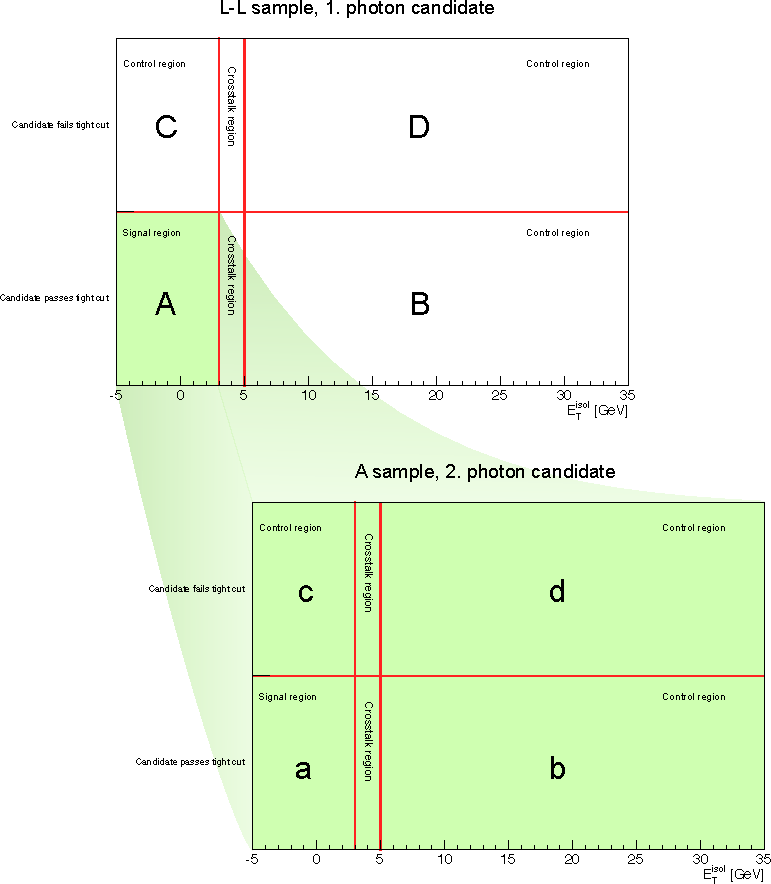
\includegraphics[width=\textwidth]{figures/sideband}
  \caption{Illustrating the two--step ABCD method, adapted from \cite{fdirect} using the `tight' selection criteria and the isolation energy: the full set of diphotons (the L-L sample) is split into four groups---A, B, C and D---according to the discriminating variables for the leading photon. Signal photons are now confined to the A region. The events in the C region can be used to estimate the shape, and the B and D region can be used to estimate the magnitude of the distribution of background events in the signal region. The procedure is then repeated for the subleading partner photons of the events in the A region. This gives an estimate of the distibution of background events in the combined signal (AA) region.}\label{abcd}
\end{figure}

This is also known as the two--dimensional sideband method \cite{cmsabcd}. The following description may be aided by the illustration in figure~\ref{abcd}.

To reiterate, we need to examine our sample of signal and background data points in terms of two uncorrelated discriminating variables, call them $x$ and $y$. With this, we can split the data set into four regions:

\begin{itemize}
\item[{\bfseries\sffamily\color{natgreen}A:}] The signal region in both discriminating variables. This region should contain all signal events.
\item[{\bfseries\sffamily\color{natgreen}B:}] The signal region in the $y$ variable, but not in $x$. We assume that the distribution of background events in $y$ in this regions will have the same shape as the distribution of background events in $y$ in the signal region, A.
\item[{\bfseries\sffamily\color{natgreen}C:}] As above, but with $x$ and $y$ exchanged.
\item[{\bfseries\sffamily\color{natgreen}D:}] The control region for both variables. Once again, we assume that the distribution of background events has the same shape for either variable in the control region as it has in its signal region. We expect the distribution in $x$ to have the same shape in the D region as it does in the B region, for example.
\end{itemize}

Thus, the distribution in $x$ of background events in the A region, $A_{bck}$, is assumed to be the shape of the distribution of events in the C region, scaled so that the distribution of events in $x$ in the B and D regions have the same magnitude:
\(A_{bck}=C\frac BD.\label{abckfind}\)
The signal distribution must then be given as
\(A_{sig}=A-A_{bck}.\label{asig}\)

As we are working with events with two photons, both of which give rise to independent backgrounds, this procedure must be repeated for the subleading photons as well. For the subleading photon candidate, we look at the sample of photon candidates that are the subleading partner of a selected photon in the signal, A, region of the distribution of leading photon candidates. Carrying out the ABCD procedure on the sample of subleading photons gives us $AA_{bck}$, an estimate of the number of selected photon pairs where the leading photon is in the A region and the subleading photon is a part of the background in the AA region.
Using \eqref{asig}, we can now write the number of events in the signal--signal region as
\(\begin{aligned}
A_{sig}A_{sig} &=(A-A_{bck})A-(A-A_{bck})A_{bck}\\ &=AA-A_{bck}A-AA_{bck}+A_{bck}A_{bck}\\&=AA-[AA]_{bck}.
\end{aligned}\)
$AA$ is the number of events in the AA region, which is readily available. Of the terms that contribute to the total background $[AA]_{bkc}$, $AA_{bck}$, the total number of background subleading photons in the AA region, is determined by taking
\(AA_{bck}=AC\frac{AB}{AD},\)
analogous to how $A_{bck}$ sample was found in eq.~\eqref{abckfind}. We find $A_{bck}A$, the total number background leading photons in the AA region, and $A_{bck}A_{bck}$, the number of photon pairs in the AA region where both members are background photons, by multiplying $AA$ and $AA_{bck}$ by
\(f_{bck}=\frac{A_{bck}}{A},\)
the fraction of background events in the leading photon A sample. Thus, the total estimated background in the AA region is given by
\([AA]_{bck}=\frac{A_{bck}}{A}(AA)+AA_{bck}-\frac{A_{bck}}{A}(AA_{bck}),\)
which we can interpret as the number of data points where the leading photon was a background plus the number of data points where the subleading photon was a background, subtracted the number of data points where both photons were background events, which would have been double counted.

For the diphoton sample, the choice of the two discriminants are the `tight' selection criteria, which were described in chapter~\ref{ch.exp}, and the transverse isolation energy, $E_T^{\text{isol}}$, the energy deposited in the calorimeter in a cone with radius $R\le0.4$, but outside $R\le0.2$, where
\[R=\sqrt{\Delta\phi^2+\Delta\theta^2}.\]
The signal region is defined as $E_T^{\text{isol}}\le3$ GeV. Allowing a crosstalk region of 2 GeV, which means the background region is $5\text{ GeV}\le E_T^{\text{isol}}\le25\text{ GeV}$, produces the distribution of $E_T^{\text{isol}}$ for leading photons and subleading photons in the `A' sample is given in figure~\ref{etiso}. As the figure shows, the tight and loose selections are identical in the background region, whereas they diverge in the crosstalk region, which is the desired behaviour.

\begin{figure}[htp]
\begin{minipage}[b]{.69\textwidth}
\begin{infilsf} \tiny 
\begin{tikzpicture}[x=.1\textwidth,y=.1\textwidth]
\pgfdeclareplotmark{cross} {
\pgfpathmoveto{\pgfpoint{-0.3\pgfplotmarksize}{\pgfplotmarksize}}
\pgfpathlineto{\pgfpoint{+0.3\pgfplotmarksize}{\pgfplotmarksize}}
\pgfpathlineto{\pgfpoint{+0.3\pgfplotmarksize}{0.3\pgfplotmarksize}}
\pgfpathlineto{\pgfpoint{+1\pgfplotmarksize}{0.3\pgfplotmarksize}}
\pgfpathlineto{\pgfpoint{+1\pgfplotmarksize}{-0.3\pgfplotmarksize}}
\pgfpathlineto{\pgfpoint{+0.3\pgfplotmarksize}{-0.3\pgfplotmarksize}}
\pgfpathlineto{\pgfpoint{+0.3\pgfplotmarksize}{-1.\pgfplotmarksize}}
\pgfpathlineto{\pgfpoint{-0.3\pgfplotmarksize}{-1.\pgfplotmarksize}}
\pgfpathlineto{\pgfpoint{-0.3\pgfplotmarksize}{-0.3\pgfplotmarksize}}
\pgfpathlineto{\pgfpoint{-1.\pgfplotmarksize}{-0.3\pgfplotmarksize}}
\pgfpathlineto{\pgfpoint{-1.\pgfplotmarksize}{0.3\pgfplotmarksize}}
\pgfpathlineto{\pgfpoint{-0.3\pgfplotmarksize}{0.3\pgfplotmarksize}}
\pgfpathclose
\pgfusepathqstroke
}
\pgfdeclareplotmark{cross*} {
\pgfpathmoveto{\pgfpoint{-0.3\pgfplotmarksize}{\pgfplotmarksize}}
\pgfpathlineto{\pgfpoint{+0.3\pgfplotmarksize}{\pgfplotmarksize}}
\pgfpathlineto{\pgfpoint{+0.3\pgfplotmarksize}{0.3\pgfplotmarksize}}
\pgfpathlineto{\pgfpoint{+1\pgfplotmarksize}{0.3\pgfplotmarksize}}
\pgfpathlineto{\pgfpoint{+1\pgfplotmarksize}{-0.3\pgfplotmarksize}}
\pgfpathlineto{\pgfpoint{+0.3\pgfplotmarksize}{-0.3\pgfplotmarksize}}
\pgfpathlineto{\pgfpoint{+0.3\pgfplotmarksize}{-1.\pgfplotmarksize}}
\pgfpathlineto{\pgfpoint{-0.3\pgfplotmarksize}{-1.\pgfplotmarksize}}
\pgfpathlineto{\pgfpoint{-0.3\pgfplotmarksize}{-0.3\pgfplotmarksize}}
\pgfpathlineto{\pgfpoint{-1.\pgfplotmarksize}{-0.3\pgfplotmarksize}}
\pgfpathlineto{\pgfpoint{-1.\pgfplotmarksize}{0.3\pgfplotmarksize}}
\pgfpathlineto{\pgfpoint{-0.3\pgfplotmarksize}{0.3\pgfplotmarksize}}
\pgfpathclose
\pgfusepathqfillstroke
}
\pgfdeclareplotmark{newstar} {
\pgfpathmoveto{\pgfqpoint{0pt}{\pgfplotmarksize}}
\pgfpathlineto{\pgfqpointpolar{44}{0.5\pgfplotmarksize}}
\pgfpathlineto{\pgfqpointpolar{18}{\pgfplotmarksize}}
\pgfpathlineto{\pgfqpointpolar{-20}{0.5\pgfplotmarksize}}
\pgfpathlineto{\pgfqpointpolar{-54}{\pgfplotmarksize}}
\pgfpathlineto{\pgfqpointpolar{-90}{0.5\pgfplotmarksize}}
\pgfpathlineto{\pgfqpointpolar{234}{\pgfplotmarksize}}
\pgfpathlineto{\pgfqpointpolar{198}{0.5\pgfplotmarksize}}
\pgfpathlineto{\pgfqpointpolar{162}{\pgfplotmarksize}}
\pgfpathlineto{\pgfqpointpolar{134}{0.5\pgfplotmarksize}}
\pgfpathclose
\pgfusepathqstroke
}
\pgfdeclareplotmark{newstar*} {
\pgfpathmoveto{\pgfqpoint{0pt}{\pgfplotmarksize}}
\pgfpathlineto{\pgfqpointpolar{44}{0.5\pgfplotmarksize}}
\pgfpathlineto{\pgfqpointpolar{18}{\pgfplotmarksize}}
\pgfpathlineto{\pgfqpointpolar{-20}{0.5\pgfplotmarksize}}
\pgfpathlineto{\pgfqpointpolar{-54}{\pgfplotmarksize}}
\pgfpathlineto{\pgfqpointpolar{-90}{0.5\pgfplotmarksize}}
\pgfpathlineto{\pgfqpointpolar{234}{\pgfplotmarksize}}
\pgfpathlineto{\pgfqpointpolar{198}{0.5\pgfplotmarksize}}
\pgfpathlineto{\pgfqpointpolar{162}{\pgfplotmarksize}}
\pgfpathlineto{\pgfqpointpolar{134}{0.5\pgfplotmarksize}}
\pgfpathclose
\pgfusepathqfillstroke
}
\definecolor{c}{rgb}{1,1,1};
\draw [color=c, fill=c] (1,0.679598) rectangle (9,6.11638);
\definecolor{c}{rgb}{0,0,0};
\draw [c] (1,0.679598) -- (1,6.11638) -- (9,6.11638) -- (9,0.679598) -- (1,0.679598);
\definecolor{c}{rgb}{1,1,1};
\draw [color=c, fill=c] (1,0.679598) rectangle (9,6.11638);
\definecolor{c}{rgb}{0,0,0};
\draw [c] (1,0.679598) -- (1,6.11638) -- (9,6.11638) -- (9,0.679598) -- (1,0.679598);
\colorlet{c}{natgreen}
\draw [c] (1,0.680318) -- (1.0293,0.680318) -- (1.0293,0.681757) -- (1.05861,0.681757) -- (1.05861,0.681757) -- (1.08791,0.681757) -- (1.08791,0.683197) -- (1.11722,0.683197) -- (1.11722,0.682837) -- (1.14652,0.682837) -- (1.14652,0.682837) --
 (1.17582,0.682837) -- (1.17582,0.684637) -- (1.20513,0.684637) -- (1.20513,0.686437) -- (1.23443,0.686437) -- (1.23443,0.689676) -- (1.26374,0.689676) -- (1.26374,0.691476) -- (1.29304,0.691476) -- (1.29304,0.692916) -- (1.32234,0.692916) --
 (1.32234,0.700115) -- (1.35165,0.700115) -- (1.35165,0.706594) -- (1.38095,0.706594) -- (1.38095,0.718832) -- (1.41026,0.718832) -- (1.41026,0.730711) -- (1.43956,0.730711) -- (1.43956,0.73251) -- (1.46886,0.73251) -- (1.46886,0.749428) --
 (1.49817,0.749428) -- (1.49817,0.765986) -- (1.52747,0.765986) -- (1.52747,0.803421) -- (1.55678,0.803421) -- (1.55678,0.825378) -- (1.58608,0.825378) -- (1.58608,0.872891) -- (1.61538,0.872891) -- (1.61538,0.916085) -- (1.64469,0.916085) --
 (1.64469,0.980156) -- (1.67399,0.980156) -- (1.67399,1.02983) -- (1.7033,1.02983) -- (1.7033,1.13098) -- (1.7326,1.13098) -- (1.7326,1.24976) -- (1.7619,1.24976) -- (1.7619,1.36998) -- (1.79121,1.36998) -- (1.79121,1.47797) -- (1.82051,1.47797) --
 (1.82051,1.70258) -- (1.84982,1.70258) -- (1.84982,1.88471) -- (1.87912,1.88471) -- (1.87912,2.13668) -- (1.90842,2.13668) -- (1.90842,2.44264) -- (1.93773,2.44264) -- (1.93773,2.74931) -- (1.96703,2.74931) -- (1.96703,3.11538) -- (1.99634,3.11538)
 -- (1.99634,3.51025) -- (2.02564,3.51025) -- (2.02564,3.91339) -- (2.05494,3.91339) -- (2.05494,4.39969) -- (2.08425,4.39969) -- (2.08425,4.83019) -- (2.11355,4.83019) -- (2.11355,5.25133) -- (2.14286,5.25133) -- (2.14286,5.5742) -- (2.17216,5.5742)
 -- (2.17216,5.74302) -- (2.20147,5.74302) -- (2.20147,5.85748) -- (2.23077,5.85748) -- (2.23077,5.71314) -- (2.26007,5.71314) -- (2.26007,5.43346) -- (2.28938,5.43346) -- (2.28938,5.30064) -- (2.31868,5.30064) -- (2.31868,5.13362) --
 (2.34799,5.13362) -- (2.34799,4.86654) -- (2.37729,4.86654) -- (2.37729,4.65165) -- (2.40659,4.65165) -- (2.40659,4.41552) -- (2.4359,4.41552) -- (2.4359,4.16608) -- (2.4652,4.16608) -- (2.4652,4.03974) -- (2.49451,4.03974) -- (2.49451,3.90655) --
 (2.52381,3.90655) -- (2.52381,3.68158) -- (2.55311,3.68158) -- (2.55311,3.57216) -- (2.58242,3.57216) -- (2.58242,3.35511) -- (2.61172,3.35511) -- (2.61172,3.31767) -- (2.64103,3.31767) -- (2.64103,3.12546) -- (2.67033,3.12546) -- (2.67033,2.98292)
 -- (2.69963,2.98292) -- (2.69963,2.8429) -- (2.72894,2.8429) -- (2.72894,2.79683) -- (2.75824,2.79683) -- (2.75824,2.59309) -- (2.78755,2.59309) -- (2.78755,2.60389) -- (2.81685,2.60389) -- (2.81685,2.42572) -- (2.84615,2.42572) -- (2.84615,2.37208)
 -- (2.87546,2.37208) -- (2.87546,2.2821) -- (2.90476,2.2821) -- (2.90476,2.19823) -- (2.93407,2.19823) -- (2.93407,2.105) -- (2.96337,2.105) -- (2.96337,2.07477) -- (2.99267,2.07477) -- (2.99267,1.9513) -- (3.02198,1.9513) -- (3.02198,1.91567) --
 (3.05128,1.91567) -- (3.05128,1.8552) -- (3.08059,1.8552) -- (3.08059,1.80192) -- (3.10989,1.80192) -- (3.10989,1.72813) -- (3.13919,1.72813) -- (3.13919,1.70582) -- (3.1685,1.70582) -- (3.1685,1.66298) -- (3.1978,1.66298) -- (3.1978,1.60575) --
 (3.22711,1.60575) -- (3.22711,1.58127) -- (3.25641,1.58127) -- (3.25641,1.53772) -- (3.28571,1.53772) -- (3.28571,1.48373) -- (3.31502,1.48373) -- (3.31502,1.43441) -- (3.34432,1.43441) -- (3.34432,1.44557) -- (3.37363,1.44557) -- (3.37363,1.37754)
 -- (3.40293,1.37754) -- (3.40293,1.35594) -- (3.43223,1.35594) -- (3.43223,1.32931) -- (3.46154,1.32931) -- (3.46154,1.29151) -- (3.49084,1.29151) -- (3.49084,1.30159) -- (3.52015,1.30159) -- (3.52015,1.23608) -- (3.54945,1.23608) --
 (3.54945,1.2476) -- (3.57875,1.2476) -- (3.57875,1.20405) -- (3.60806,1.20405) -- (3.60806,1.19361) -- (3.63736,1.19361) -- (3.63736,1.19181) -- (3.66667,1.19181) -- (3.66667,1.18497) -- (3.69597,1.18497) -- (3.69597,1.14357) -- (3.72527,1.14357) --
 (3.72527,1.11766) -- (3.75458,1.11766) -- (3.75458,1.10074) -- (3.78388,1.10074) -- (3.78388,1.0705) -- (3.81319,1.0705) -- (3.81319,1.08454) -- (3.84249,1.08454) -- (3.84249,1.04675) -- (3.87179,1.04675) -- (3.87179,1.03523) -- (3.9011,1.03523) --
 (3.9011,1.01651) -- (3.9304,1.01651) -- (3.9304,1.01939) -- (3.95971,1.01939) -- (3.95971,1.01039) -- (3.98901,1.01039) -- (3.98901,1.01363) -- (4.01831,1.01363) -- (4.01831,0.979796) -- (4.04762,0.979796) -- (4.04762,0.969358) -- (4.07692,0.969358)
 -- (4.07692,0.944881) -- (4.10623,0.944881) -- (4.10623,0.95316) -- (4.13553,0.95316) -- (4.13553,0.927604) -- (4.16483,0.927604) -- (4.16483,0.927244) -- (4.19414,0.927244) -- (4.19414,0.899168) -- (4.22344,0.899168) -- (4.22344,0.907446) --
 (4.25275,0.907446) -- (4.25275,0.914285) -- (4.28205,0.914285) -- (4.28205,0.890529) -- (4.31136,0.890529) -- (4.31136,0.901687) -- (4.34066,0.901687) -- (4.34066,0.898088) -- (4.36996,0.898088) -- (4.36996,0.88369) -- (4.39927,0.88369) --
 (4.39927,0.87793) -- (4.42857,0.87793) -- (4.42857,0.867852) -- (4.45788,0.867852) -- (4.45788,0.859573) -- (4.48718,0.859573) -- (4.48718,0.850574) -- (4.51648,0.850574) -- (4.51648,0.849854) -- (4.54579,0.849854) -- (4.54579,0.854174) --
 (4.57509,0.854174) -- (4.57509,0.852014) -- (4.6044,0.852014) -- (4.6044,0.847695) -- (4.6337,0.847695) -- (4.6337,0.823578) -- (4.663,0.823578) -- (4.663,0.833297) -- (4.69231,0.833297) -- (4.69231,0.818539) -- (4.72161,0.818539) --
 (4.72161,0.802701) -- (4.75092,0.802701) -- (4.75092,0.818539) -- (4.78022,0.818539) -- (4.78022,0.813499) -- (4.80952,0.813499) -- (4.80952,0.81134) -- (4.83883,0.81134) -- (4.83883,0.799101) -- (4.86813,0.799101) -- (4.86813,0.789743) --
 (4.89744,0.789743) -- (4.89744,0.796942) -- (4.92674,0.796942) -- (4.92674,0.792262) -- (4.95604,0.792262) -- (4.95604,0.795502) -- (4.98535,0.795502) -- (4.98535,0.797661) -- (5.01465,0.797661) -- (5.01465,0.777144) -- (5.04396,0.777144) --
 (5.04396,0.783983) -- (5.07326,0.783983) -- (5.07326,0.776784) -- (5.10256,0.776784) -- (5.10256,0.770305) -- (5.13187,0.770305) -- (5.13187,0.773545) -- (5.16117,0.773545) -- (5.16117,0.778584) -- (5.19048,0.778584) -- (5.19048,0.772465) --
 (5.21978,0.772465) -- (5.21978,0.764186) -- (5.24908,0.764186) -- (5.24908,0.763106) -- (5.27839,0.763106) -- (5.27839,0.760227) -- (5.30769,0.760227) -- (5.30769,0.762026) -- (5.337,0.762026) -- (5.337,0.756627) -- (5.3663,0.756627) --
 (5.3663,0.762746) -- (5.3956,0.762746) -- (5.3956,0.757707) -- (5.42491,0.757707) -- (5.42491,0.755187) -- (5.45421,0.755187) -- (5.45421,0.747628) -- (5.48352,0.747628) -- (5.48352,0.745469) -- (5.51282,0.745469) -- (5.51282,0.747268) --
 (5.54212,0.747268) -- (5.54212,0.753388) -- (5.57143,0.753388) -- (5.57143,0.746908) -- (5.60073,0.746908) -- (5.60073,0.73827) -- (5.63004,0.73827) -- (5.63004,0.741869) -- (5.65934,0.741869) -- (5.65934,0.742229) -- (5.68864,0.742229) --
 (5.68864,0.739709) -- (5.71795,0.739709) -- (5.71795,0.73863) -- (5.74725,0.73863) -- (5.74725,0.731431) -- (5.77656,0.731431) -- (5.77656,0.728551) -- (5.80586,0.728551) -- (5.80586,0.731431) -- (5.83517,0.731431) -- (5.83517,0.731791) --
 (5.86447,0.731791) -- (5.86447,0.730351) -- (5.89377,0.730351) -- (5.89377,0.725671) -- (5.92308,0.725671) -- (5.92308,0.73935) -- (5.95238,0.73935) -- (5.95238,0.731791) -- (5.98169,0.731791) -- (5.98169,0.727111) -- (6.01099,0.727111) --
 (6.01099,0.728551) -- (6.04029,0.728551) -- (6.04029,0.73467) -- (6.0696,0.73467) -- (6.0696,0.723152) -- (6.0989,0.723152) -- (6.0989,0.728191) -- (6.12821,0.728191) -- (6.12821,0.722792) -- (6.15751,0.722792) -- (6.15751,0.726391) --
 (6.18681,0.726391) -- (6.18681,0.720632) -- (6.21612,0.720632) -- (6.21612,0.717033) -- (6.24542,0.717033) -- (6.24542,0.722432) -- (6.27473,0.722432) -- (6.27473,0.715593) -- (6.30403,0.715593) -- (6.30403,0.719552) -- (6.33333,0.719552) --
 (6.33333,0.717753) -- (6.36264,0.717753) -- (6.36264,0.717393) -- (6.39194,0.717393) -- (6.39194,0.714153) -- (6.42125,0.714153) -- (6.42125,0.716673) -- (6.45055,0.716673) -- (6.45055,0.713433) -- (6.47985,0.713433) -- (6.47985,0.719192) --
 (6.50916,0.719192) -- (6.50916,0.712353) -- (6.53846,0.712353) -- (6.53846,0.713793) -- (6.56777,0.713793) -- (6.56777,0.715593) -- (6.59707,0.715593) -- (6.59707,0.710194) -- (6.62637,0.710194) -- (6.62637,0.718832) -- (6.65568,0.718832) --
 (6.65568,0.713793) -- (6.68498,0.713793) -- (6.68498,0.706954) -- (6.71429,0.706954) -- (6.71429,0.715593) -- (6.74359,0.715593) -- (6.74359,0.708394) -- (6.77289,0.708394) -- (6.77289,0.711633) -- (6.8022,0.711633) -- (6.8022,0.708394) --
 (6.8315,0.708394) -- (6.8315,0.705154) -- (6.86081,0.705154) -- (6.86081,0.707314) -- (6.89011,0.707314) -- (6.89011,0.711633) -- (6.91941,0.711633) -- (6.91941,0.709834) -- (6.94872,0.709834) -- (6.94872,0.707314) -- (6.97802,0.707314) --
 (6.97802,0.707314) -- (7.00733,0.707314) -- (7.00733,0.704434) -- (7.03663,0.704434) -- (7.03663,0.707314) -- (7.06593,0.707314) -- (7.06593,0.706954) -- (7.09524,0.706954) -- (7.09524,0.703354) -- (7.12454,0.703354) -- (7.12454,0.704794) --
 (7.15385,0.704794) -- (7.15385,0.708754) -- (7.18315,0.708754) -- (7.18315,0.703714) -- (7.21245,0.703714) -- (7.21245,0.709834) -- (7.24176,0.709834) -- (7.24176,0.699755) -- (7.27106,0.699755) -- (7.27106,0.702275) -- (7.30037,0.702275) --
 (7.30037,0.704074) -- (7.32967,0.704074) -- (7.32967,0.700835) -- (7.35897,0.700835) -- (7.35897,0.703354) -- (7.38828,0.703354) -- (7.38828,0.705514) -- (7.41758,0.705514) -- (7.41758,0.696155) -- (7.44689,0.696155) -- (7.44689,0.697595) --
 (7.47619,0.697595) -- (7.47619,0.708034) -- (7.50549,0.708034) -- (7.50549,0.700835) -- (7.5348,0.700835) -- (7.5348,0.700115) -- (7.5641,0.700115) -- (7.5641,0.698315) -- (7.59341,0.698315) -- (7.59341,0.697955) -- (7.62271,0.697955) --
 (7.62271,0.700835) -- (7.65201,0.700835) -- (7.65201,0.702635) -- (7.68132,0.702635) -- (7.68132,0.694716) -- (7.71062,0.694716) -- (7.71062,0.698315) -- (7.73993,0.698315) -- (7.73993,0.703354) -- (7.76923,0.703354) -- (7.76923,0.694716) --
 (7.79853,0.694716) -- (7.79853,0.699035) -- (7.82784,0.699035) -- (7.82784,0.697955) -- (7.85714,0.697955) -- (7.85714,0.697955) -- (7.88645,0.697955) -- (7.88645,0.699755) -- (7.91575,0.699755) -- (7.91575,0.701195) -- (7.94506,0.701195) --
 (7.94506,0.699755) -- (7.97436,0.699755) -- (7.97436,0.694356) -- (8.00366,0.694356) -- (8.00366,0.697955) -- (8.03297,0.697955) -- (8.03297,0.696515) -- (8.06227,0.696515) -- (8.06227,0.697595) -- (8.09157,0.697595) -- (8.09157,0.694356) --
 (8.12088,0.694356) -- (8.12088,0.699395) -- (8.15018,0.699395) -- (8.15018,0.695076) -- (8.17949,0.695076) -- (8.17949,0.695796) -- (8.20879,0.695796) -- (8.20879,0.695436) -- (8.2381,0.695436) -- (8.2381,0.697235) -- (8.2674,0.697235) --
 (8.2674,0.694716) -- (8.2967,0.694716) -- (8.2967,0.694356) -- (8.32601,0.694356) -- (8.32601,0.692556) -- (8.35531,0.692556) -- (8.35531,0.692196) -- (8.38461,0.692196) -- (8.38461,0.695076) -- (8.41392,0.695076) -- (8.41392,0.697235) --
 (8.44322,0.697235) -- (8.44322,0.694716) -- (8.47253,0.694716) -- (8.47253,0.696155) -- (8.50183,0.696155) -- (8.50183,0.694716) -- (8.53114,0.694716) -- (8.53114,0.696155) -- (8.56044,0.696155) -- (8.56044,0.692916) -- (8.58974,0.692916) --
 (8.58974,0.693276) -- (8.61905,0.693276) -- (8.61905,0.688596) -- (8.64835,0.688596) -- (8.64835,0.691476) -- (8.67766,0.691476) -- (8.67766,0.690756) -- (8.70696,0.690756) -- (8.70696,0.688956) -- (8.73626,0.688956) -- (8.73626,0.691476) --
 (8.76557,0.691476) -- (8.76557,0.691476) -- (8.79487,0.691476) -- (8.79487,0.695796) -- (8.82418,0.695796) -- (8.82418,0.692556) -- (8.85348,0.692556) -- (8.85348,0.692556) -- (8.88278,0.692556) -- (8.88278,0.693996) -- (8.91209,0.693996) --
 (8.91209,0.695076) -- (8.94139,0.695076) -- (8.94139,0.689676) -- (8.9707,0.689676) -- (8.9707,0.691116) -- (9,0.691116);
\definecolor{c}{rgb}{0,0,0};
\draw [c] (1,0.679598) -- (9,0.679598);
\draw [anchor= east] (9,0.299023) node[color=c, rotate=0]{$E_{T}^{\text{isol}}$ [GeV]};
\draw [c] (1,0.842701) -- (1,0.679598);
\draw [c] (1.2664,0.761149) -- (1.2664,0.679598);
\draw [c] (1.5328,0.761149) -- (1.5328,0.679598);
\draw [c] (1.7992,0.761149) -- (1.7992,0.679598);
\draw [c] (2.0656,0.761149) -- (2.0656,0.679598);
\draw [c] (2.332,0.842701) -- (2.332,0.679598);
\draw [c] (2.5984,0.761149) -- (2.5984,0.679598);
\draw [c] (2.8648,0.761149) -- (2.8648,0.679598);
\draw [c] (3.1312,0.761149) -- (3.1312,0.679598);
\draw [c] (3.3976,0.761149) -- (3.3976,0.679598);
\draw [c] (3.664,0.842701) -- (3.664,0.679598);
\draw [c] (3.9304,0.761149) -- (3.9304,0.679598);
\draw [c] (4.1968,0.761149) -- (4.1968,0.679598);
\draw [c] (4.4632,0.761149) -- (4.4632,0.679598);
\draw [c] (4.7296,0.761149) -- (4.7296,0.679598);
\draw [c] (4.996,0.842701) -- (4.996,0.679598);
\draw [c] (5.2624,0.761149) -- (5.2624,0.679598);
\draw [c] (5.5288,0.761149) -- (5.5288,0.679598);
\draw [c] (5.7952,0.761149) -- (5.7952,0.679598);
\draw [c] (6.0616,0.761149) -- (6.0616,0.679598);
\draw [c] (6.32801,0.842701) -- (6.32801,0.679598);
\draw [c] (6.59441,0.761149) -- (6.59441,0.679598);
\draw [c] (6.86081,0.761149) -- (6.86081,0.679598);
\draw [c] (7.12721,0.761149) -- (7.12721,0.679598);
\draw [c] (7.39361,0.761149) -- (7.39361,0.679598);
\draw [c] (7.66001,0.842701) -- (7.66001,0.679598);
\draw [c] (7.92641,0.761149) -- (7.92641,0.679598);
\draw [c] (8.19281,0.761149) -- (8.19281,0.679598);
\draw [c] (8.45921,0.761149) -- (8.45921,0.679598);
\draw [c] (8.72561,0.761149) -- (8.72561,0.679598);
\draw [c] (8.99201,0.842701) -- (8.99201,0.679598);
\draw [c] (8.99201,0.842701) -- (8.99201,0.679598);
\draw [anchor=base] (1,0.455331) node[color=c, rotate=0]{-5};
\draw [anchor=base] (2.332,0.455331) node[color=c, rotate=0]{0};
\draw [anchor=base] (3.664,0.455331) node[color=c, rotate=0]{5};
\draw [anchor=base] (4.996,0.455331) node[color=c, rotate=0]{10};
\draw [anchor=base] (6.32801,0.455331) node[color=c, rotate=0]{15};
\draw [anchor=base] (7.66001,0.455331) node[color=c, rotate=0]{20};
\draw [anchor=base] (8.99201,0.455331) node[color=c, rotate=0]{25};
\draw [c] (1,0.679598) -- (1,6.11638);
\draw [anchor= east] (0.0,6.11638) node[color=c, rotate=90]{Number of events};
\draw [c] (1.24,0.679598) -- (1,0.679598);
\draw [c] (1.12,0.859573) -- (1,0.859573);
\draw [c] (1.12,1.03955) -- (1,1.03955);
\draw [c] (1.12,1.21952) -- (1,1.21952);
\draw [c] (1.24,1.3995) -- (1,1.3995);
\draw [c] (1.12,1.57947) -- (1,1.57947);
\draw [c] (1.12,1.75945) -- (1,1.75945);
\draw [c] (1.12,1.93942) -- (1,1.93942);
\draw [c] (1.24,2.1194) -- (1,2.1194);
\draw [c] (1.12,2.29937) -- (1,2.29937);
\draw [c] (1.12,2.47935) -- (1,2.47935);
\draw [c] (1.12,2.65933) -- (1,2.65933);
\draw [c] (1.24,2.8393) -- (1,2.8393);
\draw [c] (1.12,3.01928) -- (1,3.01928);
\draw [c] (1.12,3.19925) -- (1,3.19925);
\draw [c] (1.12,3.37923) -- (1,3.37923);
\draw [c] (1.24,3.5592) -- (1,3.5592);
\draw [c] (1.12,3.73918) -- (1,3.73918);
\draw [c] (1.12,3.91915) -- (1,3.91915);
\draw [c] (1.12,4.09913) -- (1,4.09913);
\draw [c] (1.24,4.2791) -- (1,4.2791);
\draw [c] (1.12,4.45908) -- (1,4.45908);
\draw [c] (1.12,4.63905) -- (1,4.63905);
\draw [c] (1.12,4.81903) -- (1,4.81903);
\draw [c] (1.24,4.999) -- (1,4.999);
\draw [c] (1.12,5.17898) -- (1,5.17898);
\draw [c] (1.12,5.35895) -- (1,5.35895);
\draw [c] (1.12,5.53893) -- (1,5.53893);
\draw [c] (1.24,5.7189) -- (1,5.7189);
\draw [c] (1.24,5.7189) -- (1,5.7189);
\draw [c] (1.12,5.89888) -- (1,5.89888);
\draw [c] (1.12,6.07885) -- (1,6.07885);
\draw [anchor= east] (0.95,0.679598) node[color=c, rotate=0]{0};
\draw [anchor= east] (0.95,1.3995) node[color=c, rotate=0]{2000};
\draw [anchor= east] (0.95,2.1194) node[color=c, rotate=0]{4000};
\draw [anchor= east] (0.95,2.8393) node[color=c, rotate=0]{6000};
\draw [anchor= east] (0.95,3.5592) node[color=c, rotate=0]{8000};
\draw [anchor= east] (0.95,4.2791) node[color=c, rotate=0]{10000};
\draw [anchor= east] (0.95,4.999) node[color=c, rotate=0]{12000};
\draw [anchor= east] (0.95,5.7189) node[color=c, rotate=0]{14000};
\colorlet{c}{natgreen!50}
\draw [c] (1,0.679598) -- (1.0293,0.679598) -- (1.0293,0.679598) -- (1.05861,0.679598) -- (1.05861,0.679598) -- (1.08791,0.679598) -- (1.08791,0.679598) -- (1.11722,0.679598) -- (1.11722,0.679598) -- (1.14652,0.679598) -- (1.14652,0.679598) --
 (1.17582,0.679598) -- (1.17582,0.679598) -- (1.20513,0.679598) -- (1.20513,0.680546) -- (1.23443,0.680546) -- (1.23443,0.680546) -- (1.26374,0.680546) -- (1.26374,0.681359) -- (1.29304,0.681359) -- (1.29304,0.682307) -- (1.32234,0.682307) --
 (1.32234,0.683526) -- (1.35165,0.683526) -- (1.35165,0.684745) -- (1.38095,0.684745) -- (1.38095,0.683932) -- (1.41026,0.683932) -- (1.41026,0.684339) -- (1.43956,0.684339) -- (1.43956,0.688267) -- (1.46886,0.688267) -- (1.46886,0.688809) --
 (1.49817,0.688809) -- (1.49817,0.694227) -- (1.52747,0.694227) -- (1.52747,0.694633) -- (1.55678,0.694633) -- (1.55678,0.700457) -- (1.58608,0.700457) -- (1.58608,0.707366) -- (1.61538,0.707366) -- (1.61538,0.715899) -- (1.64469,0.715899) --
 (1.64469,0.72362) -- (1.67399,0.72362) -- (1.67399,0.733643) -- (1.7033,0.733643) -- (1.7033,0.745834) -- (1.7326,0.745834) -- (1.7326,0.760327) -- (1.7619,0.760327) -- (1.7619,0.777665) -- (1.79121,0.777665) -- (1.79121,0.800963) --
 (1.82051,0.800963) -- (1.82051,0.835368) -- (1.84982,0.835368) -- (1.84982,0.859885) -- (1.87912,0.859885) -- (1.87912,0.894425) -- (1.90842,0.894425) -- (1.90842,0.9333) -- (1.93773,0.9333) -- (1.93773,0.997098) -- (1.96703,0.997098) --
 (1.96703,1.04207) -- (1.99634,1.04207) -- (1.99634,1.10776) -- (2.02564,1.10776) -- (2.02564,1.17413) -- (2.05494,1.17413) -- (2.05494,1.23211) -- (2.08425,1.23211) -- (2.08425,1.31907) -- (2.11355,1.31907) -- (2.11355,1.41091) -- (2.14286,1.41091)
 -- (2.14286,1.46563) -- (2.17216,1.46563) -- (2.17216,1.54798) -- (2.20147,1.54798) -- (2.20147,1.60487) -- (2.23077,1.60487) -- (2.23077,1.64267) -- (2.26007,1.64267) -- (2.26007,1.69346) -- (2.28938,1.69346) -- (2.28938,1.7471) -- (2.31868,1.7471)
 -- (2.31868,1.76268) -- (2.34799,1.76268) -- (2.34799,1.76769) -- (2.37729,1.76769) -- (2.37729,1.81401) -- (2.40659,1.81401) -- (2.40659,1.84151) -- (2.4359,1.84151) -- (2.4359,1.82675) -- (2.4652,1.82675) -- (2.4652,1.85478) -- (2.49451,1.85478)
 -- (2.49451,1.8407) -- (2.52381,1.8407) -- (2.52381,1.83988) -- (2.55311,1.83988) -- (2.55311,1.82796) -- (2.58242,1.82796) -- (2.58242,1.85668) -- (2.61172,1.85668) -- (2.61172,1.84584) -- (2.64103,1.84584) -- (2.64103,1.82295) -- (2.67033,1.82295)
 -- (2.67033,1.79099) -- (2.69963,1.79099) -- (2.69963,1.79884) -- (2.72894,1.79884) -- (2.72894,1.78286) -- (2.75824,1.78286) -- (2.75824,1.75401) -- (2.78755,1.75401) -- (2.78755,1.75645) -- (2.81685,1.75645) -- (2.81685,1.73829) --
 (2.84615,1.73829) -- (2.84615,1.70877) -- (2.87546,1.70877) -- (2.87546,1.67368) -- (2.90476,1.67368) -- (2.90476,1.6745) -- (2.93407,1.6745) -- (2.93407,1.65161) -- (2.96337,1.65161) -- (2.96337,1.62763) -- (2.99267,1.62763) -- (2.99267,1.60691) --
 (3.02198,1.60691) -- (3.02198,1.59566) -- (3.05128,1.59566) -- (3.05128,1.55841) -- (3.08059,1.55841) -- (3.08059,1.53782) -- (3.10989,1.53782) -- (3.10989,1.51981) -- (3.13919,1.51981) -- (3.13919,1.47863) -- (3.1685,1.47863) -- (3.1685,1.47863) --
 (3.1978,1.47863) -- (3.1978,1.45764) -- (3.22711,1.45764) -- (3.22711,1.43163) -- (3.25641,1.43163) -- (3.25641,1.40197) -- (3.28571,1.40197) -- (3.28571,1.38693) -- (3.31502,1.38693) -- (3.31502,1.36648) -- (3.34432,1.36648) -- (3.34432,1.33844) --
 (3.37363,1.33844) -- (3.37363,1.32665) -- (3.40293,1.32665) -- (3.40293,1.30078) -- (3.43223,1.30078) -- (3.43223,1.28575) -- (3.46154,1.28575) -- (3.46154,1.27545) -- (3.49084,1.27545) -- (3.49084,1.22601) -- (3.52015,1.22601) -- (3.52015,1.22452)
 -- (3.54945,1.22452) -- (3.54945,1.21003) -- (3.57875,1.21003) -- (3.57875,1.19256) -- (3.60806,1.19256) -- (3.60806,1.18158) -- (3.63736,1.18158) -- (3.63736,1.14285) -- (3.66667,1.14285) -- (3.66667,1.14027) -- (3.69597,1.14027) --
 (3.69597,1.13011) -- (3.72527,1.13011) -- (3.72527,1.11819) -- (3.75458,1.11819) -- (3.75458,1.08243) -- (3.78388,1.08243) -- (3.78388,1.08487) -- (3.81319,1.08487) -- (3.81319,1.07525) -- (3.84249,1.07525) -- (3.84249,1.06225) -- (3.87179,1.06225)
 -- (3.87179,1.05914) -- (3.9011,1.05914) -- (3.9011,1.0315) -- (3.9304,1.0315) -- (3.9304,1.0376) -- (3.95971,1.0376) -- (3.95971,1.01985) -- (3.98901,1.01985) -- (3.98901,1.01037) -- (4.01831,1.01037) -- (4.01831,0.988565) -- (4.04762,0.988565) --
 (4.04762,0.991139) -- (4.07692,0.991139) -- (4.07692,0.977458) -- (4.10623,0.977458) -- (4.10623,0.954295) -- (4.13553,0.954295) -- (4.13553,0.941292) -- (4.16483,0.941292) -- (4.16483,0.93926) -- (4.19414,0.93926) -- (4.19414,0.940886) --
 (4.22344,0.940886) -- (4.22344,0.919078) -- (4.25275,0.919078) -- (4.25275,0.91068) -- (4.28205,0.91068) -- (4.28205,0.893613) -- (4.31136,0.893613) -- (4.31136,0.911763) -- (4.34066,0.911763) -- (4.34066,0.899031) -- (4.36996,0.899031) --
 (4.36996,0.890633) -- (4.39927,0.890633) -- (4.39927,0.878713) -- (4.42857,0.878713) -- (4.42857,0.881016) -- (4.45788,0.881016) -- (4.45788,0.874243) -- (4.48718,0.874243) -- (4.48718,0.863949) -- (4.51648,0.863949) -- (4.51648,0.865845) --
 (4.54579,0.865845) -- (4.54579,0.850403) -- (4.57509,0.850403) -- (4.57509,0.845933) -- (4.6044,0.845933) -- (4.6044,0.84187) -- (4.6337,0.84187) -- (4.6337,0.842683) -- (4.663,0.842683) -- (4.663,0.837671) -- (4.69231,0.837671) --
 (4.69231,0.831711) -- (4.72161,0.831711) -- (4.72161,0.827512) -- (4.75092,0.827512) -- (4.75092,0.813831) -- (4.78022,0.813831) -- (4.78022,0.819249) -- (4.80952,0.819249) -- (4.80952,0.805162) -- (4.83883,0.805162) -- (4.83883,0.810987) --
 (4.86813,0.810987) -- (4.86813,0.809497) -- (4.89744,0.809497) -- (4.89744,0.80462) -- (4.92674,0.80462) -- (4.92674,0.801776) -- (4.95604,0.801776) -- (4.95604,0.794191) -- (4.98535,0.794191) -- (4.98535,0.80313) -- (5.01465,0.80313) --
 (5.01465,0.788231) -- (5.04396,0.788231) -- (5.04396,0.78051) -- (5.07326,0.78051) -- (5.07326,0.781458) -- (5.10256,0.781458) -- (5.10256,0.78349) -- (5.13187,0.78349) -- (5.13187,0.786741) -- (5.16117,0.786741) -- (5.16117,0.775634) --
 (5.19048,0.775634) -- (5.19048,0.775363) -- (5.21978,0.775363) -- (5.21978,0.770757) -- (5.24908,0.770757) -- (5.24908,0.76561) -- (5.27839,0.76561) -- (5.27839,0.761817) -- (5.30769,0.761817) -- (5.30769,0.766694) -- (5.337,0.766694) --
 (5.337,0.759108) -- (5.3663,0.759108) -- (5.3663,0.762359) -- (5.3956,0.762359) -- (5.3956,0.756535) -- (5.42491,0.756535) -- (5.42491,0.757889) -- (5.45421,0.757889) -- (5.45421,0.751929) -- (5.48352,0.751929) -- (5.48352,0.750846) --
 (5.51282,0.750846) -- (5.51282,0.754368) -- (5.54212,0.754368) -- (5.54212,0.747595) -- (5.57143,0.747595) -- (5.57143,0.742854) -- (5.60073,0.742854) -- (5.60073,0.746918) -- (5.63004,0.746918) -- (5.63004,0.744886) -- (5.65934,0.744886) --
 (5.65934,0.741906) -- (5.68864,0.741906) -- (5.68864,0.737301) -- (5.71795,0.737301) -- (5.71795,0.740281) -- (5.74725,0.740281) -- (5.74725,0.734591) -- (5.77656,0.734591) -- (5.77656,0.734727) -- (5.80586,0.734727) -- (5.80586,0.736352) --
 (5.83517,0.736352) -- (5.83517,0.733914) -- (5.86447,0.733914) -- (5.86447,0.734185) -- (5.89377,0.734185) -- (5.89377,0.726464) -- (5.92308,0.726464) -- (5.92308,0.732424) -- (5.95238,0.732424) -- (5.95238,0.730392) -- (5.98169,0.730392) --
 (5.98169,0.726871) -- (6.01099,0.726871) -- (6.01099,0.725516) -- (6.04029,0.725516) -- (6.04029,0.721588) -- (6.0696,0.721588) -- (6.0696,0.727277) -- (6.0989,0.727277) -- (6.0989,0.72362) -- (6.12821,0.72362) -- (6.12821,0.72064) --
 (6.15751,0.72064) -- (6.15751,0.720504) -- (6.18681,0.720504) -- (6.18681,0.721859) -- (6.21612,0.721859) -- (6.21612,0.720775) -- (6.24542,0.720775) -- (6.24542,0.718879) -- (6.27473,0.718879) -- (6.27473,0.715222) -- (6.30403,0.715222) --
 (6.30403,0.717389) -- (6.33333,0.717389) -- (6.33333,0.718473) -- (6.36264,0.718473) -- (6.36264,0.713732) -- (6.39194,0.713732) -- (6.39194,0.714544) -- (6.42125,0.714544) -- (6.42125,0.717931) -- (6.45055,0.717931) -- (6.45055,0.709939) --
 (6.47985,0.709939) -- (6.47985,0.711158) -- (6.50916,0.711158) -- (6.50916,0.715357) -- (6.53846,0.715357) -- (6.53846,0.714544) -- (6.56777,0.714544) -- (6.56777,0.712919) -- (6.59707,0.712919) -- (6.59707,0.711158) -- (6.62637,0.711158) --
 (6.62637,0.711835) -- (6.65568,0.711835) -- (6.65568,0.707095) -- (6.68498,0.707095) -- (6.68498,0.709397) -- (6.71429,0.709397) -- (6.71429,0.710481) -- (6.74359,0.710481) -- (6.74359,0.706146) -- (6.77289,0.706146) -- (6.77289,0.709939) --
 (6.8022,0.709939) -- (6.8022,0.706824) -- (6.8315,0.706824) -- (6.8315,0.707095) -- (6.86081,0.707095) -- (6.86081,0.703979) -- (6.89011,0.703979) -- (6.89011,0.70276) -- (6.91941,0.70276) -- (6.91941,0.703437) -- (6.94872,0.703437) --
 (6.94872,0.703708) -- (6.97802,0.703708) -- (6.97802,0.701541) -- (7.00733,0.701541) -- (7.00733,0.704656) -- (7.03663,0.704656) -- (7.03663,0.703031) -- (7.06593,0.703031) -- (7.06593,0.700999) -- (7.09524,0.700999) -- (7.09524,0.703979) --
 (7.12454,0.703979) -- (7.12454,0.700728) -- (7.15385,0.700728) -- (7.15385,0.700864) -- (7.18315,0.700864) -- (7.18315,0.702354) -- (7.21245,0.702354) -- (7.21245,0.701676) -- (7.24176,0.701676) -- (7.24176,0.699645) -- (7.27106,0.699645) --
 (7.27106,0.699238) -- (7.30037,0.699238) -- (7.30037,0.700051) -- (7.32967,0.700051) -- (7.32967,0.698426) -- (7.35897,0.698426) -- (7.35897,0.698697) -- (7.38828,0.698697) -- (7.38828,0.698019) -- (7.41758,0.698019) -- (7.41758,0.699103) --
 (7.44689,0.699103) -- (7.44689,0.697207) -- (7.47619,0.697207) -- (7.47619,0.695988) -- (7.50549,0.695988) -- (7.50549,0.696394) -- (7.5348,0.696394) -- (7.5348,0.693956) -- (7.5641,0.693956) -- (7.5641,0.696529) -- (7.59341,0.696529) --
 (7.59341,0.695852) -- (7.62271,0.695852) -- (7.62271,0.695988) -- (7.65201,0.695988) -- (7.65201,0.696123) -- (7.68132,0.696123) -- (7.68132,0.694633) -- (7.71062,0.694633) -- (7.71062,0.693956) -- (7.73993,0.693956) -- (7.73993,0.695717) --
 (7.76923,0.695717) -- (7.76923,0.69531) -- (7.79853,0.69531) -- (7.79853,0.692601) -- (7.82784,0.692601) -- (7.82784,0.693008) -- (7.85714,0.693008) -- (7.85714,0.694633) -- (7.88645,0.694633) -- (7.88645,0.693414) -- (7.91575,0.693414) --
 (7.91575,0.692601) -- (7.94506,0.692601) -- (7.94506,0.694768) -- (7.97436,0.694768) -- (7.97436,0.692601) -- (8.00366,0.692601) -- (8.00366,0.69233) -- (8.03297,0.69233) -- (8.03297,0.691924) -- (8.06227,0.691924) -- (8.06227,0.692466) --
 (8.09157,0.692466) -- (8.09157,0.69382) -- (8.12088,0.69382) -- (8.12088,0.691518) -- (8.15018,0.691518) -- (8.15018,0.694091) -- (8.17949,0.694091) -- (8.17949,0.69084) -- (8.20879,0.69084) -- (8.20879,0.691518) -- (8.2381,0.691518) --
 (8.2381,0.689215) -- (8.2674,0.689215) -- (8.2674,0.692737) -- (8.2967,0.692737) -- (8.2967,0.692737) -- (8.32601,0.692737) -- (8.32601,0.689892) -- (8.35531,0.689892) -- (8.35531,0.691382) -- (8.38461,0.691382) -- (8.38461,0.690163) --
 (8.41392,0.690163) -- (8.41392,0.69084) -- (8.44322,0.69084) -- (8.44322,0.689079) -- (8.47253,0.689079) -- (8.47253,0.69084) -- (8.50183,0.69084) -- (8.50183,0.690298) -- (8.53114,0.690298) -- (8.53114,0.690569) -- (8.56044,0.690569) --
 (8.56044,0.689757) -- (8.58974,0.689757) -- (8.58974,0.68786) -- (8.61905,0.68786) -- (8.61905,0.689215) -- (8.64835,0.689215) -- (8.64835,0.689079) -- (8.67766,0.689079) -- (8.67766,0.686912) -- (8.70696,0.686912) -- (8.70696,0.687319) --
 (8.73626,0.687319) -- (8.73626,0.688809) -- (8.76557,0.688809) -- (8.76557,0.68786) -- (8.79487,0.68786) -- (8.79487,0.68786) -- (8.82418,0.68786) -- (8.82418,0.688673) -- (8.85348,0.688673) -- (8.85348,0.687996) -- (8.88278,0.687996) --
 (8.88278,0.687319) -- (8.91209,0.687319) -- (8.91209,0.686912) -- (8.94139,0.686912) -- (8.94139,0.68786) -- (8.9707,0.68786) -- (8.9707,0.688538) -- (9,0.688538);
\colorlet{c}{natcomp}
\draw [c] (1,0.680318) -- (1.0293,0.680318) -- (1.0293,0.679598) -- (1.05861,0.679598) -- (1.05861,0.679598) -- (1.08791,0.679598) -- (1.08791,0.680318) -- (1.11722,0.680318) -- (1.11722,0.679598) -- (1.14652,0.679598) -- (1.14652,0.679598) --
 (1.17582,0.679598) -- (1.17582,0.680318) -- (1.20513,0.680318) -- (1.20513,0.682837) -- (1.23443,0.682837) -- (1.23443,0.680318) -- (1.26374,0.680318) -- (1.26374,0.683197) -- (1.29304,0.683197) -- (1.29304,0.681757) -- (1.32234,0.681757) --
 (1.32234,0.685717) -- (1.35165,0.685717) -- (1.35165,0.685357) -- (1.38095,0.685357) -- (1.38095,0.688956) -- (1.41026,0.688956) -- (1.41026,0.687877) -- (1.43956,0.687877) -- (1.43956,0.691836) -- (1.46886,0.691836) -- (1.46886,0.692196) --
 (1.49817,0.692196) -- (1.49817,0.700475) -- (1.52747,0.700475) -- (1.52747,0.708754) -- (1.55678,0.708754) -- (1.55678,0.710913) -- (1.58608,0.710913) -- (1.58608,0.717033) -- (1.61538,0.717033) -- (1.61538,0.73863) -- (1.64469,0.73863) --
 (1.64469,0.744389) -- (1.67399,0.744389) -- (1.67399,0.758787) -- (1.7033,0.758787) -- (1.7033,0.778584) -- (1.7326,0.778584) -- (1.7326,0.8117) -- (1.7619,0.8117) -- (1.7619,0.837256) -- (1.79121,0.837256) -- (1.79121,0.88117) -- (1.82051,0.88117)
 -- (1.82051,0.911046) -- (1.84982,0.911046) -- (1.84982,0.963959) -- (1.87912,0.963959) -- (1.87912,1.01687) -- (1.90842,1.01687) -- (1.90842,1.07518) -- (1.93773,1.07518) -- (1.93773,1.16121) -- (1.96703,1.16121) -- (1.96703,1.2476) --
 (1.99634,1.2476) -- (1.99634,1.34335) -- (2.02564,1.34335) -- (2.02564,1.41786) -- (2.05494,1.41786) -- (2.05494,1.57551) -- (2.08425,1.57551) -- (2.08425,1.66406) -- (2.11355,1.66406) -- (2.11355,1.78177) -- (2.14286,1.78177) -- (2.14286,1.83828)
 -- (2.17216,1.83828) -- (2.17216,1.90127) -- (2.20147,1.90127) -- (2.20147,1.94338) -- (2.23077,1.94338) -- (2.23077,1.90451) -- (2.26007,1.90451) -- (2.26007,1.88831) -- (2.28938,1.88831) -- (2.28938,1.848) -- (2.31868,1.848) -- (2.31868,1.78105)
 -- (2.34799,1.78105) -- (2.34799,1.73065) -- (2.37729,1.73065) -- (2.37729,1.71985) -- (2.40659,1.71985) -- (2.40659,1.6547) -- (2.4359,1.6547) -- (2.4359,1.58127) -- (2.4652,1.58127) -- (2.4652,1.55896) -- (2.49451,1.55896) -- (2.49451,1.49633) --
 (2.52381,1.49633) -- (2.52381,1.45529) -- (2.55311,1.45529) -- (2.55311,1.48049) -- (2.58242,1.48049) -- (2.58242,1.37682) -- (2.61172,1.37682) -- (2.61172,1.37862) -- (2.64103,1.37862) -- (2.64103,1.34047) -- (2.67033,1.34047) -- (2.67033,1.30555)
 -- (2.69963,1.30555) -- (2.69963,1.29511) -- (2.72894,1.29511) -- (2.72894,1.23248) -- (2.75824,1.23248) -- (2.75824,1.2116) -- (2.78755,1.2116) -- (2.78755,1.17597) -- (2.81685,1.17597) -- (2.81685,1.17309) -- (2.84615,1.17309) -- (2.84615,1.13709)
 -- (2.87546,1.13709) -- (2.87546,1.13997) -- (2.90476,1.13997) -- (2.90476,1.11586) -- (2.93407,1.11586) -- (2.93407,1.07446) -- (2.96337,1.07446) -- (2.96337,1.05467) -- (2.99267,1.05467) -- (2.99267,1.06906) -- (3.02198,1.06906) --
 (3.02198,1.02623) -- (3.05128,1.02623) -- (3.05128,1.02479) -- (3.08059,1.02479) -- (3.08059,1.00679) -- (3.10989,1.00679) -- (3.10989,0.981596) -- (3.13919,0.981596) -- (3.13919,0.977997) -- (3.1685,0.977997) -- (3.1685,0.961439) --
 (3.1978,0.961439) -- (3.1978,0.959639) -- (3.22711,0.959639) -- (3.22711,0.940562) -- (3.25641,0.940562) -- (3.25641,0.929403) -- (3.28571,0.929403) -- (3.28571,0.929403) -- (3.31502,0.929403) -- (3.31502,0.909246) -- (3.34432,0.909246) --
 (3.34432,0.907806) -- (3.37363,0.907806) -- (3.37363,0.904207) -- (3.40293,0.904207) -- (3.40293,0.886569) -- (3.43223,0.886569) -- (3.43223,0.871451) -- (3.46154,0.871451) -- (3.46154,0.866052) -- (3.49084,0.866052) -- (3.49084,0.874331) --
 (3.52015,0.874331) -- (3.52015,0.868212) -- (3.54945,0.868212) -- (3.54945,0.853454) -- (3.57875,0.853454) -- (3.57875,0.836536) -- (3.60806,0.836536) -- (3.60806,0.851294) -- (3.63736,0.851294) -- (3.63736,0.836536) -- (3.66667,0.836536) --
 (3.66667,0.834376) -- (3.69597,0.834376) -- (3.69597,0.823578) -- (3.72527,0.823578) -- (3.72527,0.803781) -- (3.75458,0.803781) -- (3.75458,0.81062) -- (3.78388,0.81062) -- (3.78388,0.8117) -- (3.81319,0.8117) -- (3.81319,0.814219) --
 (3.84249,0.814219) -- (3.84249,0.792262) -- (3.87179,0.792262) -- (3.87179,0.783264) -- (3.9011,0.783264) -- (3.9011,0.792622) -- (3.9304,0.792622) -- (3.9304,0.774985) -- (3.95971,0.774985) -- (3.95971,0.774985) -- (3.98901,0.774985) --
 (3.98901,0.785783) -- (4.01831,0.785783) -- (4.01831,0.768146) -- (4.04762,0.768146) -- (4.04762,0.772105) -- (4.07692,0.772105) -- (4.07692,0.765266) -- (4.10623,0.765266) -- (4.10623,0.768865) -- (4.13553,0.768865) -- (4.13553,0.769225) --
 (4.16483,0.769225) -- (4.16483,0.769585) -- (4.19414,0.769585) -- (4.19414,0.762386) -- (4.22344,0.762386) -- (4.22344,0.757347) -- (4.25275,0.757347) -- (4.25275,0.747268) -- (4.28205,0.747268) -- (4.28205,0.749788) -- (4.31136,0.749788) --
 (4.31136,0.742949) -- (4.34066,0.742949) -- (4.34066,0.73899) -- (4.36996,0.73899) -- (4.36996,0.745829) -- (4.39927,0.745829) -- (4.39927,0.73719) -- (4.42857,0.73719) -- (4.42857,0.745829) -- (4.45788,0.745829) -- (4.45788,0.727471) --
 (4.48718,0.727471) -- (4.48718,0.742589) -- (4.51648,0.742589) -- (4.51648,0.727471) -- (4.54579,0.727471) -- (4.54579,0.730711) -- (4.57509,0.730711) -- (4.57509,0.731791) -- (4.6044,0.731791) -- (4.6044,0.727471) -- (4.6337,0.727471) --
 (4.6337,0.728191) -- (4.663,0.728191) -- (4.663,0.726391) -- (4.69231,0.726391) -- (4.69231,0.730351) -- (4.72161,0.730351) -- (4.72161,0.725311) -- (4.75092,0.725311) -- (4.75092,0.721352) -- (4.78022,0.721352) -- (4.78022,0.728911) --
 (4.80952,0.728911) -- (4.80952,0.719192) -- (4.83883,0.719192) -- (4.83883,0.711633) -- (4.86813,0.711633) -- (4.86813,0.720992) -- (4.89744,0.720992) -- (4.89744,0.711273) -- (4.92674,0.711273) -- (4.92674,0.713073) -- (4.95604,0.713073) --
 (4.95604,0.711273) -- (4.98535,0.711273) -- (4.98535,0.718112) -- (5.01465,0.718112) -- (5.01465,0.715233) -- (5.04396,0.715233) -- (5.04396,0.715953) -- (5.07326,0.715953) -- (5.07326,0.716313) -- (5.10256,0.716313) -- (5.10256,0.711273) --
 (5.13187,0.711273) -- (5.13187,0.714153) -- (5.16117,0.714153) -- (5.16117,0.710194) -- (5.19048,0.710194) -- (5.19048,0.707314) -- (5.21978,0.707314) -- (5.21978,0.706594) -- (5.24908,0.706594) -- (5.24908,0.712713) -- (5.27839,0.712713) --
 (5.27839,0.702635) -- (5.30769,0.702635) -- (5.30769,0.705874) -- (5.337,0.705874) -- (5.337,0.706234) -- (5.3663,0.706234) -- (5.3663,0.704074) -- (5.3956,0.704074) -- (5.3956,0.714153) -- (5.42491,0.714153) -- (5.42491,0.710553) --
 (5.45421,0.710553) -- (5.45421,0.698315) -- (5.48352,0.698315) -- (5.48352,0.700835) -- (5.51282,0.700835) -- (5.51282,0.705514) -- (5.54212,0.705514) -- (5.54212,0.703714) -- (5.57143,0.703714) -- (5.57143,0.703354) -- (5.60073,0.703354) --
 (5.60073,0.704434) -- (5.63004,0.704434) -- (5.63004,0.701195) -- (5.65934,0.701195) -- (5.65934,0.702275) -- (5.68864,0.702275) -- (5.68864,0.702275) -- (5.71795,0.702275) -- (5.71795,0.700475) -- (5.74725,0.700475) -- (5.74725,0.698315) --
 (5.77656,0.698315) -- (5.77656,0.701915) -- (5.80586,0.701915) -- (5.80586,0.695076) -- (5.83517,0.695076) -- (5.83517,0.701915) -- (5.86447,0.701915) -- (5.86447,0.696515) -- (5.89377,0.696515) -- (5.89377,0.696155) -- (5.92308,0.696155) --
 (5.92308,0.701195) -- (5.95238,0.701195) -- (5.95238,0.696155) -- (5.98169,0.696155) -- (5.98169,0.693996) -- (6.01099,0.693996) -- (6.01099,0.699035) -- (6.04029,0.699035) -- (6.04029,0.702275) -- (6.0696,0.702275) -- (6.0696,0.697235) --
 (6.0989,0.697235) -- (6.0989,0.690396) -- (6.12821,0.690396) -- (6.12821,0.697595) -- (6.15751,0.697595) -- (6.15751,0.694716) -- (6.18681,0.694716) -- (6.18681,0.694356) -- (6.21612,0.694356) -- (6.21612,0.697235) -- (6.24542,0.697235) --
 (6.24542,0.695436) -- (6.27473,0.695436) -- (6.27473,0.693996) -- (6.30403,0.693996) -- (6.30403,0.693636) -- (6.33333,0.693636) -- (6.33333,0.694356) -- (6.36264,0.694356) -- (6.36264,0.693996) -- (6.39194,0.693996) -- (6.39194,0.693636) --
 (6.42125,0.693636) -- (6.42125,0.693636) -- (6.45055,0.693636) -- (6.45055,0.690756) -- (6.47985,0.690756) -- (6.47985,0.692556) -- (6.50916,0.692556) -- (6.50916,0.688956) -- (6.53846,0.688956) -- (6.53846,0.695436) -- (6.56777,0.695436) --
 (6.56777,0.690756) -- (6.59707,0.690756) -- (6.59707,0.692916) -- (6.62637,0.692916) -- (6.62637,0.692916) -- (6.65568,0.692916) -- (6.65568,0.693996) -- (6.68498,0.693996) -- (6.68498,0.691116) -- (6.71429,0.691116) -- (6.71429,0.692196) --
 (6.74359,0.692196) -- (6.74359,0.692556) -- (6.77289,0.692556) -- (6.77289,0.693996) -- (6.8022,0.693996) -- (6.8022,0.693636) -- (6.8315,0.693636) -- (6.8315,0.688956) -- (6.86081,0.688956) -- (6.86081,0.693996) -- (6.89011,0.693996) --
 (6.89011,0.689676) -- (6.91941,0.689676) -- (6.91941,0.691836) -- (6.94872,0.691836) -- (6.94872,0.692556) -- (6.97802,0.692556) -- (6.97802,0.689316) -- (7.00733,0.689316) -- (7.00733,0.689676) -- (7.03663,0.689676) -- (7.03663,0.690756) --
 (7.06593,0.690756) -- (7.06593,0.690036) -- (7.09524,0.690036) -- (7.09524,0.686077) -- (7.12454,0.686077) -- (7.12454,0.693276) -- (7.15385,0.693276) -- (7.15385,0.685717) -- (7.18315,0.685717) -- (7.18315,0.693276) -- (7.21245,0.693276) --
 (7.21245,0.687877) -- (7.24176,0.687877) -- (7.24176,0.689316) -- (7.27106,0.689316) -- (7.27106,0.689316) -- (7.30037,0.689316) -- (7.30037,0.688237) -- (7.32967,0.688237) -- (7.32967,0.689316) -- (7.35897,0.689316) -- (7.35897,0.689316) --
 (7.38828,0.689316) -- (7.38828,0.687157) -- (7.41758,0.687157) -- (7.41758,0.692556) -- (7.44689,0.692556) -- (7.44689,0.686797) -- (7.47619,0.686797) -- (7.47619,0.685357) -- (7.50549,0.685357) -- (7.50549,0.685357) -- (7.5348,0.685357) --
 (7.5348,0.683917) -- (7.5641,0.683917) -- (7.5641,0.690756) -- (7.59341,0.690756) -- (7.59341,0.690396) -- (7.62271,0.690396) -- (7.62271,0.687877) -- (7.65201,0.687877) -- (7.65201,0.684997) -- (7.68132,0.684997) -- (7.68132,0.688956) --
 (7.71062,0.688956) -- (7.71062,0.687157) -- (7.73993,0.687157) -- (7.73993,0.687517) -- (7.76923,0.687517) -- (7.76923,0.689316) -- (7.79853,0.689316) -- (7.79853,0.686437) -- (7.82784,0.686437) -- (7.82784,0.686797) -- (7.85714,0.686797) --
 (7.85714,0.687157) -- (7.88645,0.687157) -- (7.88645,0.691116) -- (7.91575,0.691116) -- (7.91575,0.688237) -- (7.94506,0.688237) -- (7.94506,0.686437) -- (7.97436,0.686437) -- (7.97436,0.688596) -- (8.00366,0.688596) -- (8.00366,0.686077) --
 (8.03297,0.686077) -- (8.03297,0.687517) -- (8.06227,0.687517) -- (8.06227,0.686077) -- (8.09157,0.686077) -- (8.09157,0.687877) -- (8.12088,0.687877) -- (8.12088,0.688237) -- (8.15018,0.688237) -- (8.15018,0.684277) -- (8.17949,0.684277) --
 (8.17949,0.685357) -- (8.20879,0.685357) -- (8.20879,0.684637) -- (8.2381,0.684637) -- (8.2381,0.685357) -- (8.2674,0.685357) -- (8.2674,0.684997) -- (8.2967,0.684997) -- (8.2967,0.684637) -- (8.32601,0.684637) -- (8.32601,0.687157) --
 (8.35531,0.687157) -- (8.35531,0.684637) -- (8.38461,0.684637) -- (8.38461,0.684277) -- (8.41392,0.684277) -- (8.41392,0.685717) -- (8.44322,0.685717) -- (8.44322,0.683917) -- (8.47253,0.683917) -- (8.47253,0.683557) -- (8.50183,0.683557) --
 (8.50183,0.684277) -- (8.53114,0.684277) -- (8.53114,0.684997) -- (8.56044,0.684997) -- (8.56044,0.685357) -- (8.58974,0.685357) -- (8.58974,0.684277) -- (8.61905,0.684277) -- (8.61905,0.686077) -- (8.64835,0.686077) -- (8.64835,0.686437) --
 (8.67766,0.686437) -- (8.67766,0.683557) -- (8.70696,0.683557) -- (8.70696,0.684277) -- (8.73626,0.684277) -- (8.73626,0.683197) -- (8.76557,0.683197) -- (8.76557,0.684637) -- (8.79487,0.684637) -- (8.79487,0.686437) -- (8.82418,0.686437) --
 (8.82418,0.684277) -- (8.85348,0.684277) -- (8.85348,0.684277) -- (8.88278,0.684277) -- (8.88278,0.683557) -- (8.91209,0.683557) -- (8.91209,0.684997) -- (8.94139,0.684997) -- (8.94139,0.684997) -- (8.9707,0.684997) -- (8.9707,0.684997) --
 (9,0.684997) -- (9,0.685357) -- (9,0.685357);
\colorlet{c}{natcomp!50}
\draw [c] (1,0.679598) -- (1.0293,0.679598) -- (1.0293,0.679598) -- (1.05861,0.679598) -- (1.05861,0.679598) -- (1.08791,0.679598) -- (1.08791,0.679598) -- (1.11722,0.679598) -- (1.11722,0.679598) -- (1.14652,0.679598) -- (1.14652,0.679598) --
 (1.17582,0.679598) -- (1.17582,0.679598) -- (1.20513,0.679598) -- (1.20513,0.679598) -- (1.23443,0.679598) -- (1.23443,0.679598) -- (1.26374,0.679598) -- (1.26374,0.680208) -- (1.29304,0.680208) -- (1.29304,0.680819) -- (1.32234,0.680819) --
 (1.32234,0.680295) -- (1.35165,0.680295) -- (1.35165,0.68108) -- (1.38095,0.68108) -- (1.38095,0.680557) -- (1.41026,0.680557) -- (1.41026,0.681429) -- (1.43956,0.681429) -- (1.43956,0.681952) -- (1.46886,0.681952) -- (1.46886,0.681429) --
 (1.49817,0.681429) -- (1.49817,0.682301) -- (1.52747,0.682301) -- (1.52747,0.683347) -- (1.55678,0.683347) -- (1.55678,0.684743) -- (1.58608,0.684743) -- (1.58608,0.686225) -- (1.61538,0.686225) -- (1.61538,0.689015) -- (1.64469,0.689015) --
 (1.64469,0.69198) -- (1.67399,0.69198) -- (1.67399,0.692939) -- (1.7033,0.692939) -- (1.7033,0.694335) -- (1.7326,0.694335) -- (1.7326,0.70166) -- (1.7619,0.70166) -- (1.7619,0.704886) -- (1.79121,0.704886) -- (1.79121,0.709944) --
 (1.82051,0.709944) -- (1.82051,0.715001) -- (1.84982,0.715001) -- (1.84982,0.728081) -- (1.87912,0.728081) -- (1.87912,0.738284) -- (1.90842,0.738284) -- (1.90842,0.744388) -- (1.93773,0.744388) -- (1.93773,0.757206) -- (1.96703,0.757206) --
 (1.96703,0.777786) -- (1.99634,0.777786) -- (1.99634,0.79322) -- (2.02564,0.79322) -- (2.02564,0.812666) -- (2.05494,0.812666) -- (2.05494,0.84057) -- (2.08425,0.84057) -- (2.08425,0.859406) -- (2.11355,0.859406) -- (2.11355,0.877107) --
 (2.14286,0.877107) -- (2.14286,0.901436) -- (2.17216,0.901436) -- (2.17216,0.918179) -- (2.20147,0.918179) -- (2.20147,0.937799) -- (2.23077,0.937799) -- (2.23077,0.951664) -- (2.26007,0.951664) -- (2.26007,0.971807) -- (2.28938,0.971807) --
 (2.28938,0.975819) -- (2.31868,0.975819) -- (2.31868,0.983231) -- (2.34799,0.983231) -- (2.34799,0.998316) -- (2.37729,0.998316) -- (2.37729,1.00957) -- (2.40659,1.00957) -- (2.40659,1.00529) -- (2.4359,1.00529) -- (2.4359,1.01087) --
 (2.4652,1.01087) -- (2.4652,1.02134) -- (2.49451,1.02134) -- (2.49451,1.01567) -- (2.52381,1.01567) -- (2.52381,1.02378) -- (2.55311,1.02378) -- (2.55311,1.01942) -- (2.58242,1.01942) -- (2.58242,1.02666) -- (2.61172,1.02666) -- (2.61172,1.01602) --
 (2.64103,1.01602) -- (2.64103,1.0189) -- (2.67033,1.0189) -- (2.67033,1.01637) -- (2.69963,1.01637) -- (2.69963,1.0209) -- (2.72894,1.0209) -- (2.72894,1.00677) -- (2.75824,1.00677) -- (2.75824,1.00756) -- (2.78755,1.00756) -- (2.78755,0.99352) --
 (2.81685,0.99352) -- (2.81685,0.993084) -- (2.84615,0.993084) -- (2.84615,0.991602) -- (2.87546,0.991602) -- (2.87546,0.985498) -- (2.90476,0.985498) -- (2.90476,0.981574) -- (2.93407,0.981574) -- (2.93407,0.969976) -- (2.96337,0.969976) --
 (2.96337,0.963262) -- (2.99267,0.963262) -- (2.99267,0.965267) -- (3.02198,0.965267) -- (3.02198,0.948961) -- (3.05128,0.948961) -- (3.05128,0.946955) -- (3.08059,0.946955) -- (3.08059,0.937886) -- (3.10989,0.937886) -- (3.10989,0.926637) --
 (3.13919,0.926637) -- (3.13919,0.92498) -- (3.1685,0.92498) -- (3.1685,0.915824) -- (3.1978,0.915824) -- (3.1978,0.90475) -- (3.22711,0.90475) -- (3.22711,0.908325) -- (3.25641,0.908325) -- (3.25641,0.891408) -- (3.28571,0.891408) --
 (3.28571,0.891495) -- (3.31502,0.891495) -- (3.31502,0.887223) -- (3.34432,0.887223) -- (3.34432,0.880159) -- (3.37363,0.880159) -- (3.37363,0.875102) -- (3.40293,0.875102) -- (3.40293,0.862806) -- (3.43223,0.862806) -- (3.43223,0.860801) --
 (3.46154,0.860801) -- (3.46154,0.86176) -- (3.49084,0.86176) -- (3.49084,0.854174) -- (3.52015,0.854174) -- (3.52015,0.851296) -- (3.54945,0.851296) -- (3.54945,0.840919) -- (3.57875,0.840919) -- (3.57875,0.841965) -- (3.60806,0.841965) --
 (3.60806,0.836559) -- (3.63736,0.836559) -- (3.63736,0.831414) -- (3.66667,0.831414) -- (3.66667,0.825659) -- (3.69597,0.825659) -- (3.69597,0.820252) -- (3.72527,0.820252) -- (3.72527,0.814061) -- (3.75458,0.814061) -- (3.75458,0.806126) --
 (3.78388,0.806126) -- (3.78388,0.809178) -- (3.81319,0.809178) -- (3.81319,0.806911) -- (3.84249,0.806911) -- (3.84249,0.800458) -- (3.87179,0.800458) -- (3.87179,0.796359) -- (3.9011,0.796359) -- (3.9011,0.79479) -- (3.9304,0.79479) --
 (3.9304,0.789296) -- (3.95971,0.789296) -- (3.95971,0.786767) -- (3.98901,0.786767) -- (3.98901,0.780227) -- (4.01831,0.780227) -- (4.01831,0.774995) -- (4.04762,0.774995) -- (4.04762,0.778745) -- (4.07692,0.778745) -- (4.07692,0.778135) --
 (4.10623,0.778135) -- (4.10623,0.774647) -- (4.13553,0.774647) -- (4.13553,0.770722) -- (4.16483,0.770722) -- (4.16483,0.764444) -- (4.19414,0.764444) -- (4.19414,0.768281) -- (4.22344,0.768281) -- (4.22344,0.759212) -- (4.25275,0.759212) --
 (4.25275,0.759299) -- (4.28205,0.759299) -- (4.28205,0.7518) -- (4.31136,0.7518) -- (4.31136,0.753108) -- (4.34066,0.753108) -- (4.34066,0.753195) -- (4.36996,0.753195) -- (4.36996,0.753893) -- (4.39927,0.753893) -- (4.39927,0.747265) --
 (4.42857,0.747265) -- (4.42857,0.745783) -- (4.45788,0.745783) -- (4.45788,0.7409) -- (4.48718,0.7409) -- (4.48718,0.742993) -- (4.51648,0.742993) -- (4.51648,0.736889) -- (4.54579,0.736889) -- (4.54579,0.733052) -- (4.57509,0.733052) --
 (4.57509,0.734447) -- (4.6044,0.734447) -- (4.6044,0.730436) -- (4.6337,0.730436) -- (4.6337,0.726599) -- (4.663,0.726599) -- (4.663,0.729825) -- (4.69231,0.729825) -- (4.69231,0.730087) -- (4.72161,0.730087) -- (4.72161,0.733313) --
 (4.75092,0.733313) -- (4.75092,0.731133) -- (4.78022,0.731133) -- (4.78022,0.722849) -- (4.80952,0.722849) -- (4.80952,0.723373) -- (4.83883,0.723373) -- (4.83883,0.722937) -- (4.86813,0.722937) -- (4.86813,0.720756) -- (4.89744,0.720756) --
 (4.89744,0.720233) -- (4.92674,0.720233) -- (4.92674,0.719361) -- (4.95604,0.719361) -- (4.95604,0.717879) -- (4.98535,0.717879) -- (4.98535,0.716571) -- (5.01465,0.716571) -- (5.01465,0.713868) -- (5.04396,0.713868) -- (5.04396,0.713693) --
 (5.07326,0.713693) -- (5.07326,0.711252) -- (5.10256,0.711252) -- (5.10256,0.715612) -- (5.13187,0.715612) -- (5.13187,0.710205) -- (5.16117,0.710205) -- (5.16117,0.710118) -- (5.19048,0.710118) -- (5.19048,0.71099) -- (5.21978,0.71099) --
 (5.21978,0.709856) -- (5.24908,0.709856) -- (5.24908,0.706368) -- (5.27839,0.706368) -- (5.27839,0.708897) -- (5.30769,0.708897) -- (5.30769,0.708287) -- (5.337,0.708287) -- (5.337,0.705845) -- (5.3663,0.705845) -- (5.3663,0.708984) --
 (5.3956,0.708984) -- (5.3956,0.705409) -- (5.42491,0.705409) -- (5.42491,0.707066) -- (5.45421,0.707066) -- (5.45421,0.702968) -- (5.48352,0.702968) -- (5.48352,0.704014) -- (5.51282,0.704014) -- (5.51282,0.704537) -- (5.54212,0.704537) --
 (5.54212,0.702619) -- (5.57143,0.702619) -- (5.57143,0.704276) -- (5.60073,0.704276) -- (5.60073,0.703927) -- (5.63004,0.703927) -- (5.63004,0.700526) -- (5.65934,0.700526) -- (5.65934,0.700788) -- (5.68864,0.700788) -- (5.68864,0.699828) --
 (5.71795,0.699828) -- (5.71795,0.699392) -- (5.74725,0.699392) -- (5.74725,0.699131) -- (5.77656,0.699131) -- (5.77656,0.697735) -- (5.80586,0.697735) -- (5.80586,0.697299) -- (5.83517,0.697299) -- (5.83517,0.698956) -- (5.86447,0.698956) --
 (5.86447,0.698171) -- (5.89377,0.698171) -- (5.89377,0.696689) -- (5.92308,0.696689) -- (5.92308,0.696863) -- (5.95238,0.696863) -- (5.95238,0.69573) -- (5.98169,0.69573) -- (5.98169,0.696951) -- (6.01099,0.696951) -- (6.01099,0.695555) --
 (6.04029,0.695555) -- (6.04029,0.695294) -- (6.0696,0.695294) -- (6.0696,0.694771) -- (6.0989,0.694771) -- (6.0989,0.695207) -- (6.12821,0.695207) -- (6.12821,0.693288) -- (6.15751,0.693288) -- (6.15751,0.691719) -- (6.18681,0.691719) --
 (6.18681,0.694771) -- (6.21612,0.694771) -- (6.21612,0.693986) -- (6.24542,0.693986) -- (6.24542,0.693986) -- (6.27473,0.693986) -- (6.27473,0.693637) -- (6.30403,0.693637) -- (6.30403,0.69198) -- (6.33333,0.69198) -- (6.33333,0.691631) --
 (6.36264,0.691631) -- (6.36264,0.691195) -- (6.39194,0.691195) -- (6.39194,0.692591) -- (6.42125,0.692591) -- (6.42125,0.691021) -- (6.45055,0.691021) -- (6.45055,0.691195) -- (6.47985,0.691195) -- (6.47985,0.692678) -- (6.50916,0.692678) --
 (6.50916,0.691195) -- (6.53846,0.691195) -- (6.53846,0.691893) -- (6.56777,0.691893) -- (6.56777,0.689713) -- (6.59707,0.689713) -- (6.59707,0.691457) -- (6.62637,0.691457) -- (6.62637,0.690847) -- (6.65568,0.690847) -- (6.65568,0.690062) --
 (6.68498,0.690062) -- (6.68498,0.689626) -- (6.71429,0.689626) -- (6.71429,0.691719) -- (6.74359,0.691719) -- (6.74359,0.690672) -- (6.77289,0.690672) -- (6.77289,0.687882) -- (6.8022,0.687882) -- (6.8022,0.688754) -- (6.8315,0.688754) --
 (6.8315,0.690323) -- (6.86081,0.690323) -- (6.86081,0.690585) -- (6.89011,0.690585) -- (6.89011,0.688841) -- (6.91941,0.688841) -- (6.91941,0.688231) -- (6.94872,0.688231) -- (6.94872,0.688056) -- (6.97802,0.688056) -- (6.97802,0.689364) --
 (7.00733,0.689364) -- (7.00733,0.688667) -- (7.03663,0.688667) -- (7.03663,0.688056) -- (7.06593,0.688056) -- (7.06593,0.688841) -- (7.09524,0.688841) -- (7.09524,0.688754) -- (7.12454,0.688754) -- (7.12454,0.688231) -- (7.15385,0.688231) --
 (7.15385,0.687271) -- (7.18315,0.687271) -- (7.18315,0.687707) -- (7.21245,0.687707) -- (7.21245,0.686312) -- (7.24176,0.686312) -- (7.24176,0.687882) -- (7.27106,0.687882) -- (7.27106,0.686835) -- (7.30037,0.686835) -- (7.30037,0.688231) --
 (7.32967,0.688231) -- (7.32967,0.685353) -- (7.35897,0.685353) -- (7.35897,0.687184) -- (7.38828,0.687184) -- (7.38828,0.686661) -- (7.41758,0.686661) -- (7.41758,0.687969) -- (7.44689,0.687969) -- (7.44689,0.686225) -- (7.47619,0.686225) --
 (7.47619,0.68544) -- (7.50549,0.68544) -- (7.50549,0.686051) -- (7.5348,0.686051) -- (7.5348,0.685004) -- (7.5641,0.685004) -- (7.5641,0.685353) -- (7.59341,0.685353) -- (7.59341,0.685876) -- (7.62271,0.685876) -- (7.62271,0.686399) --
 (7.65201,0.686399) -- (7.65201,0.684568) -- (7.68132,0.684568) -- (7.68132,0.684917) -- (7.71062,0.684917) -- (7.71062,0.685004) -- (7.73993,0.685004) -- (7.73993,0.685527) -- (7.76923,0.685527) -- (7.76923,0.68544) -- (7.79853,0.68544) --
 (7.79853,0.684132) -- (7.82784,0.684132) -- (7.82784,0.685527) -- (7.85714,0.685527) -- (7.85714,0.684655) -- (7.88645,0.684655) -- (7.88645,0.684743) -- (7.91575,0.684743) -- (7.91575,0.684655) -- (7.94506,0.684655) -- (7.94506,0.685179) --
 (7.97436,0.685179) -- (7.97436,0.683783) -- (8.00366,0.683783) -- (8.00366,0.685615) -- (8.03297,0.685615) -- (8.03297,0.684481) -- (8.06227,0.684481) -- (8.06227,0.684219) -- (8.09157,0.684219) -- (8.09157,0.684307) -- (8.12088,0.684307) --
 (8.12088,0.68483) -- (8.15018,0.68483) -- (8.15018,0.684132) -- (8.17949,0.684132) -- (8.17949,0.683609) -- (8.20879,0.683609) -- (8.20879,0.683958) -- (8.2381,0.683958) -- (8.2381,0.683783) -- (8.2674,0.683783) -- (8.2674,0.685527) --
 (8.2967,0.685527) -- (8.2967,0.685353) -- (8.32601,0.685353) -- (8.32601,0.684394) -- (8.35531,0.684394) -- (8.35531,0.683435) -- (8.38461,0.683435) -- (8.38461,0.683958) -- (8.41392,0.683958) -- (8.41392,0.683871) -- (8.44322,0.683871) --
 (8.44322,0.683435) -- (8.47253,0.683435) -- (8.47253,0.682911) -- (8.50183,0.682911) -- (8.50183,0.682999) -- (8.53114,0.682999) -- (8.53114,0.682824) -- (8.56044,0.682824) -- (8.56044,0.684481) -- (8.58974,0.684481) -- (8.58974,0.684307) --
 (8.61905,0.684307) -- (8.61905,0.684307) -- (8.64835,0.684307) -- (8.64835,0.68326) -- (8.67766,0.68326) -- (8.67766,0.683871) -- (8.70696,0.683871) -- (8.70696,0.683696) -- (8.73626,0.683696) -- (8.73626,0.682737) -- (8.76557,0.682737) --
 (8.76557,0.683871) -- (8.79487,0.683871) -- (8.79487,0.682911) -- (8.82418,0.682911) -- (8.82418,0.682824) -- (8.85348,0.682824) -- (8.85348,0.683173) -- (8.88278,0.683173) -- (8.88278,0.682999) -- (8.91209,0.682999) -- (8.91209,0.682563) --
 (8.94139,0.682563) -- (8.94139,0.683435) -- (8.9707,0.683435) -- (8.9707,0.681865) -- (9,0.681865) -- (9,0.68326) -- (9,0.68326);
\definecolor{c}{rgb}{0,0,0};
\draw [c] (1,0.679598) -- (9,0.679598);
\draw [c] (1,0.842701) -- (1,0.679598);
\draw [c] (1.2664,0.761149) -- (1.2664,0.679598);
\draw [c] (1.5328,0.761149) -- (1.5328,0.679598);
\draw [c] (1.7992,0.761149) -- (1.7992,0.679598);
\draw [c] (2.0656,0.761149) -- (2.0656,0.679598);
\draw [c] (2.332,0.842701) -- (2.332,0.679598);
\draw [c] (2.5984,0.761149) -- (2.5984,0.679598);
\draw [c] (2.8648,0.761149) -- (2.8648,0.679598);
\draw [c] (3.1312,0.761149) -- (3.1312,0.679598);
\draw [c] (3.3976,0.761149) -- (3.3976,0.679598);
\draw [c] (3.664,0.842701) -- (3.664,0.679598);
\draw [c] (3.9304,0.761149) -- (3.9304,0.679598);
\draw [c] (4.1968,0.761149) -- (4.1968,0.679598);
\draw [c] (4.4632,0.761149) -- (4.4632,0.679598);
\draw [c] (4.7296,0.761149) -- (4.7296,0.679598);
\draw [c] (4.996,0.842701) -- (4.996,0.679598);
\draw [c] (5.2624,0.761149) -- (5.2624,0.679598);
\draw [c] (5.5288,0.761149) -- (5.5288,0.679598);
\draw [c] (5.7952,0.761149) -- (5.7952,0.679598);
\draw [c] (6.0616,0.761149) -- (6.0616,0.679598);
\draw [c] (6.32801,0.842701) -- (6.32801,0.679598);
\draw [c] (6.59441,0.761149) -- (6.59441,0.679598);
\draw [c] (6.86081,0.761149) -- (6.86081,0.679598);
\draw [c] (7.12721,0.761149) -- (7.12721,0.679598);
\draw [c] (7.39361,0.761149) -- (7.39361,0.679598);
\draw [c] (7.66001,0.842701) -- (7.66001,0.679598);
\draw [c] (7.92641,0.761149) -- (7.92641,0.679598);
\draw [c] (8.19281,0.761149) -- (8.19281,0.679598);
\draw [c] (8.45921,0.761149) -- (8.45921,0.679598);
\draw [c] (8.72561,0.761149) -- (8.72561,0.679598);
\draw [c] (8.99201,0.842701) -- (8.99201,0.679598);
\draw [c] (8.99201,0.842701) -- (8.99201,0.679598);
\draw [c] (1,0.679598) -- (1,6.11638);
\draw [c] (1.24,0.679598) -- (1,0.679598);
\draw [c] (1.12,0.859573) -- (1,0.859573);
\draw [c] (1.12,1.03955) -- (1,1.03955);
\draw [c] (1.12,1.21952) -- (1,1.21952);
\draw [c] (1.24,1.3995) -- (1,1.3995);
\draw [c] (1.12,1.57947) -- (1,1.57947);
\draw [c] (1.12,1.75945) -- (1,1.75945);
\draw [c] (1.12,1.93942) -- (1,1.93942);
\draw [c] (1.24,2.1194) -- (1,2.1194);
\draw [c] (1.12,2.29937) -- (1,2.29937);
\draw [c] (1.12,2.47935) -- (1,2.47935);
\draw [c] (1.12,2.65933) -- (1,2.65933);
\draw [c] (1.24,2.8393) -- (1,2.8393);
\draw [c] (1.12,3.01928) -- (1,3.01928);
\draw [c] (1.12,3.19925) -- (1,3.19925);
\draw [c] (1.12,3.37923) -- (1,3.37923);
\draw [c] (1.24,3.5592) -- (1,3.5592);
\draw [c] (1.12,3.73918) -- (1,3.73918);
\draw [c] (1.12,3.91915) -- (1,3.91915);
\draw [c] (1.12,4.09913) -- (1,4.09913);
\draw [c] (1.24,4.2791) -- (1,4.2791);
\draw [c] (1.12,4.45908) -- (1,4.45908);
\draw [c] (1.12,4.63905) -- (1,4.63905);
\draw [c] (1.12,4.81903) -- (1,4.81903);
\draw [c] (1.24,4.999) -- (1,4.999);
\draw [c] (1.12,5.17898) -- (1,5.17898);
\draw [c] (1.12,5.35895) -- (1,5.35895);
\draw [c] (1.12,5.53893) -- (1,5.53893);
\draw [c] (1.24,5.7189) -- (1,5.7189);
\draw [c] (1.24,5.7189) -- (1,5.7189);
\draw [c] (1.12,5.89888) -- (1,5.89888);
\draw [c] (1.12,6.07885) -- (1,6.07885);
\definecolor{c}{rgb}{1,1,1};
\draw [color=c, fill=c] (5,4.5533) rectangle (8.8,5.98046);
\definecolor{c}{rgb}{0,0,0};
\draw [c] (5,4.5533) -- (8.8,4.5533);
\draw [c] (8.8,4.5533) -- (8.8,5.98046);
\draw [c] (8.8,5.98046) -- (5,5.98046);
\draw [c] (5,5.98046) -- (5,4.5533);
\draw [anchor=base west] (5.95,5.72179) node[color=c, rotate=0]{Leading tight};
\definecolor{c}{rgb}{1,1,1};
\draw [c, fill=c] (5.1425,5.67719) -- (5.8075,5.67719) -- (5.8075,5.92694) -- (5.1425,5.92694);
\colorlet{c}{natgreen}
\draw [c] (5.1425,5.80207) -- (5.8075,5.80207);
\definecolor{c}{rgb}{0,0,0};
\draw [anchor=base west] (5.95,5.365) node[color=c, rotate=0]{Leading non--tight};
\definecolor{c}{rgb}{1,1,1};
\draw [c, fill=c] (5.1425,5.3204) -- (5.8075,5.3204) -- (5.8075,5.57015) -- (5.1425,5.57015);
\colorlet{c}{natgreen!50}
\draw [c] (5.1425,5.44528) -- (5.8075,5.44528);
\definecolor{c}{rgb}{0,0,0};
\draw [anchor=base west] (5.95,5.00821) node[color=c, rotate=0]{Subleading tight};
\definecolor{c}{rgb}{1,1,1};
\draw [c, fill=c] (5.1425,4.96361) -- (5.8075,4.96361) -- (5.8075,5.21336) -- (5.1425,5.21336);
\colorlet{c}{natcomp}
\draw [c] (5.1425,5.08849) -- (5.8075,5.08849);
\definecolor{c}{rgb}{0,0,0};
\draw [anchor=base west] (5.95,4.65142) node[color=c, rotate=0]{Subleading non--tight};
\definecolor{c}{rgb}{1,1,1};
\draw [c, fill=c] (5.1425,4.60682) -- (5.8075,4.60682) -- (5.8075,4.85658) -- (5.1425,4.85658);
\colorlet{c}{natcomp!50}
\draw [c] (5.1425,4.7317) -- (5.8075,4.7317);
\definecolor{c}{rgb}{0,0,0};
\end{tikzpicture}

\end{infilsf}
\end{minipage}\hfill\begin{minipage}[b]{.3\textwidth}
\caption{The transverse isolation energy $E_T^{\text{isol}}$ for the tight and non--tight photon selection of the leading photons, and for the set of subleading photons with partners in the `A' sample. The non--tight samples have been scaled so that the D region contains the same number of events as the B region. For both sets of samples, the shapes of the distributions overlap after the scaling, which supports the assumption that the shape of the background distribution is the same in the signal region as well.
\label{etiso}}
\end{minipage}
\end{figure}

Performing this process for each bin in $M_{\gamma\gamma}$, we obtain the distribution of background events shown in figure~\ref{mggbck}. Note, though, that the plots of $E_T^{\text{isol}}$ above showed the combined distribution for all $M_{\gamma\gamma}$ bins combined.

\begin{figure}[htp]
\begin{minipage}[b]{.69\textwidth}
\begin{infilsf} \tiny 
\begin{tikzpicture}[x=.092\textwidth,y=.092\textwidth]
\pgfdeclareplotmark{cross} {
\pgfpathmoveto{\pgfpoint{-0.3\pgfplotmarksize}{\pgfplotmarksize}}
\pgfpathlineto{\pgfpoint{+0.3\pgfplotmarksize}{\pgfplotmarksize}}
\pgfpathlineto{\pgfpoint{+0.3\pgfplotmarksize}{0.3\pgfplotmarksize}}
\pgfpathlineto{\pgfpoint{+1\pgfplotmarksize}{0.3\pgfplotmarksize}}
\pgfpathlineto{\pgfpoint{+1\pgfplotmarksize}{-0.3\pgfplotmarksize}}
\pgfpathlineto{\pgfpoint{+0.3\pgfplotmarksize}{-0.3\pgfplotmarksize}}
\pgfpathlineto{\pgfpoint{+0.3\pgfplotmarksize}{-1.\pgfplotmarksize}}
\pgfpathlineto{\pgfpoint{-0.3\pgfplotmarksize}{-1.\pgfplotmarksize}}
\pgfpathlineto{\pgfpoint{-0.3\pgfplotmarksize}{-0.3\pgfplotmarksize}}
\pgfpathlineto{\pgfpoint{-1.\pgfplotmarksize}{-0.3\pgfplotmarksize}}
\pgfpathlineto{\pgfpoint{-1.\pgfplotmarksize}{0.3\pgfplotmarksize}}
\pgfpathlineto{\pgfpoint{-0.3\pgfplotmarksize}{0.3\pgfplotmarksize}}
\pgfpathclose
\pgfusepathqstroke
}
\pgfdeclareplotmark{cross*} {
\pgfpathmoveto{\pgfpoint{-0.3\pgfplotmarksize}{\pgfplotmarksize}}
\pgfpathlineto{\pgfpoint{+0.3\pgfplotmarksize}{\pgfplotmarksize}}
\pgfpathlineto{\pgfpoint{+0.3\pgfplotmarksize}{0.3\pgfplotmarksize}}
\pgfpathlineto{\pgfpoint{+1\pgfplotmarksize}{0.3\pgfplotmarksize}}
\pgfpathlineto{\pgfpoint{+1\pgfplotmarksize}{-0.3\pgfplotmarksize}}
\pgfpathlineto{\pgfpoint{+0.3\pgfplotmarksize}{-0.3\pgfplotmarksize}}
\pgfpathlineto{\pgfpoint{+0.3\pgfplotmarksize}{-1.\pgfplotmarksize}}
\pgfpathlineto{\pgfpoint{-0.3\pgfplotmarksize}{-1.\pgfplotmarksize}}
\pgfpathlineto{\pgfpoint{-0.3\pgfplotmarksize}{-0.3\pgfplotmarksize}}
\pgfpathlineto{\pgfpoint{-1.\pgfplotmarksize}{-0.3\pgfplotmarksize}}
\pgfpathlineto{\pgfpoint{-1.\pgfplotmarksize}{0.3\pgfplotmarksize}}
\pgfpathlineto{\pgfpoint{-0.3\pgfplotmarksize}{0.3\pgfplotmarksize}}
\pgfpathclose
\pgfusepathqfillstroke
}
\pgfdeclareplotmark{newstar} {
\pgfpathmoveto{\pgfqpoint{0pt}{\pgfplotmarksize}}
\pgfpathlineto{\pgfqpointpolar{44}{0.5\pgfplotmarksize}}
\pgfpathlineto{\pgfqpointpolar{18}{\pgfplotmarksize}}
\pgfpathlineto{\pgfqpointpolar{-20}{0.5\pgfplotmarksize}}
\pgfpathlineto{\pgfqpointpolar{-54}{\pgfplotmarksize}}
\pgfpathlineto{\pgfqpointpolar{-90}{0.5\pgfplotmarksize}}
\pgfpathlineto{\pgfqpointpolar{234}{\pgfplotmarksize}}
\pgfpathlineto{\pgfqpointpolar{198}{0.5\pgfplotmarksize}}
\pgfpathlineto{\pgfqpointpolar{162}{\pgfplotmarksize}}
\pgfpathlineto{\pgfqpointpolar{134}{0.5\pgfplotmarksize}}
\pgfpathclose
\pgfusepathqstroke
}
\pgfdeclareplotmark{newstar*} {
\pgfpathmoveto{\pgfqpoint{0pt}{\pgfplotmarksize}}
\pgfpathlineto{\pgfqpointpolar{44}{0.5\pgfplotmarksize}}
\pgfpathlineto{\pgfqpointpolar{18}{\pgfplotmarksize}}
\pgfpathlineto{\pgfqpointpolar{-20}{0.5\pgfplotmarksize}}
\pgfpathlineto{\pgfqpointpolar{-54}{\pgfplotmarksize}}
\pgfpathlineto{\pgfqpointpolar{-90}{0.5\pgfplotmarksize}}
\pgfpathlineto{\pgfqpointpolar{234}{\pgfplotmarksize}}
\pgfpathlineto{\pgfqpointpolar{198}{0.5\pgfplotmarksize}}
\pgfpathlineto{\pgfqpointpolar{162}{\pgfplotmarksize}}
\pgfpathlineto{\pgfqpointpolar{134}{0.5\pgfplotmarksize}}
\pgfpathclose
\pgfusepathqfillstroke
}
\definecolor{c}{rgb}{1,1,1};
\draw [color=c, fill=c] (0,0) rectangle (10,6.80516);
\draw [color=c, fill=c] (1,0.680516) rectangle (9.95,6.73711);
\definecolor{c}{rgb}{0,0,0};
\draw [c] (1,0.680516) -- (1,6.73711) -- (9.95,6.73711) -- (9.95,0.680516) -- (1,0.680516);
\definecolor{c}{rgb}{1,1,1};
\draw [color=c, fill=c] (1,0.680516) rectangle (9.95,6.73711);
\definecolor{c}{rgb}{0,0,0};
\draw [c] (1,0.680516) -- (1,6.73711) -- (9.95,6.73711) -- (9.95,0.680516) -- (1,0.680516);
\colorlet{c}{natgreen};
\draw [c] (1.04475,0.887685) -- (1.04475,0.890251);
\draw [c] (1.04475,0.890251) -- (1.04475,0.892816);
\draw [c] (1,0.890251) -- (1.04475,0.890251);
\draw [c] (1.04475,0.890251) -- (1.0895,0.890251);
\definecolor{c}{rgb}{0,0,0};
\colorlet{c}{natgreen};
\draw [c] (1.13425,0.935216) -- (1.13425,0.940751);
\draw [c] (1.13425,0.940751) -- (1.13425,0.946287);
\draw [c] (1.0895,0.940751) -- (1.13425,0.940751);
\draw [c] (1.13425,0.940751) -- (1.179,0.940751);
\definecolor{c}{rgb}{0,0,0};
\colorlet{c}{natgreen};
\draw [c] (1.22375,0.980629) -- (1.22375,0.987917);
\draw [c] (1.22375,0.987917) -- (1.22375,0.995205);
\draw [c] (1.179,0.987917) -- (1.22375,0.987917);
\draw [c] (1.22375,0.987917) -- (1.2685,0.987917);
\definecolor{c}{rgb}{0,0,0};
\colorlet{c}{natgreen};
\draw [c] (1.31325,1.13009) -- (1.31325,1.14132);
\draw [c] (1.31325,1.14132) -- (1.31325,1.15256);
\draw [c] (1.2685,1.14132) -- (1.31325,1.14132);
\draw [c] (1.31325,1.14132) -- (1.358,1.14132);
\definecolor{c}{rgb}{0,0,0};
\colorlet{c}{natgreen};
\draw [c] (1.40275,1.14922) -- (1.40275,1.16086);
\draw [c] (1.40275,1.16086) -- (1.40275,1.1725);
\draw [c] (1.358,1.16086) -- (1.40275,1.16086);
\draw [c] (1.40275,1.16086) -- (1.4475,1.16086);
\definecolor{c}{rgb}{0,0,0};
\colorlet{c}{natgreen};
\draw [c] (1.49225,1.17256) -- (1.49225,1.18468);
\draw [c] (1.49225,1.18468) -- (1.49225,1.1968);
\draw [c] (1.4475,1.18468) -- (1.49225,1.18468);
\draw [c] (1.49225,1.18468) -- (1.537,1.18468);
\definecolor{c}{rgb}{0,0,0};
\colorlet{c}{natgreen};
\draw [c] (1.58175,1.1749) -- (1.58175,1.18706);
\draw [c] (1.58175,1.18706) -- (1.58175,1.19923);
\draw [c] (1.537,1.18706) -- (1.58175,1.18706);
\draw [c] (1.58175,1.18706) -- (1.6265,1.18706);
\definecolor{c}{rgb}{0,0,0};
\colorlet{c}{natgreen};
\draw [c] (1.67125,1.19312) -- (1.67125,1.20564);
\draw [c] (1.67125,1.20564) -- (1.67125,1.21816);
\draw [c] (1.6265,1.20564) -- (1.67125,1.20564);
\draw [c] (1.67125,1.20564) -- (1.716,1.20564);
\definecolor{c}{rgb}{0,0,0};
\colorlet{c}{natgreen};
\draw [c] (1.76075,1.29654) -- (1.76075,1.31093);
\draw [c] (1.76075,1.31093) -- (1.76075,1.32532);
\draw [c] (1.716,1.31093) -- (1.76075,1.31093);
\draw [c] (1.76075,1.31093) -- (1.8055,1.31093);
\definecolor{c}{rgb}{0,0,0};
\colorlet{c}{natgreen};
\draw [c] (1.85025,1.43586) -- (1.85025,1.45243);
\draw [c] (1.85025,1.45243) -- (1.85025,1.46899);
\draw [c] (1.8055,1.45243) -- (1.85025,1.45243);
\draw [c] (1.85025,1.45243) -- (1.895,1.45243);
\definecolor{c}{rgb}{0,0,0};
\colorlet{c}{natgreen};
\draw [c] (1.93975,2.65652) -- (1.93975,2.68588);
\draw [c] (1.93975,2.68588) -- (1.93975,2.71524);
\draw [c] (1.895,2.68588) -- (1.93975,2.68588);
\draw [c] (1.93975,2.68588) -- (1.9845,2.68588);
\definecolor{c}{rgb}{0,0,0};
\colorlet{c}{natgreen};
\draw [c] (2.02925,4.80769) -- (2.02925,4.85121);
\draw [c] (2.02925,4.85121) -- (2.02925,4.89472);
\draw [c] (1.9845,4.85121) -- (2.02925,4.85121);
\draw [c] (2.02925,4.85121) -- (2.074,4.85121);
\definecolor{c}{rgb}{0,0,0};
\colorlet{c}{natgreen};
\draw [c] (2.11875,6.01446) -- (2.11875,6.06417);
\draw [c] (2.11875,6.06417) -- (2.11875,6.11389);
\draw [c] (2.074,6.06417) -- (2.11875,6.06417);
\draw [c] (2.11875,6.06417) -- (2.1635,6.06417);
\definecolor{c}{rgb}{0,0,0};
\colorlet{c}{natgreen};
\draw [c] (2.20825,6.25107) -- (2.20825,6.30191);
\draw [c] (2.20825,6.30191) -- (2.20825,6.35275);
\draw [c] (2.1635,6.30191) -- (2.20825,6.30191);
\draw [c] (2.20825,6.30191) -- (2.253,6.30191);
\definecolor{c}{rgb}{0,0,0};
\colorlet{c}{natgreen};
\draw [c] (2.29775,5.83619) -- (2.29775,5.88504);
\draw [c] (2.29775,5.88504) -- (2.29775,5.93389);
\draw [c] (2.253,5.88504) -- (2.29775,5.88504);
\draw [c] (2.29775,5.88504) -- (2.3425,5.88504);
\definecolor{c}{rgb}{0,0,0};
\colorlet{c}{natgreen};
\draw [c] (2.38725,5.25978) -- (2.38725,5.30571);
\draw [c] (2.38725,5.30571) -- (2.38725,5.35165);
\draw [c] (2.3425,5.30571) -- (2.38725,5.30571);
\draw [c] (2.38725,5.30571) -- (2.432,5.30571);
\definecolor{c}{rgb}{0,0,0};
\colorlet{c}{natgreen};
\draw [c] (2.47675,4.66413) -- (2.47675,4.70685);
\draw [c] (2.47675,4.70685) -- (2.47675,4.74957);
\draw [c] (2.432,4.70685) -- (2.47675,4.70685);
\draw [c] (2.47675,4.70685) -- (2.5215,4.70685);
\definecolor{c}{rgb}{0,0,0};
\colorlet{c}{natgreen};
\draw [c] (2.56625,4.04413) -- (2.56625,4.08322);
\draw [c] (2.56625,4.08322) -- (2.56625,4.1223);
\draw [c] (2.5215,4.08322) -- (2.56625,4.08322);
\draw [c] (2.56625,4.08322) -- (2.611,4.08322);
\definecolor{c}{rgb}{0,0,0};
\colorlet{c}{natgreen};
\draw [c] (2.65575,3.57594) -- (2.65575,3.61204);
\draw [c] (2.65575,3.61204) -- (2.65575,3.64814);
\draw [c] (2.611,3.61204) -- (2.65575,3.61204);
\draw [c] (2.65575,3.61204) -- (2.7005,3.61204);
\definecolor{c}{rgb}{0,0,0};
\colorlet{c}{natgreen};
\draw [c] (2.74525,3.12504) -- (2.74525,3.15801);
\draw [c] (2.74525,3.15801) -- (2.74525,3.19098);
\draw [c] (2.7005,3.15801) -- (2.74525,3.15801);
\draw [c] (2.74525,3.15801) -- (2.79,3.15801);
\definecolor{c}{rgb}{0,0,0};
\colorlet{c}{natgreen};
\draw [c] (2.83475,2.82147) -- (2.83475,2.85215);
\draw [c] (2.83475,2.85215) -- (2.83475,2.88283);
\draw [c] (2.79,2.85215) -- (2.83475,2.85215);
\draw [c] (2.83475,2.85215) -- (2.8795,2.85215);
\definecolor{c}{rgb}{0,0,0};
\colorlet{c}{natgreen};
\draw [c] (2.92425,2.49021) -- (2.92425,2.51818);
\draw [c] (2.92425,2.51818) -- (2.92425,2.54615);
\draw [c] (2.8795,2.51818) -- (2.92425,2.51818);
\draw [c] (2.92425,2.51818) -- (2.969,2.51818);
\definecolor{c}{rgb}{0,0,0};
\colorlet{c}{natgreen};
\draw [c] (3.01375,2.25317) -- (3.01375,2.27902);
\draw [c] (3.01375,2.27902) -- (3.01375,2.30487);
\draw [c] (2.969,2.27902) -- (3.01375,2.27902);
\draw [c] (3.01375,2.27902) -- (3.0585,2.27902);
\definecolor{c}{rgb}{0,0,0};
\colorlet{c}{natgreen};
\draw [c] (3.10325,2.10687) -- (3.10325,2.13133);
\draw [c] (3.10325,2.13133) -- (3.10325,2.15578);
\draw [c] (3.0585,2.13133) -- (3.10325,2.13133);
\draw [c] (3.10325,2.13133) -- (3.148,2.13133);
\definecolor{c}{rgb}{0,0,0};
\colorlet{c}{natgreen};
\draw [c] (3.19275,1.87346) -- (3.19275,1.8955);
\draw [c] (3.19275,1.8955) -- (3.19275,1.91753);
\draw [c] (3.148,1.8955) -- (3.19275,1.8955);
\draw [c] (3.19275,1.8955) -- (3.2375,1.8955);
\definecolor{c}{rgb}{0,0,0};
\colorlet{c}{natgreen};
\draw [c] (3.28225,1.72555) -- (3.28225,1.7459);
\draw [c] (3.28225,1.7459) -- (3.28225,1.76625);
\draw [c] (3.2375,1.7459) -- (3.28225,1.7459);
\draw [c] (3.28225,1.7459) -- (3.327,1.7459);
\definecolor{c}{rgb}{0,0,0};
\colorlet{c}{natgreen};
\draw [c] (3.37175,1.62059) -- (3.37175,1.63966);
\draw [c] (3.37175,1.63966) -- (3.37175,1.65873);
\draw [c] (3.327,1.63966) -- (3.37175,1.63966);
\draw [c] (3.37175,1.63966) -- (3.4165,1.63966);
\definecolor{c}{rgb}{0,0,0};
\colorlet{c}{natgreen};
\draw [c] (3.46125,1.51996) -- (3.46125,1.53771);
\draw [c] (3.46125,1.53771) -- (3.46125,1.55545);
\draw [c] (3.4165,1.53771) -- (3.46125,1.53771);
\draw [c] (3.46125,1.53771) -- (3.506,1.53771);
\definecolor{c}{rgb}{0,0,0};
\colorlet{c}{natgreen};
\draw [c] (3.55075,1.42365) -- (3.55075,1.44004);
\draw [c] (3.55075,1.44004) -- (3.55075,1.45643);
\draw [c] (3.506,1.44004) -- (3.55075,1.44004);
\draw [c] (3.55075,1.44004) -- (3.5955,1.44004);
\definecolor{c}{rgb}{0,0,0};
\colorlet{c}{natgreen};
\draw [c] (3.64025,1.35608) -- (3.64025,1.37143);
\draw [c] (3.64025,1.37143) -- (3.64025,1.38679);
\draw [c] (3.5955,1.37143) -- (3.64025,1.37143);
\draw [c] (3.64025,1.37143) -- (3.685,1.37143);
\definecolor{c}{rgb}{0,0,0};
\colorlet{c}{natgreen};
\draw [c] (3.72975,1.2867) -- (3.72975,1.30092);
\draw [c] (3.72975,1.30092) -- (3.72975,1.31515);
\draw [c] (3.685,1.30092) -- (3.72975,1.30092);
\draw [c] (3.72975,1.30092) -- (3.7745,1.30092);
\definecolor{c}{rgb}{0,0,0};
\colorlet{c}{natgreen};
\draw [c] (3.81925,1.24176) -- (3.81925,1.25519);
\draw [c] (3.81925,1.25519) -- (3.81925,1.26862);
\draw [c] (3.7745,1.25519) -- (3.81925,1.25519);
\draw [c] (3.81925,1.25519) -- (3.864,1.25519);
\definecolor{c}{rgb}{0,0,0};
\colorlet{c}{natgreen};
\draw [c] (3.90875,1.19452) -- (3.90875,1.20707);
\draw [c] (3.90875,1.20707) -- (3.90875,1.21962);
\draw [c] (3.864,1.20707) -- (3.90875,1.20707);
\draw [c] (3.90875,1.20707) -- (3.9535,1.20707);
\definecolor{c}{rgb}{0,0,0};
\colorlet{c}{natgreen};
\draw [c] (3.99825,1.16742) -- (3.99825,1.17944);
\draw [c] (3.99825,1.17944) -- (3.99825,1.19145);
\draw [c] (3.9535,1.17944) -- (3.99825,1.17944);
\draw [c] (3.99825,1.17944) -- (4.043,1.17944);
\definecolor{c}{rgb}{0,0,0};
\colorlet{c}{natgreen};
\draw [c] (4.08775,1.11517) -- (4.08775,1.12608);
\draw [c] (4.08775,1.12608) -- (4.08775,1.13698);
\draw [c] (4.043,1.12608) -- (4.08775,1.12608);
\draw [c] (4.08775,1.12608) -- (4.1325,1.12608);
\definecolor{c}{rgb}{0,0,0};
\colorlet{c}{natgreen};
\draw [c] (4.17725,1.09328) -- (4.17725,1.10369);
\draw [c] (4.17725,1.10369) -- (4.17725,1.11409);
\draw [c] (4.1325,1.10369) -- (4.17725,1.10369);
\draw [c] (4.17725,1.10369) -- (4.222,1.10369);
\definecolor{c}{rgb}{0,0,0};
\colorlet{c}{natgreen};
\draw [c] (4.26675,1.06677) -- (4.26675,1.07653);
\draw [c] (4.26675,1.07653) -- (4.26675,1.08629);
\draw [c] (4.222,1.07653) -- (4.26675,1.07653);
\draw [c] (4.26675,1.07653) -- (4.3115,1.07653);
\definecolor{c}{rgb}{0,0,0};
\colorlet{c}{natgreen};
\draw [c] (4.35625,1.03612) -- (4.35625,1.04509);
\draw [c] (4.35625,1.04509) -- (4.35625,1.05405);
\draw [c] (4.3115,1.04509) -- (4.35625,1.04509);
\draw [c] (4.35625,1.04509) -- (4.401,1.04509);
\definecolor{c}{rgb}{0,0,0};
\colorlet{c}{natgreen};
\draw [c] (4.44575,1.01759) -- (4.44575,1.02603);
\draw [c] (4.44575,1.02603) -- (4.44575,1.03447);
\draw [c] (4.401,1.02603) -- (4.44575,1.02603);
\draw [c] (4.44575,1.02603) -- (4.4905,1.02603);
\definecolor{c}{rgb}{0,0,0};
\colorlet{c}{natgreen};
\draw [c] (4.53525,1.01666) -- (4.53525,1.02508);
\draw [c] (4.53525,1.02508) -- (4.53525,1.03349);
\draw [c] (4.4905,1.02508) -- (4.53525,1.02508);
\draw [c] (4.53525,1.02508) -- (4.58,1.02508);
\definecolor{c}{rgb}{0,0,0};
\colorlet{c}{natgreen};
\draw [c] (4.62475,1.0088) -- (4.62475,1.01698);
\draw [c] (4.62475,1.01698) -- (4.62475,1.02516);
\draw [c] (4.58,1.01698) -- (4.62475,1.01698);
\draw [c] (4.62475,1.01698) -- (4.6695,1.01698);
\definecolor{c}{rgb}{0,0,0};
\colorlet{c}{natgreen};
\draw [c] (4.71425,0.98109) -- (4.71425,0.988393);
\draw [c] (4.71425,0.988393) -- (4.71425,0.995696);
\draw [c] (4.6695,0.988393) -- (4.71425,0.988393);
\draw [c] (4.71425,0.988393) -- (4.759,0.988393);
\definecolor{c}{rgb}{0,0,0};
\colorlet{c}{natgreen};
\draw [c] (4.80375,0.963143) -- (4.80375,0.969813);
\draw [c] (4.80375,0.969813) -- (4.80375,0.976483);
\draw [c] (4.759,0.969813) -- (4.80375,0.969813);
\draw [c] (4.80375,0.969813) -- (4.8485,0.969813);
\definecolor{c}{rgb}{0,0,0};
\colorlet{c}{natgreen};
\draw [c] (4.89325,0.964062) -- (4.89325,0.970766);
\draw [c] (4.89325,0.970766) -- (4.89325,0.977469);
\draw [c] (4.8485,0.970766) -- (4.89325,0.970766);
\draw [c] (4.89325,0.970766) -- (4.938,0.970766);
\definecolor{c}{rgb}{0,0,0};
\colorlet{c}{natgreen};
\draw [c] (4.98275,0.943434) -- (4.98275,0.949327);
\draw [c] (4.98275,0.949327) -- (4.98275,0.95522);
\draw [c] (4.938,0.949327) -- (4.98275,0.949327);
\draw [c] (4.98275,0.949327) -- (5.0275,0.949327);
\definecolor{c}{rgb}{0,0,0};
\colorlet{c}{natgreen};
\draw [c] (5.07225,0.949382) -- (5.07225,0.95552);
\draw [c] (5.07225,0.95552) -- (5.07225,0.961658);
\draw [c] (5.0275,0.95552) -- (5.07225,0.95552);
\draw [c] (5.07225,0.95552) -- (5.117,0.95552);
\definecolor{c}{rgb}{0,0,0};
\colorlet{c}{natgreen};
\draw [c] (5.16175,0.938865) -- (5.16175,0.944562);
\draw [c] (5.16175,0.944562) -- (5.16175,0.95026);
\draw [c] (5.117,0.944562) -- (5.16175,0.944562);
\draw [c] (5.16175,0.944562) -- (5.2065,0.944562);
\definecolor{c}{rgb}{0,0,0};
\colorlet{c}{natgreen};
\draw [c] (5.25125,0.932482) -- (5.25125,0.937893);
\draw [c] (5.25125,0.937893) -- (5.25125,0.943304);
\draw [c] (5.2065,0.937893) -- (5.25125,0.937893);
\draw [c] (5.25125,0.937893) -- (5.296,0.937893);
\definecolor{c}{rgb}{0,0,0};
\colorlet{c}{natgreen};
\draw [c] (5.34075,0.926568) -- (5.34075,0.931699);
\draw [c] (5.34075,0.931699) -- (5.34075,0.93683);
\draw [c] (5.296,0.931699) -- (5.34075,0.931699);
\draw [c] (5.34075,0.931699) -- (5.3855,0.931699);
\definecolor{c}{rgb}{0,0,0};
\colorlet{c}{natgreen};
\draw [c] (5.43025,0.924752) -- (5.43025,0.929793);
\draw [c] (5.43025,0.929793) -- (5.43025,0.934835);
\draw [c] (5.3855,0.929793) -- (5.43025,0.929793);
\draw [c] (5.43025,0.929793) -- (5.475,0.929793);
\definecolor{c}{rgb}{0,0,0};
\colorlet{c}{natgreen};
\draw [c] (5.51975,0.919765) -- (5.51975,0.924553);
\draw [c] (5.51975,0.924553) -- (5.51975,0.929341);
\draw [c] (5.475,0.924553) -- (5.51975,0.924553);
\draw [c] (5.51975,0.924553) -- (5.5645,0.924553);
\definecolor{c}{rgb}{0,0,0};
\colorlet{c}{natgreen};
\draw [c] (5.60925,0.911187) -- (5.60925,0.915501);
\draw [c] (5.60925,0.915501) -- (5.60925,0.919815);
\draw [c] (5.5645,0.915501) -- (5.60925,0.915501);
\draw [c] (5.60925,0.915501) -- (5.654,0.915501);
\definecolor{c}{rgb}{0,0,0};
\colorlet{c}{natgreen};
\draw [c] (5.69875,0.911187) -- (5.69875,0.915501);
\draw [c] (5.69875,0.915501) -- (5.69875,0.919815);
\draw [c] (5.654,0.915501) -- (5.69875,0.915501);
\draw [c] (5.69875,0.915501) -- (5.7435,0.915501);
\definecolor{c}{rgb}{0,0,0};
\colorlet{c}{natgreen};
\draw [c] (5.78825,0.909388) -- (5.78825,0.913595);
\draw [c] (5.78825,0.913595) -- (5.78825,0.917803);
\draw [c] (5.7435,0.913595) -- (5.78825,0.913595);
\draw [c] (5.78825,0.913595) -- (5.833,0.913595);
\definecolor{c}{rgb}{0,0,0};
\colorlet{c}{natgreen};
\draw [c] (5.87775,0.900884) -- (5.87775,0.904543);
\draw [c] (5.87775,0.904543) -- (5.87775,0.908203);
\draw [c] (5.833,0.904543) -- (5.87775,0.904543);
\draw [c] (5.87775,0.904543) -- (5.9225,0.904543);
\definecolor{c}{rgb}{0,0,0};
\colorlet{c}{natgreen};
\draw [c] (5.96725,0.902667) -- (5.96725,0.906449);
\draw [c] (5.96725,0.906449) -- (5.96725,0.91023);
\draw [c] (5.9225,0.906449) -- (5.96725,0.906449);
\draw [c] (5.96725,0.906449) -- (6.012,0.906449);
\definecolor{c}{rgb}{0,0,0};
\colorlet{c}{natgreen};
\draw [c] (6.05675,0.901775) -- (6.05675,0.905496);
\draw [c] (6.05675,0.905496) -- (6.05675,0.909217);
\draw [c] (6.012,0.905496) -- (6.05675,0.905496);
\draw [c] (6.05675,0.905496) -- (6.1015,0.905496);
\definecolor{c}{rgb}{0,0,0};
\colorlet{c}{natgreen};
\draw [c] (6.14625,0.902221) -- (6.14625,0.905972);
\draw [c] (6.14625,0.905972) -- (6.14625,0.909724);
\draw [c] (6.1015,0.905972) -- (6.14625,0.905972);
\draw [c] (6.14625,0.905972) -- (6.191,0.905972);
\definecolor{c}{rgb}{0,0,0};
\colorlet{c}{natgreen};
\draw [c] (6.23575,0.900438) -- (6.23575,0.904067);
\draw [c] (6.23575,0.904067) -- (6.23575,0.907695);
\draw [c] (6.191,0.904067) -- (6.23575,0.904067);
\draw [c] (6.23575,0.904067) -- (6.2805,0.904067);
\definecolor{c}{rgb}{0,0,0};
\colorlet{c}{natgreen};
\draw [c] (6.32525,0.89556) -- (6.32525,0.898826);
\draw [c] (6.32525,0.898826) -- (6.32525,0.902092);
\draw [c] (6.2805,0.898826) -- (6.32525,0.898826);
\draw [c] (6.32525,0.898826) -- (6.37,0.898826);
\definecolor{c}{rgb}{0,0,0};
\colorlet{c}{natgreen};
\draw [c] (6.41475,0.892917) -- (6.41475,0.895968);
\draw [c] (6.41475,0.895968) -- (6.41475,0.899018);
\draw [c] (6.37,0.895968) -- (6.41475,0.895968);
\draw [c] (6.41475,0.895968) -- (6.4595,0.895968);
\definecolor{c}{rgb}{0,0,0};
\colorlet{c}{natgreen};
\draw [c] (6.50425,0.886392) -- (6.50425,0.888821);
\draw [c] (6.50425,0.888821) -- (6.50425,0.891251);
\draw [c] (6.4595,0.888821) -- (6.50425,0.888821);
\draw [c] (6.50425,0.888821) -- (6.549,0.888821);
\definecolor{c}{rgb}{0,0,0};
\colorlet{c}{natgreen};
\draw [c] (6.59375,0.891602) -- (6.59375,0.894538);
\draw [c] (6.59375,0.894538) -- (6.59375,0.897475);
\draw [c] (6.549,0.894538) -- (6.59375,0.894538);
\draw [c] (6.59375,0.894538) -- (6.6385,0.894538);
\definecolor{c}{rgb}{0,0,0};
\colorlet{c}{natgreen};
\draw [c] (6.68325,0.884681) -- (6.68325,0.886916);
\draw [c] (6.68325,0.886916) -- (6.68325,0.88915);
\draw [c] (6.6385,0.886916) -- (6.68325,0.886916);
\draw [c] (6.68325,0.886916) -- (6.728,0.886916);
\definecolor{c}{rgb}{0,0,0};
\colorlet{c}{natgreen};
\draw [c] (6.77275,0.886392) -- (6.77275,0.888821);
\draw [c] (6.77275,0.888821) -- (6.77275,0.891251);
\draw [c] (6.728,0.888821) -- (6.77275,0.888821);
\draw [c] (6.77275,0.888821) -- (6.8175,0.888821);
\definecolor{c}{rgb}{0,0,0};
\colorlet{c}{natgreen};
\draw [c] (6.86225,0.885107) -- (6.86225,0.887392);
\draw [c] (6.86225,0.887392) -- (6.86225,0.889677);
\draw [c] (6.8175,0.887392) -- (6.86225,0.887392);
\draw [c] (6.86225,0.887392) -- (6.907,0.887392);
\definecolor{c}{rgb}{0,0,0};
\colorlet{c}{natgreen};
\draw [c] (6.95175,0.885107) -- (6.95175,0.887392);
\draw [c] (6.95175,0.887392) -- (6.95175,0.889677);
\draw [c] (6.907,0.887392) -- (6.95175,0.887392);
\draw [c] (6.95175,0.887392) -- (6.9965,0.887392);
\definecolor{c}{rgb}{0,0,0};
\colorlet{c}{natgreen};
\draw [c] (7.04125,0.885107) -- (7.04125,0.887392);
\draw [c] (7.04125,0.887392) -- (7.04125,0.889677);
\draw [c] (6.9965,0.887392) -- (7.04125,0.887392);
\draw [c] (7.04125,0.887392) -- (7.086,0.887392);
\definecolor{c}{rgb}{0,0,0};
\colorlet{c}{natgreen};
\draw [c] (7.13075,0.884256) -- (7.13075,0.886439);
\draw [c] (7.13075,0.886439) -- (7.13075,0.888622);
\draw [c] (7.086,0.886439) -- (7.13075,0.886439);
\draw [c] (7.13075,0.886439) -- (7.1755,0.886439);
\definecolor{c}{rgb}{0,0,0};
\colorlet{c}{natgreen};
\draw [c] (7.22025,0.885535) -- (7.22025,0.887868);
\draw [c] (7.22025,0.887868) -- (7.22025,0.890202);
\draw [c] (7.1755,0.887868) -- (7.22025,0.887868);
\draw [c] (7.22025,0.887868) -- (7.265,0.887868);
\definecolor{c}{rgb}{0,0,0};
\colorlet{c}{natgreen};
\draw [c] (7.30975,0.883832) -- (7.30975,0.885963);
\draw [c] (7.30975,0.885963) -- (7.30975,0.888093);
\draw [c] (7.265,0.885963) -- (7.30975,0.885963);
\draw [c] (7.30975,0.885963) -- (7.3545,0.885963);
\definecolor{c}{rgb}{0,0,0};
\colorlet{c}{natgreen};
\draw [c] (7.39925,0.88091) -- (7.39925,0.882628);
\draw [c] (7.39925,0.882628) -- (7.39925,0.884346);
\draw [c] (7.3545,0.882628) -- (7.39925,0.882628);
\draw [c] (7.39925,0.882628) -- (7.444,0.882628);
\definecolor{c}{rgb}{0,0,0};
\colorlet{c}{natgreen};
\draw [c] (7.48875,0.881322) -- (7.48875,0.883104);
\draw [c] (7.48875,0.883104) -- (7.48875,0.884887);
\draw [c] (7.444,0.883104) -- (7.48875,0.883104);
\draw [c] (7.48875,0.883104) -- (7.5335,0.883104);
\definecolor{c}{rgb}{0,0,0};
\colorlet{c}{natgreen};
\draw [c] (7.57825,0.880501) -- (7.57825,0.882151);
\draw [c] (7.57825,0.882151) -- (7.57825,0.883802);
\draw [c] (7.5335,0.882151) -- (7.57825,0.882151);
\draw [c] (7.57825,0.882151) -- (7.623,0.882151);
\definecolor{c}{rgb}{0,0,0};
\colorlet{c}{natgreen};
\draw [c] (7.66775,0.881736) -- (7.66775,0.883581);
\draw [c] (7.66775,0.883581) -- (7.66775,0.885426);
\draw [c] (7.623,0.883581) -- (7.66775,0.883581);
\draw [c] (7.66775,0.883581) -- (7.7125,0.883581);
\definecolor{c}{rgb}{0,0,0};
\colorlet{c}{natgreen};
\draw [c] (7.75725,0.881322) -- (7.75725,0.883104);
\draw [c] (7.75725,0.883104) -- (7.75725,0.884887);
\draw [c] (7.7125,0.883104) -- (7.75725,0.883104);
\draw [c] (7.75725,0.883104) -- (7.802,0.883104);
\definecolor{c}{rgb}{0,0,0};
\colorlet{c}{natgreen};
\draw [c] (7.84675,0.881322) -- (7.84675,0.883104);
\draw [c] (7.84675,0.883104) -- (7.84675,0.884887);
\draw [c] (7.802,0.883104) -- (7.84675,0.883104);
\draw [c] (7.84675,0.883104) -- (7.8915,0.883104);
\definecolor{c}{rgb}{0,0,0};
\colorlet{c}{natgreen};
\draw [c] (7.93625,0.878898) -- (7.93625,0.880246);
\draw [c] (7.93625,0.880246) -- (7.93625,0.881593);
\draw [c] (7.8915,0.880246) -- (7.93625,0.880246);
\draw [c] (7.93625,0.880246) -- (7.981,0.880246);
\definecolor{c}{rgb}{0,0,0};
\colorlet{c}{natgreen};
\draw [c] (8.02575,0.880501) -- (8.02575,0.882151);
\draw [c] (8.02575,0.882151) -- (8.02575,0.883802);
\draw [c] (7.981,0.882151) -- (8.02575,0.882151);
\draw [c] (8.02575,0.882151) -- (8.0705,0.882151);
\definecolor{c}{rgb}{0,0,0};
\colorlet{c}{natgreen};
\draw [c] (8.11525,0.880501) -- (8.11525,0.882151);
\draw [c] (8.11525,0.882151) -- (8.11525,0.883802);
\draw [c] (8.0705,0.882151) -- (8.11525,0.882151);
\draw [c] (8.11525,0.882151) -- (8.16,0.882151);
\definecolor{c}{rgb}{0,0,0};
\colorlet{c}{natgreen};
\draw [c] (8.20475,0.877387) -- (8.20475,0.87834);
\draw [c] (8.20475,0.87834) -- (8.20475,0.879293);
\draw [c] (8.16,0.87834) -- (8.20475,0.87834);
\draw [c] (8.20475,0.87834) -- (8.2495,0.87834);
\definecolor{c}{rgb}{0,0,0};
\colorlet{c}{natgreen};
\draw [c] (8.29425,0.878126) -- (8.29425,0.879293);
\draw [c] (8.29425,0.879293) -- (8.29425,0.88046);
\draw [c] (8.2495,0.879293) -- (8.29425,0.879293);
\draw [c] (8.29425,0.879293) -- (8.339,0.879293);
\definecolor{c}{rgb}{0,0,0};
\colorlet{c}{natgreen};
\draw [c] (8.38375,0.878509) -- (8.38375,0.879769);
\draw [c] (8.38375,0.879769) -- (8.38375,0.88103);
\draw [c] (8.339,0.879769) -- (8.38375,0.879769);
\draw [c] (8.38375,0.879769) -- (8.4285,0.879769);
\definecolor{c}{rgb}{0,0,0};
\colorlet{c}{natgreen};
\draw [c] (8.47325,0.878898) -- (8.47325,0.880246);
\draw [c] (8.47325,0.880246) -- (8.47325,0.881593);
\draw [c] (8.4285,0.880246) -- (8.47325,0.880246);
\draw [c] (8.47325,0.880246) -- (8.518,0.880246);
\definecolor{c}{rgb}{0,0,0};
\colorlet{c}{natgreen};
\draw [c] (8.56275,0.877751) -- (8.56275,0.878816);
\draw [c] (8.56275,0.878816) -- (8.56275,0.879882);
\draw [c] (8.518,0.878816) -- (8.56275,0.878816);
\draw [c] (8.56275,0.878816) -- (8.6075,0.878816);
\definecolor{c}{rgb}{0,0,0};
\colorlet{c}{natgreen};
\draw [c] (8.65225,0.879293) -- (8.65225,0.880722);
\draw [c] (8.65225,0.880722) -- (8.65225,0.882151);
\draw [c] (8.6075,0.880722) -- (8.65225,0.880722);
\draw [c] (8.65225,0.880722) -- (8.697,0.880722);
\definecolor{c}{rgb}{0,0,0};
\colorlet{c}{natgreen};
\draw [c] (8.74175,0.878509) -- (8.74175,0.879769);
\draw [c] (8.74175,0.879769) -- (8.74175,0.88103);
\draw [c] (8.697,0.879769) -- (8.74175,0.879769);
\draw [c] (8.74175,0.879769) -- (8.7865,0.879769);
\definecolor{c}{rgb}{0,0,0};
\colorlet{c}{natgreen};
\draw [c] (8.83125,0.878126) -- (8.83125,0.879293);
\draw [c] (8.83125,0.879293) -- (8.83125,0.88046);
\draw [c] (8.7865,0.879293) -- (8.83125,0.879293);
\draw [c] (8.83125,0.879293) -- (8.876,0.879293);
\definecolor{c}{rgb}{0,0,0};
\colorlet{c}{natgreen};
\draw [c] (8.92075,0.878126) -- (8.92075,0.879293);
\draw [c] (8.92075,0.879293) -- (8.92075,0.88046);
\draw [c] (8.876,0.879293) -- (8.92075,0.879293);
\draw [c] (8.92075,0.879293) -- (8.9655,0.879293);
\definecolor{c}{rgb}{0,0,0};
\colorlet{c}{natgreen};
\draw [c] (9.01025,0.877038) -- (9.01025,0.877864);
\draw [c] (9.01025,0.877864) -- (9.01025,0.878689);
\draw [c] (8.9655,0.877864) -- (9.01025,0.877864);
\draw [c] (9.01025,0.877864) -- (9.055,0.877864);
\definecolor{c}{rgb}{0,0,0};
\colorlet{c}{natgreen};
\draw [c] (9.09975,0.878126) -- (9.09975,0.879293);
\draw [c] (9.09975,0.879293) -- (9.09975,0.88046);
\draw [c] (9.055,0.879293) -- (9.09975,0.879293);
\draw [c] (9.09975,0.879293) -- (9.1445,0.879293);
\definecolor{c}{rgb}{0,0,0};
\colorlet{c}{natgreen};
\draw [c] (9.18925,0.877038) -- (9.18925,0.877864);
\draw [c] (9.18925,0.877864) -- (9.18925,0.878689);
\draw [c] (9.1445,0.877864) -- (9.18925,0.877864);
\draw [c] (9.18925,0.877864) -- (9.234,0.877864);
\definecolor{c}{rgb}{0,0,0};
\colorlet{c}{natgreen};
\draw [c] (9.27875,0.876434) -- (9.27875,0.876911);
\draw [c] (9.27875,0.876911) -- (9.27875,0.877387);
\draw [c] (9.234,0.876911) -- (9.27875,0.876911);
\draw [c] (9.27875,0.876911) -- (9.3235,0.876911);
\definecolor{c}{rgb}{0,0,0};
\colorlet{c}{natgreen};
\draw [c] (9.36825,0.876713) -- (9.36825,0.877387);
\draw [c] (9.36825,0.877387) -- (9.36825,0.878061);
\draw [c] (9.3235,0.877387) -- (9.36825,0.877387);
\draw [c] (9.36825,0.877387) -- (9.413,0.877387);
\definecolor{c}{rgb}{0,0,0};
\colorlet{c}{natgreen};
\draw [c] (9.45775,0.877038) -- (9.45775,0.877864);
\draw [c] (9.45775,0.877864) -- (9.45775,0.878689);
\draw [c] (9.413,0.877864) -- (9.45775,0.877864);
\draw [c] (9.45775,0.877864) -- (9.5025,0.877864);
\definecolor{c}{rgb}{0,0,0};
\colorlet{c}{natgreen};
\draw [c] (9.54725,0.876713) -- (9.54725,0.877387);
\draw [c] (9.54725,0.877387) -- (9.54725,0.878061);
\draw [c] (9.5025,0.877387) -- (9.54725,0.877387);
\draw [c] (9.54725,0.877387) -- (9.592,0.877387);
\definecolor{c}{rgb}{0,0,0};
\colorlet{c}{natgreen};
\draw [c] (9.63675,0.877387) -- (9.63675,0.87834);
\draw [c] (9.63675,0.87834) -- (9.63675,0.879293);
\draw [c] (9.592,0.87834) -- (9.63675,0.87834);
\draw [c] (9.63675,0.87834) -- (9.6815,0.87834);
\definecolor{c}{rgb}{0,0,0};
\colorlet{c}{natgreen};
\draw [c] (9.72625,0.878126) -- (9.72625,0.879293);
\draw [c] (9.72625,0.879293) -- (9.72625,0.88046);
\draw [c] (9.6815,0.879293) -- (9.72625,0.879293);
\draw [c] (9.72625,0.879293) -- (9.771,0.879293);
\definecolor{c}{rgb}{0,0,0};
\colorlet{c}{natgreen};
\draw [c] (9.81575,0.877038) -- (9.81575,0.877864);
\draw [c] (9.81575,0.877864) -- (9.81575,0.878689);
\draw [c] (9.771,0.877864) -- (9.81575,0.877864);
\draw [c] (9.81575,0.877864) -- (9.8605,0.877864);
\definecolor{c}{rgb}{0,0,0};
\colorlet{c}{natgreen};
\draw [c] (9.90525,0.876713) -- (9.90525,0.877387);
\draw [c] (9.90525,0.877387) -- (9.90525,0.878061);
\draw [c] (9.8605,0.877387) -- (9.90525,0.877387);
\draw [c] (9.90525,0.877387) -- (9.95,0.877387);
\definecolor{c}{rgb}{0,0,0};
\draw [c] (1,0.680516) -- (9.95,0.680516);
\draw [anchor= east] (9.95,0.108883) node[color=c, rotate=0]{$M_{\gamma\gamma}\text{ [GeV]}$};
\draw [c] (1,0.863234) -- (1,0.680516);
\draw [c] (1.179,0.771875) -- (1.179,0.680516);
\draw [c] (1.358,0.771875) -- (1.358,0.680516);
\draw [c] (1.537,0.771875) -- (1.537,0.680516);
\draw [c] (1.716,0.771875) -- (1.716,0.680516);
\draw [c] (1.895,0.863234) -- (1.895,0.680516);
\draw [c] (2.074,0.771875) -- (2.074,0.680516);
\draw [c] (2.253,0.771875) -- (2.253,0.680516);
\draw [c] (2.432,0.771875) -- (2.432,0.680516);
\draw [c] (2.611,0.771875) -- (2.611,0.680516);
\draw [c] (2.79,0.863234) -- (2.79,0.680516);
\draw [c] (2.969,0.771875) -- (2.969,0.680516);
\draw [c] (3.148,0.771875) -- (3.148,0.680516);
\draw [c] (3.327,0.771875) -- (3.327,0.680516);
\draw [c] (3.506,0.771875) -- (3.506,0.680516);
\draw [c] (3.685,0.863234) -- (3.685,0.680516);
\draw [c] (3.864,0.771875) -- (3.864,0.680516);
\draw [c] (4.043,0.771875) -- (4.043,0.680516);
\draw [c] (4.222,0.771875) -- (4.222,0.680516);
\draw [c] (4.401,0.771875) -- (4.401,0.680516);
\draw [c] (4.58,0.863234) -- (4.58,0.680516);
\draw [c] (4.759,0.771875) -- (4.759,0.680516);
\draw [c] (4.938,0.771875) -- (4.938,0.680516);
\draw [c] (5.117,0.771875) -- (5.117,0.680516);
\draw [c] (5.296,0.771875) -- (5.296,0.680516);
\draw [c] (5.475,0.863234) -- (5.475,0.680516);
\draw [c] (5.654,0.771875) -- (5.654,0.680516);
\draw [c] (5.833,0.771875) -- (5.833,0.680516);
\draw [c] (6.012,0.771875) -- (6.012,0.680516);
\draw [c] (6.191,0.771875) -- (6.191,0.680516);
\draw [c] (6.37,0.863234) -- (6.37,0.680516);
\draw [c] (6.549,0.771875) -- (6.549,0.680516);
\draw [c] (6.728,0.771875) -- (6.728,0.680516);
\draw [c] (6.907,0.771875) -- (6.907,0.680516);
\draw [c] (7.086,0.771875) -- (7.086,0.680516);
\draw [c] (7.265,0.863234) -- (7.265,0.680516);
\draw [c] (7.444,0.771875) -- (7.444,0.680516);
\draw [c] (7.623,0.771875) -- (7.623,0.680516);
\draw [c] (7.802,0.771875) -- (7.802,0.680516);
\draw [c] (7.981,0.771875) -- (7.981,0.680516);
\draw [c] (8.16,0.863234) -- (8.16,0.680516);
\draw [c] (8.339,0.771875) -- (8.339,0.680516);
\draw [c] (8.518,0.771875) -- (8.518,0.680516);
\draw [c] (8.697,0.771875) -- (8.697,0.680516);
\draw [c] (8.876,0.771875) -- (8.876,0.680516);
\draw [c] (9.055,0.863234) -- (9.055,0.680516);
\draw [c] (9.234,0.771875) -- (9.234,0.680516);
\draw [c] (9.413,0.771875) -- (9.413,0.680516);
\draw [c] (9.592,0.771875) -- (9.592,0.680516);
\draw [c] (9.771,0.771875) -- (9.771,0.680516);
\draw [c] (9.95,0.863234) -- (9.95,0.680516);
\draw [anchor=base] (1,0.353868) node[color=c, rotate=0]{0};
\draw [anchor=base] (1.895,0.353868) node[color=c, rotate=0]{100};
\draw [anchor=base] (2.79,0.353868) node[color=c, rotate=0]{200};
\draw [anchor=base] (3.685,0.353868) node[color=c, rotate=0]{300};
\draw [anchor=base] (4.58,0.353868) node[color=c, rotate=0]{400};
\draw [anchor=base] (5.475,0.353868) node[color=c, rotate=0]{500};
\draw [anchor=base] (6.37,0.353868) node[color=c, rotate=0]{600};
\draw [anchor=base] (7.265,0.353868) node[color=c, rotate=0]{700};
\draw [anchor=base] (8.16,0.353868) node[color=c, rotate=0]{800};
\draw [anchor=base] (9.055,0.353868) node[color=c, rotate=0]{900};
\draw [anchor=base] (9.95,0.353868) node[color=c, rotate=0]{1000};
\draw [c] (1,0.680516) -- (1,6.73711);
\draw [anchor= east] (-0.12,6.73711) node[color=c, rotate=90]{Number of events};
\draw [c] (1.267,0.876434) -- (1,0.876434);
\draw [c] (1.1335,1.11464) -- (1,1.11464);
\draw [c] (1.1335,1.35285) -- (1,1.35285);
\draw [c] (1.1335,1.59106) -- (1,1.59106);
\draw [c] (1.267,1.82927) -- (1,1.82927);
\draw [c] (1.1335,2.06748) -- (1,2.06748);
\draw [c] (1.1335,2.30569) -- (1,2.30569);
\draw [c] (1.1335,2.5439) -- (1,2.5439);
\draw [c] (1.267,2.78211) -- (1,2.78211);
\draw [c] (1.1335,3.02032) -- (1,3.02032);
\draw [c] (1.1335,3.25853) -- (1,3.25853);
\draw [c] (1.1335,3.49675) -- (1,3.49675);
\draw [c] (1.267,3.73496) -- (1,3.73496);
\draw [c] (1.1335,3.97317) -- (1,3.97317);
\draw [c] (1.1335,4.21138) -- (1,4.21138);
\draw [c] (1.1335,4.44959) -- (1,4.44959);
\draw [c] (1.267,4.6878) -- (1,4.6878);
\draw [c] (1.1335,4.92601) -- (1,4.92601);
\draw [c] (1.1335,5.16422) -- (1,5.16422);
\draw [c] (1.1335,5.40243) -- (1,5.40243);
\draw [c] (1.267,5.64064) -- (1,5.64064);
\draw [c] (1.1335,5.87885) -- (1,5.87885);
\draw [c] (1.1335,6.11706) -- (1,6.11706);
\draw [c] (1.1335,6.35527) -- (1,6.35527);
\draw [c] (1.267,6.59348) -- (1,6.59348);
\draw [c] (1.267,0.876434) -- (1,0.876434);
\draw [c] (1.267,6.59348) -- (1,6.59348);
\draw [anchor= east] (0.95,0.876434) node[color=c, rotate=0]{0};
\draw [anchor= east] (0.95,1.82927) node[color=c, rotate=0]{2000};
\draw [anchor= east] (0.95,2.78211) node[color=c, rotate=0]{4000};
\draw [anchor= east] (0.95,3.73496) node[color=c, rotate=0]{6000};
\draw [anchor= east] (0.95,4.6878) node[color=c, rotate=0]{8000};
\draw [anchor= east] (0.95,5.64064) node[color=c, rotate=0]{10000};
\draw [anchor= east] (0.95,6.59348) node[color=c, rotate=0]{12000};
\colorlet{c}{natcomp};
\draw [c] (1.04475,0.888809) -- (1.04475,0.891487);
\draw [c] (1.04475,0.891487) -- (1.04475,0.894165);
\draw [c] (1,0.891487) -- (1.04475,0.891487);
\draw [c] (1.04475,0.891487) -- (1.0895,0.891487);
\definecolor{c}{rgb}{0,0,0};
\colorlet{c}{natcomp};
\draw [c] (1.13425,0.955244) -- (1.13425,0.961614);
\draw [c] (1.13425,0.961614) -- (1.13425,0.967985);
\draw [c] (1.0895,0.961614) -- (1.13425,0.961614);
\draw [c] (1.13425,0.961614) -- (1.179,0.961614);
\definecolor{c}{rgb}{0,0,0};
\colorlet{c}{natcomp};
\draw [c] (1.22375,0.959638) -- (1.22375,0.966177);
\draw [c] (1.22375,0.966177) -- (1.22375,0.972715);
\draw [c] (1.179,0.966177) -- (1.22375,0.966177);
\draw [c] (1.22375,0.966177) -- (1.2685,0.966177);
\definecolor{c}{rgb}{0,0,0};
\colorlet{c}{natcomp};
\draw [c] (1.31325,1.02357) -- (1.31325,1.03219);
\draw [c] (1.31325,1.03219) -- (1.31325,1.0408);
\draw [c] (1.2685,1.03219) -- (1.31325,1.03219);
\draw [c] (1.31325,1.03219) -- (1.358,1.03219);
\definecolor{c}{rgb}{0,0,0};
\colorlet{c}{natcomp};
\draw [c] (1.40275,1.02856) -- (1.40275,1.03732);
\draw [c] (1.40275,1.03732) -- (1.40275,1.04607);
\draw [c] (1.358,1.03732) -- (1.40275,1.03732);
\draw [c] (1.40275,1.03732) -- (1.4475,1.03732);
\definecolor{c}{rgb}{0,0,0};
\colorlet{c}{natcomp};
\draw [c] (1.49225,1.04288) -- (1.49225,1.05203);
\draw [c] (1.49225,1.05203) -- (1.49225,1.06117);
\draw [c] (1.4475,1.05203) -- (1.49225,1.05203);
\draw [c] (1.49225,1.05203) -- (1.537,1.05203);
\definecolor{c}{rgb}{0,0,0};
\colorlet{c}{natcomp};
\draw [c] (1.58175,1.03188) -- (1.58175,1.04073);
\draw [c] (1.58175,1.04073) -- (1.58175,1.04958);
\draw [c] (1.537,1.04073) -- (1.58175,1.04073);
\draw [c] (1.58175,1.04073) -- (1.6265,1.04073);
\definecolor{c}{rgb}{0,0,0};
\colorlet{c}{natcomp};
\draw [c] (1.67125,1.07561) -- (1.67125,1.08559);
\draw [c] (1.67125,1.08559) -- (1.67125,1.09557);
\draw [c] (1.6265,1.08559) -- (1.67125,1.08559);
\draw [c] (1.67125,1.08559) -- (1.716,1.08559);
\definecolor{c}{rgb}{0,0,0};
\colorlet{c}{natcomp};
\draw [c] (1.76075,1.15313) -- (1.76075,1.16485);
\draw [c] (1.76075,1.16485) -- (1.76075,1.17657);
\draw [c] (1.716,1.16485) -- (1.76075,1.16485);
\draw [c] (1.76075,1.16485) -- (1.8055,1.16485);
\definecolor{c}{rgb}{0,0,0};
\colorlet{c}{natcomp};
\draw [c] (1.85025,1.12477) -- (1.85025,1.13588);
\draw [c] (1.85025,1.13588) -- (1.85025,1.147);
\draw [c] (1.8055,1.13588) -- (1.85025,1.13588);
\draw [c] (1.85025,1.13588) -- (1.895,1.13588);
\definecolor{c}{rgb}{0,0,0};
\colorlet{c}{natcomp};
\draw [c] (1.93975,1.80877) -- (1.93975,1.83009);
\draw [c] (1.93975,1.83009) -- (1.93975,1.8514);
\draw [c] (1.895,1.83009) -- (1.93975,1.83009);
\draw [c] (1.93975,1.83009) -- (1.9845,1.83009);
\definecolor{c}{rgb}{0,0,0};
\colorlet{c}{natcomp};
\draw [c] (2.02925,2.99918) -- (2.02925,3.03122);
\draw [c] (2.02925,3.03122) -- (2.02925,3.06326);
\draw [c] (1.9845,3.03122) -- (2.02925,3.03122);
\draw [c] (2.02925,3.03122) -- (2.074,3.03122);
\definecolor{c}{rgb}{0,0,0};
\colorlet{c}{natcomp};
\draw [c] (2.11875,3.54269) -- (2.11875,3.57857);
\draw [c] (2.11875,3.57857) -- (2.11875,3.61445);
\draw [c] (2.074,3.57857) -- (2.11875,3.57857);
\draw [c] (2.11875,3.57857) -- (2.1635,3.57857);
\definecolor{c}{rgb}{0,0,0};
\colorlet{c}{natcomp};
\draw [c] (2.20825,3.72312) -- (2.20825,3.76019);
\draw [c] (2.20825,3.76019) -- (2.20825,3.79725);
\draw [c] (2.1635,3.76019) -- (2.20825,3.76019);
\draw [c] (2.20825,3.76019) -- (2.253,3.76019);
\definecolor{c}{rgb}{0,0,0};
\colorlet{c}{natcomp};
\draw [c] (2.29775,3.54715) -- (2.29775,3.58306);
\draw [c] (2.29775,3.58306) -- (2.29775,3.61897);
\draw [c] (2.253,3.58306) -- (2.29775,3.58306);
\draw [c] (2.29775,3.58306) -- (2.3425,3.58306);
\definecolor{c}{rgb}{0,0,0};
\colorlet{c}{natcomp};
\draw [c] (2.38725,3.44518) -- (2.38725,3.4804);
\draw [c] (2.38725,3.4804) -- (2.38725,3.51562);
\draw [c] (2.3425,3.4804) -- (2.38725,3.4804);
\draw [c] (2.38725,3.4804) -- (2.432,3.4804);
\definecolor{c}{rgb}{0,0,0};
\colorlet{c}{natcomp};
\draw [c] (2.47675,2.97439) -- (2.47675,3.00625);
\draw [c] (2.47675,3.00625) -- (2.47675,3.0381);
\draw [c] (2.432,3.00625) -- (2.47675,3.00625);
\draw [c] (2.47675,3.00625) -- (2.5215,3.00625);
\definecolor{c}{rgb}{0,0,0};
\colorlet{c}{natcomp};
\draw [c] (2.56625,2.7389) -- (2.56625,2.76893);
\draw [c] (2.56625,2.76893) -- (2.56625,2.79896);
\draw [c] (2.5215,2.76893) -- (2.56625,2.76893);
\draw [c] (2.56625,2.76893) -- (2.611,2.76893);
\definecolor{c}{rgb}{0,0,0};
\colorlet{c}{natcomp};
\draw [c] (2.65575,2.49685) -- (2.65575,2.52488);
\draw [c] (2.65575,2.52488) -- (2.65575,2.5529);
\draw [c] (2.611,2.52488) -- (2.65575,2.52488);
\draw [c] (2.65575,2.52488) -- (2.7005,2.52488);
\definecolor{c}{rgb}{0,0,0};
\colorlet{c}{natcomp};
\draw [c] (2.74525,2.2559) -- (2.74525,2.28177);
\draw [c] (2.74525,2.28177) -- (2.74525,2.30765);
\draw [c] (2.7005,2.28177) -- (2.74525,2.28177);
\draw [c] (2.74525,2.28177) -- (2.79,2.28177);
\definecolor{c}{rgb}{0,0,0};
\colorlet{c}{natcomp};
\draw [c] (2.83475,2.07307) -- (2.83475,2.09719);
\draw [c] (2.83475,2.09719) -- (2.83475,2.12131);
\draw [c] (2.79,2.09719) -- (2.83475,2.09719);
\draw [c] (2.83475,2.09719) -- (2.8795,2.09719);
\definecolor{c}{rgb}{0,0,0};
\colorlet{c}{natcomp};
\draw [c] (2.92425,1.87906) -- (2.92425,1.90116);
\draw [c] (2.92425,1.90116) -- (2.92425,1.92325);
\draw [c] (2.8795,1.90116) -- (2.92425,1.90116);
\draw [c] (2.92425,1.90116) -- (2.969,1.90116);
\definecolor{c}{rgb}{0,0,0};
\colorlet{c}{natcomp};
\draw [c] (3.01375,1.71559) -- (3.01375,1.73583);
\draw [c] (3.01375,1.73583) -- (3.01375,1.75606);
\draw [c] (2.969,1.73583) -- (3.01375,1.73583);
\draw [c] (3.01375,1.73583) -- (3.0585,1.73583);
\definecolor{c}{rgb}{0,0,0};
\colorlet{c}{natcomp};
\draw [c] (3.10325,1.65582) -- (3.10325,1.67532);
\draw [c] (3.10325,1.67532) -- (3.10325,1.69483);
\draw [c] (3.0585,1.67532) -- (3.10325,1.67532);
\draw [c] (3.10325,1.67532) -- (3.148,1.67532);
\definecolor{c}{rgb}{0,0,0};
\colorlet{c}{natcomp};
\draw [c] (3.19275,1.52334) -- (3.19275,1.54113);
\draw [c] (3.19275,1.54113) -- (3.19275,1.55893);
\draw [c] (3.148,1.54113) -- (3.19275,1.54113);
\draw [c] (3.19275,1.54113) -- (3.2375,1.54113);
\definecolor{c}{rgb}{0,0,0};
\colorlet{c}{natcomp};
\draw [c] (3.28225,1.4315) -- (3.28225,1.448);
\draw [c] (3.28225,1.448) -- (3.28225,1.4645);
\draw [c] (3.2375,1.448) -- (3.28225,1.448);
\draw [c] (3.28225,1.448) -- (3.327,1.448);
\definecolor{c}{rgb}{0,0,0};
\colorlet{c}{natcomp};
\draw [c] (3.37175,1.34239) -- (3.37175,1.35753);
\draw [c] (3.37175,1.35753) -- (3.37175,1.37267);
\draw [c] (3.327,1.35753) -- (3.37175,1.35753);
\draw [c] (3.37175,1.35753) -- (3.4165,1.35753);
\definecolor{c}{rgb}{0,0,0};
\colorlet{c}{natcomp};
\draw [c] (3.46125,1.26912) -- (3.46125,1.28303);
\draw [c] (3.46125,1.28303) -- (3.46125,1.29695);
\draw [c] (3.4165,1.28303) -- (3.46125,1.28303);
\draw [c] (3.46125,1.28303) -- (3.506,1.28303);
\definecolor{c}{rgb}{0,0,0};
\colorlet{c}{natcomp};
\draw [c] (3.55075,1.23581) -- (3.55075,1.24914);
\draw [c] (3.55075,1.24914) -- (3.55075,1.26246);
\draw [c] (3.506,1.24914) -- (3.55075,1.24914);
\draw [c] (3.55075,1.24914) -- (3.5955,1.24914);
\definecolor{c}{rgb}{0,0,0};
\colorlet{c}{natcomp};
\draw [c] (3.64025,1.2261) -- (3.64025,1.23925);
\draw [c] (3.64025,1.23925) -- (3.64025,1.2524);
\draw [c] (3.5955,1.23925) -- (3.64025,1.23925);
\draw [c] (3.64025,1.23925) -- (3.685,1.23925);
\definecolor{c}{rgb}{0,0,0};
\colorlet{c}{natcomp};
\draw [c] (3.72975,1.16734) -- (3.72975,1.17936);
\draw [c] (3.72975,1.17936) -- (3.72975,1.19137);
\draw [c] (3.685,1.17936) -- (3.72975,1.17936);
\draw [c] (3.72975,1.17936) -- (3.7745,1.17936);
\definecolor{c}{rgb}{0,0,0};
\colorlet{c}{natcomp};
\draw [c] (3.81925,1.1255) -- (3.81925,1.13664);
\draw [c] (3.81925,1.13664) -- (3.81925,1.14777);
\draw [c] (3.7745,1.13664) -- (3.81925,1.13664);
\draw [c] (3.81925,1.13664) -- (3.864,1.13664);
\definecolor{c}{rgb}{0,0,0};
\colorlet{c}{natcomp};
\draw [c] (3.90875,1.08613) -- (3.90875,1.09637);
\draw [c] (3.90875,1.09637) -- (3.90875,1.1066);
\draw [c] (3.864,1.09637) -- (3.90875,1.09637);
\draw [c] (3.90875,1.09637) -- (3.9535,1.09637);
\definecolor{c}{rgb}{0,0,0};
\colorlet{c}{natcomp};
\draw [c] (3.99825,1.09001) -- (3.99825,1.10033);
\draw [c] (3.99825,1.10033) -- (3.99825,1.11066);
\draw [c] (3.9535,1.10033) -- (3.99825,1.10033);
\draw [c] (3.99825,1.10033) -- (4.043,1.10033);
\definecolor{c}{rgb}{0,0,0};
\colorlet{c}{natcomp};
\draw [c] (4.08775,1.0427) -- (4.08775,1.05184);
\draw [c] (4.08775,1.05184) -- (4.08775,1.06098);
\draw [c] (4.043,1.05184) -- (4.08775,1.05184);
\draw [c] (4.08775,1.05184) -- (4.1325,1.05184);
\definecolor{c}{rgb}{0,0,0};
\colorlet{c}{natcomp};
\draw [c] (4.17725,0.998719) -- (4.17725,1.00659);
\draw [c] (4.17725,1.00659) -- (4.17725,1.01447);
\draw [c] (4.1325,1.00659) -- (4.17725,1.00659);
\draw [c] (4.17725,1.00659) -- (4.222,1.00659);
\definecolor{c}{rgb}{0,0,0};
\colorlet{c}{natcomp};
\draw [c] (4.26675,0.998523) -- (4.26675,1.00639);
\draw [c] (4.26675,1.00639) -- (4.26675,1.01426);
\draw [c] (4.222,1.00639) -- (4.26675,1.00639);
\draw [c] (4.26675,1.00639) -- (4.3115,1.00639);
\definecolor{c}{rgb}{0,0,0};
\colorlet{c}{natcomp};
\draw [c] (4.35625,0.997346) -- (4.35625,1.00518);
\draw [c] (4.35625,1.00518) -- (4.35625,1.01301);
\draw [c] (4.3115,1.00518) -- (4.35625,1.00518);
\draw [c] (4.35625,1.00518) -- (4.401,1.00518);
\definecolor{c}{rgb}{0,0,0};
\colorlet{c}{natcomp};
\draw [c] (4.44575,0.971298) -- (4.44575,0.978263);
\draw [c] (4.44575,0.978263) -- (4.44575,0.985228);
\draw [c] (4.401,0.978263) -- (4.44575,0.978263);
\draw [c] (4.44575,0.978263) -- (4.4905,0.978263);
\definecolor{c}{rgb}{0,0,0};
\colorlet{c}{natcomp};
\draw [c] (4.53525,0.966993) -- (4.53525,0.973804);
\draw [c] (4.53525,0.973804) -- (4.53525,0.980615);
\draw [c] (4.4905,0.973804) -- (4.53525,0.973804);
\draw [c] (4.53525,0.973804) -- (4.58,0.973804);
\definecolor{c}{rgb}{0,0,0};
\colorlet{c}{natcomp};
\draw [c] (4.62475,0.974496) -- (4.62475,0.981573);
\draw [c] (4.62475,0.981573) -- (4.62475,0.988651);
\draw [c] (4.58,0.981573) -- (4.62475,0.981573);
\draw [c] (4.62475,0.981573) -- (4.6695,0.981573);
\definecolor{c}{rgb}{0,0,0};
\colorlet{c}{natcomp};
\draw [c] (4.71425,0.936299) -- (4.71425,0.941883);
\draw [c] (4.71425,0.941883) -- (4.71425,0.947467);
\draw [c] (4.6695,0.941883) -- (4.71425,0.941883);
\draw [c] (4.71425,0.941883) -- (4.759,0.941883);
\definecolor{c}{rgb}{0,0,0};
\colorlet{c}{natcomp};
\draw [c] (4.80375,0.931586) -- (4.80375,0.936956);
\draw [c] (4.80375,0.936956) -- (4.80375,0.942325);
\draw [c] (4.759,0.936956) -- (4.80375,0.936956);
\draw [c] (4.80375,0.936956) -- (4.8485,0.936956);
\definecolor{c}{rgb}{0,0,0};
\colorlet{c}{natcomp};
\draw [c] (4.89325,0.940637) -- (4.89325,0.94641);
\draw [c] (4.89325,0.94641) -- (4.89325,0.952184);
\draw [c] (4.8485,0.94641) -- (4.89325,0.94641);
\draw [c] (4.89325,0.94641) -- (4.938,0.94641);
\definecolor{c}{rgb}{0,0,0};
\colorlet{c}{natcomp};
\draw [c] (4.98275,0.927965) -- (4.98275,0.933163);
\draw [c] (4.98275,0.933163) -- (4.98275,0.938362);
\draw [c] (4.938,0.933163) -- (4.98275,0.933163);
\draw [c] (4.98275,0.933163) -- (5.0275,0.933163);
\definecolor{c}{rgb}{0,0,0};
\colorlet{c}{natcomp};
\draw [c] (5.07225,0.937102) -- (5.07225,0.942722);
\draw [c] (5.07225,0.942722) -- (5.07225,0.948342);
\draw [c] (5.0275,0.942722) -- (5.07225,0.942722);
\draw [c] (5.07225,0.942722) -- (5.117,0.942722);
\definecolor{c}{rgb}{0,0,0};
\colorlet{c}{natcomp};
\draw [c] (5.16175,0.914088) -- (5.16175,0.918568);
\draw [c] (5.16175,0.918568) -- (5.16175,0.923049);
\draw [c] (5.117,0.918568) -- (5.16175,0.918568);
\draw [c] (5.16175,0.918568) -- (5.2065,0.918568);
\definecolor{c}{rgb}{0,0,0};
\colorlet{c}{natcomp};
\draw [c] (5.25125,0.910133) -- (5.25125,0.914386);
\draw [c] (5.25125,0.914386) -- (5.25125,0.918638);
\draw [c] (5.2065,0.914386) -- (5.25125,0.914386);
\draw [c] (5.25125,0.914386) -- (5.296,0.914386);
\definecolor{c}{rgb}{0,0,0};
\colorlet{c}{natcomp};
\draw [c] (5.34075,0.910907) -- (5.34075,0.915205);
\draw [c] (5.34075,0.915205) -- (5.34075,0.919503);
\draw [c] (5.296,0.915205) -- (5.34075,0.915205);
\draw [c] (5.34075,0.915205) -- (5.3855,0.915205);
\definecolor{c}{rgb}{0,0,0};
\colorlet{c}{natcomp};
\draw [c] (5.43025,0.918399) -- (5.43025,0.923115);
\draw [c] (5.43025,0.923115) -- (5.43025,0.927831);
\draw [c] (5.3855,0.923115) -- (5.43025,0.923115);
\draw [c] (5.43025,0.923115) -- (5.475,0.923115);
\definecolor{c}{rgb}{0,0,0};
\colorlet{c}{natcomp};
\draw [c] (5.51975,0.912971) -- (5.51975,0.917388);
\draw [c] (5.51975,0.917388) -- (5.51975,0.921805);
\draw [c] (5.475,0.917388) -- (5.51975,0.917388);
\draw [c] (5.51975,0.917388) -- (5.5645,0.917388);
\definecolor{c}{rgb}{0,0,0};
\colorlet{c}{natcomp};
\draw [c] (5.60925,0.900911) -- (5.60925,0.904572);
\draw [c] (5.60925,0.904572) -- (5.60925,0.908234);
\draw [c] (5.5645,0.904572) -- (5.60925,0.904572);
\draw [c] (5.60925,0.904572) -- (5.654,0.904572);
\definecolor{c}{rgb}{0,0,0};
\colorlet{c}{natcomp};
\draw [c] (5.69875,0.897226) -- (5.69875,0.900621);
\draw [c] (5.69875,0.900621) -- (5.69875,0.904015);
\draw [c] (5.654,0.900621) -- (5.69875,0.900621);
\draw [c] (5.69875,0.900621) -- (5.7435,0.900621);
\definecolor{c}{rgb}{0,0,0};
\colorlet{c}{natcomp};
\draw [c] (5.78825,0.908) -- (5.78825,0.912123);
\draw [c] (5.78825,0.912123) -- (5.78825,0.916247);
\draw [c] (5.7435,0.912123) -- (5.78825,0.912123);
\draw [c] (5.78825,0.912123) -- (5.833,0.912123);
\definecolor{c}{rgb}{0,0,0};
\colorlet{c}{natcomp};
\draw [c] (5.87775,0.890888) -- (5.87775,0.893761);
\draw [c] (5.87775,0.893761) -- (5.87775,0.896634);
\draw [c] (5.833,0.893761) -- (5.87775,0.893761);
\draw [c] (5.87775,0.893761) -- (5.9225,0.893761);
\definecolor{c}{rgb}{0,0,0};
\colorlet{c}{natcomp};
\draw [c] (5.96725,0.901712) -- (5.96725,0.905428);
\draw [c] (5.96725,0.905428) -- (5.96725,0.909145);
\draw [c] (5.9225,0.905428) -- (5.96725,0.905428);
\draw [c] (5.96725,0.905428) -- (6.012,0.905428);
\definecolor{c}{rgb}{0,0,0};
\colorlet{c}{natcomp};
\draw [c] (6.05675,0.893229) -- (6.05675,0.896306);
\draw [c] (6.05675,0.896306) -- (6.05675,0.899383);
\draw [c] (6.012,0.896306) -- (6.05675,0.896306);
\draw [c] (6.05675,0.896306) -- (6.1015,0.896306);
\definecolor{c}{rgb}{0,0,0};
\colorlet{c}{natcomp};
\draw [c] (6.14625,0.893041) -- (6.14625,0.896102);
\draw [c] (6.14625,0.896102) -- (6.14625,0.899163);
\draw [c] (6.1015,0.896102) -- (6.14625,0.896102);
\draw [c] (6.14625,0.896102) -- (6.191,0.896102);
\definecolor{c}{rgb}{0,0,0};
\colorlet{c}{natcomp};
\draw [c] (6.23575,0.886761) -- (6.23575,0.88923);
\draw [c] (6.23575,0.88923) -- (6.23575,0.891699);
\draw [c] (6.191,0.88923) -- (6.23575,0.88923);
\draw [c] (6.23575,0.88923) -- (6.2805,0.88923);
\definecolor{c}{rgb}{0,0,0};
\colorlet{c}{natcomp};
\draw [c] (6.32525,0.887027) -- (6.32525,0.889524);
\draw [c] (6.32525,0.889524) -- (6.32525,0.892021);
\draw [c] (6.2805,0.889524) -- (6.32525,0.889524);
\draw [c] (6.32525,0.889524) -- (6.37,0.889524);
\definecolor{c}{rgb}{0,0,0};
\colorlet{c}{natcomp};
\draw [c] (6.41475,0.882228) -- (6.41475,0.884144);
\draw [c] (6.41475,0.884144) -- (6.41475,0.886061);
\draw [c] (6.37,0.884144) -- (6.41475,0.884144);
\draw [c] (6.41475,0.884144) -- (6.4595,0.884144);
\definecolor{c}{rgb}{0,0,0};
\colorlet{c}{natcomp};
\draw [c] (6.50425,0.902754) -- (6.50425,0.906541);
\draw [c] (6.50425,0.906541) -- (6.50425,0.910329);
\draw [c] (6.4595,0.906541) -- (6.50425,0.906541);
\draw [c] (6.50425,0.906541) -- (6.549,0.906541);
\definecolor{c}{rgb}{0,0,0};
\colorlet{c}{natcomp};
\draw [c] (6.59375,0.879546) -- (6.59375,0.881025);
\draw [c] (6.59375,0.881025) -- (6.59375,0.882504);
\draw [c] (6.549,0.881025) -- (6.59375,0.881025);
\draw [c] (6.59375,0.881025) -- (6.6385,0.881025);
\definecolor{c}{rgb}{0,0,0};
\colorlet{c}{natcomp};
\draw [c] (6.68325,0.88852) -- (6.68325,0.89117);
\draw [c] (6.68325,0.89117) -- (6.68325,0.89382);
\draw [c] (6.6385,0.89117) -- (6.68325,0.89117);
\draw [c] (6.68325,0.89117) -- (6.728,0.89117);
\definecolor{c}{rgb}{0,0,0};
\colorlet{c}{natcomp};
\draw [c] (6.77275,0.884555) -- (6.77275,0.886774);
\draw [c] (6.77275,0.886774) -- (6.77275,0.888994);
\draw [c] (6.728,0.886774) -- (6.77275,0.886774);
\draw [c] (6.77275,0.886774) -- (6.8175,0.886774);
\definecolor{c}{rgb}{0,0,0};
\colorlet{c}{natcomp};
\draw [c] (6.86225,0.884334) -- (6.86225,0.886527);
\draw [c] (6.86225,0.886527) -- (6.86225,0.888719);
\draw [c] (6.8175,0.886527) -- (6.86225,0.886527);
\draw [c] (6.86225,0.886527) -- (6.907,0.886527);
\definecolor{c}{rgb}{0,0,0};
\colorlet{c}{natcomp};
\draw [c] (6.95175,0.884779) -- (6.95175,0.887025);
\draw [c] (6.95175,0.887025) -- (6.95175,0.889271);
\draw [c] (6.907,0.887025) -- (6.95175,0.887025);
\draw [c] (6.95175,0.887025) -- (6.9965,0.887025);
\definecolor{c}{rgb}{0,0,0};
\colorlet{c}{natcomp};
\draw [c] (7.04125,0.884132) -- (7.04125,0.8863);
\draw [c] (7.04125,0.8863) -- (7.04125,0.888468);
\draw [c] (6.9965,0.8863) -- (7.04125,0.8863);
\draw [c] (7.04125,0.8863) -- (7.086,0.8863);
\definecolor{c}{rgb}{0,0,0};
\colorlet{c}{natcomp};
\draw [c] (7.13075,0.877322) -- (7.13075,0.878253);
\draw [c] (7.13075,0.878253) -- (7.13075,0.879184);
\draw [c] (7.086,0.878253) -- (7.13075,0.878253);
\draw [c] (7.13075,0.878253) -- (7.1755,0.878253);
\definecolor{c}{rgb}{0,0,0};
\colorlet{c}{natcomp};
\draw [c] (7.22025,0.883144) -- (7.22025,0.885186);
\draw [c] (7.22025,0.885186) -- (7.22025,0.887228);
\draw [c] (7.1755,0.885186) -- (7.22025,0.885186);
\draw [c] (7.22025,0.885186) -- (7.265,0.885186);
\definecolor{c}{rgb}{0,0,0};
\colorlet{c}{natcomp};
\draw [c] (7.30975,0.883136) -- (7.30975,0.885177);
\draw [c] (7.30975,0.885177) -- (7.30975,0.887218);
\draw [c] (7.265,0.885177) -- (7.30975,0.885177);
\draw [c] (7.30975,0.885177) -- (7.3545,0.885177);
\definecolor{c}{rgb}{0,0,0};
\colorlet{c}{natcomp};
\draw [c] (7.39925,0.883377) -- (7.39925,0.88545);
\draw [c] (7.39925,0.88545) -- (7.39925,0.887522);
\draw [c] (7.3545,0.88545) -- (7.39925,0.88545);
\draw [c] (7.39925,0.88545) -- (7.444,0.88545);
\definecolor{c}{rgb}{0,0,0};
\colorlet{c}{natcomp};
\draw [c] (7.48875,0.879649) -- (7.48875,0.881148);
\draw [c] (7.48875,0.881148) -- (7.48875,0.882646);
\draw [c] (7.444,0.881148) -- (7.48875,0.881148);
\draw [c] (7.48875,0.881148) -- (7.5335,0.881148);
\definecolor{c}{rgb}{0,0,0};
\colorlet{c}{natcomp};
\draw [c] (7.57825,0.878308) -- (7.57825,0.879521);
\draw [c] (7.57825,0.879521) -- (7.57825,0.880733);
\draw [c] (7.5335,0.879521) -- (7.57825,0.879521);
\draw [c] (7.57825,0.879521) -- (7.623,0.879521);
\definecolor{c}{rgb}{0,0,0};
\colorlet{c}{natcomp};
\draw [c] (7.66775,0.881239) -- (7.66775,0.883009);
\draw [c] (7.66775,0.883009) -- (7.66775,0.884779);
\draw [c] (7.623,0.883009) -- (7.66775,0.883009);
\draw [c] (7.66775,0.883009) -- (7.7125,0.883009);
\definecolor{c}{rgb}{0,0,0};
\colorlet{c}{natcomp};
\draw [c] (7.75725,0.876722) -- (7.75725,0.8774);
\draw [c] (7.75725,0.8774) -- (7.75725,0.878078);
\draw [c] (7.7125,0.8774) -- (7.75725,0.8774);
\draw [c] (7.75725,0.8774) -- (7.802,0.8774);
\definecolor{c}{rgb}{0,0,0};
\colorlet{c}{natcomp};
\draw [c] (7.84675,0.884485) -- (7.84675,0.886696);
\draw [c] (7.84675,0.886696) -- (7.84675,0.888907);
\draw [c] (7.802,0.886696) -- (7.84675,0.886696);
\draw [c] (7.84675,0.886696) -- (7.8915,0.886696);
\definecolor{c}{rgb}{0,0,0};
\colorlet{c}{natcomp};
\draw [c] (7.93625,0.878606) -- (7.93625,0.879888);
\draw [c] (7.93625,0.879888) -- (7.93625,0.881171);
\draw [c] (7.8915,0.879888) -- (7.93625,0.879888);
\draw [c] (7.93625,0.879888) -- (7.981,0.879888);
\definecolor{c}{rgb}{0,0,0};
\colorlet{c}{natcomp};
\draw [c] (8.02575,0.876556) -- (8.02575,0.877133);
\draw [c] (8.02575,0.877133) -- (8.02575,0.87771);
\draw [c] (7.981,0.877133) -- (8.02575,0.877133);
\draw [c] (8.02575,0.877133) -- (8.0705,0.877133);
\definecolor{c}{rgb}{0,0,0};
\colorlet{c}{natcomp};
\draw [c] (8.11525,0.877469) -- (8.11525,0.878449);
\draw [c] (8.11525,0.878449) -- (8.11525,0.879429);
\draw [c] (8.0705,0.878449) -- (8.11525,0.878449);
\draw [c] (8.11525,0.878449) -- (8.16,0.878449);
\definecolor{c}{rgb}{0,0,0};
\colorlet{c}{natcomp};
\draw [c] (8.20475,0.876553) -- (8.20475,0.877127);
\draw [c] (8.20475,0.877127) -- (8.20475,0.877702);
\draw [c] (8.16,0.877127) -- (8.20475,0.877127);
\draw [c] (8.20475,0.877127) -- (8.2495,0.877127);
\definecolor{c}{rgb}{0,0,0};
\colorlet{c}{natcomp};
\draw [c] (8.29425,0.877568) -- (8.29425,0.878578);
\draw [c] (8.29425,0.878578) -- (8.29425,0.879589);
\draw [c] (8.2495,0.878578) -- (8.29425,0.878578);
\draw [c] (8.29425,0.878578) -- (8.339,0.878578);
\definecolor{c}{rgb}{0,0,0};
\colorlet{c}{natcomp};
\draw [c] (8.38375,0.877387) -- (8.38375,0.87834);
\draw [c] (8.38375,0.87834) -- (8.38375,0.879293);
\draw [c] (8.339,0.87834) -- (8.38375,0.87834);
\draw [c] (8.38375,0.87834) -- (8.4285,0.87834);
\definecolor{c}{rgb}{0,0,0};
\colorlet{c}{natcomp};
\draw [c] (8.47325,0.876622) -- (8.47325,0.877243);
\draw [c] (8.47325,0.877243) -- (8.47325,0.877863);
\draw [c] (8.4285,0.877243) -- (8.47325,0.877243);
\draw [c] (8.47325,0.877243) -- (8.518,0.877243);
\definecolor{c}{rgb}{0,0,0};
\colorlet{c}{natcomp};
\draw [c] (8.56275,0.878573) -- (8.56275,0.879849);
\draw [c] (8.56275,0.879849) -- (8.56275,0.881124);
\draw [c] (8.518,0.879849) -- (8.56275,0.879849);
\draw [c] (8.56275,0.879849) -- (8.6075,0.879849);
\definecolor{c}{rgb}{0,0,0};
\colorlet{c}{natcomp};
\draw [c] (8.74175,0.876554) -- (8.74175,0.877129);
\draw [c] (8.74175,0.877129) -- (8.74175,0.877705);
\draw [c] (8.697,0.877129) -- (8.74175,0.877129);
\draw [c] (8.74175,0.877129) -- (8.7865,0.877129);
\definecolor{c}{rgb}{0,0,0};
\colorlet{c}{natcomp};
\draw [c] (8.83125,0.87642) -- (8.83125,0.876881);
\draw [c] (8.83125,0.876881) -- (8.83125,0.877342);
\draw [c] (8.7865,0.876881) -- (8.83125,0.876881);
\draw [c] (8.83125,0.876881) -- (8.876,0.876881);
\definecolor{c}{rgb}{0,0,0};
\colorlet{c}{natcomp};
\draw [c] (8.92075,0.878055) -- (8.92075,0.879204);
\draw [c] (8.92075,0.879204) -- (8.92075,0.880352);
\draw [c] (8.876,0.879204) -- (8.92075,0.879204);
\draw [c] (8.92075,0.879204) -- (8.9655,0.879204);
\definecolor{c}{rgb}{0,0,0};
\colorlet{c}{natcomp};
\draw [c] (9.01025,0.876514) -- (9.01025,0.87706);
\draw [c] (9.01025,0.87706) -- (9.01025,0.877605);
\draw [c] (8.9655,0.87706) -- (9.01025,0.87706);
\draw [c] (9.01025,0.87706) -- (9.055,0.87706);
\definecolor{c}{rgb}{0,0,0};
\colorlet{c}{natcomp};
\draw [c] (9.09975,0.877124) -- (9.09975,0.877983);
\draw [c] (9.09975,0.877983) -- (9.09975,0.878842);
\draw [c] (9.055,0.877983) -- (9.09975,0.877983);
\draw [c] (9.09975,0.877983) -- (9.1445,0.877983);
\definecolor{c}{rgb}{0,0,0};
\colorlet{c}{natcomp};
\draw [c] (9.18925,0.876389) -- (9.18925,0.876816);
\draw [c] (9.18925,0.876816) -- (9.18925,0.877242);
\draw [c] (9.1445,0.876816) -- (9.18925,0.876816);
\draw [c] (9.18925,0.876816) -- (9.234,0.876816);
\definecolor{c}{rgb}{0,0,0};
\colorlet{c}{natcomp};
\draw [c] (9.27875,0.876713) -- (9.27875,0.877387);
\draw [c] (9.27875,0.877387) -- (9.27875,0.878061);
\draw [c] (9.234,0.877387) -- (9.27875,0.877387);
\draw [c] (9.27875,0.877387) -- (9.3235,0.877387);
\definecolor{c}{rgb}{0,0,0};
\colorlet{c}{natcomp};
\draw [c] (9.54725,0.876434) -- (9.54725,0.876911);
\draw [c] (9.54725,0.876911) -- (9.54725,0.877387);
\draw [c] (9.5025,0.876911) -- (9.54725,0.876911);
\draw [c] (9.54725,0.876911) -- (9.592,0.876911);
\definecolor{c}{rgb}{0,0,0};
\draw [anchor= west] (6.47923,6.16762) node[color=c, rotate=0]{Total Signal};
\colorlet{c}{natgreen};
\draw [c] (5.73335,6.16762) -- (6.3476,6.16762);
\draw [c] (6.04047,6) -- (6.04047,6.33524);
\definecolor{c}{rgb}{0,0,0};
\draw [anchor= west] (6.47923,5.60888) node[color=c, rotate=0]{Estimated Background};
\colorlet{c}{natcomp};
\draw [c] (5.73335,5.60888) -- (6.3476,5.60888);
\draw [c] (6.04047,5.44126) -- (6.04047,5.7765);
\end{tikzpicture}

\end{infilsf}
\end{minipage}\hfill\begin{minipage}[b]{.3\textwidth}
\caption{The distribution of background events in $M_{\gamma\gamma}$ estimated from data with the ABCD method, along with the distribution of diphoton events given by the data.
\label{mggbck}}
\end{minipage}
\end{figure}

\section{Comparison to SM MC}

The \atlas{} Collaboration has produced a large selection of Monte Carlo data sets from which we choose a selection to represent a Standard Model prediction.  These sets, like those that were created in chapter~\ref{ch.mc}, have been through a detector simulation step, so that detector response has been taken into account, and they are in the same format, and contain the same types of information, as the data sets produced by the \atlas{} detector. Thus, these sets can be subjected to the same event selection machinery as was developed for as the data above.

The set we choose to represent $qq\rightarrow\gamma\gamma$ signal\footnote{See appendix \ref{ax.gg}} would ideally be precisely comparable to the SM prediction we produced with CalcHEP in chapter~\ref{ch.mc}, however no such set turns out to be available. The set that is available includes several processes that produce $\gamma$jet final states, which for our purposes are considered a background process. In order to directly compare the \atlas{} $\gamma\gamma$ set with the CalcHEP set, we implement, in addition to the event selection already defined, a filter to sort out, event by event, all those events that did not produce two photons in their hard process.

To represent the background to the process under study, we examine a number of MC sets\footnote{See appendix \ref{ax.other}} for significant contributions that pass our selection criteria. Among these, the two which provide the most significant contribution within the signal region describe events with $\gamma$jet final states, and events that feature a $Z\rightarrow ee$\footnote{See appendix \ref{ax.zee}} decay. These processes might produce false positives either by emitting hard photons through bremsstrahlung or by false identification of electrons as converted photons. The invariant mass distributions are plotted in figure~\ref{mclist}, along with the signal and estimated background distributions found above, and the distribution of events found in the \atlas{} $qq\rightarrow\gamma\gamma$ MC set, after selection criteria have been applied.

\begin{figure}[htp]
\begin{minipage}[b]{.69\textwidth}
\begin{infilsf} \tiny
\begin{tikzpicture}[x=.094\textwidth,y=.094\textwidth]
\pgfdeclareplotmark{cross} {
\pgfpathmoveto{\pgfpoint{-0.3\pgfplotmarksize}{\pgfplotmarksize}}
\pgfpathlineto{\pgfpoint{+0.3\pgfplotmarksize}{\pgfplotmarksize}}
\pgfpathlineto{\pgfpoint{+0.3\pgfplotmarksize}{0.3\pgfplotmarksize}}
\pgfpathlineto{\pgfpoint{+1\pgfplotmarksize}{0.3\pgfplotmarksize}}
\pgfpathlineto{\pgfpoint{+1\pgfplotmarksize}{-0.3\pgfplotmarksize}}
\pgfpathlineto{\pgfpoint{+0.3\pgfplotmarksize}{-0.3\pgfplotmarksize}}
\pgfpathlineto{\pgfpoint{+0.3\pgfplotmarksize}{-1.\pgfplotmarksize}}
\pgfpathlineto{\pgfpoint{-0.3\pgfplotmarksize}{-1.\pgfplotmarksize}}
\pgfpathlineto{\pgfpoint{-0.3\pgfplotmarksize}{-0.3\pgfplotmarksize}}
\pgfpathlineto{\pgfpoint{-1.\pgfplotmarksize}{-0.3\pgfplotmarksize}}
\pgfpathlineto{\pgfpoint{-1.\pgfplotmarksize}{0.3\pgfplotmarksize}}
\pgfpathlineto{\pgfpoint{-0.3\pgfplotmarksize}{0.3\pgfplotmarksize}}
\pgfpathclose
\pgfusepathqstroke
}
\pgfdeclareplotmark{cross*} {
\pgfpathmoveto{\pgfpoint{-0.3\pgfplotmarksize}{\pgfplotmarksize}}
\pgfpathlineto{\pgfpoint{+0.3\pgfplotmarksize}{\pgfplotmarksize}}
\pgfpathlineto{\pgfpoint{+0.3\pgfplotmarksize}{0.3\pgfplotmarksize}}
\pgfpathlineto{\pgfpoint{+1\pgfplotmarksize}{0.3\pgfplotmarksize}}
\pgfpathlineto{\pgfpoint{+1\pgfplotmarksize}{-0.3\pgfplotmarksize}}
\pgfpathlineto{\pgfpoint{+0.3\pgfplotmarksize}{-0.3\pgfplotmarksize}}
\pgfpathlineto{\pgfpoint{+0.3\pgfplotmarksize}{-1.\pgfplotmarksize}}
\pgfpathlineto{\pgfpoint{-0.3\pgfplotmarksize}{-1.\pgfplotmarksize}}
\pgfpathlineto{\pgfpoint{-0.3\pgfplotmarksize}{-0.3\pgfplotmarksize}}
\pgfpathlineto{\pgfpoint{-1.\pgfplotmarksize}{-0.3\pgfplotmarksize}}
\pgfpathlineto{\pgfpoint{-1.\pgfplotmarksize}{0.3\pgfplotmarksize}}
\pgfpathlineto{\pgfpoint{-0.3\pgfplotmarksize}{0.3\pgfplotmarksize}}
\pgfpathclose
\pgfusepathqfillstroke
}
\pgfdeclareplotmark{newstar} {
\pgfpathmoveto{\pgfqpoint{0pt}{\pgfplotmarksize}}
\pgfpathlineto{\pgfqpointpolar{44}{0.5\pgfplotmarksize}}
\pgfpathlineto{\pgfqpointpolar{18}{\pgfplotmarksize}}
\pgfpathlineto{\pgfqpointpolar{-20}{0.5\pgfplotmarksize}}
\pgfpathlineto{\pgfqpointpolar{-54}{\pgfplotmarksize}}
\pgfpathlineto{\pgfqpointpolar{-90}{0.5\pgfplotmarksize}}
\pgfpathlineto{\pgfqpointpolar{234}{\pgfplotmarksize}}
\pgfpathlineto{\pgfqpointpolar{198}{0.5\pgfplotmarksize}}
\pgfpathlineto{\pgfqpointpolar{162}{\pgfplotmarksize}}
\pgfpathlineto{\pgfqpointpolar{134}{0.5\pgfplotmarksize}}
\pgfpathclose
\pgfusepathqstroke
}
\pgfdeclareplotmark{newstar*} {
\pgfpathmoveto{\pgfqpoint{0pt}{\pgfplotmarksize}}
\pgfpathlineto{\pgfqpointpolar{44}{0.5\pgfplotmarksize}}
\pgfpathlineto{\pgfqpointpolar{18}{\pgfplotmarksize}}
\pgfpathlineto{\pgfqpointpolar{-20}{0.5\pgfplotmarksize}}
\pgfpathlineto{\pgfqpointpolar{-54}{\pgfplotmarksize}}
\pgfpathlineto{\pgfqpointpolar{-90}{0.5\pgfplotmarksize}}
\pgfpathlineto{\pgfqpointpolar{234}{\pgfplotmarksize}}
\pgfpathlineto{\pgfqpointpolar{198}{0.5\pgfplotmarksize}}
\pgfpathlineto{\pgfqpointpolar{162}{\pgfplotmarksize}}
\pgfpathlineto{\pgfqpointpolar{134}{0.5\pgfplotmarksize}}
\pgfpathclose
\pgfusepathqfillstroke
}
\definecolor{c}{rgb}{1,1,1};
\draw [color=c, fill=c] (0,0) rectangle (10,6.80516);
\draw [color=c, fill=c] (1,0.680516) rectangle (9.95,6.73711);
\definecolor{c}{rgb}{0,0,0};
\draw [c] (1,0.680516) -- (1,6.73711) -- (9.95,6.73711) -- (9.95,0.680516) -- (1,0.680516);
\definecolor{c}{rgb}{1,1,1};
\draw [color=c, fill=c] (1,0.680516) rectangle (9.95,6.73711);
\definecolor{c}{rgb}{0,0,0};
\draw [c] (1,0.680516) -- (1,6.73711) -- (9.95,6.73711) -- (9.95,0.680516) -- (1,0.680516);
\colorlet{c}{natgreen};
\draw [c] (1,0.695205) -- (1.0895,0.695205) -- (1.0895,0.748895) -- (1.179,0.748895) -- (1.179,0.79904) -- (1.2685,0.79904) -- (1.2685,0.962138) -- (1.358,0.962138) -- (1.358,0.982905) -- (1.4475,0.982905) -- (1.4475,1.00823) --
 (1.537,1.00823) -- (1.537,1.01076) -- (1.6265,1.01076) -- (1.6265,1.03052) -- (1.716,1.03052) -- (1.716,1.14246) -- (1.8055,1.14246) -- (1.8055,1.29289) -- (1.895,1.29289) -- (1.895,2.60426) -- (1.9845,2.60426) -- (1.9845,4.90636) -- (2.074,4.90636)
 -- (2.074,6.19595) -- (2.1635,6.19595) -- (2.1635,6.4487) -- (2.253,6.4487) -- (2.253,6.0055) -- (2.3425,6.0055) -- (2.3425,5.38958) -- (2.432,5.38958) -- (2.432,4.75289) -- (2.5215,4.75289) -- (2.5215,4.08986) -- (2.611,4.08986) -- (2.611,3.58892)
 -- (2.7005,3.58892) -- (2.7005,3.10621) -- (2.79,3.10621) -- (2.79,2.78103) -- (2.8795,2.78103) -- (2.8795,2.42596) -- (2.969,2.42596) -- (2.969,2.17169) -- (3.0585,2.17169) -- (3.0585,2.01467) -- (3.148,2.01467) -- (3.148,1.76395) --
 (3.2375,1.76395) -- (3.2375,1.6049) -- (3.327,1.6049) -- (3.327,1.49195) -- (3.4165,1.49195) -- (3.4165,1.38356) -- (3.506,1.38356) -- (3.506,1.27972) -- (3.5955,1.27972) -- (3.5955,1.20678) -- (3.685,1.20678) -- (3.685,1.13182) -- (3.7745,1.13182)
 -- (3.7745,1.08319) -- (3.864,1.08319) -- (3.864,1.03204) -- (3.9535,1.03204) -- (3.9535,1.00266) -- (4.043,1.00266) -- (4.043,0.945929) -- (4.1325,0.945929) -- (4.1325,0.922123) -- (4.222,0.922123) -- (4.222,0.893252) -- (4.3115,0.893252) --
 (4.3115,0.859822) -- (4.401,0.859822) -- (4.401,0.839561) -- (4.4905,0.839561) -- (4.4905,0.838548) -- (4.58,0.838548) -- (4.58,0.829937) -- (4.6695,0.829937) -- (4.6695,0.799547) -- (4.759,0.799547) -- (4.759,0.779793) -- (4.8485,0.779793) --
 (4.8485,0.780806) -- (4.938,0.780806) -- (4.938,0.758012) -- (5.0275,0.758012) -- (5.0275,0.764597) -- (5.117,0.764597) -- (5.117,0.752947) -- (5.2065,0.752947) -- (5.2065,0.745856) -- (5.296,0.745856) -- (5.296,0.739271) -- (5.3855,0.739271) --
 (5.3855,0.737245) -- (5.475,0.737245) -- (5.475,0.731674) -- (5.5645,0.731674) -- (5.5645,0.72205) -- (5.654,0.72205) -- (5.654,0.72205) -- (5.7435,0.72205) -- (5.7435,0.720024) -- (5.833,0.720024) -- (5.833,0.7104) -- (5.9225,0.7104) --
 (5.9225,0.712426) -- (6.012,0.712426) -- (6.012,0.711413) -- (6.1015,0.711413) -- (6.1015,0.71192) -- (6.191,0.71192) -- (6.191,0.709894) -- (6.2805,0.709894) -- (6.2805,0.704322) -- (6.37,0.704322) -- (6.37,0.701283) -- (6.4595,0.701283) --
 (6.4595,0.693685) -- (6.549,0.693685) -- (6.549,0.699763) -- (6.6385,0.699763) -- (6.6385,0.691659) -- (6.728,0.691659) -- (6.728,0.693685) -- (6.8175,0.693685) -- (6.8175,0.692166) -- (6.907,0.692166) -- (6.907,0.692166) -- (6.9965,0.692166) --
 (6.9965,0.692166) -- (7.086,0.692166) -- (7.086,0.691153) -- (7.1755,0.691153) -- (7.1755,0.692672) -- (7.265,0.692672) -- (7.265,0.690646) -- (7.3545,0.690646) -- (7.3545,0.6871) -- (7.444,0.6871) -- (7.444,0.687607) -- (7.5335,0.687607) --
 (7.5335,0.686594) -- (7.623,0.686594) -- (7.623,0.688114) -- (7.7125,0.688114) -- (7.7125,0.687607) -- (7.802,0.687607) -- (7.802,0.687607) -- (7.8915,0.687607) -- (7.8915,0.684568) -- (7.981,0.684568) -- (7.981,0.686594) -- (8.0705,0.686594) --
 (8.0705,0.686594) -- (8.16,0.686594) -- (8.16,0.682542) -- (8.2495,0.682542) -- (8.2495,0.683555) -- (8.339,0.683555) -- (8.339,0.684061) -- (8.4285,0.684061) -- (8.4285,0.684568) -- (8.518,0.684568) -- (8.518,0.683048) -- (8.6075,0.683048) --
 (8.6075,0.685074) -- (8.697,0.685074) -- (8.697,0.684061) -- (8.7865,0.684061) -- (8.7865,0.683555) -- (8.876,0.683555) -- (8.876,0.683555) -- (8.9655,0.683555) -- (8.9655,0.682035) -- (9.055,0.682035) -- (9.055,0.683555) -- (9.1445,0.683555) --
 (9.1445,0.682035) -- (9.234,0.682035) -- (9.234,0.681022) -- (9.3235,0.681022) -- (9.3235,0.681529) -- (9.413,0.681529) -- (9.413,0.682035) -- (9.5025,0.682035) -- (9.5025,0.681529) -- (9.592,0.681529) -- (9.592,0.682542) -- (9.6815,0.682542) --
 (9.6815,0.683555) -- (9.771,0.683555) -- (9.771,0.682035) -- (9.8605,0.682035) -- (9.8605,0.681529) -- (9.95,0.681529);
\definecolor{c}{rgb}{0,0,0};
\draw [c] (1,0.680516) -- (9.95,0.680516);
\draw [anchor= east] (9.95,0.108883) node[color=c, rotate=0]{$M_{\gamma\gamma} \text{ [GeV]}$};
\draw [c] (1,0.863234) -- (1,0.680516);
\draw [c] (1.179,0.771875) -- (1.179,0.680516);
\draw [c] (1.358,0.771875) -- (1.358,0.680516);
\draw [c] (1.537,0.771875) -- (1.537,0.680516);
\draw [c] (1.716,0.771875) -- (1.716,0.680516);
\draw [c] (1.895,0.863234) -- (1.895,0.680516);
\draw [c] (2.074,0.771875) -- (2.074,0.680516);
\draw [c] (2.253,0.771875) -- (2.253,0.680516);
\draw [c] (2.432,0.771875) -- (2.432,0.680516);
\draw [c] (2.611,0.771875) -- (2.611,0.680516);
\draw [c] (2.79,0.863234) -- (2.79,0.680516);
\draw [c] (2.969,0.771875) -- (2.969,0.680516);
\draw [c] (3.148,0.771875) -- (3.148,0.680516);
\draw [c] (3.327,0.771875) -- (3.327,0.680516);
\draw [c] (3.506,0.771875) -- (3.506,0.680516);
\draw [c] (3.685,0.863234) -- (3.685,0.680516);
\draw [c] (3.864,0.771875) -- (3.864,0.680516);
\draw [c] (4.043,0.771875) -- (4.043,0.680516);
\draw [c] (4.222,0.771875) -- (4.222,0.680516);
\draw [c] (4.401,0.771875) -- (4.401,0.680516);
\draw [c] (4.58,0.863234) -- (4.58,0.680516);
\draw [c] (4.759,0.771875) -- (4.759,0.680516);
\draw [c] (4.938,0.771875) -- (4.938,0.680516);
\draw [c] (5.117,0.771875) -- (5.117,0.680516);
\draw [c] (5.296,0.771875) -- (5.296,0.680516);
\draw [c] (5.475,0.863234) -- (5.475,0.680516);
\draw [c] (5.654,0.771875) -- (5.654,0.680516);
\draw [c] (5.833,0.771875) -- (5.833,0.680516);
\draw [c] (6.012,0.771875) -- (6.012,0.680516);
\draw [c] (6.191,0.771875) -- (6.191,0.680516);
\draw [c] (6.37,0.863234) -- (6.37,0.680516);
\draw [c] (6.549,0.771875) -- (6.549,0.680516);
\draw [c] (6.728,0.771875) -- (6.728,0.680516);
\draw [c] (6.907,0.771875) -- (6.907,0.680516);
\draw [c] (7.086,0.771875) -- (7.086,0.680516);
\draw [c] (7.265,0.863234) -- (7.265,0.680516);
\draw [c] (7.444,0.771875) -- (7.444,0.680516);
\draw [c] (7.623,0.771875) -- (7.623,0.680516);
\draw [c] (7.802,0.771875) -- (7.802,0.680516);
\draw [c] (7.981,0.771875) -- (7.981,0.680516);
\draw [c] (8.16,0.863234) -- (8.16,0.680516);
\draw [c] (8.339,0.771875) -- (8.339,0.680516);
\draw [c] (8.518,0.771875) -- (8.518,0.680516);
\draw [c] (8.697,0.771875) -- (8.697,0.680516);
\draw [c] (8.876,0.771875) -- (8.876,0.680516);
\draw [c] (9.055,0.863234) -- (9.055,0.680516);
\draw [c] (9.234,0.771875) -- (9.234,0.680516);
\draw [c] (9.413,0.771875) -- (9.413,0.680516);
\draw [c] (9.592,0.771875) -- (9.592,0.680516);
\draw [c] (9.771,0.771875) -- (9.771,0.680516);
\draw [c] (9.95,0.863234) -- (9.95,0.680516);
\draw [anchor=base] (1,0.353868) node[color=c, rotate=0]{0};
\draw [anchor=base] (1.895,0.353868) node[color=c, rotate=0]{100};
\draw [anchor=base] (2.79,0.353868) node[color=c, rotate=0]{200};
\draw [anchor=base] (3.685,0.353868) node[color=c, rotate=0]{300};
\draw [anchor=base] (4.58,0.353868) node[color=c, rotate=0]{400};
\draw [anchor=base] (5.475,0.353868) node[color=c, rotate=0]{500};
\draw [anchor=base] (6.37,0.353868) node[color=c, rotate=0]{600};
\draw [anchor=base] (7.265,0.353868) node[color=c, rotate=0]{700};
\draw [anchor=base] (8.16,0.353868) node[color=c, rotate=0]{800};
\draw [anchor=base] (9.055,0.353868) node[color=c, rotate=0]{900};
\draw [anchor=base] (9.95,0.353868) node[color=c, rotate=0]{1000};
\draw [c] (1,0.680516) -- (1,6.73711);
\draw [anchor= east] (-0.12,6.73711) node[color=c, rotate=90]{\# Entries};
\draw [c] (1.267,0.680516) -- (1,0.680516);
\draw [c] (1.1335,0.933773) -- (1,0.933773);
\draw [c] (1.1335,1.18703) -- (1,1.18703);
\draw [c] (1.1335,1.44029) -- (1,1.44029);
\draw [c] (1.267,1.69354) -- (1,1.69354);
\draw [c] (1.1335,1.9468) -- (1,1.9468);
\draw [c] (1.1335,2.20006) -- (1,2.20006);
\draw [c] (1.1335,2.45331) -- (1,2.45331);
\draw [c] (1.267,2.70657) -- (1,2.70657);
\draw [c] (1.1335,2.95983) -- (1,2.95983);
\draw [c] (1.1335,3.21309) -- (1,3.21309);
\draw [c] (1.1335,3.46634) -- (1,3.46634);
\draw [c] (1.267,3.7196) -- (1,3.7196);
\draw [c] (1.1335,3.97286) -- (1,3.97286);
\draw [c] (1.1335,4.22611) -- (1,4.22611);
\draw [c] (1.1335,4.47937) -- (1,4.47937);
\draw [c] (1.267,4.73263) -- (1,4.73263);
\draw [c] (1.1335,4.98588) -- (1,4.98588);
\draw [c] (1.1335,5.23914) -- (1,5.23914);
\draw [c] (1.1335,5.4924) -- (1,5.4924);
\draw [c] (1.267,5.74566) -- (1,5.74566);
\draw [c] (1.267,5.74566) -- (1,5.74566);
\draw [c] (1.1335,5.99891) -- (1,5.99891);
\draw [c] (1.1335,6.25217) -- (1,6.25217);
\draw [c] (1.1335,6.50543) -- (1,6.50543);
\draw [anchor= east] (0.95,0.680516) node[color=c, rotate=0]{0};
\draw [anchor= east] (0.95,1.69354) node[color=c, rotate=0]{2000};
\draw [anchor= east] (0.95,2.70657) node[color=c, rotate=0]{4000};
\draw [anchor= east] (0.95,3.7196) node[color=c, rotate=0]{6000};
\draw [anchor= east] (0.95,4.73263) node[color=c, rotate=0]{8000};
\draw [anchor= east] (0.95,5.74566) node[color=c, rotate=0]{10000};
\colorlet{c}{natgreen!50};
\draw [c] (1,0.696519) -- (1.0895,0.696519) -- (1.0895,0.771076) -- (1.179,0.771076) -- (1.179,0.775927) -- (1.2685,0.775927) -- (1.2685,0.846108) -- (1.358,0.846108) -- (1.358,0.851564) -- (1.4475,0.851564) -- (1.4475,0.8672) --
 (1.537,0.8672) -- (1.537,0.855191) -- (1.6265,0.855191) -- (1.6265,0.90288) -- (1.716,0.90288) -- (1.716,0.98715) -- (1.8055,0.98715) -- (1.8055,0.956353) -- (1.895,0.956353) -- (1.895,1.69441) -- (1.9845,1.69441) -- (1.9845,2.97142) --
 (2.074,2.97142) -- (2.074,3.55333) -- (2.1635,3.55333) -- (2.1635,3.74643) -- (2.253,3.74643) -- (2.253,3.55811) -- (2.3425,3.55811) -- (2.3425,3.44897) -- (2.432,3.44897) -- (2.432,2.94486) -- (2.5215,2.94486) -- (2.5215,2.69256) -- (2.611,2.69256)
 -- (2.611,2.43308) -- (2.7005,2.43308) -- (2.7005,2.17462) -- (2.79,2.17462) -- (2.79,1.97838) -- (2.8795,1.97838) -- (2.8795,1.76997) -- (2.969,1.76997) -- (2.969,1.59419) -- (3.0585,1.59419) -- (3.0585,1.52987) -- (3.148,1.52987) -- (3.148,1.3872)
 -- (3.2375,1.3872) -- (3.2375,1.28819) -- (3.327,1.28819) -- (3.327,1.192) -- (3.4165,1.192) -- (3.4165,1.1128) -- (3.506,1.1128) -- (3.506,1.07676) -- (3.5955,1.07676) -- (3.5955,1.06625) -- (3.685,1.06625) -- (3.685,1.00257) -- (3.7745,1.00257) --
 (3.7745,0.957154) -- (3.864,0.957154) -- (3.864,0.91434) -- (3.9535,0.91434) -- (3.9535,0.918558) -- (4.043,0.918558) -- (4.043,0.867) -- (4.1325,0.867) -- (4.1325,0.818897) -- (4.222,0.818897) -- (4.222,0.818682) -- (4.3115,0.818682) --
 (4.3115,0.817391) -- (4.401,0.817391) -- (4.401,0.788777) -- (4.4905,0.788777) -- (4.4905,0.784036) -- (4.58,0.784036) -- (4.58,0.792296) -- (4.6695,0.792296) -- (4.6695,0.750099) -- (4.759,0.750099) -- (4.759,0.74486) -- (4.8485,0.74486) --
 (4.8485,0.754912) -- (4.938,0.754912) -- (4.938,0.740828) -- (5.0275,0.740828) -- (5.0275,0.750991) -- (5.117,0.750991) -- (5.117,0.725311) -- (5.2065,0.725311) -- (5.2065,0.720864) -- (5.296,0.720864) -- (5.296,0.721735) -- (5.3855,0.721735) --
 (5.3855,0.730145) -- (5.475,0.730145) -- (5.475,0.724056) -- (5.5645,0.724056) -- (5.5645,0.710431) -- (5.654,0.710431) -- (5.654,0.70623) -- (5.7435,0.70623) -- (5.7435,0.718459) -- (5.833,0.718459) -- (5.833,0.698937) -- (5.9225,0.698937) --
 (5.9225,0.711341) -- (6.012,0.711341) -- (6.012,0.701643) -- (6.1015,0.701643) -- (6.1015,0.701426) -- (6.191,0.701426) -- (6.191,0.694119) -- (6.2805,0.694119) -- (6.2805,0.694432) -- (6.37,0.694432) -- (6.37,0.688713) -- (6.4595,0.688713) --
 (6.4595,0.712524) -- (6.549,0.712524) -- (6.549,0.685397) -- (6.6385,0.685397) -- (6.6385,0.696182) -- (6.728,0.696182) -- (6.728,0.691509) -- (6.8175,0.691509) -- (6.8175,0.691246) -- (6.907,0.691246) -- (6.907,0.691775) -- (6.9965,0.691775) --
 (6.9965,0.691004) -- (7.086,0.691004) -- (7.086,0.68245) -- (7.1755,0.68245) -- (7.1755,0.68982) -- (7.265,0.68982) -- (7.265,0.68981) -- (7.3545,0.68981) -- (7.3545,0.690101) -- (7.444,0.690101) -- (7.444,0.685527) -- (7.5335,0.685527) --
 (7.5335,0.683797) -- (7.623,0.683797) -- (7.623,0.687506) -- (7.7125,0.687506) -- (7.7125,0.681542) -- (7.802,0.681542) -- (7.802,0.691425) -- (7.8915,0.691425) -- (7.8915,0.684188) -- (7.981,0.684188) -- (7.981,0.681259) -- (8.0705,0.681259) --
 (8.0705,0.682658) -- (8.16,0.682658) -- (8.16,0.681253) -- (8.2495,0.681253) -- (8.2495,0.682795) -- (8.339,0.682795) -- (8.339,0.682542) -- (8.4285,0.682542) -- (8.4285,0.681375) -- (8.518,0.681375) -- (8.518,0.684146) -- (8.6075,0.684146) --
 (8.6075,0.680516) -- (8.697,0.680516) -- (8.697,0.681254) -- (8.7865,0.681254) -- (8.7865,0.680516) -- (8.876,0.680516) -- (8.876,0.68346) -- (8.9655,0.68346) -- (8.9655,0.681181) -- (9.055,0.681181) -- (9.055,0.682162) -- (9.1445,0.682162) --
 (9.1445,0.680516) -- (9.234,0.680516) -- (9.234,0.681529) -- (9.3235,0.681529) -- (9.3235,0.680516) -- (9.413,0.680516) -- (9.413,0.680516) -- (9.5025,0.680516) -- (9.5025,0.680516) -- (9.592,0.680516) -- (9.592,0.680516) -- (9.6815,0.680516) --
 (9.6815,0.680516) -- (9.771,0.680516) -- (9.771,0.680516) -- (9.8605,0.680516) -- (9.8605,0.680516) -- (9.95,0.680516);
\colorlet{c}{natcomp};
\draw [c] (1.13425,0.714241) -- (1.13425,0.736038);
\draw [c] (1.13425,0.736038) -- (1.13425,0.757835);
\draw [c] (1.0895,0.736038) -- (1.13425,0.736038);
\draw [c] (1.13425,0.736038) -- (1.179,0.736038);
\definecolor{c}{rgb}{0,0,0};
\colorlet{c}{natcomp};
\draw [c] (1.22375,0.68612) -- (1.22375,0.698816);
\draw [c] (1.22375,0.698816) -- (1.22375,0.711512);
\draw [c] (1.179,0.698816) -- (1.22375,0.698816);
\draw [c] (1.22375,0.698816) -- (1.2685,0.698816);
\definecolor{c}{rgb}{0,0,0};
\colorlet{c}{natcomp};
\draw [c] (1.31325,0.687281) -- (1.31325,0.714025);
\draw [c] (1.31325,0.714025) -- (1.31325,0.740769);
\draw [c] (1.2685,0.714025) -- (1.31325,0.714025);
\draw [c] (1.31325,0.714025) -- (1.358,0.714025);
\definecolor{c}{rgb}{0,0,0};
\colorlet{c}{natcomp};
\draw [c] (1.40275,0.702771) -- (1.40275,0.722331);
\draw [c] (1.40275,0.722331) -- (1.40275,0.74189);
\draw [c] (1.358,0.722331) -- (1.40275,0.722331);
\draw [c] (1.40275,0.722331) -- (1.4475,0.722331);
\definecolor{c}{rgb}{0,0,0};
\colorlet{c}{natcomp};
\draw [c] (1.49225,0.703779) -- (1.49225,0.798965);
\draw [c] (1.49225,0.798965) -- (1.49225,0.894151);
\draw [c] (1.4475,0.798965) -- (1.49225,0.798965);
\draw [c] (1.49225,0.798965) -- (1.537,0.798965);
\definecolor{c}{rgb}{0,0,0};
\colorlet{c}{natcomp};
\draw [c] (1.58175,0.712256) -- (1.58175,0.734366);
\draw [c] (1.58175,0.734366) -- (1.58175,0.756477);
\draw [c] (1.537,0.734366) -- (1.58175,0.734366);
\draw [c] (1.58175,0.734366) -- (1.6265,0.734366);
\definecolor{c}{rgb}{0,0,0};
\colorlet{c}{natcomp};
\draw [c] (1.67125,0.705038) -- (1.67125,0.724972);
\draw [c] (1.67125,0.724972) -- (1.67125,0.744906);
\draw [c] (1.6265,0.724972) -- (1.67125,0.724972);
\draw [c] (1.67125,0.724972) -- (1.716,0.724972);
\definecolor{c}{rgb}{0,0,0};
\colorlet{c}{natcomp};
\draw [c] (1.76075,0.762994) -- (1.76075,0.896947);
\draw [c] (1.76075,0.896947) -- (1.76075,1.0309);
\draw [c] (1.716,0.896947) -- (1.76075,0.896947);
\draw [c] (1.76075,0.896947) -- (1.8055,0.896947);
\definecolor{c}{rgb}{0,0,0};
\colorlet{c}{natcomp};
\draw [c] (1.85025,0.79107) -- (1.85025,0.88175);
\draw [c] (1.85025,0.88175) -- (1.85025,0.97243);
\draw [c] (1.8055,0.88175) -- (1.85025,0.88175);
\draw [c] (1.85025,0.88175) -- (1.895,0.88175);
\definecolor{c}{rgb}{0,0,0};
\colorlet{c}{natcomp};
\draw [c] (1.93975,0.848255) -- (1.93975,0.975128);
\draw [c] (1.93975,0.975128) -- (1.93975,1.102);
\draw [c] (1.895,0.975128) -- (1.93975,0.975128);
\draw [c] (1.93975,0.975128) -- (1.9845,0.975128);
\definecolor{c}{rgb}{0,0,0};
\colorlet{c}{natcomp};
\draw [c] (2.02925,1.24778) -- (2.02925,1.47704);
\draw [c] (2.02925,1.47704) -- (2.02925,1.70631);
\draw [c] (1.9845,1.47704) -- (2.02925,1.47704);
\draw [c] (2.02925,1.47704) -- (2.074,1.47704);
\definecolor{c}{rgb}{0,0,0};
\colorlet{c}{natcomp};
\draw [c] (2.11875,1.12494) -- (2.11875,1.32319);
\draw [c] (2.11875,1.32319) -- (2.11875,1.52144);
\draw [c] (2.074,1.32319) -- (2.11875,1.32319);
\draw [c] (2.11875,1.32319) -- (2.1635,1.32319);
\definecolor{c}{rgb}{0,0,0};
\colorlet{c}{natcomp};
\draw [c] (2.20825,1.62377) -- (2.20825,1.92311);
\draw [c] (2.20825,1.92311) -- (2.20825,2.22244);
\draw [c] (2.1635,1.92311) -- (2.20825,1.92311);
\draw [c] (2.20825,1.92311) -- (2.253,1.92311);
\definecolor{c}{rgb}{0,0,0};
\colorlet{c}{natcomp};
\draw [c] (2.29775,1.69142) -- (2.29775,1.95855);
\draw [c] (2.29775,1.95855) -- (2.29775,2.22569);
\draw [c] (2.253,1.95855) -- (2.29775,1.95855);
\draw [c] (2.29775,1.95855) -- (2.3425,1.95855);
\definecolor{c}{rgb}{0,0,0};
\colorlet{c}{natcomp};
\draw [c] (2.38725,1.71484) -- (2.38725,1.97471);
\draw [c] (2.38725,1.97471) -- (2.38725,2.23458);
\draw [c] (2.3425,1.97471) -- (2.38725,1.97471);
\draw [c] (2.38725,1.97471) -- (2.432,1.97471);
\definecolor{c}{rgb}{0,0,0};
\colorlet{c}{natcomp};
\draw [c] (2.47675,1.84409) -- (2.47675,2.14301);
\draw [c] (2.47675,2.14301) -- (2.47675,2.44194);
\draw [c] (2.432,2.14301) -- (2.47675,2.14301);
\draw [c] (2.47675,2.14301) -- (2.5215,2.14301);
\definecolor{c}{rgb}{0,0,0};
\colorlet{c}{natcomp};
\draw [c] (2.56625,1.39737) -- (2.56625,1.61344);
\draw [c] (2.56625,1.61344) -- (2.56625,1.8295);
\draw [c] (2.5215,1.61344) -- (2.56625,1.61344);
\draw [c] (2.56625,1.61344) -- (2.611,1.61344);
\definecolor{c}{rgb}{0,0,0};
\colorlet{c}{natcomp};
\draw [c] (2.65575,1.29794) -- (2.65575,1.46199);
\draw [c] (2.65575,1.46199) -- (2.65575,1.62604);
\draw [c] (2.611,1.46199) -- (2.65575,1.46199);
\draw [c] (2.65575,1.46199) -- (2.7005,1.46199);
\definecolor{c}{rgb}{0,0,0};
\colorlet{c}{natcomp};
\draw [c] (2.74525,1.35355) -- (2.74525,1.58415);
\draw [c] (2.74525,1.58415) -- (2.74525,1.81475);
\draw [c] (2.7005,1.58415) -- (2.74525,1.58415);
\draw [c] (2.74525,1.58415) -- (2.79,1.58415);
\definecolor{c}{rgb}{0,0,0};
\colorlet{c}{natcomp};
\draw [c] (2.83475,0.909473) -- (2.83475,1.00839);
\draw [c] (2.83475,1.00839) -- (2.83475,1.10731);
\draw [c] (2.79,1.00839) -- (2.83475,1.00839);
\draw [c] (2.83475,1.00839) -- (2.8795,1.00839);
\definecolor{c}{rgb}{0,0,0};
\colorlet{c}{natcomp};
\draw [c] (2.92425,1.02652) -- (2.92425,1.17303);
\draw [c] (2.92425,1.17303) -- (2.92425,1.31953);
\draw [c] (2.8795,1.17303) -- (2.92425,1.17303);
\draw [c] (2.92425,1.17303) -- (2.969,1.17303);
\definecolor{c}{rgb}{0,0,0};
\colorlet{c}{natcomp};
\draw [c] (3.01375,0.888865) -- (3.01375,0.968163);
\draw [c] (3.01375,0.968163) -- (3.01375,1.04746);
\draw [c] (2.969,0.968163) -- (3.01375,0.968163);
\draw [c] (3.01375,0.968163) -- (3.0585,0.968163);
\definecolor{c}{rgb}{0,0,0};
\colorlet{c}{natcomp};
\draw [c] (3.10325,0.869362) -- (3.10325,0.91665);
\draw [c] (3.10325,0.91665) -- (3.10325,0.963939);
\draw [c] (3.0585,0.91665) -- (3.10325,0.91665);
\draw [c] (3.10325,0.91665) -- (3.148,0.91665);
\definecolor{c}{rgb}{0,0,0};
\colorlet{c}{natcomp};
\draw [c] (3.19275,0.851749) -- (3.19275,0.959598);
\draw [c] (3.19275,0.959598) -- (3.19275,1.06745);
\draw [c] (3.148,0.959598) -- (3.19275,0.959598);
\draw [c] (3.19275,0.959598) -- (3.2375,0.959598);
\definecolor{c}{rgb}{0,0,0};
\colorlet{c}{natcomp};
\draw [c] (3.28225,0.79421) -- (3.28225,0.822215);
\draw [c] (3.28225,0.822215) -- (3.28225,0.850221);
\draw [c] (3.2375,0.822215) -- (3.28225,0.822215);
\draw [c] (3.28225,0.822215) -- (3.327,0.822215);
\definecolor{c}{rgb}{0,0,0};
\colorlet{c}{natcomp};
\draw [c] (3.37175,0.795887) -- (3.37175,0.897636);
\draw [c] (3.37175,0.897636) -- (3.37175,0.999386);
\draw [c] (3.327,0.897636) -- (3.37175,0.897636);
\draw [c] (3.37175,0.897636) -- (3.4165,0.897636);
\definecolor{c}{rgb}{0,0,0};
\colorlet{c}{natcomp};
\draw [c] (3.46125,0.774317) -- (3.46125,0.800738);
\draw [c] (3.46125,0.800738) -- (3.46125,0.827158);
\draw [c] (3.4165,0.800738) -- (3.46125,0.800738);
\draw [c] (3.46125,0.800738) -- (3.506,0.800738);
\definecolor{c}{rgb}{0,0,0};
\colorlet{c}{natcomp};
\draw [c] (3.55075,0.749394) -- (3.55075,0.776062);
\draw [c] (3.55075,0.776062) -- (3.55075,0.802729);
\draw [c] (3.506,0.776062) -- (3.55075,0.776062);
\draw [c] (3.55075,0.776062) -- (3.5955,0.776062);
\definecolor{c}{rgb}{0,0,0};
\colorlet{c}{natcomp};
\draw [c] (3.64025,0.728707) -- (3.64025,0.748207);
\draw [c] (3.64025,0.748207) -- (3.64025,0.767707);
\draw [c] (3.5955,0.748207) -- (3.64025,0.748207);
\draw [c] (3.64025,0.748207) -- (3.685,0.748207);
\definecolor{c}{rgb}{0,0,0};
\colorlet{c}{natcomp};
\draw [c] (3.72975,0.728771) -- (3.72975,0.74579);
\draw [c] (3.72975,0.74579) -- (3.72975,0.762808);
\draw [c] (3.685,0.74579) -- (3.72975,0.74579);
\draw [c] (3.72975,0.74579) -- (3.7745,0.74579);
\definecolor{c}{rgb}{0,0,0};
\colorlet{c}{natcomp};
\draw [c] (3.81925,0.730195) -- (3.81925,0.748404);
\draw [c] (3.81925,0.748404) -- (3.81925,0.766613);
\draw [c] (3.7745,0.748404) -- (3.81925,0.748404);
\draw [c] (3.81925,0.748404) -- (3.864,0.748404);
\definecolor{c}{rgb}{0,0,0};
\colorlet{c}{natcomp};
\draw [c] (3.90875,0.717106) -- (3.90875,0.731805);
\draw [c] (3.90875,0.731805) -- (3.90875,0.746503);
\draw [c] (3.864,0.731805) -- (3.90875,0.731805);
\draw [c] (3.90875,0.731805) -- (3.9535,0.731805);
\definecolor{c}{rgb}{0,0,0};
\colorlet{c}{natcomp};
\draw [c] (3.99825,0.717807) -- (3.99825,0.734486);
\draw [c] (3.99825,0.734486) -- (3.99825,0.751165);
\draw [c] (3.9535,0.734486) -- (3.99825,0.734486);
\draw [c] (3.99825,0.734486) -- (4.043,0.734486);
\definecolor{c}{rgb}{0,0,0};
\colorlet{c}{natcomp};
\draw [c] (4.08775,0.717196) -- (4.08775,0.73104);
\draw [c] (4.08775,0.73104) -- (4.08775,0.744884);
\draw [c] (4.043,0.73104) -- (4.08775,0.73104);
\draw [c] (4.08775,0.73104) -- (4.1325,0.73104);
\definecolor{c}{rgb}{0,0,0};
\colorlet{c}{natcomp};
\draw [c] (4.17725,0.702667) -- (4.17725,0.711925);
\draw [c] (4.17725,0.711925) -- (4.17725,0.721183);
\draw [c] (4.1325,0.711925) -- (4.17725,0.711925);
\draw [c] (4.17725,0.711925) -- (4.222,0.711925);
\definecolor{c}{rgb}{0,0,0};
\colorlet{c}{natcomp};
\draw [c] (4.26675,0.7252) -- (4.26675,0.744911);
\draw [c] (4.26675,0.744911) -- (4.26675,0.764621);
\draw [c] (4.222,0.744911) -- (4.26675,0.744911);
\draw [c] (4.26675,0.744911) -- (4.3115,0.744911);
\definecolor{c}{rgb}{0,0,0};
\colorlet{c}{natcomp};
\draw [c] (4.35625,0.698763) -- (4.35625,0.710956);
\draw [c] (4.35625,0.710956) -- (4.35625,0.723148);
\draw [c] (4.3115,0.710956) -- (4.35625,0.710956);
\draw [c] (4.35625,0.710956) -- (4.401,0.710956);
\definecolor{c}{rgb}{0,0,0};
\colorlet{c}{natcomp};
\draw [c] (4.44575,0.687462) -- (4.44575,0.764324);
\draw [c] (4.44575,0.764324) -- (4.44575,0.841186);
\draw [c] (4.401,0.764324) -- (4.44575,0.764324);
\draw [c] (4.44575,0.764324) -- (4.4905,0.764324);
\definecolor{c}{rgb}{0,0,0};
\colorlet{c}{natcomp};
\draw [c] (4.53525,0.692559) -- (4.53525,0.697565);
\draw [c] (4.53525,0.697565) -- (4.53525,0.702571);
\draw [c] (4.4905,0.697565) -- (4.53525,0.697565);
\draw [c] (4.53525,0.697565) -- (4.58,0.697565);
\definecolor{c}{rgb}{0,0,0};
\colorlet{c}{natcomp};
\draw [c] (4.62475,0.697349) -- (4.62475,0.707232);
\draw [c] (4.62475,0.707232) -- (4.62475,0.717115);
\draw [c] (4.58,0.707232) -- (4.62475,0.707232);
\draw [c] (4.62475,0.707232) -- (4.6695,0.707232);
\definecolor{c}{rgb}{0,0,0};
\colorlet{c}{natcomp};
\draw [c] (4.71425,0.695124) -- (4.71425,0.708643);
\draw [c] (4.71425,0.708643) -- (4.71425,0.722163);
\draw [c] (4.6695,0.708643) -- (4.71425,0.708643);
\draw [c] (4.71425,0.708643) -- (4.759,0.708643);
\definecolor{c}{rgb}{0,0,0};
\colorlet{c}{natcomp};
\draw [c] (4.80375,0.687806) -- (4.80375,0.694136);
\draw [c] (4.80375,0.694136) -- (4.80375,0.700465);
\draw [c] (4.759,0.694136) -- (4.80375,0.694136);
\draw [c] (4.80375,0.694136) -- (4.8485,0.694136);
\definecolor{c}{rgb}{0,0,0};
\colorlet{c}{natcomp};
\draw [c] (4.89325,0.695284) -- (4.89325,0.70721);
\draw [c] (4.89325,0.70721) -- (4.89325,0.719135);
\draw [c] (4.8485,0.70721) -- (4.89325,0.70721);
\draw [c] (4.89325,0.70721) -- (4.938,0.70721);
\definecolor{c}{rgb}{0,0,0};
\colorlet{c}{natcomp};
\draw [c] (4.98275,0.68664) -- (4.98275,0.692313);
\draw [c] (4.98275,0.692313) -- (4.98275,0.697987);
\draw [c] (4.938,0.692313) -- (4.98275,0.692313);
\draw [c] (4.98275,0.692313) -- (5.0275,0.692313);
\definecolor{c}{rgb}{0,0,0};
\colorlet{c}{natcomp};
\draw [c] (5.07225,0.71044) -- (5.07225,0.727747);
\draw [c] (5.07225,0.727747) -- (5.07225,0.745055);
\draw [c] (5.0275,0.727747) -- (5.07225,0.727747);
\draw [c] (5.07225,0.727747) -- (5.117,0.727747);
\definecolor{c}{rgb}{0,0,0};
\colorlet{c}{natcomp};
\draw [c] (5.16175,0.686538) -- (5.16175,0.694119);
\draw [c] (5.16175,0.694119) -- (5.16175,0.7017);
\draw [c] (5.117,0.694119) -- (5.16175,0.694119);
\draw [c] (5.16175,0.694119) -- (5.2065,0.694119);
\definecolor{c}{rgb}{0,0,0};
\colorlet{c}{natcomp};
\draw [c] (5.25125,0.684413) -- (5.25125,0.687867);
\draw [c] (5.25125,0.687867) -- (5.25125,0.691321);
\draw [c] (5.2065,0.687867) -- (5.25125,0.687867);
\draw [c] (5.25125,0.687867) -- (5.296,0.687867);
\definecolor{c}{rgb}{0,0,0};
\colorlet{c}{natcomp};
\draw [c] (5.34075,0.682966) -- (5.34075,0.685114);
\draw [c] (5.34075,0.685114) -- (5.34075,0.687262);
\draw [c] (5.296,0.685114) -- (5.34075,0.685114);
\draw [c] (5.34075,0.685114) -- (5.3855,0.685114);
\definecolor{c}{rgb}{0,0,0};
\colorlet{c}{natcomp};
\draw [c] (5.43025,0.680886) -- (5.43025,0.683952);
\draw [c] (5.43025,0.683952) -- (5.43025,0.687019);
\draw [c] (5.3855,0.683952) -- (5.43025,0.683952);
\draw [c] (5.43025,0.683952) -- (5.475,0.683952);
\definecolor{c}{rgb}{0,0,0};
\colorlet{c}{natcomp};
\draw [c] (5.51975,0.686218) -- (5.51975,0.694539);
\draw [c] (5.51975,0.694539) -- (5.51975,0.70286);
\draw [c] (5.475,0.694539) -- (5.51975,0.694539);
\draw [c] (5.51975,0.694539) -- (5.5645,0.694539);
\definecolor{c}{rgb}{0,0,0};
\colorlet{c}{natcomp};
\draw [c] (5.60925,0.685506) -- (5.60925,0.693583);
\draw [c] (5.60925,0.693583) -- (5.60925,0.70166);
\draw [c] (5.5645,0.693583) -- (5.60925,0.693583);
\draw [c] (5.60925,0.693583) -- (5.654,0.693583);
\definecolor{c}{rgb}{0,0,0};
\colorlet{c}{natcomp};
\draw [c] (5.69875,0.681188) -- (5.69875,0.68286);
\draw [c] (5.69875,0.68286) -- (5.69875,0.684532);
\draw [c] (5.654,0.68286) -- (5.69875,0.68286);
\draw [c] (5.69875,0.68286) -- (5.7435,0.68286);
\definecolor{c}{rgb}{0,0,0};
\colorlet{c}{natcomp};
\draw [c] (5.78825,0.680658) -- (5.78825,0.680774);
\draw [c] (5.78825,0.680774) -- (5.78825,0.68089);
\draw [c] (5.7435,0.680774) -- (5.78825,0.680774);
\draw [c] (5.78825,0.680774) -- (5.833,0.680774);
\definecolor{c}{rgb}{0,0,0};
\colorlet{c}{natcomp};
\draw [c] (5.87775,0.683123) -- (5.87775,0.685544);
\draw [c] (5.87775,0.685544) -- (5.87775,0.687966);
\draw [c] (5.833,0.685544) -- (5.87775,0.685544);
\draw [c] (5.87775,0.685544) -- (5.9225,0.685544);
\definecolor{c}{rgb}{0,0,0};
\colorlet{c}{natcomp};
\draw [c] (5.96725,0.682786) -- (5.96725,0.688697);
\draw [c] (5.96725,0.688697) -- (5.96725,0.694608);
\draw [c] (5.9225,0.688697) -- (5.96725,0.688697);
\draw [c] (5.96725,0.688697) -- (6.012,0.688697);
\definecolor{c}{rgb}{0,0,0};
\colorlet{c}{natcomp};
\draw [c] (6.05675,0.685063) -- (6.05675,0.691995);
\draw [c] (6.05675,0.691995) -- (6.05675,0.698927);
\draw [c] (6.012,0.691995) -- (6.05675,0.691995);
\draw [c] (6.05675,0.691995) -- (6.1015,0.691995);
\definecolor{c}{rgb}{0,0,0};
\colorlet{c}{natcomp};
\draw [c] (6.14625,0.680766) -- (6.14625,0.681176);
\draw [c] (6.14625,0.681176) -- (6.14625,0.681587);
\draw [c] (6.1015,0.681176) -- (6.14625,0.681176);
\draw [c] (6.14625,0.681176) -- (6.191,0.681176);
\definecolor{c}{rgb}{0,0,0};
\colorlet{c}{natcomp};
\draw [c] (6.23575,0.681138) -- (6.23575,0.682551);
\draw [c] (6.23575,0.682551) -- (6.23575,0.683964);
\draw [c] (6.191,0.682551) -- (6.23575,0.682551);
\draw [c] (6.23575,0.682551) -- (6.2805,0.682551);
\definecolor{c}{rgb}{0,0,0};
\colorlet{c}{natcomp};
\draw [c] (6.32525,0.680764) -- (6.32525,0.682256);
\draw [c] (6.32525,0.682256) -- (6.32525,0.683749);
\draw [c] (6.2805,0.682256) -- (6.32525,0.682256);
\draw [c] (6.32525,0.682256) -- (6.37,0.682256);
\definecolor{c}{rgb}{0,0,0};
\colorlet{c}{natcomp};
\draw [c] (6.41475,0.68056) -- (6.41475,0.680631);
\draw [c] (6.41475,0.680631) -- (6.41475,0.680702);
\draw [c] (6.37,0.680631) -- (6.41475,0.680631);
\draw [c] (6.41475,0.680631) -- (6.4595,0.680631);
\definecolor{c}{rgb}{0,0,0};
\colorlet{c}{natcomp};
\draw [c] (6.50425,0.681182) -- (6.50425,0.683055);
\draw [c] (6.50425,0.683055) -- (6.50425,0.684928);
\draw [c] (6.4595,0.683055) -- (6.50425,0.683055);
\draw [c] (6.50425,0.683055) -- (6.549,0.683055);
\definecolor{c}{rgb}{0,0,0};
\colorlet{c}{natcomp};
\draw [c] (6.59375,0.68077) -- (6.59375,0.68193);
\draw [c] (6.59375,0.68193) -- (6.59375,0.683089);
\draw [c] (6.549,0.68193) -- (6.59375,0.68193);
\draw [c] (6.59375,0.68193) -- (6.6385,0.68193);
\definecolor{c}{rgb}{0,0,0};
\colorlet{c}{natcomp};
\draw [c] (6.68325,0.680722) -- (6.68325,0.6816);
\draw [c] (6.68325,0.6816) -- (6.68325,0.682478);
\draw [c] (6.6385,0.6816) -- (6.68325,0.6816);
\draw [c] (6.68325,0.6816) -- (6.728,0.6816);
\definecolor{c}{rgb}{0,0,0};
\colorlet{c}{natcomp};
\draw [c] (6.77275,0.680735) -- (6.77275,0.681141);
\draw [c] (6.77275,0.681141) -- (6.77275,0.681546);
\draw [c] (6.728,0.681141) -- (6.77275,0.681141);
\draw [c] (6.77275,0.681141) -- (6.8175,0.681141);
\definecolor{c}{rgb}{0,0,0};
\colorlet{c}{natcomp};
\draw [c] (6.86225,0.681332) -- (6.86225,0.6831);
\draw [c] (6.86225,0.6831) -- (6.86225,0.684867);
\draw [c] (6.8175,0.6831) -- (6.86225,0.6831);
\draw [c] (6.86225,0.6831) -- (6.907,0.6831);
\definecolor{c}{rgb}{0,0,0};
\colorlet{c}{natcomp};
\draw [c] (6.95175,0.682556) -- (6.95175,0.713198);
\draw [c] (6.95175,0.713198) -- (6.95175,0.743841);
\draw [c] (6.907,0.713198) -- (6.95175,0.713198);
\draw [c] (6.95175,0.713198) -- (6.9965,0.713198);
\definecolor{c}{rgb}{0,0,0};
\colorlet{c}{natcomp};
\draw [c] (7.04125,0.681357) -- (7.04125,0.682547);
\draw [c] (7.04125,0.682547) -- (7.04125,0.683738);
\draw [c] (6.9965,0.682547) -- (7.04125,0.682547);
\draw [c] (7.04125,0.682547) -- (7.086,0.682547);
\definecolor{c}{rgb}{0,0,0};
\colorlet{c}{natcomp};
\draw [c] (7.13075,0.680575) -- (7.13075,0.680643);
\draw [c] (7.13075,0.680643) -- (7.13075,0.68071);
\draw [c] (7.086,0.680643) -- (7.13075,0.680643);
\draw [c] (7.13075,0.680643) -- (7.1755,0.680643);
\definecolor{c}{rgb}{0,0,0};
\colorlet{c}{natcomp};
\draw [c] (7.22025,0.681529) -- (7.22025,0.683099);
\draw [c] (7.22025,0.683099) -- (7.22025,0.684668);
\draw [c] (7.1755,0.683099) -- (7.22025,0.683099);
\draw [c] (7.22025,0.683099) -- (7.265,0.683099);
\definecolor{c}{rgb}{0,0,0};
\colorlet{c}{natcomp};
\draw [c] (7.30975,0.680746) -- (7.30975,0.681783);
\draw [c] (7.30975,0.681783) -- (7.30975,0.682821);
\draw [c] (7.265,0.681783) -- (7.30975,0.681783);
\draw [c] (7.30975,0.681783) -- (7.3545,0.681783);
\definecolor{c}{rgb}{0,0,0};
\colorlet{c}{natcomp};
\draw [c] (7.39925,0.68098) -- (7.39925,0.682369);
\draw [c] (7.39925,0.682369) -- (7.39925,0.683758);
\draw [c] (7.3545,0.682369) -- (7.39925,0.682369);
\draw [c] (7.39925,0.682369) -- (7.444,0.682369);
\definecolor{c}{rgb}{0,0,0};
\colorlet{c}{natcomp};
\draw [c] (7.48875,0.680648) -- (7.48875,0.682015);
\draw [c] (7.48875,0.682015) -- (7.48875,0.683383);
\draw [c] (7.444,0.682015) -- (7.48875,0.682015);
\draw [c] (7.48875,0.682015) -- (7.5335,0.682015);
\definecolor{c}{rgb}{0,0,0};
\colorlet{c}{natcomp};
\draw [c] (7.57825,0.680854) -- (7.57825,0.685653);
\draw [c] (7.57825,0.685653) -- (7.57825,0.690452);
\draw [c] (7.5335,0.685653) -- (7.57825,0.685653);
\draw [c] (7.57825,0.685653) -- (7.623,0.685653);
\definecolor{c}{rgb}{0,0,0};
\colorlet{c}{natcomp};
\draw [c] (7.66775,0.680639) -- (7.66775,0.68075);
\draw [c] (7.66775,0.68075) -- (7.66775,0.680862);
\draw [c] (7.623,0.68075) -- (7.66775,0.68075);
\draw [c] (7.66775,0.68075) -- (7.7125,0.68075);
\definecolor{c}{rgb}{0,0,0};
\colorlet{c}{natcomp};
\draw [c] (7.75725,0.680629) -- (7.75725,0.684643);
\draw [c] (7.75725,0.684643) -- (7.75725,0.688656);
\draw [c] (7.7125,0.684643) -- (7.75725,0.684643);
\draw [c] (7.75725,0.684643) -- (7.802,0.684643);
\definecolor{c}{rgb}{0,0,0};
\colorlet{c}{natcomp};
\draw [c] (7.84675,0.680535) -- (7.84675,0.680579);
\draw [c] (7.84675,0.680579) -- (7.84675,0.680624);
\draw [c] (7.802,0.680579) -- (7.84675,0.680579);
\draw [c] (7.84675,0.680579) -- (7.8915,0.680579);
\definecolor{c}{rgb}{0,0,0};
\colorlet{c}{natcomp};
\draw [c] (7.93625,0.680636) -- (7.93625,0.680731);
\draw [c] (7.93625,0.680731) -- (7.93625,0.680825);
\draw [c] (7.8915,0.680731) -- (7.93625,0.680731);
\draw [c] (7.93625,0.680731) -- (7.981,0.680731);
\definecolor{c}{rgb}{0,0,0};
\colorlet{c}{natcomp};
\draw [c] (8.02575,0.68055) -- (8.02575,0.680612);
\draw [c] (8.02575,0.680612) -- (8.02575,0.680675);
\draw [c] (7.981,0.680612) -- (8.02575,0.680612);
\draw [c] (8.02575,0.680612) -- (8.0705,0.680612);
\definecolor{c}{rgb}{0,0,0};
\colorlet{c}{natcomp};
\draw [c] (8.11525,0.680699) -- (8.11525,0.687838);
\draw [c] (8.11525,0.687838) -- (8.11525,0.694976);
\draw [c] (8.0705,0.687838) -- (8.11525,0.687838);
\draw [c] (8.11525,0.687838) -- (8.16,0.687838);
\definecolor{c}{rgb}{0,0,0};
\colorlet{c}{natcomp};
\draw [c] (8.20475,0.680517) -- (8.20475,0.68052);
\draw [c] (8.20475,0.68052) -- (8.20475,0.680523);
\draw [c] (8.16,0.68052) -- (8.20475,0.68052);
\draw [c] (8.20475,0.68052) -- (8.2495,0.68052);
\definecolor{c}{rgb}{0,0,0};
\colorlet{c}{natcomp};
\draw [c] (8.29425,0.680576) -- (8.29425,0.68064);
\draw [c] (8.29425,0.68064) -- (8.29425,0.680704);
\draw [c] (8.2495,0.68064) -- (8.29425,0.68064);
\draw [c] (8.29425,0.68064) -- (8.339,0.68064);
\definecolor{c}{rgb}{0,0,0};
\colorlet{c}{natcomp};
\draw [c] (8.38375,0.680544) -- (8.38375,0.682701);
\draw [c] (8.38375,0.682701) -- (8.38375,0.684859);
\draw [c] (8.339,0.682701) -- (8.38375,0.682701);
\draw [c] (8.38375,0.682701) -- (8.4285,0.682701);
\definecolor{c}{rgb}{0,0,0};
\colorlet{c}{natcomp};
\draw [c] (8.47325,0.680519) -- (8.47325,0.680522);
\draw [c] (8.47325,0.680522) -- (8.47325,0.680526);
\draw [c] (8.4285,0.680522) -- (8.47325,0.680522);
\draw [c] (8.47325,0.680522) -- (8.518,0.680522);
\definecolor{c}{rgb}{0,0,0};
\colorlet{c}{natcomp};
\draw [c] (8.56275,0.680575) -- (8.56275,0.680655);
\draw [c] (8.56275,0.680655) -- (8.56275,0.680734);
\draw [c] (8.518,0.680655) -- (8.56275,0.680655);
\draw [c] (8.56275,0.680655) -- (8.6075,0.680655);
\definecolor{c}{rgb}{0,0,0};
\colorlet{c}{natcomp};
\draw [c] (8.65225,0.680546) -- (8.65225,0.68062);
\draw [c] (8.65225,0.68062) -- (8.65225,0.680695);
\draw [c] (8.6075,0.68062) -- (8.65225,0.68062);
\draw [c] (8.65225,0.68062) -- (8.697,0.68062);
\definecolor{c}{rgb}{0,0,0};
\colorlet{c}{natcomp};
\draw [c] (8.74175,0.68055) -- (8.74175,0.682049);
\draw [c] (8.74175,0.682049) -- (8.74175,0.683548);
\draw [c] (8.697,0.682049) -- (8.74175,0.682049);
\draw [c] (8.74175,0.682049) -- (8.7865,0.682049);
\definecolor{c}{rgb}{0,0,0};
\colorlet{c}{natcomp};
\draw [c] (8.83125,0.680523) -- (8.83125,0.680541);
\draw [c] (8.83125,0.680541) -- (8.83125,0.68056);
\draw [c] (8.7865,0.680541) -- (8.83125,0.680541);
\draw [c] (8.83125,0.680541) -- (8.876,0.680541);
\definecolor{c}{rgb}{0,0,0};
\colorlet{c}{natcomp};
\draw [c] (8.92075,0.68052) -- (8.92075,0.680573);
\draw [c] (8.92075,0.680573) -- (8.92075,0.680626);
\draw [c] (8.876,0.680573) -- (8.92075,0.680573);
\draw [c] (8.92075,0.680573) -- (8.9655,0.680573);
\definecolor{c}{rgb}{0,0,0};
\colorlet{c}{natcomp};
\draw [c] (9.01025,0.680553) -- (9.01025,0.680633);
\draw [c] (9.01025,0.680633) -- (9.01025,0.680713);
\draw [c] (8.9655,0.680633) -- (9.01025,0.680633);
\draw [c] (9.01025,0.680633) -- (9.055,0.680633);
\definecolor{c}{rgb}{0,0,0};
\colorlet{c}{natcomp};
\draw [c] (9.09975,0.680527) -- (9.09975,0.68055);
\draw [c] (9.09975,0.68055) -- (9.09975,0.680573);
\draw [c] (9.055,0.68055) -- (9.09975,0.68055);
\draw [c] (9.09975,0.68055) -- (9.1445,0.68055);
\definecolor{c}{rgb}{0,0,0};
\colorlet{c}{natcomp};
\draw [c] (9.18925,0.68056) -- (9.18925,0.680653);
\draw [c] (9.18925,0.680653) -- (9.18925,0.680745);
\draw [c] (9.1445,0.680653) -- (9.18925,0.680653);
\draw [c] (9.18925,0.680653) -- (9.234,0.680653);
\definecolor{c}{rgb}{0,0,0};
\colorlet{c}{natcomp};
\draw [c] (9.27875,0.680578) -- (9.27875,0.69071);
\draw [c] (9.27875,0.69071) -- (9.27875,0.700843);
\draw [c] (9.234,0.69071) -- (9.27875,0.69071);
\draw [c] (9.27875,0.69071) -- (9.3235,0.69071);
\definecolor{c}{rgb}{0,0,0};
\colorlet{c}{natcomp};
\draw [c] (9.36825,0.680521) -- (9.36825,0.680579);
\draw [c] (9.36825,0.680579) -- (9.36825,0.680636);
\draw [c] (9.3235,0.680579) -- (9.36825,0.680579);
\draw [c] (9.36825,0.680579) -- (9.413,0.680579);
\definecolor{c}{rgb}{0,0,0};
\colorlet{c}{natcomp};
\draw [c] (9.45775,0.680539) -- (9.45775,0.681412);
\draw [c] (9.45775,0.681412) -- (9.45775,0.682284);
\draw [c] (9.413,0.681412) -- (9.45775,0.681412);
\draw [c] (9.45775,0.681412) -- (9.5025,0.681412);
\definecolor{c}{rgb}{0,0,0};
\colorlet{c}{natcomp};
\draw [c] (9.54725,0.680591) -- (9.54725,0.680691);
\draw [c] (9.54725,0.680691) -- (9.54725,0.680791);
\draw [c] (9.5025,0.680691) -- (9.54725,0.680691);
\draw [c] (9.54725,0.680691) -- (9.592,0.680691);
\definecolor{c}{rgb}{0,0,0};
\colorlet{c}{natcomp};
\draw [c] (9.63675,0.680519) -- (9.63675,0.680522);
\draw [c] (9.63675,0.680522) -- (9.63675,0.680525);
\draw [c] (9.592,0.680522) -- (9.63675,0.680522);
\draw [c] (9.63675,0.680522) -- (9.6815,0.680522);
\definecolor{c}{rgb}{0,0,0};
\colorlet{c}{natcomp};
\draw [c] (9.72625,0.680536) -- (9.72625,0.680583);
\draw [c] (9.72625,0.680583) -- (9.72625,0.680629);
\draw [c] (9.6815,0.680583) -- (9.72625,0.680583);
\draw [c] (9.72625,0.680583) -- (9.771,0.680583);
\definecolor{c}{rgb}{0,0,0};
\colorlet{c}{natcomp};
\draw [c] (9.81575,0.680538) -- (9.81575,0.680601);
\draw [c] (9.81575,0.680601) -- (9.81575,0.680664);
\draw [c] (9.771,0.680601) -- (9.81575,0.680601);
\draw [c] (9.81575,0.680601) -- (9.8605,0.680601);
\definecolor{c}{rgb}{0,0,0};
\colorlet{c}{natcomp};
\draw [c] (9.90525,0.680516) -- (9.90525,0.680519);
\draw [c] (9.90525,0.680519) -- (9.90525,0.680523);
\draw [c] (9.8605,0.680519) -- (9.90525,0.680519);
\draw [c] (9.90525,0.680519) -- (9.95,0.680519);
\definecolor{c}{rgb}{0,0,0};
\colorlet{c}{natyellow};
\draw [c] (1.31325,0.682147) -- (1.31325,0.686091);
\draw [c] (1.31325,0.686091) -- (1.31325,0.690036);
\draw [c] (1.2685,0.686091) -- (1.31325,0.686091);
\draw [c] (1.31325,0.686091) -- (1.358,0.686091);
\definecolor{c}{rgb}{0,0,0};
\colorlet{c}{natyellow};
\draw [c] (1.67125,0.687353) -- (1.67125,0.693229);
\draw [c] (1.67125,0.693229) -- (1.67125,0.699105);
\draw [c] (1.6265,0.693229) -- (1.67125,0.693229);
\draw [c] (1.67125,0.693229) -- (1.716,0.693229);
\definecolor{c}{rgb}{0,0,0};
\colorlet{c}{natyellow};
\draw [c] (1.76075,0.699147) -- (1.76075,0.70745);
\draw [c] (1.76075,0.70745) -- (1.76075,0.715752);
\draw [c] (1.716,0.70745) -- (1.76075,0.70745);
\draw [c] (1.76075,0.70745) -- (1.8055,0.70745);
\definecolor{c}{rgb}{0,0,0};
\colorlet{c}{natyellow};
\draw [c] (1.85025,0.698457) -- (1.85025,0.706348);
\draw [c] (1.85025,0.706348) -- (1.85025,0.714239);
\draw [c] (1.8055,0.706348) -- (1.85025,0.706348);
\draw [c] (1.85025,0.706348) -- (1.895,0.706348);
\definecolor{c}{rgb}{0,0,0};
\colorlet{c}{natyellow};
\draw [c] (1.93975,0.684469) -- (1.93975,0.689038);
\draw [c] (1.93975,0.689038) -- (1.93975,0.693608);
\draw [c] (1.895,0.689038) -- (1.93975,0.689038);
\draw [c] (1.93975,0.689038) -- (1.9845,0.689038);
\definecolor{c}{rgb}{0,0,0};
\colorlet{c}{natyellow};
\draw [c] (2.02925,0.701932) -- (2.02925,0.71142);
\draw [c] (2.02925,0.71142) -- (2.02925,0.720908);
\draw [c] (1.9845,0.71142) -- (2.02925,0.71142);
\draw [c] (2.02925,0.71142) -- (2.074,0.71142);
\definecolor{c}{rgb}{0,0,0};
\colorlet{c}{natyellow};
\draw [c] (2.11875,0.70612) -- (2.11875,0.715759);
\draw [c] (2.11875,0.715759) -- (2.11875,0.725399);
\draw [c] (2.074,0.715759) -- (2.11875,0.715759);
\draw [c] (2.11875,0.715759) -- (2.1635,0.715759);
\definecolor{c}{rgb}{0,0,0};
\colorlet{c}{natyellow};
\draw [c] (2.20825,0.686474) -- (2.20825,0.692232);
\draw [c] (2.20825,0.692232) -- (2.20825,0.69799);
\draw [c] (2.1635,0.692232) -- (2.20825,0.692232);
\draw [c] (2.20825,0.692232) -- (2.253,0.692232);
\definecolor{c}{rgb}{0,0,0};
\colorlet{c}{natyellow};
\draw [c] (2.29775,0.682432) -- (2.29775,0.686304);
\draw [c] (2.29775,0.686304) -- (2.29775,0.690176);
\draw [c] (2.253,0.686304) -- (2.29775,0.686304);
\draw [c] (2.29775,0.686304) -- (2.3425,0.686304);
\definecolor{c}{rgb}{0,0,0};
\colorlet{c}{natyellow};
\draw [c] (2.38725,0.686638) -- (2.38725,0.692016);
\draw [c] (2.38725,0.692016) -- (2.38725,0.697393);
\draw [c] (2.3425,0.692016) -- (2.38725,0.692016);
\draw [c] (2.38725,0.692016) -- (2.432,0.692016);
\definecolor{c}{rgb}{0,0,0};
\colorlet{c}{natyellow};
\draw [c] (2.47675,0.681612) -- (2.47675,0.685226);
\draw [c] (2.47675,0.685226) -- (2.47675,0.68884);
\draw [c] (2.432,0.685226) -- (2.47675,0.685226);
\draw [c] (2.47675,0.685226) -- (2.5215,0.685226);
\definecolor{c}{rgb}{0,0,0};
\colorlet{c}{natyellow};
\draw [c] (2.56625,0.687991) -- (2.56625,0.694212);
\draw [c] (2.56625,0.694212) -- (2.56625,0.700433);
\draw [c] (2.5215,0.694212) -- (2.56625,0.694212);
\draw [c] (2.56625,0.694212) -- (2.611,0.694212);
\definecolor{c}{rgb}{0,0,0};
\colorlet{c}{natyellow};
\draw [c] (2.65575,0.682211) -- (2.65575,0.686395);
\draw [c] (2.65575,0.686395) -- (2.65575,0.690579);
\draw [c] (2.611,0.686395) -- (2.65575,0.686395);
\draw [c] (2.65575,0.686395) -- (2.7005,0.686395);
\definecolor{c}{rgb}{0,0,0};
\colorlet{c}{natyellow};
\draw [c] (2.74525,0.681968) -- (2.74525,0.685697);
\draw [c] (2.74525,0.685697) -- (2.74525,0.689426);
\draw [c] (2.7005,0.685697) -- (2.74525,0.685697);
\draw [c] (2.74525,0.685697) -- (2.79,0.685697);
\definecolor{c}{rgb}{0,0,0};
\colorlet{c}{natyellow};
\draw [c] (2.83475,0.682255) -- (2.83475,0.686608);
\draw [c] (2.83475,0.686608) -- (2.83475,0.690961);
\draw [c] (2.79,0.686608) -- (2.83475,0.686608);
\draw [c] (2.83475,0.686608) -- (2.8795,0.686608);
\definecolor{c}{rgb}{0,0,0};
\colorlet{c}{natyellow};
\draw [c] (2.92425,0.680516) -- (2.92425,0.683272);
\draw [c] (2.92425,0.683272) -- (2.92425,0.686029);
\draw [c] (2.8795,0.683272) -- (2.92425,0.683272);
\draw [c] (2.92425,0.683272) -- (2.969,0.683272);
\definecolor{c}{rgb}{0,0,0};
\colorlet{c}{natyellow};
\draw [c] (3.01375,0.682181) -- (3.01375,0.68626);
\draw [c] (3.01375,0.68626) -- (3.01375,0.69034);
\draw [c] (2.969,0.68626) -- (3.01375,0.68626);
\draw [c] (3.01375,0.68626) -- (3.0585,0.68626);
\definecolor{c}{rgb}{0,0,0};
\colorlet{c}{natyellow};
\draw [c] (3.10325,0.680516) -- (3.10325,0.681831);
\draw [c] (3.10325,0.681831) -- (3.10325,0.683147);
\draw [c] (3.0585,0.681831) -- (3.10325,0.681831);
\draw [c] (3.10325,0.681831) -- (3.148,0.681831);
\definecolor{c}{rgb}{0,0,0};
\colorlet{c}{natyellow};
\draw [c] (3.19275,0.680516) -- (3.19275,0.683789);
\draw [c] (3.19275,0.683789) -- (3.19275,0.687062);
\draw [c] (3.148,0.683789) -- (3.19275,0.683789);
\draw [c] (3.19275,0.683789) -- (3.2375,0.683789);
\definecolor{c}{rgb}{0,0,0};
\colorlet{c}{natyellow};
\draw [c] (3.37175,0.681366) -- (3.37175,0.684265);
\draw [c] (3.37175,0.684265) -- (3.37175,0.687164);
\draw [c] (3.327,0.684265) -- (3.37175,0.684265);
\draw [c] (3.37175,0.684265) -- (3.4165,0.684265);
\definecolor{c}{rgb}{0,0,0};
\colorlet{c}{natyellow};
\draw [c] (3.55075,0.680516) -- (3.55075,0.682852);
\draw [c] (3.55075,0.682852) -- (3.55075,0.685188);
\draw [c] (3.506,0.682852) -- (3.55075,0.682852);
\draw [c] (3.55075,0.682852) -- (3.5955,0.682852);
\definecolor{c}{rgb}{0,0,0};
\colorlet{c}{natyellow};
\draw [c] (3.72975,0.681528) -- (3.72975,0.684536);
\draw [c] (3.72975,0.684536) -- (3.72975,0.687543);
\draw [c] (3.685,0.684536) -- (3.72975,0.684536);
\draw [c] (3.72975,0.684536) -- (3.7745,0.684536);
\definecolor{c}{rgb}{0,0,0};
\colorlet{c}{natyellow};
\draw [c] (5.07225,0.680516) -- (5.07225,0.683655);
\draw [c] (5.07225,0.683655) -- (5.07225,0.686793);
\draw [c] (5.0275,0.683655) -- (5.07225,0.683655);
\draw [c] (5.07225,0.683655) -- (5.117,0.683655);
\definecolor{c}{rgb}{0,0,0};
\colorlet{c}{natyellow};
\draw [c] (5.69875,0.680516) -- (5.69875,0.683312);
\draw [c] (5.69875,0.683312) -- (5.69875,0.686108);
\draw [c] (5.654,0.683312) -- (5.69875,0.683312);
\draw [c] (5.69875,0.683312) -- (5.7435,0.683312);
\definecolor{c}{rgb}{0,0,0};
\colorlet{c}{natblue};
\draw [c] (1.67125,0.680516) -- (1.67125,0.681388);
\draw [c] (1.67125,0.681388) -- (1.67125,0.68226);
\draw [c] (1.6265,0.681388) -- (1.67125,0.681388);
\draw [c] (1.67125,0.681388) -- (1.716,0.681388);
\definecolor{c}{rgb}{0,0,0};
\colorlet{c}{natblue};
\draw [c] (1.76075,0.681165) -- (1.76075,0.682438);
\draw [c] (1.76075,0.682438) -- (1.76075,0.683711);
\draw [c] (1.716,0.682438) -- (1.76075,0.682438);
\draw [c] (1.76075,0.682438) -- (1.8055,0.682438);
\definecolor{c}{rgb}{0,0,0};
\colorlet{c}{natblue};
\draw [c] (1.85025,0.699833) -- (1.85025,0.704826);
\draw [c] (1.85025,0.704826) -- (1.85025,0.709819);
\draw [c] (1.8055,0.704826) -- (1.85025,0.704826);
\draw [c] (1.85025,0.704826) -- (1.895,0.704826);
\definecolor{c}{rgb}{0,0,0};
\colorlet{c}{natblue};
\draw [c] (1.93975,1.11575) -- (1.93975,1.13761);
\draw [c] (1.93975,1.13761) -- (1.93975,1.15947);
\draw [c] (1.895,1.13761) -- (1.93975,1.13761);
\draw [c] (1.93975,1.13761) -- (1.9845,1.13761);
\definecolor{c}{rgb}{0,0,0};
\colorlet{c}{natblue};
\draw [c] (2.02925,1.67909) -- (2.02925,1.71203);
\draw [c] (2.02925,1.71203) -- (2.02925,1.74496);
\draw [c] (1.9845,1.71203) -- (2.02925,1.71203);
\draw [c] (2.02925,1.71203) -- (2.074,1.71203);
\definecolor{c}{rgb}{0,0,0};
\colorlet{c}{natblue};
\draw [c] (2.11875,1.83413) -- (2.11875,1.86945);
\draw [c] (2.11875,1.86945) -- (2.11875,1.90477);
\draw [c] (2.074,1.86945) -- (2.11875,1.86945);
\draw [c] (2.11875,1.86945) -- (2.1635,1.86945);
\definecolor{c}{rgb}{0,0,0};
\colorlet{c}{natblue};
\draw [c] (2.20825,1.7052) -- (2.20825,1.73838);
\draw [c] (2.20825,1.73838) -- (2.20825,1.77157);
\draw [c] (2.1635,1.73838) -- (2.20825,1.73838);
\draw [c] (2.20825,1.73838) -- (2.253,1.73838);
\definecolor{c}{rgb}{0,0,0};
\colorlet{c}{natblue};
\draw [c] (2.29775,1.59289) -- (2.29775,1.6241);
\draw [c] (2.29775,1.6241) -- (2.29775,1.6553);
\draw [c] (2.253,1.6241) -- (2.29775,1.6241);
\draw [c] (2.29775,1.6241) -- (2.3425,1.6241);
\definecolor{c}{rgb}{0,0,0};
\colorlet{c}{natblue};
\draw [c] (2.38725,1.47119) -- (2.38725,1.50019);
\draw [c] (2.38725,1.50019) -- (2.38725,1.52919);
\draw [c] (2.3425,1.50019) -- (2.38725,1.50019);
\draw [c] (2.38725,1.50019) -- (2.432,1.50019);
\definecolor{c}{rgb}{0,0,0};
\colorlet{c}{natblue};
\draw [c] (2.47675,1.34463) -- (2.47675,1.37137);
\draw [c] (2.47675,1.37137) -- (2.47675,1.39812);
\draw [c] (2.432,1.37137) -- (2.47675,1.37137);
\draw [c] (2.47675,1.37137) -- (2.5215,1.37137);
\definecolor{c}{rgb}{0,0,0};
\colorlet{c}{natblue};
\draw [c] (2.56625,1.21048) -- (2.56625,1.23444);
\draw [c] (2.56625,1.23444) -- (2.56625,1.2584);
\draw [c] (2.5215,1.23444) -- (2.56625,1.23444);
\draw [c] (2.56625,1.23444) -- (2.611,1.23444);
\definecolor{c}{rgb}{0,0,0};
\colorlet{c}{natblue};
\draw [c] (2.65575,1.15795) -- (2.65575,1.18082);
\draw [c] (2.65575,1.18082) -- (2.65575,1.20369);
\draw [c] (2.611,1.18082) -- (2.65575,1.18082);
\draw [c] (2.65575,1.18082) -- (2.7005,1.18082);
\definecolor{c}{rgb}{0,0,0};
\colorlet{c}{natblue};
\draw [c] (2.74525,1.09738) -- (2.74525,1.11858);
\draw [c] (2.74525,1.11858) -- (2.74525,1.13977);
\draw [c] (2.7005,1.11858) -- (2.74525,1.11858);
\draw [c] (2.74525,1.11858) -- (2.79,1.11858);
\definecolor{c}{rgb}{0,0,0};
\colorlet{c}{natblue};
\draw [c] (2.83475,1.01059) -- (2.83475,1.02955);
\draw [c] (2.83475,1.02955) -- (2.83475,1.04852);
\draw [c] (2.79,1.02955) -- (2.83475,1.02955);
\draw [c] (2.83475,1.02955) -- (2.8795,1.02955);
\definecolor{c}{rgb}{0,0,0};
\colorlet{c}{natblue};
\draw [c] (2.92425,0.974728) -- (2.92425,0.992698);
\draw [c] (2.92425,0.992698) -- (2.92425,1.01067);
\draw [c] (2.8795,0.992698) -- (2.92425,0.992698);
\draw [c] (2.92425,0.992698) -- (2.969,0.992698);
\definecolor{c}{rgb}{0,0,0};
\colorlet{c}{natblue};
\draw [c] (3.01375,0.910495) -- (3.01375,0.926528);
\draw [c] (3.01375,0.926528) -- (3.01375,0.942561);
\draw [c] (2.969,0.926528) -- (3.01375,0.926528);
\draw [c] (3.01375,0.926528) -- (3.0585,0.926528);
\definecolor{c}{rgb}{0,0,0};
\colorlet{c}{natblue};
\draw [c] (3.10325,0.865386) -- (3.10325,0.879687);
\draw [c] (3.10325,0.879687) -- (3.10325,0.893988);
\draw [c] (3.0585,0.879687) -- (3.10325,0.879687);
\draw [c] (3.10325,0.879687) -- (3.148,0.879687);
\definecolor{c}{rgb}{0,0,0};
\colorlet{c}{natblue};
\draw [c] (3.19275,0.824283) -- (3.19275,0.836979);
\draw [c] (3.19275,0.836979) -- (3.19275,0.849676);
\draw [c] (3.148,0.836979) -- (3.19275,0.836979);
\draw [c] (3.19275,0.836979) -- (3.2375,0.836979);
\definecolor{c}{rgb}{0,0,0};
\colorlet{c}{natblue};
\draw [c] (3.28225,0.832333) -- (3.28225,0.845437);
\draw [c] (3.28225,0.845437) -- (3.28225,0.858541);
\draw [c] (3.2375,0.845437) -- (3.28225,0.845437);
\draw [c] (3.28225,0.845437) -- (3.327,0.845437);
\definecolor{c}{rgb}{0,0,0};
\colorlet{c}{natblue};
\draw [c] (3.37175,0.816471) -- (3.37175,0.828829);
\draw [c] (3.37175,0.828829) -- (3.37175,0.841186);
\draw [c] (3.327,0.828829) -- (3.37175,0.828829);
\draw [c] (3.37175,0.828829) -- (3.4165,0.828829);
\definecolor{c}{rgb}{0,0,0};
\colorlet{c}{natblue};
\draw [c] (3.46125,0.814414) -- (3.46125,0.826751);
\draw [c] (3.46125,0.826751) -- (3.46125,0.839087);
\draw [c] (3.4165,0.826751) -- (3.46125,0.826751);
\draw [c] (3.46125,0.826751) -- (3.506,0.826751);
\definecolor{c}{rgb}{0,0,0};
\colorlet{c}{natblue};
\draw [c] (3.55075,0.768443) -- (3.55075,0.778508);
\draw [c] (3.55075,0.778508) -- (3.55075,0.788574);
\draw [c] (3.506,0.778508) -- (3.55075,0.778508);
\draw [c] (3.55075,0.778508) -- (3.5955,0.778508);
\definecolor{c}{rgb}{0,0,0};
\colorlet{c}{natblue};
\draw [c] (3.64025,0.764311) -- (3.64025,0.774145);
\draw [c] (3.64025,0.774145) -- (3.64025,0.783979);
\draw [c] (3.5955,0.774145) -- (3.64025,0.774145);
\draw [c] (3.64025,0.774145) -- (3.685,0.774145);
\definecolor{c}{rgb}{0,0,0};
\colorlet{c}{natblue};
\draw [c] (3.72975,0.734715) -- (3.72975,0.742662);
\draw [c] (3.72975,0.742662) -- (3.72975,0.750608);
\draw [c] (3.685,0.742662) -- (3.72975,0.742662);
\draw [c] (3.72975,0.742662) -- (3.7745,0.742662);
\definecolor{c}{rgb}{0,0,0};
\colorlet{c}{natblue};
\draw [c] (3.81925,0.73331) -- (3.81925,0.741139);
\draw [c] (3.81925,0.741139) -- (3.81925,0.748969);
\draw [c] (3.7745,0.741139) -- (3.81925,0.741139);
\draw [c] (3.81925,0.741139) -- (3.864,0.741139);
\definecolor{c}{rgb}{0,0,0};
\colorlet{c}{natblue};
\draw [c] (3.90875,0.739589) -- (3.90875,0.747871);
\draw [c] (3.90875,0.747871) -- (3.90875,0.756152);
\draw [c] (3.864,0.747871) -- (3.90875,0.747871);
\draw [c] (3.90875,0.747871) -- (3.9535,0.747871);
\definecolor{c}{rgb}{0,0,0};
\colorlet{c}{natblue};
\draw [c] (3.99825,0.722619) -- (3.99825,0.729802);
\draw [c] (3.99825,0.729802) -- (3.99825,0.736986);
\draw [c] (3.9535,0.729802) -- (3.99825,0.729802);
\draw [c] (3.99825,0.729802) -- (4.043,0.729802);
\definecolor{c}{rgb}{0,0,0};
\colorlet{c}{natblue};
\draw [c] (4.08775,0.716016) -- (4.08775,0.722601);
\draw [c] (4.08775,0.722601) -- (4.08775,0.729185);
\draw [c] (4.043,0.722601) -- (4.08775,0.722601);
\draw [c] (4.08775,0.722601) -- (4.1325,0.722601);
\definecolor{c}{rgb}{0,0,0};
\colorlet{c}{natblue};
\draw [c] (4.17725,0.723275) -- (4.17725,0.730683);
\draw [c] (4.17725,0.730683) -- (4.17725,0.738091);
\draw [c] (4.1325,0.730683) -- (4.17725,0.730683);
\draw [c] (4.17725,0.730683) -- (4.222,0.730683);
\definecolor{c}{rgb}{0,0,0};
\colorlet{c}{natblue};
\draw [c] (4.26675,0.718645) -- (4.26675,0.725515);
\draw [c] (4.26675,0.725515) -- (4.26675,0.732384);
\draw [c] (4.222,0.725515) -- (4.26675,0.725515);
\draw [c] (4.26675,0.725515) -- (4.3115,0.725515);
\definecolor{c}{rgb}{0,0,0};
\colorlet{c}{natblue};
\draw [c] (4.35625,0.701437) -- (4.35625,0.706519);
\draw [c] (4.35625,0.706519) -- (4.35625,0.711602);
\draw [c] (4.3115,0.706519) -- (4.35625,0.706519);
\draw [c] (4.35625,0.706519) -- (4.401,0.706519);
\definecolor{c}{rgb}{0,0,0};
\colorlet{c}{natblue};
\draw [c] (4.44575,0.707297) -- (4.44575,0.713221);
\draw [c] (4.44575,0.713221) -- (4.44575,0.719145);
\draw [c] (4.401,0.713221) -- (4.44575,0.713221);
\draw [c] (4.44575,0.713221) -- (4.4905,0.713221);
\definecolor{c}{rgb}{0,0,0};
\colorlet{c}{natblue};
\draw [c] (4.53525,0.705091) -- (4.53525,0.71083);
\draw [c] (4.53525,0.71083) -- (4.53525,0.716568);
\draw [c] (4.4905,0.71083) -- (4.53525,0.71083);
\draw [c] (4.53525,0.71083) -- (4.58,0.71083);
\definecolor{c}{rgb}{0,0,0};
\colorlet{c}{natblue};
\draw [c] (4.62475,0.702654) -- (4.62475,0.708135);
\draw [c] (4.62475,0.708135) -- (4.62475,0.713617);
\draw [c] (4.58,0.708135) -- (4.62475,0.708135);
\draw [c] (4.62475,0.708135) -- (4.6695,0.708135);
\definecolor{c}{rgb}{0,0,0};
\colorlet{c}{natblue};
\draw [c] (4.71425,0.688445) -- (4.71425,0.69181);
\draw [c] (4.71425,0.69181) -- (4.71425,0.695175);
\draw [c] (4.6695,0.69181) -- (4.71425,0.69181);
\draw [c] (4.71425,0.69181) -- (4.759,0.69181);
\definecolor{c}{rgb}{0,0,0};
\colorlet{c}{natblue};
\draw [c] (4.80375,0.695294) -- (4.80375,0.699691);
\draw [c] (4.80375,0.699691) -- (4.80375,0.704088);
\draw [c] (4.759,0.699691) -- (4.80375,0.699691);
\draw [c] (4.80375,0.699691) -- (4.8485,0.699691);
\definecolor{c}{rgb}{0,0,0};
\colorlet{c}{natblue};
\draw [c] (4.89325,0.703542) -- (4.89325,0.709174);
\draw [c] (4.89325,0.709174) -- (4.89325,0.714806);
\draw [c] (4.8485,0.709174) -- (4.89325,0.709174);
\draw [c] (4.89325,0.709174) -- (4.938,0.709174);
\definecolor{c}{rgb}{0,0,0};
\colorlet{c}{natblue};
\draw [c] (4.98275,0.68797) -- (4.98275,0.691272);
\draw [c] (4.98275,0.691272) -- (4.98275,0.694575);
\draw [c] (4.938,0.691272) -- (4.98275,0.691272);
\draw [c] (4.98275,0.691272) -- (5.0275,0.691272);
\definecolor{c}{rgb}{0,0,0};
\colorlet{c}{natblue};
\draw [c] (5.07225,0.694692) -- (5.07225,0.699034);
\draw [c] (5.07225,0.699034) -- (5.07225,0.703376);
\draw [c] (5.0275,0.699034) -- (5.07225,0.699034);
\draw [c] (5.07225,0.699034) -- (5.117,0.699034);
\definecolor{c}{rgb}{0,0,0};
\colorlet{c}{natblue};
\draw [c] (5.16175,0.687892) -- (5.16175,0.691156);
\draw [c] (5.16175,0.691156) -- (5.16175,0.694421);
\draw [c] (5.117,0.691156) -- (5.16175,0.691156);
\draw [c] (5.16175,0.691156) -- (5.2065,0.691156);
\definecolor{c}{rgb}{0,0,0};
\colorlet{c}{natblue};
\draw [c] (5.25125,0.689641) -- (5.25125,0.693135);
\draw [c] (5.25125,0.693135) -- (5.25125,0.696629);
\draw [c] (5.2065,0.693135) -- (5.25125,0.693135);
\draw [c] (5.25125,0.693135) -- (5.296,0.693135);
\definecolor{c}{rgb}{0,0,0};
\colorlet{c}{natblue};
\draw [c] (5.34075,0.686072) -- (5.34075,0.689007);
\draw [c] (5.34075,0.689007) -- (5.34075,0.691942);
\draw [c] (5.296,0.689007) -- (5.34075,0.689007);
\draw [c] (5.34075,0.689007) -- (5.3855,0.689007);
\definecolor{c}{rgb}{0,0,0};
\colorlet{c}{natblue};
\draw [c] (5.43025,0.685638) -- (5.43025,0.688106);
\draw [c] (5.43025,0.688106) -- (5.43025,0.690574);
\draw [c] (5.3855,0.688106) -- (5.43025,0.688106);
\draw [c] (5.43025,0.688106) -- (5.475,0.688106);
\definecolor{c}{rgb}{0,0,0};
\colorlet{c}{natblue};
\draw [c] (5.51975,0.692566) -- (5.51975,0.69671);
\draw [c] (5.51975,0.69671) -- (5.51975,0.700855);
\draw [c] (5.475,0.69671) -- (5.51975,0.69671);
\draw [c] (5.51975,0.69671) -- (5.5645,0.69671);
\definecolor{c}{rgb}{0,0,0};
\colorlet{c}{natblue};
\draw [c] (5.60925,0.685635) -- (5.60925,0.688365);
\draw [c] (5.60925,0.688365) -- (5.60925,0.691095);
\draw [c] (5.5645,0.688365) -- (5.60925,0.688365);
\draw [c] (5.60925,0.688365) -- (5.654,0.688365);
\definecolor{c}{rgb}{0,0,0};
\colorlet{c}{natblue};
\draw [c] (5.69875,0.688177) -- (5.69875,0.69149);
\draw [c] (5.69875,0.69149) -- (5.69875,0.694802);
\draw [c] (5.654,0.69149) -- (5.69875,0.69149);
\draw [c] (5.69875,0.69149) -- (5.7435,0.69149);
\definecolor{c}{rgb}{0,0,0};
\colorlet{c}{natblue};
\draw [c] (5.78825,0.686032) -- (5.78825,0.689086);
\draw [c] (5.78825,0.689086) -- (5.78825,0.69214);
\draw [c] (5.7435,0.689086) -- (5.78825,0.689086);
\draw [c] (5.78825,0.689086) -- (5.833,0.689086);
\definecolor{c}{rgb}{0,0,0};
\colorlet{c}{natblue};
\draw [c] (5.87775,0.683852) -- (5.87775,0.686082);
\draw [c] (5.87775,0.686082) -- (5.87775,0.688311);
\draw [c] (5.833,0.686082) -- (5.87775,0.686082);
\draw [c] (5.87775,0.686082) -- (5.9225,0.686082);
\definecolor{c}{rgb}{0,0,0};
\colorlet{c}{natblue};
\draw [c] (5.96725,0.682001) -- (5.96725,0.684039);
\draw [c] (5.96725,0.684039) -- (5.96725,0.686078);
\draw [c] (5.9225,0.684039) -- (5.96725,0.684039);
\draw [c] (5.96725,0.684039) -- (6.012,0.684039);
\definecolor{c}{rgb}{0,0,0};
\colorlet{c}{natblue};
\draw [c] (6.05675,0.685348) -- (6.05675,0.688166);
\draw [c] (6.05675,0.688166) -- (6.05675,0.690984);
\draw [c] (6.012,0.688166) -- (6.05675,0.688166);
\draw [c] (6.05675,0.688166) -- (6.1015,0.688166);
\definecolor{c}{rgb}{0,0,0};
\colorlet{c}{natblue};
\draw [c] (6.14625,0.683726) -- (6.14625,0.686216);
\draw [c] (6.14625,0.686216) -- (6.14625,0.688706);
\draw [c] (6.1015,0.686216) -- (6.14625,0.686216);
\draw [c] (6.14625,0.686216) -- (6.191,0.686216);
\definecolor{c}{rgb}{0,0,0};
\colorlet{c}{natblue};
\draw [c] (6.23575,0.682379) -- (6.23575,0.684109);
\draw [c] (6.23575,0.684109) -- (6.23575,0.685839);
\draw [c] (6.191,0.684109) -- (6.23575,0.684109);
\draw [c] (6.23575,0.684109) -- (6.2805,0.684109);
\definecolor{c}{rgb}{0,0,0};
\colorlet{c}{natblue};
\draw [c] (6.41475,0.681487) -- (6.41475,0.682949);
\draw [c] (6.41475,0.682949) -- (6.41475,0.684412);
\draw [c] (6.37,0.682949) -- (6.41475,0.682949);
\draw [c] (6.41475,0.682949) -- (6.4595,0.682949);
\definecolor{c}{rgb}{0,0,0};
\colorlet{c}{natblue};
\draw [c] (6.50425,0.681383) -- (6.50425,0.682809);
\draw [c] (6.50425,0.682809) -- (6.50425,0.684234);
\draw [c] (6.4595,0.682809) -- (6.50425,0.682809);
\draw [c] (6.50425,0.682809) -- (6.549,0.682809);
\definecolor{c}{rgb}{0,0,0};
\colorlet{c}{natblue};
\draw [c] (6.59375,0.682058) -- (6.59375,0.684172);
\draw [c] (6.59375,0.684172) -- (6.59375,0.686286);
\draw [c] (6.549,0.684172) -- (6.59375,0.684172);
\draw [c] (6.59375,0.684172) -- (6.6385,0.684172);
\definecolor{c}{rgb}{0,0,0};
\colorlet{c}{natblue};
\draw [c] (6.68325,0.682016) -- (6.68325,0.683459);
\draw [c] (6.68325,0.683459) -- (6.68325,0.684903);
\draw [c] (6.6385,0.683459) -- (6.68325,0.683459);
\draw [c] (6.68325,0.683459) -- (6.728,0.683459);
\definecolor{c}{rgb}{0,0,0};
\colorlet{c}{natblue};
\draw [c] (6.77275,0.683488) -- (6.77275,0.685773);
\draw [c] (6.77275,0.685773) -- (6.77275,0.688058);
\draw [c] (6.728,0.685773) -- (6.77275,0.685773);
\draw [c] (6.77275,0.685773) -- (6.8175,0.685773);
\definecolor{c}{rgb}{0,0,0};
\colorlet{c}{natblue};
\draw [c] (6.86225,0.683212) -- (6.86225,0.68564);
\draw [c] (6.86225,0.68564) -- (6.86225,0.688069);
\draw [c] (6.8175,0.68564) -- (6.86225,0.68564);
\draw [c] (6.86225,0.68564) -- (6.907,0.68564);
\definecolor{c}{rgb}{0,0,0};
\colorlet{c}{natblue};
\draw [c] (6.95175,0.681147) -- (6.95175,0.682673);
\draw [c] (6.95175,0.682673) -- (6.95175,0.684198);
\draw [c] (6.907,0.682673) -- (6.95175,0.682673);
\draw [c] (6.95175,0.682673) -- (6.9965,0.682673);
\definecolor{c}{rgb}{0,0,0};
\colorlet{c}{natblue};
\draw [c] (7.04125,0.680516) -- (7.04125,0.681497);
\draw [c] (7.04125,0.681497) -- (7.04125,0.682477);
\draw [c] (6.9965,0.681497) -- (7.04125,0.681497);
\draw [c] (7.04125,0.681497) -- (7.086,0.681497);
\definecolor{c}{rgb}{0,0,0};
\colorlet{c}{natblue};
\draw [c] (7.13075,0.681798) -- (7.13075,0.683572);
\draw [c] (7.13075,0.683572) -- (7.13075,0.685345);
\draw [c] (7.086,0.683572) -- (7.13075,0.683572);
\draw [c] (7.13075,0.683572) -- (7.1755,0.683572);
\definecolor{c}{rgb}{0,0,0};
\colorlet{c}{natblue};
\draw [c] (7.22025,0.682361) -- (7.22025,0.684265);
\draw [c] (7.22025,0.684265) -- (7.22025,0.686169);
\draw [c] (7.1755,0.684265) -- (7.22025,0.684265);
\draw [c] (7.22025,0.684265) -- (7.265,0.684265);
\definecolor{c}{rgb}{0,0,0};
\colorlet{c}{natblue};
\draw [c] (7.30975,0.680919) -- (7.30975,0.68206);
\draw [c] (7.30975,0.68206) -- (7.30975,0.683201);
\draw [c] (7.265,0.68206) -- (7.30975,0.68206);
\draw [c] (7.30975,0.68206) -- (7.3545,0.68206);
\definecolor{c}{rgb}{0,0,0};
\colorlet{c}{natblue};
\draw [c] (7.39925,0.681969) -- (7.39925,0.683955);
\draw [c] (7.39925,0.683955) -- (7.39925,0.685941);
\draw [c] (7.3545,0.683955) -- (7.39925,0.683955);
\draw [c] (7.39925,0.683955) -- (7.444,0.683955);
\definecolor{c}{rgb}{0,0,0};
\colorlet{c}{natblue};
\draw [c] (7.57825,0.680676) -- (7.57825,0.681878);
\draw [c] (7.57825,0.681878) -- (7.57825,0.683079);
\draw [c] (7.5335,0.681878) -- (7.57825,0.681878);
\draw [c] (7.57825,0.681878) -- (7.623,0.681878);
\definecolor{c}{rgb}{0,0,0};
\colorlet{c}{natblue};
\draw [c] (7.66775,0.682754) -- (7.66775,0.68483);
\draw [c] (7.66775,0.68483) -- (7.66775,0.686906);
\draw [c] (7.623,0.68483) -- (7.66775,0.68483);
\draw [c] (7.66775,0.68483) -- (7.7125,0.68483);
\definecolor{c}{rgb}{0,0,0};
\colorlet{c}{natblue};
\draw [c] (7.93625,0.680516) -- (7.93625,0.680937);
\draw [c] (7.93625,0.680937) -- (7.93625,0.681358);
\draw [c] (7.8915,0.680937) -- (7.93625,0.680937);
\draw [c] (7.93625,0.680937) -- (7.981,0.680937);
\definecolor{c}{rgb}{0,0,0};
\colorlet{c}{natblue};
\draw [c] (8.11525,0.680996) -- (8.11525,0.6823);
\draw [c] (8.11525,0.6823) -- (8.11525,0.683604);
\draw [c] (8.0705,0.6823) -- (8.11525,0.6823);
\draw [c] (8.11525,0.6823) -- (8.16,0.6823);
\definecolor{c}{rgb}{0,0,0};
\colorlet{c}{natblue};
\draw [c] (8.29425,0.680516) -- (8.29425,0.681908);
\draw [c] (8.29425,0.681908) -- (8.29425,0.6833);
\draw [c] (8.2495,0.681908) -- (8.29425,0.681908);
\draw [c] (8.29425,0.681908) -- (8.339,0.681908);
\definecolor{c}{rgb}{0,0,0};
\colorlet{c}{natblue};
\draw [c] (8.47325,0.680516) -- (8.47325,0.68128);
\draw [c] (8.47325,0.68128) -- (8.47325,0.682045);
\draw [c] (8.4285,0.68128) -- (8.47325,0.68128);
\draw [c] (8.47325,0.68128) -- (8.518,0.68128);
\definecolor{c}{rgb}{0,0,0};
\colorlet{c}{natblue};
\draw [c] (8.83125,0.680516) -- (8.83125,0.681574);
\draw [c] (8.83125,0.681574) -- (8.83125,0.682633);
\draw [c] (8.7865,0.681574) -- (8.83125,0.681574);
\draw [c] (8.83125,0.681574) -- (8.876,0.681574);
\definecolor{c}{rgb}{0,0,0};
\colorlet{c}{natblue};
\draw [c] (9.01025,0.680516) -- (9.01025,0.681296);
\draw [c] (9.01025,0.681296) -- (9.01025,0.682075);
\draw [c] (8.9655,0.681296) -- (9.01025,0.681296);
\draw [c] (9.01025,0.681296) -- (9.055,0.681296);
\definecolor{c}{rgb}{0,0,0};
\colorlet{c}{natblue};
\draw [c] (9.09975,0.680516) -- (9.09975,0.681633);
\draw [c] (9.09975,0.681633) -- (9.09975,0.682751);
\draw [c] (9.055,0.681633) -- (9.09975,0.681633);
\draw [c] (9.09975,0.681633) -- (9.1445,0.681633);
\definecolor{c}{rgb}{0,0,0};
\colorlet{c}{natblue};
\draw [c] (9.27875,0.681119) -- (9.27875,0.68258);
\draw [c] (9.27875,0.68258) -- (9.27875,0.684042);
\draw [c] (9.234,0.68258) -- (9.27875,0.68258);
\draw [c] (9.27875,0.68258) -- (9.3235,0.68258);
\definecolor{c}{rgb}{0,0,0};
\colorlet{c}{natblue};
\draw [c] (9.36825,0.681175) -- (9.36825,0.682766);
\draw [c] (9.36825,0.682766) -- (9.36825,0.684357);
\draw [c] (9.3235,0.682766) -- (9.36825,0.682766);
\draw [c] (9.36825,0.682766) -- (9.413,0.682766);
\definecolor{c}{rgb}{0,0,0};
\colorlet{c}{natblue};
\draw [c] (9.54725,0.680995) -- (9.54725,0.682293);
\draw [c] (9.54725,0.682293) -- (9.54725,0.68359);
\draw [c] (9.5025,0.682293) -- (9.54725,0.682293);
\draw [c] (9.54725,0.682293) -- (9.592,0.682293);
\definecolor{c}{rgb}{0,0,0};
\colorlet{c}{natblue};
\draw [c] (9.72625,0.680516) -- (9.72625,0.681705);
\draw [c] (9.72625,0.681705) -- (9.72625,0.682893);
\draw [c] (9.6815,0.681705) -- (9.72625,0.681705);
\draw [c] (9.72625,0.681705) -- (9.771,0.681705);
\definecolor{c}{rgb}{0,0,0};
\draw [c] (1,0.680516) -- (9.95,0.680516);
\draw [c] (1,0.863234) -- (1,0.680516);
\draw [c] (1.179,0.771875) -- (1.179,0.680516);
\draw [c] (1.358,0.771875) -- (1.358,0.680516);
\draw [c] (1.537,0.771875) -- (1.537,0.680516);
\draw [c] (1.716,0.771875) -- (1.716,0.680516);
\draw [c] (1.895,0.863234) -- (1.895,0.680516);
\draw [c] (2.074,0.771875) -- (2.074,0.680516);
\draw [c] (2.253,0.771875) -- (2.253,0.680516);
\draw [c] (2.432,0.771875) -- (2.432,0.680516);
\draw [c] (2.611,0.771875) -- (2.611,0.680516);
\draw [c] (2.79,0.863234) -- (2.79,0.680516);
\draw [c] (2.969,0.771875) -- (2.969,0.680516);
\draw [c] (3.148,0.771875) -- (3.148,0.680516);
\draw [c] (3.327,0.771875) -- (3.327,0.680516);
\draw [c] (3.506,0.771875) -- (3.506,0.680516);
\draw [c] (3.685,0.863234) -- (3.685,0.680516);
\draw [c] (3.864,0.771875) -- (3.864,0.680516);
\draw [c] (4.043,0.771875) -- (4.043,0.680516);
\draw [c] (4.222,0.771875) -- (4.222,0.680516);
\draw [c] (4.401,0.771875) -- (4.401,0.680516);
\draw [c] (4.58,0.863234) -- (4.58,0.680516);
\draw [c] (4.759,0.771875) -- (4.759,0.680516);
\draw [c] (4.938,0.771875) -- (4.938,0.680516);
\draw [c] (5.117,0.771875) -- (5.117,0.680516);
\draw [c] (5.296,0.771875) -- (5.296,0.680516);
\draw [c] (5.475,0.863234) -- (5.475,0.680516);
\draw [c] (5.654,0.771875) -- (5.654,0.680516);
\draw [c] (5.833,0.771875) -- (5.833,0.680516);
\draw [c] (6.012,0.771875) -- (6.012,0.680516);
\draw [c] (6.191,0.771875) -- (6.191,0.680516);
\draw [c] (6.37,0.863234) -- (6.37,0.680516);
\draw [c] (6.549,0.771875) -- (6.549,0.680516);
\draw [c] (6.728,0.771875) -- (6.728,0.680516);
\draw [c] (6.907,0.771875) -- (6.907,0.680516);
\draw [c] (7.086,0.771875) -- (7.086,0.680516);
\draw [c] (7.265,0.863234) -- (7.265,0.680516);
\draw [c] (7.444,0.771875) -- (7.444,0.680516);
\draw [c] (7.623,0.771875) -- (7.623,0.680516);
\draw [c] (7.802,0.771875) -- (7.802,0.680516);
\draw [c] (7.981,0.771875) -- (7.981,0.680516);
\draw [c] (8.16,0.863234) -- (8.16,0.680516);
\draw [c] (8.339,0.771875) -- (8.339,0.680516);
\draw [c] (8.518,0.771875) -- (8.518,0.680516);
\draw [c] (8.697,0.771875) -- (8.697,0.680516);
\draw [c] (8.876,0.771875) -- (8.876,0.680516);
\draw [c] (9.055,0.863234) -- (9.055,0.680516);
\draw [c] (9.234,0.771875) -- (9.234,0.680516);
\draw [c] (9.413,0.771875) -- (9.413,0.680516);
\draw [c] (9.592,0.771875) -- (9.592,0.680516);
\draw [c] (9.771,0.771875) -- (9.771,0.680516);
\draw [c] (9.95,0.863234) -- (9.95,0.680516);
\draw [c] (1,0.680516) -- (1,6.73711);
\draw [c] (1.267,0.680516) -- (1,0.680516);
\draw [c] (1.1335,0.933773) -- (1,0.933773);
\draw [c] (1.1335,1.18703) -- (1,1.18703);
\draw [c] (1.1335,1.44029) -- (1,1.44029);
\draw [c] (1.267,1.69354) -- (1,1.69354);
\draw [c] (1.1335,1.9468) -- (1,1.9468);
\draw [c] (1.1335,2.20006) -- (1,2.20006);
\draw [c] (1.1335,2.45331) -- (1,2.45331);
\draw [c] (1.267,2.70657) -- (1,2.70657);
\draw [c] (1.1335,2.95983) -- (1,2.95983);
\draw [c] (1.1335,3.21309) -- (1,3.21309);
\draw [c] (1.1335,3.46634) -- (1,3.46634);
\draw [c] (1.267,3.7196) -- (1,3.7196);
\draw [c] (1.1335,3.97286) -- (1,3.97286);
\draw [c] (1.1335,4.22611) -- (1,4.22611);
\draw [c] (1.1335,4.47937) -- (1,4.47937);
\draw [c] (1.267,4.73263) -- (1,4.73263);
\draw [c] (1.1335,4.98588) -- (1,4.98588);
\draw [c] (1.1335,5.23914) -- (1,5.23914);
\draw [c] (1.1335,5.4924) -- (1,5.4924);
\draw [c] (1.267,5.74566) -- (1,5.74566);
\draw [c] (1.267,5.74566) -- (1,5.74566);
\draw [c] (1.1335,5.99891) -- (1,5.99891);
\draw [c] (1.1335,6.25217) -- (1,6.25217);
\draw [c] (1.1335,6.50543) -- (1,6.50543);
\draw [anchor=base west] (4.0437,6.39893) node[color=c, rotate=0]{Data};
\colorlet{c}{natgreen};
\draw [c] (3.00555,6.46275) -- (3.86049,6.46275);
\definecolor{c}{rgb}{0,0,0};
\draw [anchor=base west] (4.0437,6.11526) node[color=c, rotate=0]{Data background};
\colorlet{c}{natgreen!50};
\draw [c] (3.00555,6.17908) -- (3.86049,6.17908);
\definecolor{c}{rgb}{0,0,0};
\draw [anchor=base west] (4.0437,5.83159) node[color=c, rotate=0]{Pythia8\_AU2CTEQ6L1\_gammajet\_DP};
\colorlet{c}{natcomp};
\draw [c] (3.00555,5.89542) -- (3.86049,5.89542);
\draw [c] (3.43302,5.81032) -- (3.43302,5.98052);
\definecolor{c}{rgb}{0,0,0};
\draw [anchor=base west] (4.0437,5.54792) node[color=c, rotate=0]{PowhegPythia8\_AU2CT10\_Zee};
\colorlet{c}{natyellow};
\draw [c] (3.00555,5.61175) -- (3.86049,5.61175);
\draw [c] (3.43302,5.52665) -- (3.43302,5.69685);
\definecolor{c}{rgb}{0,0,0};
\draw [anchor=base west] (4.0437,5.26426) node[color=c, rotate=0]{Pythia8\_AU2CTEQ6L1\_gammagamma\_2DP20};
\colorlet{c}{natblue};
\draw [c] (3.00555,5.32808) -- (3.86049,5.32808);
\draw [c] (3.43302,5.24298) -- (3.43302,5.41318);
\end{tikzpicture}

\end{infilsf}
\end{minipage}
\begin{minipage}[b]{.3\textwidth}
\caption{The distribution of invariant masses of events that pass the selection criteria, found in \atlas{} MC sets that describe the SM signal process, and selected processes that might contribute to the background. These are compared with the distribution of events found in data, and their estimated background.}\label{mclist}
\end{minipage}
\end{figure}

Here, the $\gamma$jet MC set has been composited from five different MC sets with successively higher minimum cuts on $p_T$\footnote{See appendix \ref{ax.gj}}. We combine them by picking those events from a given set in which both selected photons have reconstructed $p_T$ greater than 1.15 times the initial low cut for the set, and less than 1.15 times the initial low cut for the next set. We choose a cut above the initial value to be clear of any effects of the cut.

\begin{table}[]
\centering
\arrayrulecolor{natgreen}
\begin{tabular}[b]{cr!{\color{white}|}r!{\color{white}|}r!{\color{white}|}r}\hline
&&\multicolumn{3}{c}{ \color{natgreen}{\bfseries $M_{\gamma\gamma}$ range [GeV]} } \\
&&\multicolumn{1}{c!{\color{white}\vrule}}{\bfseries [100:1000)} & \multicolumn{1}{c!{\color{white}\vrule}}{\bfseries [1000:3000)} & \multicolumn{1}{c}{\bfseries [3000:5000)} \\ %\cline{3-5}
& \textbf{0.75} & (13.1 ± 0.4) \% & (11.7 ± 0.5) \% & (31.9 ± 1.2) \% \\
&\textbf{1.00} & (12.4 ± 1.0) \% & (8.1 ± 0.5) \% & (32.1 ± 1.7) \% \\
\multirow{-3}{*}{\rotatebox[origin=c]{90}{\color{natgreen}{\bfseries $\Lambda$ [TeV]}}} &\textbf{$\infty$} & (12.0 ± 1.0) \% & (3.1 ± 0.6) \% & (56 ± 21) \%\\\hline
\end{tabular}
\caption{Caption}
\label{tab:my_label}
\end{table}

We note that the relative contribution from the $Z\rightarrow ee$ process is essentially negligible. It contains no events at all that pass the selection criteria, with an invariant mass above 300 GeV, which is well below where we expect to see an effect from the contact interaction. Thus, we will neglect this contribution going forward.

It is our assertion, then, that the signal processes in data are reproduced by the \atlas{} Monte Carlo data sets with $\gamma\gamma$ and $\gamma$jet final states. To test this assertion, we combine these data sets, and process them in the same way as we did to the data sample above. That is, we use the ABCD method to estimate the proportion of events in this data set that are identified as background events. We may then compare the MC signal distribution with the signal distribution found in data by subtracting from it the background distribution estimated in Monte Carlo and adding in stead the background distribution estimated in data. Figure~\ref{atlasmc} shows the result.

\begin{figure}[htp]
\begin{minipage}[b]{\textwidth}
\begin{infilsf} \tiny
\begin{tikzpicture}[x=.092\textwidth,y=.092\textwidth]
\pgfdeclareplotmark{cross} {
\pgfpathmoveto{\pgfpoint{-0.3\pgfplotmarksize}{\pgfplotmarksize}}
\pgfpathlineto{\pgfpoint{+0.3\pgfplotmarksize}{\pgfplotmarksize}}
\pgfpathlineto{\pgfpoint{+0.3\pgfplotmarksize}{0.3\pgfplotmarksize}}
\pgfpathlineto{\pgfpoint{+1\pgfplotmarksize}{0.3\pgfplotmarksize}}
\pgfpathlineto{\pgfpoint{+1\pgfplotmarksize}{-0.3\pgfplotmarksize}}
\pgfpathlineto{\pgfpoint{+0.3\pgfplotmarksize}{-0.3\pgfplotmarksize}}
\pgfpathlineto{\pgfpoint{+0.3\pgfplotmarksize}{-1.\pgfplotmarksize}}
\pgfpathlineto{\pgfpoint{-0.3\pgfplotmarksize}{-1.\pgfplotmarksize}}
\pgfpathlineto{\pgfpoint{-0.3\pgfplotmarksize}{-0.3\pgfplotmarksize}}
\pgfpathlineto{\pgfpoint{-1.\pgfplotmarksize}{-0.3\pgfplotmarksize}}
\pgfpathlineto{\pgfpoint{-1.\pgfplotmarksize}{0.3\pgfplotmarksize}}
\pgfpathlineto{\pgfpoint{-0.3\pgfplotmarksize}{0.3\pgfplotmarksize}}
\pgfpathclose
\pgfusepathqstroke
}
\pgfdeclareplotmark{cross*} {
\pgfpathmoveto{\pgfpoint{-0.3\pgfplotmarksize}{\pgfplotmarksize}}
\pgfpathlineto{\pgfpoint{+0.3\pgfplotmarksize}{\pgfplotmarksize}}
\pgfpathlineto{\pgfpoint{+0.3\pgfplotmarksize}{0.3\pgfplotmarksize}}
\pgfpathlineto{\pgfpoint{+1\pgfplotmarksize}{0.3\pgfplotmarksize}}
\pgfpathlineto{\pgfpoint{+1\pgfplotmarksize}{-0.3\pgfplotmarksize}}
\pgfpathlineto{\pgfpoint{+0.3\pgfplotmarksize}{-0.3\pgfplotmarksize}}
\pgfpathlineto{\pgfpoint{+0.3\pgfplotmarksize}{-1.\pgfplotmarksize}}
\pgfpathlineto{\pgfpoint{-0.3\pgfplotmarksize}{-1.\pgfplotmarksize}}
\pgfpathlineto{\pgfpoint{-0.3\pgfplotmarksize}{-0.3\pgfplotmarksize}}
\pgfpathlineto{\pgfpoint{-1.\pgfplotmarksize}{-0.3\pgfplotmarksize}}
\pgfpathlineto{\pgfpoint{-1.\pgfplotmarksize}{0.3\pgfplotmarksize}}
\pgfpathlineto{\pgfpoint{-0.3\pgfplotmarksize}{0.3\pgfplotmarksize}}
\pgfpathclose
\pgfusepathqfillstroke
}
\pgfdeclareplotmark{newstar} {
\pgfpathmoveto{\pgfqpoint{0pt}{\pgfplotmarksize}}
\pgfpathlineto{\pgfqpointpolar{44}{0.5\pgfplotmarksize}}
\pgfpathlineto{\pgfqpointpolar{18}{\pgfplotmarksize}}
\pgfpathlineto{\pgfqpointpolar{-20}{0.5\pgfplotmarksize}}
\pgfpathlineto{\pgfqpointpolar{-54}{\pgfplotmarksize}}
\pgfpathlineto{\pgfqpointpolar{-90}{0.5\pgfplotmarksize}}
\pgfpathlineto{\pgfqpointpolar{234}{\pgfplotmarksize}}
\pgfpathlineto{\pgfqpointpolar{198}{0.5\pgfplotmarksize}}
\pgfpathlineto{\pgfqpointpolar{162}{\pgfplotmarksize}}
\pgfpathlineto{\pgfqpointpolar{134}{0.5\pgfplotmarksize}}
\pgfpathclose
\pgfusepathqstroke
}
\pgfdeclareplotmark{newstar*} {
\pgfpathmoveto{\pgfqpoint{0pt}{\pgfplotmarksize}}
\pgfpathlineto{\pgfqpointpolar{44}{0.5\pgfplotmarksize}}
\pgfpathlineto{\pgfqpointpolar{18}{\pgfplotmarksize}}
\pgfpathlineto{\pgfqpointpolar{-20}{0.5\pgfplotmarksize}}
\pgfpathlineto{\pgfqpointpolar{-54}{\pgfplotmarksize}}
\pgfpathlineto{\pgfqpointpolar{-90}{0.5\pgfplotmarksize}}
\pgfpathlineto{\pgfqpointpolar{234}{\pgfplotmarksize}}
\pgfpathlineto{\pgfqpointpolar{198}{0.5\pgfplotmarksize}}
\pgfpathlineto{\pgfqpointpolar{162}{\pgfplotmarksize}}
\pgfpathlineto{\pgfqpointpolar{134}{0.5\pgfplotmarksize}}
\pgfpathclose
\pgfusepathqfillstroke
}
\definecolor{c}{rgb}{1,1,1};
\draw [color=c, fill=c] (0,0) rectangle (10,6.80516);
\draw [color=c, fill=c] (1,0.680516) rectangle (9.95,6.73711);
\definecolor{c}{rgb}{0,0,0};
\draw [c] (1,0.680516) -- (1,6.73711) -- (9.95,6.73711) -- (9.95,0.680516) -- (1,0.680516);
\definecolor{c}{rgb}{1,1,1};
\draw [color=c, fill=c] (1,0.680516) rectangle (9.95,6.73711);
\definecolor{c}{rgb}{0,0,0};
\draw [c] (1,0.680516) -- (1,6.73711) -- (9.95,6.73711) -- (9.95,0.680516) -- (1,0.680516);
\colorlet{c}{natgreen};
\draw [c] (1,3.98686) -- (1.05967,3.98686) -- (1.05967,4.40744) -- (1.11933,4.40744) -- (1.11933,4.55785) -- (1.179,4.55785) -- (1.179,4.79452) -- (1.23867,4.79452) -- (1.23867,4.81397) -- (1.29833,4.81397) -- (1.29833,4.83597) --
 (1.358,4.83597) -- (1.358,4.83807) -- (1.41767,4.83807) -- (1.41767,4.85396) -- (1.47733,4.85396) -- (1.47733,4.92984) -- (1.537,4.92984) -- (1.537,5.00694) -- (1.59667,5.00694) -- (1.59667,5.31996) -- (1.65633,5.31996) -- (1.65633,5.53516) --
 (1.716,5.53516) -- (1.716,5.60799) -- (1.77567,5.60799) -- (1.77567,5.62024) -- (1.83533,5.62024) -- (1.83533,5.59838) -- (1.895,5.59838) -- (1.895,5.56476) -- (1.95467,5.56476) -- (1.95467,5.52504) -- (2.01433,5.52504) -- (2.01433,5.47645) --
 (2.074,5.47645) -- (2.074,5.43299) -- (2.13367,5.43299) -- (2.13367,5.38336) -- (2.19333,5.38336) -- (2.19333,5.344) -- (2.253,5.344) -- (2.253,5.29336) -- (2.31267,5.29336) -- (2.31267,5.25031) -- (2.37233,5.25031) -- (2.37233,5.21988) --
 (2.432,5.21988) -- (2.432,5.16296) -- (2.49167,5.16296) -- (2.49167,5.11954) -- (2.55133,5.11954) -- (2.55133,5.0839) -- (2.611,5.0839) -- (2.611,5.04469) -- (2.67067,5.04469) -- (2.67067,5.00099) -- (2.73033,5.00099) -- (2.73033,4.9655) --
 (2.79,4.9655) -- (2.79,4.92347) -- (2.84967,4.92347) -- (2.84967,4.8923) -- (2.90933,4.8923) -- (2.90933,4.85514) -- (2.969,4.85514) -- (2.969,4.83128) -- (3.02867,4.83128) -- (3.02867,4.77831) -- (3.08833,4.77831) -- (3.08833,4.75261) --
 (3.148,4.75261) -- (3.148,4.71781) -- (3.20767,4.71781) -- (3.20767,4.67106) -- (3.26733,4.67106) -- (3.26733,4.63827) -- (3.327,4.63827) -- (3.327,4.63652) -- (3.38667,4.63652) -- (3.38667,4.6212) -- (3.44633,4.6212) -- (3.44633,4.55902) --
 (3.506,4.55902) -- (3.506,4.50939) -- (3.56567,4.50939) -- (3.56567,4.51217) -- (3.62533,4.51217) -- (3.62533,4.44166) -- (3.685,4.44166) -- (3.685,4.46396) -- (3.74467,4.46396) -- (3.74467,4.42318) -- (3.80433,4.42318) -- (3.80433,4.395) --
 (3.864,4.395) -- (3.864,4.36596) -- (3.92367,4.36596) -- (3.92367,4.35636) -- (3.98333,4.35636) -- (3.98333,4.32809) -- (4.043,4.32809) -- (4.043,4.2711) -- (4.10267,4.2711) -- (4.10267,4.2711) -- (4.16233,4.2711) -- (4.16233,4.25743) --
 (4.222,4.25743) -- (4.222,4.18108) -- (4.28167,4.18108) -- (4.28167,4.19902) -- (4.34133,4.19902) -- (4.34133,4.1902) -- (4.401,4.1902) -- (4.401,4.19465) -- (4.46067,4.19465) -- (4.46067,4.17641) -- (4.52033,4.17641) -- (4.52033,4.1189) --
 (4.58,4.1189) -- (4.58,4.08155) -- (4.63967,4.08155) -- (4.63967,3.957) -- (4.69933,3.957) -- (4.69933,4.06078) -- (4.759,4.06078) -- (4.759,3.91132) -- (4.81867,3.91132) -- (4.81867,3.957) -- (4.87833,3.957) -- (4.87833,3.92347) -- (4.938,3.92347)
 -- (4.938,3.92347) -- (4.99767,3.92347) -- (4.99767,3.92347) -- (5.05733,3.92347) -- (5.05733,3.8986) -- (5.117,3.8986) -- (5.117,3.93511) -- (5.17667,3.93511) -- (5.17667,3.88525) -- (5.23633,3.88525) -- (5.23633,3.76745) -- (5.296,3.76745) --
 (5.296,3.78772) -- (5.35567,3.78772) -- (5.35567,3.74556) -- (5.41533,3.74556) -- (5.41533,3.80659) -- (5.475,3.80659) -- (5.475,3.78772) -- (5.53467,3.78772) -- (5.53467,3.78772) -- (5.59433,3.78772) -- (5.59433,3.63469) -- (5.654,3.63469) --
 (5.654,3.74556) -- (5.71367,3.74556) -- (5.71367,3.74556) -- (5.77333,3.74556) -- (5.77333,3.44514) -- (5.833,3.44514) -- (5.833,3.55602) -- (5.89267,3.55602) -- (5.89267,3.59817) -- (5.95233,3.59817) -- (5.95233,3.63469) -- (6.012,3.63469) --
 (6.012,3.50616) -- (6.07167,3.50616) -- (6.07167,3.66689) -- (6.13133,3.66689) -- (6.13133,3.59817) -- (6.191,3.59817) -- (6.191,3.55602) -- (6.25067,3.55602) -- (6.25067,3.55602) -- (6.31033,3.55602) -- (6.31033,3.36647) -- (6.37,3.36647) --
 (6.37,3.55602) -- (6.42967,3.55602) -- (6.42967,3.36647) -- (6.48933,3.36647) -- (6.48933,3.06604) -- (6.549,3.06604) -- (6.549,3.25559) -- (6.60867,3.25559) -- (6.60867,3.36647) -- (6.66833,3.36647) -- (6.66833,3.25559) -- (6.728,3.25559) --
 (6.728,3.44514) -- (6.78767,3.44514) -- (6.78767,3.55602) -- (6.84733,3.55602) -- (6.84733,3.36647) -- (6.907,3.36647) -- (6.907,3.25559) -- (6.96667,3.25559) -- (6.96667,3.25559) -- (7.02633,3.25559) -- (7.02633,0.680516) -- (7.086,0.680516) --
 (7.086,3.06604) -- (7.14567,3.06604) -- (7.14567,3.25559) -- (7.20533,3.25559) -- (7.20533,3.25559) -- (7.265,3.25559) -- (7.265,3.36647) -- (7.32467,3.36647) -- (7.32467,3.06604) -- (7.38433,3.06604) -- (7.38433,3.06604) -- (7.444,3.06604) --
 (7.444,0.680516) -- (7.50367,0.680516) -- (7.50367,0.680516) -- (7.56333,0.680516) -- (7.56333,3.25559) -- (7.623,3.25559) -- (7.623,0.680516) -- (7.68267,0.680516) -- (7.68267,0.680516) -- (7.74233,0.680516) -- (7.74233,0.680516) --
 (7.802,0.680516) -- (7.802,0.680516) -- (7.86167,0.680516) -- (7.86167,0.680516) -- (7.92133,0.680516) -- (7.92133,3.06604) -- (7.981,3.06604) -- (7.981,3.06604) -- (8.04067,3.06604) -- (8.04067,0.680516) -- (8.10033,0.680516) -- (8.10033,3.06604)
 -- (8.16,3.06604) -- (8.16,3.06604) -- (8.21967,3.06604) -- (8.21967,3.25559) -- (8.27933,3.25559) -- (8.27933,3.06604) -- (8.339,3.06604) -- (8.339,0.680516) -- (8.39867,0.680516) -- (8.39867,3.06604) -- (8.45833,3.06604) -- (8.45833,0.680516) --
 (8.518,0.680516) -- (8.518,0.680516) -- (8.57767,0.680516) -- (8.57767,0.680516) -- (8.63733,0.680516) -- (8.63733,0.680516) -- (8.697,0.680516) -- (8.697,0.680516) -- (8.75667,0.680516) -- (8.75667,0.680516) -- (8.81633,0.680516) --
 (8.81633,3.06604) -- (8.876,3.06604) -- (8.876,0.680516) -- (8.93567,0.680516) -- (8.93567,3.06604) -- (8.99533,3.06604) -- (8.99533,0.680516) -- (9.055,0.680516) -- (9.055,0.680516) -- (9.11467,0.680516) -- (9.11467,0.680516) -- (9.17433,0.680516)
 -- (9.17433,0.680516) -- (9.234,0.680516) -- (9.234,3.06604) -- (9.29367,3.06604) -- (9.29367,0.680516) -- (9.35333,0.680516) -- (9.35333,0.680516) -- (9.413,0.680516) -- (9.413,3.06604) -- (9.47267,3.06604) -- (9.47267,3.06604) -- (9.53233,3.06604)
 -- (9.53233,0.680516) -- (9.592,0.680516) -- (9.592,0.680516) -- (9.65167,0.680516) -- (9.65167,3.06604) -- (9.71133,3.06604) -- (9.71133,3.06604) -- (9.771,3.06604) -- (9.771,0.680516) -- (9.83067,0.680516) -- (9.83067,0.680516) --
 (9.89033,0.680516) -- (9.89033,0.680516) -- (9.95,0.680516);
\definecolor{c}{rgb}{0,0,0};
\draw [c] (1,0.680516) -- (9.95,0.680516);
\draw [anchor= east] (9.95,0.108883) node[color=c, rotate=0]{$M_{\gamma\gamma} \text{ [GeV]}$};
\draw [c] (1,0.863234) -- (1,0.680516);
\draw [c] (1.29833,0.771875) -- (1.29833,0.680516);
\draw [c] (1.59667,0.771875) -- (1.59667,0.680516);
\draw [c] (1.895,0.771875) -- (1.895,0.680516);
\draw [c] (2.19333,0.863234) -- (2.19333,0.680516);
\draw [c] (2.49167,0.771875) -- (2.49167,0.680516);
\draw [c] (2.79,0.771875) -- (2.79,0.680516);
\draw [c] (3.08833,0.771875) -- (3.08833,0.680516);
\draw [c] (3.38667,0.863234) -- (3.38667,0.680516);
\draw [c] (3.685,0.771875) -- (3.685,0.680516);
\draw [c] (3.98333,0.771875) -- (3.98333,0.680516);
\draw [c] (4.28167,0.771875) -- (4.28167,0.680516);
\draw [c] (4.58,0.863234) -- (4.58,0.680516);
\draw [c] (4.87833,0.771875) -- (4.87833,0.680516);
\draw [c] (5.17667,0.771875) -- (5.17667,0.680516);
\draw [c] (5.475,0.771875) -- (5.475,0.680516);
\draw [c] (5.77333,0.863234) -- (5.77333,0.680516);
\draw [c] (6.07167,0.771875) -- (6.07167,0.680516);
\draw [c] (6.37,0.771875) -- (6.37,0.680516);
\draw [c] (6.66833,0.771875) -- (6.66833,0.680516);
\draw [c] (6.96667,0.863234) -- (6.96667,0.680516);
\draw [c] (7.265,0.771875) -- (7.265,0.680516);
\draw [c] (7.56333,0.771875) -- (7.56333,0.680516);
\draw [c] (7.86167,0.771875) -- (7.86167,0.680516);
\draw [c] (8.16,0.863234) -- (8.16,0.680516);
\draw [c] (8.45833,0.771875) -- (8.45833,0.680516);
\draw [c] (8.75667,0.771875) -- (8.75667,0.680516);
\draw [c] (9.055,0.771875) -- (9.055,0.680516);
\draw [c] (9.35333,0.863234) -- (9.35333,0.680516);
\draw [c] (9.35333,0.863234) -- (9.35333,0.680516);
\draw [c] (9.65167,0.771875) -- (9.65167,0.680516);
\draw [anchor=base] (1,0.353868) node[color=c, rotate=0]{0};
\draw [anchor=base] (2.19333,0.353868) node[color=c, rotate=0]{200};
\draw [anchor=base] (3.38667,0.353868) node[color=c, rotate=0]{400};
\draw [anchor=base] (4.58,0.353868) node[color=c, rotate=0]{600};
\draw [anchor=base] (5.77333,0.353868) node[color=c, rotate=0]{800};
\draw [anchor=base] (6.96667,0.353868) node[color=c, rotate=0]{1000};
\draw [anchor=base] (8.16,0.353868) node[color=c, rotate=0]{1200};
\draw [anchor=base] (9.35333,0.353868) node[color=c, rotate=0]{1400};
\draw [c] (1,0.680516) -- (1,6.73711);
\draw [anchor= east] (-0.12,6.73711) node[color=c, rotate=90]{Normalised number of events};
\draw [c] (1.1335,0.736937) -- (1,0.736937);
\draw [c] (1.1335,0.847815) -- (1,0.847815);
\draw [c] (1.1335,0.926484) -- (1,0.926484);
\draw [c] (1.1335,0.987505) -- (1,0.987505);
\draw [c] (1.1335,1.03736) -- (1,1.03736);
\draw [c] (1.1335,1.07952) -- (1,1.07952);
\draw [c] (1.1335,1.11603) -- (1,1.11603);
\draw [c] (1.1335,1.14824) -- (1,1.14824);
\draw [c] (1.267,1.17705) -- (1,1.17705);
\draw [anchor= east] (0.922,1.17705) node[color=c, rotate=0]{$10^{-3}$};
\draw [c] (1.1335,1.3666) -- (1,1.3666);
\draw [c] (1.1335,1.47748) -- (1,1.47748);
\draw [c] (1.1335,1.55615) -- (1,1.55615);
\draw [c] (1.1335,1.61717) -- (1,1.61717);
\draw [c] (1.1335,1.66703) -- (1,1.66703);
\draw [c] (1.1335,1.70918) -- (1,1.70918);
\draw [c] (1.1335,1.7457) -- (1,1.7457);
\draw [c] (1.1335,1.7779) -- (1,1.7779);
\draw [c] (1.267,1.80672) -- (1,1.80672);
\draw [anchor= east] (0.922,1.80672) node[color=c, rotate=0]{$10^{-2}$};
\draw [c] (1.1335,1.99626) -- (1,1.99626);
\draw [c] (1.1335,2.10714) -- (1,2.10714);
\draw [c] (1.1335,2.18581) -- (1,2.18581);
\draw [c] (1.1335,2.24683) -- (1,2.24683);
\draw [c] (1.1335,2.29669) -- (1,2.29669);
\draw [c] (1.1335,2.33884) -- (1,2.33884);
\draw [c] (1.1335,2.37536) -- (1,2.37536);
\draw [c] (1.1335,2.40757) -- (1,2.40757);
\draw [c] (1.267,2.43638) -- (1,2.43638);
\draw [anchor= east] (0.922,2.43638) node[color=c, rotate=0]{$10^{-1}$};
\draw [c] (1.1335,2.62593) -- (1,2.62593);
\draw [c] (1.1335,2.73681) -- (1,2.73681);
\draw [c] (1.1335,2.81547) -- (1,2.81547);
\draw [c] (1.1335,2.8765) -- (1,2.8765);
\draw [c] (1.1335,2.92635) -- (1,2.92635);
\draw [c] (1.1335,2.96851) -- (1,2.96851);
\draw [c] (1.1335,3.00502) -- (1,3.00502);
\draw [c] (1.1335,3.03723) -- (1,3.03723);
\draw [c] (1.267,3.06604) -- (1,3.06604);
\draw [anchor= east] (0.922,3.06604) node[color=c, rotate=0]{1};
\draw [c] (1.1335,3.25559) -- (1,3.25559);
\draw [c] (1.1335,3.36647) -- (1,3.36647);
\draw [c] (1.1335,3.44514) -- (1,3.44514);
\draw [c] (1.1335,3.50616) -- (1,3.50616);
\draw [c] (1.1335,3.55602) -- (1,3.55602);
\draw [c] (1.1335,3.59817) -- (1,3.59817);
\draw [c] (1.1335,3.63469) -- (1,3.63469);
\draw [c] (1.1335,3.6669) -- (1,3.6669);
\draw [c] (1.267,3.69571) -- (1,3.69571);
\draw [anchor= east] (0.922,3.69571) node[color=c, rotate=0]{10};
\draw [c] (1.1335,3.88525) -- (1,3.88525);
\draw [c] (1.1335,3.99613) -- (1,3.99613);
\draw [c] (1.1335,4.0748) -- (1,4.0748);
\draw [c] (1.1335,4.13582) -- (1,4.13582);
\draw [c] (1.1335,4.18568) -- (1,4.18568);
\draw [c] (1.1335,4.22783) -- (1,4.22783);
\draw [c] (1.1335,4.26435) -- (1,4.26435);
\draw [c] (1.1335,4.29656) -- (1,4.29656);
\draw [c] (1.267,4.32537) -- (1,4.32537);
\draw [anchor= east] (0.922,4.32537) node[color=c, rotate=0]{$10^{2}$};
\draw [c] (1.1335,4.51492) -- (1,4.51492);
\draw [c] (1.1335,4.6258) -- (1,4.6258);
\draw [c] (1.1335,4.70447) -- (1,4.70447);
\draw [c] (1.1335,4.76549) -- (1,4.76549);
\draw [c] (1.1335,4.81534) -- (1,4.81534);
\draw [c] (1.1335,4.8575) -- (1,4.8575);
\draw [c] (1.1335,4.89401) -- (1,4.89401);
\draw [c] (1.1335,4.92622) -- (1,4.92622);
\draw [c] (1.267,4.95503) -- (1,4.95503);
\draw [anchor= east] (0.922,4.95503) node[color=c, rotate=0]{$10^{3}$};
\draw [c] (1.1335,5.14458) -- (1,5.14458);
\draw [c] (1.1335,5.25546) -- (1,5.25546);
\draw [c] (1.1335,5.33413) -- (1,5.33413);
\draw [c] (1.1335,5.39515) -- (1,5.39515);
\draw [c] (1.1335,5.44501) -- (1,5.44501);
\draw [c] (1.1335,5.48716) -- (1,5.48716);
\draw [c] (1.1335,5.52368) -- (1,5.52368);
\draw [c] (1.1335,5.55589) -- (1,5.55589);
\draw [c] (1.267,5.5847) -- (1,5.5847);
\draw [anchor= east] (0.922,5.5847) node[color=c, rotate=0]{$10^{4}$};
\draw [c] (1.1335,5.77425) -- (1,5.77425);
\draw [c] (1.1335,5.88512) -- (1,5.88512);
\draw [c] (1.1335,5.96379) -- (1,5.96379);
\draw [c] (1.1335,6.02481) -- (1,6.02481);
\draw [c] (1.1335,6.07467) -- (1,6.07467);
\draw [c] (1.1335,6.11683) -- (1,6.11683);
\draw [c] (1.1335,6.15334) -- (1,6.15334);
\draw [c] (1.1335,6.18555) -- (1,6.18555);
\draw [c] (1.267,6.21436) -- (1,6.21436);
\draw [anchor= east] (0.922,6.21436) node[color=c, rotate=0]{$10^{5}$};
\draw [c] (1.1335,6.40391) -- (1,6.40391);
\draw [c] (1.1335,6.51479) -- (1,6.51479);
\draw [c] (1.1335,6.59346) -- (1,6.59346);
\draw [c] (1.1335,6.65448) -- (1,6.65448);
\draw [c] (1.1335,6.70433) -- (1,6.70433);
\colorlet{c}{natblue};
\draw [c] (1.02983,3.95673) -- (1.02983,4.0103);
\draw [c] (1.02983,4.0103) -- (1.02983,4.05508);
\draw [c] (1,4.0103) -- (1.02983,4.0103);
\draw [c] (1.02983,4.0103) -- (1.05967,4.0103);
\definecolor{c}{rgb}{0,0,0};
\colorlet{c}{natblue};
\draw [c] (1.0895,4.46301) -- (1.0895,4.48426);
\draw [c] (1.0895,4.48426) -- (1.0895,4.50399);
\draw [c] (1.05967,4.48426) -- (1.0895,4.48426);
\draw [c] (1.0895,4.48426) -- (1.11933,4.48426);
\definecolor{c}{rgb}{0,0,0};
\colorlet{c}{natblue};
\draw [c] (1.14917,4.47784) -- (1.14917,4.49853);
\draw [c] (1.14917,4.49853) -- (1.14917,4.51776);
\draw [c] (1.11933,4.49853) -- (1.14917,4.49853);
\draw [c] (1.14917,4.49853) -- (1.179,4.49853);
\definecolor{c}{rgb}{0,0,0};
\colorlet{c}{natblue};
\draw [c] (1.20883,4.63374) -- (1.20883,4.6493);
\draw [c] (1.20883,4.6493) -- (1.20883,4.66402);
\draw [c] (1.179,4.6493) -- (1.20883,4.6493);
\draw [c] (1.20883,4.6493) -- (1.23867,4.6493);
\definecolor{c}{rgb}{0,0,0};
\colorlet{c}{natblue};
\draw [c] (1.2685,4.64286) -- (1.2685,4.65816);
\draw [c] (1.2685,4.65816) -- (1.2685,4.67265);
\draw [c] (1.23867,4.65816) -- (1.2685,4.65816);
\draw [c] (1.2685,4.65816) -- (1.29833,4.65816);
\definecolor{c}{rgb}{0,0,0};
\colorlet{c}{natblue};
\draw [c] (1.32817,4.66746) -- (1.32817,4.68208);
\draw [c] (1.32817,4.68208) -- (1.32817,4.69597);
\draw [c] (1.29833,4.68208) -- (1.32817,4.68208);
\draw [c] (1.32817,4.68208) -- (1.358,4.68208);
\definecolor{c}{rgb}{0,0,0};
\colorlet{c}{natblue};
\draw [c] (1.38783,4.64877) -- (1.38783,4.6639);
\draw [c] (1.38783,4.6639) -- (1.38783,4.67825);
\draw [c] (1.358,4.6639) -- (1.38783,4.6639);
\draw [c] (1.38783,4.6639) -- (1.41767,4.6639);
\definecolor{c}{rgb}{0,0,0};
\colorlet{c}{natblue};
\draw [c] (1.4475,4.71654) -- (1.4475,4.72991);
\draw [c] (1.4475,4.72991) -- (1.4475,4.74266);
\draw [c] (1.41767,4.72991) -- (1.4475,4.72991);
\draw [c] (1.4475,4.72991) -- (1.47733,4.72991);
\definecolor{c}{rgb}{0,0,0};
\colorlet{c}{natblue};
\draw [c] (1.50717,4.80644) -- (1.50717,4.81779);
\draw [c] (1.50717,4.81779) -- (1.50717,4.82868);
\draw [c] (1.47733,4.81779) -- (1.50717,4.81779);
\draw [c] (1.50717,4.81779) -- (1.537,4.81779);
\definecolor{c}{rgb}{0,0,0};
\colorlet{c}{natblue};
\draw [c] (1.56683,4.77686) -- (1.56683,4.78884);
\draw [c] (1.56683,4.78884) -- (1.56683,4.80032);
\draw [c] (1.537,4.78884) -- (1.56683,4.78884);
\draw [c] (1.56683,4.78884) -- (1.59667,4.78884);
\definecolor{c}{rgb}{0,0,0};
\colorlet{c}{natblue};
\draw [c] (1.6265,5.13863) -- (1.6265,5.14481);
\draw [c] (1.6265,5.14481) -- (1.6265,5.15086);
\draw [c] (1.59667,5.14481) -- (1.6265,5.14481);
\draw [c] (1.6265,5.14481) -- (1.65633,5.14481);
\definecolor{c}{rgb}{0,0,0};
\colorlet{c}{natblue};
\draw [c] (1.68617,5.36363) -- (1.68617,5.36772);
\draw [c] (1.68617,5.36772) -- (1.68617,5.37176);
\draw [c] (1.65633,5.36772) -- (1.68617,5.36772);
\draw [c] (1.68617,5.36772) -- (1.716,5.36772);
\definecolor{c}{rgb}{0,0,0};
\colorlet{c}{natblue};
\draw [c] (1.74583,5.42597) -- (1.74583,5.42962);
\draw [c] (1.74583,5.42962) -- (1.74583,5.43323);
\draw [c] (1.716,5.42962) -- (1.74583,5.42962);
\draw [c] (1.74583,5.42962) -- (1.77567,5.42962);
\definecolor{c}{rgb}{0,0,0};
\colorlet{c}{natblue};
\draw [c] (1.8055,5.44387) -- (1.8055,5.44741);
\draw [c] (1.8055,5.44741) -- (1.8055,5.4509);
\draw [c] (1.77567,5.44741) -- (1.8055,5.44741);
\draw [c] (1.8055,5.44741) -- (1.83533,5.44741);
\definecolor{c}{rgb}{0,0,0};
\colorlet{c}{natblue};
\draw [c] (1.86517,5.42642) -- (1.86517,5.43008);
\draw [c] (1.86517,5.43008) -- (1.86517,5.43368);
\draw [c] (1.83533,5.43008) -- (1.86517,5.43008);
\draw [c] (1.86517,5.43008) -- (1.895,5.43008);
\definecolor{c}{rgb}{0,0,0};
\colorlet{c}{natblue};
\draw [c] (1.92483,5.41578) -- (1.92483,5.4195);
\draw [c] (1.92483,5.4195) -- (1.92483,5.42318);
\draw [c] (1.895,5.4195) -- (1.92483,5.4195);
\draw [c] (1.92483,5.4195) -- (1.95467,5.4195);
\definecolor{c}{rgb}{0,0,0};
\colorlet{c}{natblue};
\draw [c] (1.9845,5.36042) -- (1.9845,5.36454);
\draw [c] (1.9845,5.36454) -- (1.9845,5.3686);
\draw [c] (1.95467,5.36454) -- (1.9845,5.36454);
\draw [c] (1.9845,5.36454) -- (2.01433,5.36454);
\definecolor{c}{rgb}{0,0,0};
\colorlet{c}{natblue};
\draw [c] (2.04417,5.32786) -- (2.04417,5.33223);
\draw [c] (2.04417,5.33223) -- (2.04417,5.33654);
\draw [c] (2.01433,5.33223) -- (2.04417,5.33223);
\draw [c] (2.04417,5.33223) -- (2.074,5.33223);
\definecolor{c}{rgb}{0,0,0};
\colorlet{c}{natblue};
\draw [c] (2.10383,5.28979) -- (2.10383,5.29448);
\draw [c] (2.10383,5.29448) -- (2.10383,5.29909);
\draw [c] (2.074,5.29448) -- (2.10383,5.29448);
\draw [c] (2.10383,5.29448) -- (2.13367,5.29448);
\definecolor{c}{rgb}{0,0,0};
\colorlet{c}{natblue};
\draw [c] (2.1635,5.24576) -- (2.1635,5.25084);
\draw [c] (2.1635,5.25084) -- (2.1635,5.25583);
\draw [c] (2.13367,5.25084) -- (2.1635,5.25084);
\draw [c] (2.1635,5.25084) -- (2.19333,5.25084);
\definecolor{c}{rgb}{0,0,0};
\colorlet{c}{natblue};
\draw [c] (2.22317,5.20688) -- (2.22317,5.21234);
\draw [c] (2.22317,5.21234) -- (2.22317,5.21769);
\draw [c] (2.19333,5.21234) -- (2.22317,5.21234);
\draw [c] (2.22317,5.21234) -- (2.253,5.21234);
\definecolor{c}{rgb}{0,0,0};
\colorlet{c}{natblue};
\draw [c] (2.28283,5.15851) -- (2.28283,5.16447);
\draw [c] (2.28283,5.16447) -- (2.28283,5.1703);
\draw [c] (2.253,5.16447) -- (2.28283,5.16447);
\draw [c] (2.28283,5.16447) -- (2.31267,5.16447);
\definecolor{c}{rgb}{0,0,0};
\colorlet{c}{natblue};
\draw [c] (2.3425,5.10984) -- (2.3425,5.11635);
\draw [c] (2.3425,5.11635) -- (2.3425,5.12272);
\draw [c] (2.31267,5.11635) -- (2.3425,5.11635);
\draw [c] (2.3425,5.11635) -- (2.37233,5.11635);
\definecolor{c}{rgb}{0,0,0};
\colorlet{c}{natblue};
\draw [c] (2.40217,5.08963) -- (2.40217,5.09639);
\draw [c] (2.40217,5.09639) -- (2.40217,5.10299);
\draw [c] (2.37233,5.09639) -- (2.40217,5.09639);
\draw [c] (2.40217,5.09639) -- (2.432,5.09639);
\definecolor{c}{rgb}{0,0,0};
\colorlet{c}{natblue};
\draw [c] (2.46183,5.03868) -- (2.46183,5.0461);
\draw [c] (2.46183,5.0461) -- (2.46183,5.05333);
\draw [c] (2.432,5.0461) -- (2.46183,5.0461);
\draw [c] (2.46183,5.0461) -- (2.49167,5.0461);
\definecolor{c}{rgb}{0,0,0};
\colorlet{c}{natblue};
\draw [c] (2.5215,4.99681) -- (2.5215,5.00483);
\draw [c] (2.5215,5.00483) -- (2.5215,5.01261);
\draw [c] (2.49167,5.00483) -- (2.5215,5.00483);
\draw [c] (2.5215,5.00483) -- (2.55133,5.00483);
\definecolor{c}{rgb}{0,0,0};
\colorlet{c}{natblue};
\draw [c] (2.58117,4.94896) -- (2.58117,4.95771);
\draw [c] (2.58117,4.95771) -- (2.58117,4.96618);
\draw [c] (2.55133,4.95771) -- (2.58117,4.95771);
\draw [c] (2.58117,4.95771) -- (2.611,4.95771);
\definecolor{c}{rgb}{0,0,0};
\colorlet{c}{natblue};
\draw [c] (2.64083,4.90217) -- (2.64083,4.9117);
\draw [c] (2.64083,4.9117) -- (2.64083,4.9209);
\draw [c] (2.611,4.9117) -- (2.64083,4.9117);
\draw [c] (2.64083,4.9117) -- (2.67067,4.9117);
\definecolor{c}{rgb}{0,0,0};
\colorlet{c}{natblue};
\draw [c] (2.7005,4.87794) -- (2.7005,4.8879);
\draw [c] (2.7005,4.8879) -- (2.7005,4.8975);
\draw [c] (2.67067,4.8879) -- (2.7005,4.8879);
\draw [c] (2.7005,4.8879) -- (2.73033,4.8879);
\definecolor{c}{rgb}{0,0,0};
\colorlet{c}{natblue};
\draw [c] (2.76017,4.87045) -- (2.76017,4.88054);
\draw [c] (2.76017,4.88054) -- (2.76017,4.89028);
\draw [c] (2.73033,4.88054) -- (2.76017,4.88054);
\draw [c] (2.76017,4.88054) -- (2.79,4.88054);
\definecolor{c}{rgb}{0,0,0};
\colorlet{c}{natblue};
\draw [c] (2.81983,4.82014) -- (2.81983,4.8312);
\draw [c] (2.81983,4.8312) -- (2.81983,4.84184);
\draw [c] (2.79,4.8312) -- (2.81983,4.8312);
\draw [c] (2.81983,4.8312) -- (2.84967,4.8312);
\definecolor{c}{rgb}{0,0,0};
\colorlet{c}{natblue};
\draw [c] (2.8795,4.77768) -- (2.8795,4.78963);
\draw [c] (2.8795,4.78963) -- (2.8795,4.80109);
\draw [c] (2.84967,4.78963) -- (2.8795,4.78963);
\draw [c] (2.8795,4.78963) -- (2.90933,4.78963);
\definecolor{c}{rgb}{0,0,0};
\colorlet{c}{natblue};
\draw [c] (2.93917,4.73062) -- (2.93917,4.74365);
\draw [c] (2.93917,4.74365) -- (2.93917,4.75609);
\draw [c] (2.90933,4.74365) -- (2.93917,4.74365);
\draw [c] (2.93917,4.74365) -- (2.969,4.74365);
\definecolor{c}{rgb}{0,0,0};
\colorlet{c}{natblue};
\draw [c] (2.99883,4.73563) -- (2.99883,4.74854);
\draw [c] (2.99883,4.74854) -- (2.99883,4.76088);
\draw [c] (2.969,4.74854) -- (2.99883,4.74854);
\draw [c] (2.99883,4.74854) -- (3.02867,4.74854);
\definecolor{c}{rgb}{0,0,0};
\colorlet{c}{natblue};
\draw [c] (3.0585,4.66715) -- (3.0585,4.68179);
\draw [c] (3.0585,4.68179) -- (3.0585,4.69568);
\draw [c] (3.02867,4.68179) -- (3.0585,4.68179);
\draw [c] (3.0585,4.68179) -- (3.08833,4.68179);
\definecolor{c}{rgb}{0,0,0};
\colorlet{c}{natblue};
\draw [c] (3.11817,4.58314) -- (3.11817,4.60021);
\draw [c] (3.11817,4.60021) -- (3.11817,4.61627);
\draw [c] (3.08833,4.60021) -- (3.11817,4.60021);
\draw [c] (3.11817,4.60021) -- (3.148,4.60021);
\definecolor{c}{rgb}{0,0,0};
\colorlet{c}{natblue};
\draw [c] (3.17783,4.58271) -- (3.17783,4.59978);
\draw [c] (3.17783,4.59978) -- (3.17783,4.61586);
\draw [c] (3.148,4.59978) -- (3.17783,4.59978);
\draw [c] (3.17783,4.59978) -- (3.20767,4.59978);
\definecolor{c}{rgb}{0,0,0};
\colorlet{c}{natblue};
\draw [c] (3.2375,4.58005) -- (3.2375,4.59722);
\draw [c] (3.2375,4.59722) -- (3.2375,4.61337);
\draw [c] (3.20767,4.59722) -- (3.2375,4.59722);
\draw [c] (3.2375,4.59722) -- (3.26733,4.59722);
\definecolor{c}{rgb}{0,0,0};
\colorlet{c}{natblue};
\draw [c] (3.29717,4.51371) -- (3.29717,4.53308);
\draw [c] (3.29717,4.53308) -- (3.29717,4.55118);
\draw [c] (3.26733,4.53308) -- (3.29717,4.53308);
\draw [c] (3.29717,4.53308) -- (3.327,4.53308);
\definecolor{c}{rgb}{0,0,0};
\colorlet{c}{natblue};
\draw [c] (3.35683,4.50101) -- (3.35683,4.52084);
\draw [c] (3.35683,4.52084) -- (3.35683,4.53933);
\draw [c] (3.327,4.52084) -- (3.35683,4.52084);
\draw [c] (3.35683,4.52084) -- (3.38667,4.52084);
\definecolor{c}{rgb}{0,0,0};
\colorlet{c}{natblue};
\draw [c] (3.4165,4.52277) -- (3.4165,4.54183);
\draw [c] (3.4165,4.54183) -- (3.4165,4.55965);
\draw [c] (3.38667,4.54183) -- (3.4165,4.54183);
\draw [c] (3.4165,4.54183) -- (3.44633,4.54183);
\definecolor{c}{rgb}{0,0,0};
\colorlet{c}{natblue};
\draw [c] (3.47617,4.38782) -- (3.47617,4.41221);
\draw [c] (3.47617,4.41221) -- (3.47617,4.4346);
\draw [c] (3.44633,4.41221) -- (3.47617,4.41221);
\draw [c] (3.47617,4.41221) -- (3.506,4.41221);
\definecolor{c}{rgb}{0,0,0};
\colorlet{c}{natblue};
\draw [c] (3.53583,4.3654) -- (3.53583,4.3908);
\draw [c] (3.53583,4.3908) -- (3.53583,4.41405);
\draw [c] (3.506,4.3908) -- (3.53583,4.3908);
\draw [c] (3.53583,4.3908) -- (3.56567,4.3908);
\definecolor{c}{rgb}{0,0,0};
\colorlet{c}{natblue};
\draw [c] (3.5955,4.40695) -- (3.5955,4.4305);
\draw [c] (3.5955,4.4305) -- (3.5955,4.45218);
\draw [c] (3.56567,4.4305) -- (3.5955,4.4305);
\draw [c] (3.5955,4.4305) -- (3.62533,4.4305);
\definecolor{c}{rgb}{0,0,0};
\colorlet{c}{natblue};
\draw [c] (3.65517,4.34682) -- (3.65517,4.37311);
\draw [c] (3.65517,4.37311) -- (3.65517,4.39709);
\draw [c] (3.62533,4.37311) -- (3.65517,4.37311);
\draw [c] (3.65517,4.37311) -- (3.685,4.37311);
\definecolor{c}{rgb}{0,0,0};
\colorlet{c}{natblue};
\draw [c] (3.71483,4.39147) -- (3.71483,4.41569);
\draw [c] (3.71483,4.41569) -- (3.71483,4.43794);
\draw [c] (3.685,4.41569) -- (3.71483,4.41569);
\draw [c] (3.71483,4.41569) -- (3.74467,4.41569);
\definecolor{c}{rgb}{0,0,0};
\colorlet{c}{natblue};
\draw [c] (3.7745,4.26103) -- (3.7745,4.29177);
\draw [c] (3.7745,4.29177) -- (3.7745,4.31941);
\draw [c] (3.74467,4.29177) -- (3.7745,4.29177);
\draw [c] (3.7745,4.29177) -- (3.80433,4.29177);
\definecolor{c}{rgb}{0,0,0};
\colorlet{c}{natblue};
\draw [c] (3.83417,4.23069) -- (3.83417,4.26318);
\draw [c] (3.83417,4.26318) -- (3.83417,4.29222);
\draw [c] (3.80433,4.26318) -- (3.83417,4.26318);
\draw [c] (3.83417,4.26318) -- (3.864,4.26318);
\definecolor{c}{rgb}{0,0,0};
\colorlet{c}{natblue};
\draw [c] (3.89383,4.23689) -- (3.89383,4.26902);
\draw [c] (3.89383,4.26902) -- (3.89383,4.29777);
\draw [c] (3.864,4.26902) -- (3.89383,4.26902);
\draw [c] (3.89383,4.26902) -- (3.92367,4.26902);
\definecolor{c}{rgb}{0,0,0};
\colorlet{c}{natblue};
\draw [c] (3.9535,4.29067) -- (3.9535,4.31979);
\draw [c] (3.9535,4.31979) -- (3.9535,4.34611);
\draw [c] (3.92367,4.31979) -- (3.9535,4.31979);
\draw [c] (3.9535,4.31979) -- (3.98333,4.31979);
\definecolor{c}{rgb}{0,0,0};
\colorlet{c}{natblue};
\draw [c] (4.01317,4.25279) -- (4.01317,4.284);
\draw [c] (4.01317,4.284) -- (4.01317,4.31201);
\draw [c] (3.98333,4.284) -- (4.01317,4.284);
\draw [c] (4.01317,4.284) -- (4.043,4.284);
\definecolor{c}{rgb}{0,0,0};
\colorlet{c}{natblue};
\draw [c] (4.07283,4.14325) -- (4.07283,4.18137);
\draw [c] (4.07283,4.18137) -- (4.07283,4.21482);
\draw [c] (4.043,4.18137) -- (4.07283,4.18137);
\draw [c] (4.07283,4.18137) -- (4.10267,4.18137);
\definecolor{c}{rgb}{0,0,0};
\colorlet{c}{natblue};
\draw [c] (4.1325,4.09863) -- (4.1325,4.13998);
\draw [c] (4.1325,4.13998) -- (4.1325,4.1759);
\draw [c] (4.10267,4.13998) -- (4.1325,4.13998);
\draw [c] (4.1325,4.13998) -- (4.16233,4.13998);
\definecolor{c}{rgb}{0,0,0};
\colorlet{c}{natblue};
\draw [c] (4.19217,4.2128) -- (4.19217,4.24637);
\draw [c] (4.19217,4.24637) -- (4.19217,4.27627);
\draw [c] (4.16233,4.24637) -- (4.19217,4.24637);
\draw [c] (4.19217,4.24637) -- (4.222,4.24637);
\definecolor{c}{rgb}{0,0,0};
\colorlet{c}{natblue};
\draw [c] (4.25183,3.9992) -- (4.25183,4.04878);
\draw [c] (4.25183,4.04878) -- (4.25183,4.09073);
\draw [c] (4.222,4.04878) -- (4.25183,4.04878);
\draw [c] (4.25183,4.04878) -- (4.28167,4.04878);
\definecolor{c}{rgb}{0,0,0};
\colorlet{c}{natblue};
\draw [c] (4.3115,4.15205) -- (4.3115,4.18956);
\draw [c] (4.3115,4.18956) -- (4.3115,4.22255);
\draw [c] (4.28167,4.18956) -- (4.3115,4.18956);
\draw [c] (4.3115,4.18956) -- (4.34133,4.18956);
\definecolor{c}{rgb}{0,0,0};
\colorlet{c}{natblue};
\draw [c] (4.37117,4.04025) -- (4.37117,4.08625);
\draw [c] (4.37117,4.08625) -- (4.37117,4.12562);
\draw [c] (4.34133,4.08625) -- (4.37117,4.08625);
\draw [c] (4.37117,4.08625) -- (4.401,4.08625);
\definecolor{c}{rgb}{0,0,0};
\colorlet{c}{natblue};
\draw [c] (4.43083,4.03717) -- (4.43083,4.08344);
\draw [c] (4.43083,4.08344) -- (4.43083,4.12299);
\draw [c] (4.401,4.08344) -- (4.43083,4.08344);
\draw [c] (4.43083,4.08344) -- (4.46067,4.08344);
\definecolor{c}{rgb}{0,0,0};
\colorlet{c}{natblue};
\draw [c] (4.4905,3.90724) -- (4.4905,3.96587);
\draw [c] (4.4905,3.96587) -- (4.4905,4.01412);
\draw [c] (4.46067,3.96587) -- (4.4905,3.96587);
\draw [c] (4.4905,3.96587) -- (4.52033,3.96587);
\definecolor{c}{rgb}{0,0,0};
\colorlet{c}{natblue};
\draw [c] (4.55017,3.9142) -- (4.55017,3.97209);
\draw [c] (4.55017,3.97209) -- (4.55017,4.01984);
\draw [c] (4.52033,3.97209) -- (4.55017,3.97209);
\draw [c] (4.55017,3.97209) -- (4.58,3.97209);
\definecolor{c}{rgb}{0,0,0};
\colorlet{c}{natblue};
\draw [c] (4.60983,3.74918) -- (4.60983,3.82734);
\draw [c] (4.60983,3.82734) -- (4.60983,3.88805);
\draw [c] (4.58,3.82734) -- (4.60983,3.82734);
\draw [c] (4.60983,3.82734) -- (4.63967,3.82734);
\definecolor{c}{rgb}{0,0,0};
\colorlet{c}{natblue};
\draw [c] (4.6695,4.1631) -- (4.6695,4.19986);
\draw [c] (4.6695,4.19986) -- (4.6695,4.23227);
\draw [c] (4.63967,4.19986) -- (4.6695,4.19986);
\draw [c] (4.6695,4.19986) -- (4.69933,4.19986);
\definecolor{c}{rgb}{0,0,0};
\colorlet{c}{natblue};
\draw [c] (4.72917,3.57925) -- (4.72917,3.68558);
\draw [c] (4.72917,3.68558) -- (4.72917,3.76194);
\draw [c] (4.69933,3.68558) -- (4.72917,3.68558);
\draw [c] (4.72917,3.68558) -- (4.759,3.68558);
\definecolor{c}{rgb}{0,0,0};
\colorlet{c}{natblue};
\draw [c] (4.78883,3.95028) -- (4.78883,4.00448);
\draw [c] (4.78883,4.00448) -- (4.78883,4.0497);
\draw [c] (4.759,4.00448) -- (4.78883,4.00448);
\draw [c] (4.78883,4.00448) -- (4.81867,4.00448);
\definecolor{c}{rgb}{0,0,0};
\colorlet{c}{natblue};
\draw [c] (4.8485,3.84153) -- (4.8485,3.90761);
\draw [c] (4.8485,3.90761) -- (4.8485,3.96079);
\draw [c] (4.81867,3.90761) -- (4.8485,3.90761);
\draw [c] (4.8485,3.90761) -- (4.87833,3.90761);
\definecolor{c}{rgb}{0,0,0};
\colorlet{c}{natblue};
\draw [c] (4.90817,3.83399) -- (4.90817,3.90098);
\draw [c] (4.90817,3.90098) -- (4.90817,3.95474);
\draw [c] (4.87833,3.90098) -- (4.90817,3.90098);
\draw [c] (4.90817,3.90098) -- (4.938,3.90098);
\definecolor{c}{rgb}{0,0,0};
\colorlet{c}{natblue};
\draw [c] (4.96783,3.84896) -- (4.96783,3.91415);
\draw [c] (4.96783,3.91415) -- (4.96783,3.96675);
\draw [c] (4.938,3.91415) -- (4.96783,3.91415);
\draw [c] (4.96783,3.91415) -- (4.99767,3.91415);
\definecolor{c}{rgb}{0,0,0};
\colorlet{c}{natblue};
\draw [c] (5.0275,3.8269) -- (5.0275,3.89476);
\draw [c] (5.0275,3.89476) -- (5.0275,3.94908);
\draw [c] (4.99767,3.89476) -- (5.0275,3.89476);
\draw [c] (5.0275,3.89476) -- (5.05733,3.89476);
\definecolor{c}{rgb}{0,0,0};
\colorlet{c}{natblue};
\draw [c] (5.08717,3.23636) -- (5.08717,3.43242);
\draw [c] (5.08717,3.43242) -- (5.08717,3.54543);
\draw [c] (5.05733,3.43242) -- (5.08717,3.43242);
\draw [c] (5.08717,3.43242) -- (5.117,3.43242);
\definecolor{c}{rgb}{0,0,0};
\colorlet{c}{natblue};
\draw [c] (5.14683,3.78935) -- (5.14683,3.862);
\draw [c] (5.14683,3.862) -- (5.14683,3.91935);
\draw [c] (5.117,3.862) -- (5.14683,3.862);
\draw [c] (5.14683,3.862) -- (5.17667,3.862);
\definecolor{c}{rgb}{0,0,0};
\colorlet{c}{natblue};
\draw [c] (5.2065,3.78901) -- (5.2065,3.86171);
\draw [c] (5.2065,3.86171) -- (5.2065,3.91908);
\draw [c] (5.17667,3.86171) -- (5.2065,3.86171);
\draw [c] (5.2065,3.86171) -- (5.23633,3.86171);
\definecolor{c}{rgb}{0,0,0};
\colorlet{c}{natblue};
\draw [c] (5.26617,3.79869) -- (5.26617,3.87012);
\draw [c] (5.26617,3.87012) -- (5.26617,3.9267);
\draw [c] (5.23633,3.87012) -- (5.26617,3.87012);
\draw [c] (5.26617,3.87012) -- (5.296,3.87012);
\definecolor{c}{rgb}{0,0,0};
\colorlet{c}{natblue};
\draw [c] (5.32583,3.58813) -- (5.32583,3.69276);
\draw [c] (5.32583,3.69276) -- (5.32583,3.76825);
\draw [c] (5.296,3.69276) -- (5.32583,3.69276);
\draw [c] (5.32583,3.69276) -- (5.35567,3.69276);
\definecolor{c}{rgb}{0,0,0};
\colorlet{c}{natblue};
\draw [c] (5.3855,3.44051) -- (5.3855,3.57698);
\draw [c] (5.3855,3.57698) -- (5.3855,3.6676);
\draw [c] (5.35567,3.57698) -- (5.3855,3.57698);
\draw [c] (5.3855,3.57698) -- (5.41533,3.57698);
\definecolor{c}{rgb}{0,0,0};
\colorlet{c}{natblue};
\draw [c] (5.44517,3.69803) -- (5.44517,3.78378);
\draw [c] (5.44517,3.78378) -- (5.44517,3.84897);
\draw [c] (5.41533,3.78378) -- (5.44517,3.78378);
\draw [c] (5.44517,3.78378) -- (5.475,3.78378);
\definecolor{c}{rgb}{0,0,0};
\colorlet{c}{natblue};
\draw [c] (5.50483,2.92764) -- (5.50483,3.25917);
\draw [c] (5.50483,3.25917) -- (5.50483,3.40467);
\draw [c] (5.475,3.25917) -- (5.50483,3.25917);
\draw [c] (5.50483,3.25917) -- (5.53467,3.25917);
\definecolor{c}{rgb}{0,0,0};
\colorlet{c}{natblue};
\draw [c] (5.5645,3.83916) -- (5.5645,3.90552);
\draw [c] (5.5645,3.90552) -- (5.5645,3.95888);
\draw [c] (5.53467,3.90552) -- (5.5645,3.90552);
\draw [c] (5.5645,3.90552) -- (5.59433,3.90552);
\definecolor{c}{rgb}{0,0,0};
\colorlet{c}{natblue};
\draw [c] (5.62417,3.48081) -- (5.62417,3.60777);
\draw [c] (5.62417,3.60777) -- (5.62417,3.69413);
\draw [c] (5.59433,3.60777) -- (5.62417,3.60777);
\draw [c] (5.62417,3.60777) -- (5.654,3.60777);
\definecolor{c}{rgb}{0,0,0};
\colorlet{c}{natblue};
\draw [c] (5.68383,2.69301) -- (5.68383,3.17078);
\draw [c] (5.68383,3.17078) -- (5.68383,3.33539);
\draw [c] (5.654,3.17078) -- (5.68383,3.17078);
\draw [c] (5.68383,3.17078) -- (5.71367,3.17078);
\definecolor{c}{rgb}{0,0,0};
\colorlet{c}{natblue};
\draw [c] (5.7435,3.27818) -- (5.7435,3.46033);
\draw [c] (5.7435,3.46033) -- (5.7435,3.5687);
\draw [c] (5.71367,3.46033) -- (5.7435,3.46033);
\draw [c] (5.7435,3.46033) -- (5.77333,3.46033);
\definecolor{c}{rgb}{0,0,0};
\colorlet{c}{natblue};
\draw [c] (5.80317,2.6853) -- (5.80317,3.16851);
\draw [c] (5.80317,3.16851) -- (5.80317,3.33364);
\draw [c] (5.77333,3.16851) -- (5.80317,3.16851);
\draw [c] (5.80317,3.16851) -- (5.833,3.16851);
\definecolor{c}{rgb}{0,0,0};
\colorlet{c}{natblue};
\draw [c] (5.86283,3.30301) -- (5.86283,3.47735);
\draw [c] (5.86283,3.47735) -- (5.86283,3.58296);
\draw [c] (5.833,3.47735) -- (5.86283,3.47735);
\draw [c] (5.86283,3.47735) -- (5.89267,3.47735);
\definecolor{c}{rgb}{0,0,0};
\colorlet{c}{natblue};
\draw [c] (5.9225,3.25559) -- (5.9225,3.44514);
\draw [c] (5.9225,3.44514) -- (5.9225,3.55602);
\draw [c] (5.89267,3.44514) -- (5.9225,3.44514);
\draw [c] (5.9225,3.44514) -- (5.95233,3.44514);
\definecolor{c}{rgb}{0,0,0};
\colorlet{c}{natblue};
\draw [c] (5.98217,2.81154) -- (5.98217,3.21066);
\draw [c] (5.98217,3.21066) -- (5.98217,3.36644);
\draw [c] (5.95233,3.21066) -- (5.98217,3.21066);
\draw [c] (5.98217,3.21066) -- (6.012,3.21066);
\definecolor{c}{rgb}{0,0,0};
\colorlet{c}{natblue};
\draw [c] (6.04183,3.47671) -- (6.04183,3.60461);
\draw [c] (6.04183,3.60461) -- (6.04183,3.6914);
\draw [c] (6.012,3.60461) -- (6.04183,3.60461);
\draw [c] (6.04183,3.60461) -- (6.07167,3.60461);
\definecolor{c}{rgb}{0,0,0};
\colorlet{c}{natblue};
\draw [c] (6.16117,2.68773) -- (6.16117,3.16922);
\draw [c] (6.16117,3.16922) -- (6.16117,3.33419);
\draw [c] (6.13133,3.16922) -- (6.16117,3.16922);
\draw [c] (6.16117,3.16922) -- (6.191,3.16922);
\definecolor{c}{rgb}{0,0,0};
\colorlet{c}{natblue};
\draw [c] (6.22083,0.680516) -- (6.22083,3.04839);
\draw [c] (6.22083,3.04839) -- (6.22083,3.24239);
\draw [c] (6.191,3.04839) -- (6.22083,3.04839);
\draw [c] (6.22083,3.04839) -- (6.25067,3.04839);
\definecolor{c}{rgb}{0,0,0};
\colorlet{c}{natblue};
\draw [c] (6.2805,3.40082) -- (6.2805,3.54733);
\draw [c] (6.2805,3.54733) -- (6.2805,3.64222);
\draw [c] (6.25067,3.54733) -- (6.2805,3.54733);
\draw [c] (6.2805,3.54733) -- (6.31033,3.54733);
\definecolor{c}{rgb}{0,0,0};
\colorlet{c}{natblue};
\draw [c] (6.34017,2.57638) -- (6.34017,3.14041);
\draw [c] (6.34017,3.14041) -- (6.34017,3.31199);
\draw [c] (6.31033,3.14041) -- (6.34017,3.14041);
\draw [c] (6.34017,3.14041) -- (6.37,3.14041);
\definecolor{c}{rgb}{0,0,0};
\colorlet{c}{natblue};
\draw [c] (6.39983,3.16713) -- (6.39983,3.38836);
\draw [c] (6.39983,3.38836) -- (6.39983,3.50903);
\draw [c] (6.37,3.38836) -- (6.39983,3.38836);
\draw [c] (6.39983,3.38836) -- (6.42967,3.38836);
\definecolor{c}{rgb}{0,0,0};
\colorlet{c}{natblue};
\draw [c] (6.4595,0.680516) -- (6.4595,3.00502);
\draw [c] (6.4595,3.00502) -- (6.4595,3.21025);
\draw [c] (6.42967,3.00502) -- (6.4595,3.00502);
\draw [c] (6.4595,3.00502) -- (6.48933,3.00502);
\definecolor{c}{rgb}{0,0,0};
\colorlet{c}{natblue};
\draw [c] (6.51917,2.9198) -- (6.51917,3.25559);
\draw [c] (6.51917,3.25559) -- (6.51917,3.40184);
\draw [c] (6.48933,3.25559) -- (6.51917,3.25559);
\draw [c] (6.51917,3.25559) -- (6.549,3.25559);
\definecolor{c}{rgb}{0,0,0};
\colorlet{c}{natblue};
\draw [c] (6.69817,0.680516) -- (6.69817,3.06604);
\draw [c] (6.69817,3.06604) -- (6.69817,3.25559);
\draw [c] (6.66833,3.06604) -- (6.69817,3.06604);
\draw [c] (6.69817,3.06604) -- (6.728,3.06604);
\definecolor{c}{rgb}{0,0,0};
\colorlet{c}{natblue};
\draw [c] (6.9965,0.680516) -- (6.9965,2.76562);
\draw [c] (6.9965,2.76562) -- (6.9965,3.04046);
\draw [c] (6.96667,2.76562) -- (6.9965,2.76562);
\draw [c] (6.9965,2.76562) -- (7.02633,2.76562);
\definecolor{c}{rgb}{0,0,0};
\colorlet{c}{natblue};
\draw [c] (7.41417,3.13096) -- (7.41417,3.36647);
\draw [c] (7.41417,3.36647) -- (7.41417,3.4911);
\draw [c] (7.38433,3.36647) -- (7.41417,3.36647);
\draw [c] (7.41417,3.36647) -- (7.444,3.36647);
\definecolor{c}{rgb}{0,0,0};
\colorlet{c}{natblue};
\draw [c] (8.13017,0.680516) -- (8.13017,3.06604);
\draw [c] (8.13017,3.06604) -- (8.13017,3.25559);
\draw [c] (8.10033,3.06604) -- (8.13017,3.06604);
\draw [c] (8.13017,3.06604) -- (8.16,3.06604);
\definecolor{c}{rgb}{0,0,0};
\colorlet{c}{natcomp!40};
\draw [c] (1.02983,3.95673) -- (1.02983,4.0103);
\draw [c] (1.02983,4.0103) -- (1.02983,4.05508);
\draw [c] (1,4.0103) -- (1.02983,4.0103);
\draw [c] (1.02983,4.0103) -- (1.05967,4.0103);
\definecolor{c}{rgb}{0,0,0};
\colorlet{c}{natcomp!40};
\draw [c] (1.14917,4.50928) -- (1.14917,4.54652);
\draw [c] (1.14917,4.54652) -- (1.14917,4.57928);
\draw [c] (1.11933,4.54652) -- (1.14917,4.54652);
\draw [c] (1.14917,4.54652) -- (1.179,4.54652);
\definecolor{c}{rgb}{0,0,0};
\colorlet{c}{natcomp!40};
\draw [c] (1.20883,4.66617) -- (1.20883,4.70724);
\draw [c] (1.20883,4.70724) -- (1.20883,4.74294);
\draw [c] (1.179,4.70724) -- (1.20883,4.70724);
\draw [c] (1.20883,4.70724) -- (1.23867,4.70724);
\definecolor{c}{rgb}{0,0,0};
\colorlet{c}{natcomp!40};
\draw [c] (1.32817,0.680516) -- (1.32817,6.33329);
\draw [c] (1.32817,6.33329) -- (1.32817,6.66268);
\draw [c] (1.29833,6.33329) -- (1.32817,6.33329);
\draw [c] (1.32817,6.33329) -- (1.358,6.33329);
\definecolor{c}{rgb}{0,0,0};
\colorlet{c}{natcomp!40};
\draw [c] (1.38783,4.70701) -- (1.38783,4.73739);
\draw [c] (1.38783,4.73739) -- (1.38783,4.76473);
\draw [c] (1.358,4.73739) -- (1.38783,4.73739);
\draw [c] (1.38783,4.73739) -- (1.41767,4.73739);
\definecolor{c}{rgb}{0,0,0};
\colorlet{c}{natcomp!40};
\draw [c] (1.4475,0.680516) -- (1.4475,5.97129);
\draw [c] (1.4475,5.97129) -- (1.4475,6.36516);
\draw [c] (1.41767,5.97129) -- (1.4475,5.97129);
\draw [c] (1.4475,5.97129) -- (1.47733,5.97129);
\definecolor{c}{rgb}{0,0,0};
\colorlet{c}{natcomp!40};
\draw [c] (1.56683,4.91359) -- (1.56683,4.96599);
\draw [c] (1.56683,4.96599) -- (1.56683,5.00994);
\draw [c] (1.537,4.96599) -- (1.56683,4.96599);
\draw [c] (1.56683,4.96599) -- (1.59667,4.96599);
\definecolor{c}{rgb}{0,0,0};
\colorlet{c}{natcomp!40};
\draw [c] (1.74583,0.680516) -- (1.74583,5.24078);
\draw [c] (1.74583,5.24078) -- (1.74583,5.84007);
\draw [c] (1.716,5.24078) -- (1.74583,5.24078);
\draw [c] (1.74583,5.24078) -- (1.77567,5.24078);
\definecolor{c}{rgb}{0,0,0};
\colorlet{c}{natcomp!40};
\draw [c] (1.8055,0.680516) -- (1.8055,5.45251);
\draw [c] (1.8055,5.45251) -- (1.8055,5.66446);
\draw [c] (1.77567,5.45251) -- (1.8055,5.45251);
\draw [c] (1.8055,5.45251) -- (1.83533,5.45251);
\definecolor{c}{rgb}{0,0,0};
\colorlet{c}{natcomp!40};
\draw [c] (1.86517,0.680516) -- (1.86517,5.38431);
\draw [c] (1.86517,5.38431) -- (1.86517,5.705);
\draw [c] (1.83533,5.38431) -- (1.86517,5.38431);
\draw [c] (1.86517,5.38431) -- (1.895,5.38431);
\definecolor{c}{rgb}{0,0,0};
\colorlet{c}{natcomp!40};
\draw [c] (1.92483,5.47586) -- (1.92483,5.52473);
\draw [c] (1.92483,5.52473) -- (1.92483,5.56618);
\draw [c] (1.895,5.52473) -- (1.92483,5.52473);
\draw [c] (1.92483,5.52473) -- (1.95467,5.52473);
\definecolor{c}{rgb}{0,0,0};
\colorlet{c}{natcomp!40};
\draw [c] (1.9845,0.680516) -- (1.9845,5.23739);
\draw [c] (1.9845,5.23739) -- (1.9845,5.58154);
\draw [c] (1.95467,5.23739) -- (1.9845,5.23739);
\draw [c] (1.9845,5.23739) -- (2.01433,5.23739);
\definecolor{c}{rgb}{0,0,0};
\colorlet{c}{natcomp!40};
\draw [c] (2.04417,0.680516) -- (2.04417,5.20555);
\draw [c] (2.04417,5.20555) -- (2.04417,5.52772);
\draw [c] (2.01433,5.20555) -- (2.04417,5.20555);
\draw [c] (2.04417,5.20555) -- (2.074,5.20555);
\definecolor{c}{rgb}{0,0,0};
\colorlet{c}{natcomp!40};
\draw [c] (2.10383,5.38823) -- (2.10383,5.41798);
\draw [c] (2.10383,5.41798) -- (2.10383,5.44481);
\draw [c] (2.074,5.41798) -- (2.10383,5.41798);
\draw [c] (2.10383,5.41798) -- (2.13367,5.41798);
\definecolor{c}{rgb}{0,0,0};
\colorlet{c}{natcomp!40};
\draw [c] (2.1635,0.680516) -- (2.1635,5.17615);
\draw [c] (2.1635,5.17615) -- (2.1635,5.42617);
\draw [c] (2.13367,5.17615) -- (2.1635,5.17615);
\draw [c] (2.1635,5.17615) -- (2.19333,5.17615);
\definecolor{c}{rgb}{0,0,0};
\colorlet{c}{natcomp!40};
\draw [c] (2.28283,5.23894) -- (2.28283,5.28215);
\draw [c] (2.28283,5.28215) -- (2.28283,5.31946);
\draw [c] (2.253,5.28215) -- (2.28283,5.28215);
\draw [c] (2.28283,5.28215) -- (2.31267,5.28215);
\definecolor{c}{rgb}{0,0,0};
\colorlet{c}{natcomp!40};
\draw [c] (2.3425,4.96754) -- (2.3425,5.15321);
\draw [c] (2.3425,5.15321) -- (2.3425,5.26279);
\draw [c] (2.31267,5.15321) -- (2.3425,5.15321);
\draw [c] (2.3425,5.15321) -- (2.37233,5.15321);
\definecolor{c}{rgb}{0,0,0};
\colorlet{c}{natcomp!40};
\draw [c] (2.40217,5.11259) -- (2.40217,5.1686);
\draw [c] (2.40217,5.1686) -- (2.40217,5.21507);
\draw [c] (2.37233,5.1686) -- (2.40217,5.1686);
\draw [c] (2.40217,5.1686) -- (2.432,5.1686);
\definecolor{c}{rgb}{0,0,0};
\colorlet{c}{natcomp!40};
\draw [c] (2.46183,5.06246) -- (2.46183,5.1281);
\draw [c] (2.46183,5.1281) -- (2.46183,5.181);
\draw [c] (2.432,5.1281) -- (2.46183,5.1281);
\draw [c] (2.46183,5.1281) -- (2.49167,5.1281);
\definecolor{c}{rgb}{0,0,0};
\colorlet{c}{natcomp!40};
\draw [c] (2.58117,4.81969) -- (2.58117,5.01579);
\draw [c] (2.58117,5.01579) -- (2.58117,5.12882);
\draw [c] (2.55133,5.01579) -- (2.58117,5.01579);
\draw [c] (2.58117,5.01579) -- (2.611,5.01579);
\definecolor{c}{rgb}{0,0,0};
\colorlet{c}{natcomp!40};
\draw [c] (2.64083,4.821) -- (2.64083,4.9609);
\draw [c] (2.64083,4.9609) -- (2.64083,5.053);
\draw [c] (2.611,4.9609) -- (2.64083,4.9609);
\draw [c] (2.64083,4.9609) -- (2.67067,4.9609);
\definecolor{c}{rgb}{0,0,0};
\colorlet{c}{natcomp!40};
\draw [c] (2.7005,0.680516) -- (2.7005,4.82191);
\draw [c] (2.7005,4.82191) -- (2.7005,5.03764);
\draw [c] (2.67067,4.82191) -- (2.7005,4.82191);
\draw [c] (2.7005,4.82191) -- (2.73033,4.82191);
\definecolor{c}{rgb}{0,0,0};
\colorlet{c}{natcomp!40};
\draw [c] (2.76017,4.95942) -- (2.76017,4.97332);
\draw [c] (2.76017,4.97332) -- (2.76017,4.98655);
\draw [c] (2.73033,4.97332) -- (2.76017,4.97332);
\draw [c] (2.76017,4.97332) -- (2.79,4.97332);
\definecolor{c}{rgb}{0,0,0};
\colorlet{c}{natcomp!40};
\draw [c] (2.81983,4.76675) -- (2.81983,4.86839);
\draw [c] (2.81983,4.86839) -- (2.81983,4.94232);
\draw [c] (2.79,4.86839) -- (2.81983,4.86839);
\draw [c] (2.81983,4.86839) -- (2.84967,4.86839);
\definecolor{c}{rgb}{0,0,0};
\colorlet{c}{natcomp!40};
\draw [c] (2.8795,4.76005) -- (2.8795,4.84282);
\draw [c] (2.8795,4.84282) -- (2.8795,4.90627);
\draw [c] (2.84967,4.84282) -- (2.8795,4.84282);
\draw [c] (2.8795,4.84282) -- (2.90933,4.84282);
\definecolor{c}{rgb}{0,0,0};
\colorlet{c}{natcomp!40};
\draw [c] (2.93917,4.5878) -- (2.93917,4.77507);
\draw [c] (2.93917,4.77507) -- (2.93917,4.88518);
\draw [c] (2.90933,4.77507) -- (2.93917,4.77507);
\draw [c] (2.93917,4.77507) -- (2.969,4.77507);
\definecolor{c}{rgb}{0,0,0};
\colorlet{c}{natcomp!40};
\draw [c] (2.99883,0.680516) -- (2.99883,5.14302);
\draw [c] (2.99883,5.14302) -- (2.99883,5.55407);
\draw [c] (2.969,5.14302) -- (2.99883,5.14302);
\draw [c] (2.99883,5.14302) -- (3.02867,5.14302);
\definecolor{c}{rgb}{0,0,0};
\colorlet{c}{natcomp!40};
\draw [c] (3.0585,0.680516) -- (3.0585,4.58718);
\draw [c] (3.0585,4.58718) -- (3.0585,4.85323);
\draw [c] (3.02867,4.58718) -- (3.0585,4.58718);
\draw [c] (3.0585,4.58718) -- (3.08833,4.58718);
\definecolor{c}{rgb}{0,0,0};
\colorlet{c}{natcomp!40};
\draw [c] (3.11817,4.64214) -- (3.11817,4.69662);
\draw [c] (3.11817,4.69662) -- (3.11817,4.74202);
\draw [c] (3.08833,4.69662) -- (3.11817,4.69662);
\draw [c] (3.11817,4.69662) -- (3.148,4.69662);
\definecolor{c}{rgb}{0,0,0};
\colorlet{c}{natcomp!40};
\draw [c] (3.17783,0.680516) -- (3.17783,5.97599);
\draw [c] (3.17783,5.97599) -- (3.17783,6.31313);
\draw [c] (3.148,5.97599) -- (3.17783,5.97599);
\draw [c] (3.17783,5.97599) -- (3.20767,5.97599);
\definecolor{c}{rgb}{0,0,0};
\colorlet{c}{natcomp!40};
\draw [c] (3.2375,4.65862) -- (3.2375,4.68369);
\draw [c] (3.2375,4.68369) -- (3.2375,4.70665);
\draw [c] (3.20767,4.68369) -- (3.2375,4.68369);
\draw [c] (3.2375,4.68369) -- (3.26733,4.68369);
\definecolor{c}{rgb}{0,0,0};
\colorlet{c}{natcomp!40};
\draw [c] (3.29717,4.57107) -- (3.29717,4.70924);
\draw [c] (3.29717,4.70924) -- (3.29717,4.8006);
\draw [c] (3.26733,4.70924) -- (3.29717,4.70924);
\draw [c] (3.29717,4.70924) -- (3.327,4.70924);
\definecolor{c}{rgb}{0,0,0};
\colorlet{c}{natcomp!40};
\draw [c] (3.35683,4.6037) -- (3.35683,4.62348);
\draw [c] (3.35683,4.62348) -- (3.35683,4.64192);
\draw [c] (3.327,4.62348) -- (3.35683,4.62348);
\draw [c] (3.35683,4.62348) -- (3.38667,4.62348);
\definecolor{c}{rgb}{0,0,0};
\colorlet{c}{natcomp!40};
\draw [c] (3.4165,0.680516) -- (3.4165,5.12277);
\draw [c] (3.4165,5.12277) -- (3.4165,5.72349);
\draw [c] (3.38667,5.12277) -- (3.4165,5.12277);
\draw [c] (3.4165,5.12277) -- (3.44633,5.12277);
\definecolor{c}{rgb}{0,0,0};
\colorlet{c}{natcomp!40};
\draw [c] (3.47617,4.47993) -- (3.47617,4.52467);
\draw [c] (3.47617,4.52467) -- (3.47617,4.56311);
\draw [c] (3.44633,4.52467) -- (3.47617,4.52467);
\draw [c] (3.47617,4.52467) -- (3.506,4.52467);
\definecolor{c}{rgb}{0,0,0};
\colorlet{c}{natcomp!40};
\draw [c] (3.53583,4.45904) -- (3.53583,4.49326);
\draw [c] (3.53583,4.49326) -- (3.53583,4.52368);
\draw [c] (3.506,4.49326) -- (3.53583,4.49326);
\draw [c] (3.53583,4.49326) -- (3.56567,4.49326);
\definecolor{c}{rgb}{0,0,0};
\colorlet{c}{natcomp!40};
\draw [c] (3.5955,4.47308) -- (3.5955,4.5462);
\draw [c] (3.5955,4.5462) -- (3.5955,4.60384);
\draw [c] (3.56567,4.5462) -- (3.5955,4.5462);
\draw [c] (3.5955,4.5462) -- (3.62533,4.5462);
\definecolor{c}{rgb}{0,0,0};
\colorlet{c}{natcomp!40};
\draw [c] (3.65517,4.42974) -- (3.65517,4.45967);
\draw [c] (3.65517,4.45967) -- (3.65517,4.48665);
\draw [c] (3.62533,4.45967) -- (3.65517,4.45967);
\draw [c] (3.65517,4.45967) -- (3.685,4.45967);
\definecolor{c}{rgb}{0,0,0};
\colorlet{c}{natcomp!40};
\draw [c] (3.7745,4.36901) -- (3.7745,4.4097);
\draw [c] (3.7745,4.4097) -- (3.7745,4.44511);
\draw [c] (3.74467,4.4097) -- (3.7745,4.4097);
\draw [c] (3.7745,4.4097) -- (3.80433,4.4097);
\definecolor{c}{rgb}{0,0,0};
\colorlet{c}{natcomp!40};
\draw [c] (3.83417,4.33266) -- (3.83417,4.36686);
\draw [c] (3.83417,4.36686) -- (3.83417,4.39726);
\draw [c] (3.80433,4.36686) -- (3.83417,4.36686);
\draw [c] (3.83417,4.36686) -- (3.864,4.36686);
\definecolor{c}{rgb}{0,0,0};
\colorlet{c}{natcomp!40};
\draw [c] (3.89383,4.31099) -- (3.89383,4.34252);
\draw [c] (3.89383,4.34252) -- (3.89383,4.37078);
\draw [c] (3.864,4.34252) -- (3.89383,4.34252);
\draw [c] (3.89383,4.34252) -- (3.92367,4.34252);
\definecolor{c}{rgb}{0,0,0};
\colorlet{c}{natcomp!40};
\draw [c] (3.9535,4.34311) -- (3.9535,4.37365);
\draw [c] (3.9535,4.37365) -- (3.9535,4.40111);
\draw [c] (3.92367,4.37365) -- (3.9535,4.37365);
\draw [c] (3.9535,4.37365) -- (3.98333,4.37365);
\definecolor{c}{rgb}{0,0,0};
\colorlet{c}{natcomp!40};
\draw [c] (4.01317,4.38472) -- (4.01317,4.42664);
\draw [c] (4.01317,4.42664) -- (4.01317,4.46299);
\draw [c] (3.98333,4.42664) -- (4.01317,4.42664);
\draw [c] (4.01317,4.42664) -- (4.043,4.42664);
\definecolor{c}{rgb}{0,0,0};
\colorlet{c}{natcomp!40};
\draw [c] (4.07283,4.27061) -- (4.07283,4.32634);
\draw [c] (4.07283,4.32634) -- (4.07283,4.37262);
\draw [c] (4.043,4.32634) -- (4.07283,4.32634);
\draw [c] (4.07283,4.32634) -- (4.10267,4.32634);
\definecolor{c}{rgb}{0,0,0};
\colorlet{c}{natcomp!40};
\draw [c] (4.1325,4.2315) -- (4.1325,4.27296);
\draw [c] (4.1325,4.27296) -- (4.1325,4.30896);
\draw [c] (4.10267,4.27296) -- (4.1325,4.27296);
\draw [c] (4.1325,4.27296) -- (4.16233,4.27296);
\definecolor{c}{rgb}{0,0,0};
\colorlet{c}{natcomp!40};
\draw [c] (4.19217,4.2704) -- (4.19217,4.30358);
\draw [c] (4.19217,4.30358) -- (4.19217,4.33317);
\draw [c] (4.16233,4.30358) -- (4.19217,4.30358);
\draw [c] (4.19217,4.30358) -- (4.222,4.30358);
\definecolor{c}{rgb}{0,0,0};
\colorlet{c}{natcomp!40};
\draw [c] (4.3115,4.22519) -- (4.3115,4.27746);
\draw [c] (4.3115,4.27746) -- (4.3115,4.32133);
\draw [c] (4.28167,4.27746) -- (4.3115,4.27746);
\draw [c] (4.3115,4.27746) -- (4.34133,4.27746);
\definecolor{c}{rgb}{0,0,0};
\colorlet{c}{natcomp!40};
\draw [c] (4.37117,4.20054) -- (4.37117,4.26255);
\draw [c] (4.37117,4.26255) -- (4.37117,4.31306);
\draw [c] (4.34133,4.26255) -- (4.37117,4.26255);
\draw [c] (4.37117,4.26255) -- (4.401,4.26255);
\definecolor{c}{rgb}{0,0,0};
\colorlet{c}{natcomp!40};
\draw [c] (4.43083,4.1113) -- (4.43083,4.15606);
\draw [c] (4.43083,4.15606) -- (4.43083,4.19452);
\draw [c] (4.401,4.15606) -- (4.43083,4.15606);
\draw [c] (4.43083,4.15606) -- (4.46067,4.15606);
\definecolor{c}{rgb}{0,0,0};
\colorlet{c}{natcomp!40};
\draw [c] (4.4905,0.680516) -- (4.4905,3.41737);
\draw [c] (4.4905,3.41737) -- (4.4905,4.18749);
\draw [c] (4.46067,3.41737) -- (4.4905,3.41737);
\draw [c] (4.4905,3.41737) -- (4.52033,3.41737);
\definecolor{c}{rgb}{0,0,0};
\colorlet{c}{natcomp!40};
\draw [c] (4.55017,3.94516) -- (4.55017,4.00432);
\draw [c] (4.55017,4.00432) -- (4.55017,4.05292);
\draw [c] (4.52033,4.00432) -- (4.55017,4.00432);
\draw [c] (4.55017,4.00432) -- (4.58,4.00432);
\definecolor{c}{rgb}{0,0,0};
\colorlet{c}{natcomp!40};
\draw [c] (4.60983,3.82738) -- (4.60983,3.90041);
\draw [c] (4.60983,3.90041) -- (4.60983,3.958);
\draw [c] (4.58,3.90041) -- (4.60983,3.90041);
\draw [c] (4.60983,3.90041) -- (4.63967,3.90041);
\definecolor{c}{rgb}{0,0,0};
\colorlet{c}{natcomp!40};
\draw [c] (4.6695,4.20129) -- (4.6695,4.23831);
\draw [c] (4.6695,4.23831) -- (4.6695,4.27091);
\draw [c] (4.63967,4.23831) -- (4.6695,4.23831);
\draw [c] (4.6695,4.23831) -- (4.69933,4.23831);
\definecolor{c}{rgb}{0,0,0};
\colorlet{c}{natcomp!40};
\draw [c] (4.72917,3.78702) -- (4.72917,3.88037);
\draw [c] (4.72917,3.88037) -- (4.72917,3.94984);
\draw [c] (4.69933,3.88037) -- (4.72917,3.88037);
\draw [c] (4.72917,3.88037) -- (4.759,3.88037);
\definecolor{c}{rgb}{0,0,0};
\colorlet{c}{natcomp!40};
\draw [c] (4.78883,4.01715) -- (4.78883,4.06705);
\draw [c] (4.78883,4.06705) -- (4.78883,4.10924);
\draw [c] (4.759,4.06705) -- (4.78883,4.06705);
\draw [c] (4.78883,4.06705) -- (4.81867,4.06705);
\definecolor{c}{rgb}{0,0,0};
\colorlet{c}{natcomp!40};
\draw [c] (5.0275,3.90081) -- (5.0275,3.96371);
\draw [c] (5.0275,3.96371) -- (5.0275,4.01482);
\draw [c] (4.99767,3.96371) -- (5.0275,3.96371);
\draw [c] (5.0275,3.96371) -- (5.05733,3.96371);
\definecolor{c}{rgb}{0,0,0};
\colorlet{c}{natcomp!40};
\draw [c] (5.08717,3.44794) -- (5.08717,3.65518);
\draw [c] (5.08717,3.65518) -- (5.08717,3.77171);
\draw [c] (5.05733,3.65518) -- (5.08717,3.65518);
\draw [c] (5.08717,3.65518) -- (5.117,3.65518);
\definecolor{c}{rgb}{0,0,0};
\colorlet{c}{natcomp!40};
\draw [c] (5.2065,3.86607) -- (5.2065,3.93398);
\draw [c] (5.2065,3.93398) -- (5.2065,3.98833);
\draw [c] (5.17667,3.93398) -- (5.2065,3.93398);
\draw [c] (5.2065,3.93398) -- (5.23633,3.93398);
\definecolor{c}{rgb}{0,0,0};
\colorlet{c}{natcomp!40};
\draw [c] (5.26617,3.92233) -- (5.26617,3.99034);
\draw [c] (5.26617,3.99034) -- (5.26617,4.04476);
\draw [c] (5.23633,3.99034) -- (5.26617,3.99034);
\draw [c] (5.26617,3.99034) -- (5.296,3.99034);
\definecolor{c}{rgb}{0,0,0};
\colorlet{c}{natcomp!40};
\draw [c] (5.32583,3.65788) -- (5.32583,3.76435);
\draw [c] (5.32583,3.76435) -- (5.32583,3.84078);
\draw [c] (5.296,3.76435) -- (5.32583,3.76435);
\draw [c] (5.32583,3.76435) -- (5.35567,3.76435);
\definecolor{c}{rgb}{0,0,0};
\colorlet{c}{natcomp!40};
\draw [c] (5.3855,3.60174) -- (5.3855,3.85182);
\draw [c] (5.3855,3.85182) -- (5.3855,3.98022);
\draw [c] (5.35567,3.85182) -- (5.3855,3.85182);
\draw [c] (5.3855,3.85182) -- (5.41533,3.85182);
\definecolor{c}{rgb}{0,0,0};
\colorlet{c}{natcomp!40};
\draw [c] (5.44517,3.8447) -- (5.44517,3.92084);
\draw [c] (5.44517,3.92084) -- (5.44517,3.98034);
\draw [c] (5.41533,3.92084) -- (5.44517,3.92084);
\draw [c] (5.44517,3.92084) -- (5.475,3.92084);
\definecolor{c}{rgb}{0,0,0};
\colorlet{c}{natcomp!40};
\draw [c] (5.50483,3.27199) -- (5.50483,3.70043);
\draw [c] (5.50483,3.70043) -- (5.50483,3.85983);
\draw [c] (5.475,3.70043) -- (5.50483,3.70043);
\draw [c] (5.50483,3.70043) -- (5.53467,3.70043);
\definecolor{c}{rgb}{0,0,0};
\colorlet{c}{natcomp!40};
\draw [c] (5.5645,3.84117) -- (5.5645,3.90711);
\draw [c] (5.5645,3.90711) -- (5.5645,3.9602);
\draw [c] (5.53467,3.90711) -- (5.5645,3.90711);
\draw [c] (5.5645,3.90711) -- (5.59433,3.90711);
\definecolor{c}{rgb}{0,0,0};
\colorlet{c}{natcomp!40};
\draw [c] (5.62417,3.54108) -- (5.62417,3.65143);
\draw [c] (5.62417,3.65143) -- (5.62417,3.72984);
\draw [c] (5.59433,3.65143) -- (5.62417,3.65143);
\draw [c] (5.62417,3.65143) -- (5.654,3.65143);
\definecolor{c}{rgb}{0,0,0};
\colorlet{c}{natcomp!40};
\draw [c] (5.68383,2.8246) -- (5.68383,3.19996);
\draw [c] (5.68383,3.19996) -- (5.68383,3.35245);
\draw [c] (5.654,3.19996) -- (5.68383,3.19996);
\draw [c] (5.68383,3.19996) -- (5.71367,3.19996);
\definecolor{c}{rgb}{0,0,0};
\colorlet{c}{natcomp!40};
\draw [c] (5.7435,3.62539) -- (5.7435,3.91387);
\draw [c] (5.7435,3.91387) -- (5.7435,4.05111);
\draw [c] (5.71367,3.91387) -- (5.7435,3.91387);
\draw [c] (5.7435,3.91387) -- (5.77333,3.91387);
\definecolor{c}{rgb}{0,0,0};
\colorlet{c}{natcomp!40};
\draw [c] (5.80317,2.69398) -- (5.80317,3.17001);
\draw [c] (5.80317,3.17001) -- (5.80317,3.33446);
\draw [c] (5.77333,3.17001) -- (5.80317,3.17001);
\draw [c] (5.80317,3.17001) -- (5.833,3.17001);
\definecolor{c}{rgb}{0,0,0};
\colorlet{c}{natcomp!40};
\draw [c] (5.86283,3.4465) -- (5.86283,3.61683);
\draw [c] (5.86283,3.61683) -- (5.86283,3.72099);
\draw [c] (5.833,3.61683) -- (5.86283,3.61683);
\draw [c] (5.86283,3.61683) -- (5.89267,3.61683);
\definecolor{c}{rgb}{0,0,0};
\colorlet{c}{natcomp!40};
\draw [c] (5.9225,3.41707) -- (5.9225,3.64525);
\draw [c] (5.9225,3.64525) -- (5.9225,3.76788);
\draw [c] (5.89267,3.64525) -- (5.9225,3.64525);
\draw [c] (5.9225,3.64525) -- (5.95233,3.64525);
\definecolor{c}{rgb}{0,0,0};
\colorlet{c}{natcomp!40};
\draw [c] (5.98217,3.12154) -- (5.98217,3.38573);
\draw [c] (5.98217,3.38573) -- (5.98217,3.51756);
\draw [c] (5.95233,3.38573) -- (5.98217,3.38573);
\draw [c] (5.98217,3.38573) -- (6.012,3.38573);
\definecolor{c}{rgb}{0,0,0};
\colorlet{c}{natcomp!40};
\draw [c] (6.04183,3.49268) -- (6.04183,3.61488);
\draw [c] (6.04183,3.61488) -- (6.04183,3.69904);
\draw [c] (6.012,3.61488) -- (6.04183,3.61488);
\draw [c] (6.04183,3.61488) -- (6.07167,3.61488);
\definecolor{c}{rgb}{0,0,0};
\colorlet{c}{natcomp!40};
\draw [c] (6.1015,2.29547) -- (6.1015,2.63438);
\draw [c] (6.1015,2.63438) -- (6.1015,2.78115);
\draw [c] (6.07167,2.63438) -- (6.1015,2.63438);
\draw [c] (6.1015,2.63438) -- (6.13133,2.63438);
\definecolor{c}{rgb}{0,0,0};
\colorlet{c}{natcomp!40};
\draw [c] (6.16117,3.13563) -- (6.16117,3.47646);
\draw [c] (6.16117,3.47646) -- (6.16117,3.62356);
\draw [c] (6.13133,3.47646) -- (6.16117,3.47646);
\draw [c] (6.16117,3.47646) -- (6.191,3.47646);
\definecolor{c}{rgb}{0,0,0};
\colorlet{c}{natcomp!40};
\draw [c] (6.22083,2.99598) -- (6.22083,3.37347);
\draw [c] (6.22083,3.37347) -- (6.22083,3.52627);
\draw [c] (6.191,3.37347) -- (6.22083,3.37347);
\draw [c] (6.22083,3.37347) -- (6.25067,3.37347);
\definecolor{c}{rgb}{0,0,0};
\colorlet{c}{natcomp!40};
\draw [c] (6.2805,3.40961) -- (6.2805,3.55262);
\draw [c] (6.2805,3.55262) -- (6.2805,3.64604);
\draw [c] (6.25067,3.55262) -- (6.2805,3.55262);
\draw [c] (6.2805,3.55262) -- (6.31033,3.55262);
\definecolor{c}{rgb}{0,0,0};
\colorlet{c}{natcomp!40};
\draw [c] (6.34017,3.10598) -- (6.34017,3.3739);
\draw [c] (6.34017,3.3739) -- (6.34017,3.5066);
\draw [c] (6.31033,3.3739) -- (6.34017,3.3739);
\draw [c] (6.34017,3.3739) -- (6.37,3.3739);
\definecolor{c}{rgb}{0,0,0};
\colorlet{c}{natcomp!40};
\draw [c] (6.39983,3.33502) -- (6.39983,3.53341);
\draw [c] (6.39983,3.53341) -- (6.39983,3.64717);
\draw [c] (6.37,3.53341) -- (6.39983,3.53341);
\draw [c] (6.39983,3.53341) -- (6.42967,3.53341);
\definecolor{c}{rgb}{0,0,0};
\colorlet{c}{natcomp!40};
\draw [c] (6.4595,2.56102) -- (6.4595,3.0847);
\draw [c] (6.4595,3.0847) -- (6.4595,3.25332);
\draw [c] (6.42967,3.0847) -- (6.4595,3.0847);
\draw [c] (6.4595,3.0847) -- (6.48933,3.0847);
\definecolor{c}{rgb}{0,0,0};
\colorlet{c}{natcomp!40};
\draw [c] (6.51917,3.55335) -- (6.51917,3.95913);
\draw [c] (6.51917,3.95913) -- (6.51917,4.11576);
\draw [c] (6.48933,3.95913) -- (6.51917,3.95913);
\draw [c] (6.51917,3.95913) -- (6.549,3.95913);
\definecolor{c}{rgb}{0,0,0};
\colorlet{c}{natcomp!40};
\draw [c] (6.57883,3.16255) -- (6.57883,3.48136);
\draw [c] (6.57883,3.48136) -- (6.57883,3.62459);
\draw [c] (6.549,3.48136) -- (6.57883,3.48136);
\draw [c] (6.57883,3.48136) -- (6.60867,3.48136);
\definecolor{c}{rgb}{0,0,0};
\colorlet{c}{natcomp!40};
\draw [c] (6.6385,2.22855) -- (6.6385,3.22205);
\draw [c] (6.6385,3.22205) -- (6.6385,3.40796);
\draw [c] (6.60867,3.22205) -- (6.6385,3.22205);
\draw [c] (6.6385,3.22205) -- (6.66833,3.22205);
\definecolor{c}{rgb}{0,0,0};
\colorlet{c}{natcomp!40};
\draw [c] (6.69817,3.2685) -- (6.69817,3.49804);
\draw [c] (6.69817,3.49804) -- (6.69817,3.62105);
\draw [c] (6.66833,3.49804) -- (6.69817,3.49804);
\draw [c] (6.69817,3.49804) -- (6.728,3.49804);
\definecolor{c}{rgb}{0,0,0};
\colorlet{c}{natcomp!40};
\draw [c] (6.75783,1.68038) -- (6.75783,1.86908);
\draw [c] (6.75783,1.86908) -- (6.75783,1.97968);
\draw [c] (6.728,1.86908) -- (6.75783,1.86908);
\draw [c] (6.75783,1.86908) -- (6.78767,1.86908);
\definecolor{c}{rgb}{0,0,0};
\colorlet{c}{natcomp!40};
\draw [c] (6.8175,2.50819) -- (6.8175,3.3143);
\draw [c] (6.8175,3.3143) -- (6.8175,3.49658);
\draw [c] (6.78767,3.3143) -- (6.8175,3.3143);
\draw [c] (6.8175,3.3143) -- (6.84733,3.3143);
\definecolor{c}{rgb}{0,0,0};
\colorlet{c}{natcomp!40};
\draw [c] (6.87717,2.20634) -- (6.87717,2.57727);
\draw [c] (6.87717,2.57727) -- (6.87717,2.72911);
\draw [c] (6.84733,2.57727) -- (6.87717,2.57727);
\draw [c] (6.87717,2.57727) -- (6.907,2.57727);
\definecolor{c}{rgb}{0,0,0};
\colorlet{c}{natcomp!40};
\draw [c] (6.93683,1.0972) -- (6.93683,1.71251);
\draw [c] (6.93683,1.71251) -- (6.93683,1.88725);
\draw [c] (6.907,1.71251) -- (6.93683,1.71251);
\draw [c] (6.93683,1.71251) -- (6.96667,1.71251);
\definecolor{c}{rgb}{0,0,0};
\colorlet{c}{natcomp!40};
\draw [c] (6.9965,2.69482) -- (6.9965,3.29811);
\draw [c] (6.9965,3.29811) -- (6.9965,3.47217);
\draw [c] (6.96667,3.29811) -- (6.9965,3.29811);
\draw [c] (6.9965,3.29811) -- (7.02633,3.29811);
\definecolor{c}{rgb}{0,0,0};
\colorlet{c}{natcomp!40};
\draw [c] (7.05617,1.48186) -- (7.05617,2.49349);
\draw [c] (7.05617,2.49349) -- (7.05617,2.67964);
\draw [c] (7.02633,2.49349) -- (7.05617,2.49349);
\draw [c] (7.05617,2.49349) -- (7.086,2.49349);
\definecolor{c}{rgb}{0,0,0};
\colorlet{c}{natcomp!40};
\draw [c] (7.11583,2.22485) -- (7.11583,2.58219);
\draw [c] (7.11583,2.58219) -- (7.11583,2.73196);
\draw [c] (7.086,2.58219) -- (7.11583,2.58219);
\draw [c] (7.11583,2.58219) -- (7.14567,2.58219);
\definecolor{c}{rgb}{0,0,0};
\colorlet{c}{natcomp!40};
\draw [c] (7.1755,0.680516) -- (7.1755,1.89731);
\draw [c] (7.1755,1.89731) -- (7.1755,2.29274);
\draw [c] (7.14567,1.89731) -- (7.1755,1.89731);
\draw [c] (7.1755,1.89731) -- (7.20533,1.89731);
\definecolor{c}{rgb}{0,0,0};
\colorlet{c}{natcomp!40};
\draw [c] (7.23517,1.71694) -- (7.23517,2.07363);
\draw [c] (7.23517,2.07363) -- (7.23517,2.22331);
\draw [c] (7.20533,2.07363) -- (7.23517,2.07363);
\draw [c] (7.23517,2.07363) -- (7.265,2.07363);
\definecolor{c}{rgb}{0,0,0};
\colorlet{c}{natcomp!40};
\draw [c] (7.29483,1.38814) -- (7.29483,1.60061);
\draw [c] (7.29483,1.60061) -- (7.29483,1.71872);
\draw [c] (7.265,1.60061) -- (7.29483,1.60061);
\draw [c] (7.29483,1.60061) -- (7.32467,1.60061);
\definecolor{c}{rgb}{0,0,0};
\colorlet{c}{natcomp!40};
\draw [c] (7.3545,1.80906) -- (7.3545,2.00065);
\draw [c] (7.3545,2.00065) -- (7.3545,2.11221);
\draw [c] (7.32467,2.00065) -- (7.3545,2.00065);
\draw [c] (7.3545,2.00065) -- (7.38433,2.00065);
\definecolor{c}{rgb}{0,0,0};
\colorlet{c}{natcomp!40};
\draw [c] (7.41417,3.13131) -- (7.41417,3.36661);
\draw [c] (7.41417,3.36661) -- (7.41417,3.49119);
\draw [c] (7.38433,3.36661) -- (7.41417,3.36661);
\draw [c] (7.41417,3.36661) -- (7.444,3.36661);
\definecolor{c}{rgb}{0,0,0};
\colorlet{c}{natcomp!40};
\draw [c] (7.47383,0.680516) -- (7.47383,1.58316);
\draw [c] (7.47383,1.58316) -- (7.47383,1.77271);
\draw [c] (7.444,1.58316) -- (7.47383,1.58316);
\draw [c] (7.47383,1.58316) -- (7.50367,1.58316);
\definecolor{c}{rgb}{0,0,0};
\colorlet{c}{natcomp!40};
\draw [c] (7.5335,2.34078) -- (7.5335,2.69701);
\draw [c] (7.5335,2.69701) -- (7.5335,2.84661);
\draw [c] (7.50367,2.69701) -- (7.5335,2.69701);
\draw [c] (7.5335,2.69701) -- (7.56333,2.69701);
\definecolor{c}{rgb}{0,0,0};
\colorlet{c}{natcomp!40};
\draw [c] (7.59317,1.46341) -- (7.59317,1.75741);
\draw [c] (7.59317,1.75741) -- (7.59317,1.8958);
\draw [c] (7.56333,1.75741) -- (7.59317,1.75741);
\draw [c] (7.59317,1.75741) -- (7.623,1.75741);
\definecolor{c}{rgb}{0,0,0};
\colorlet{c}{natcomp!40};
\draw [c] (7.65283,1.52185) -- (7.65283,1.79593);
\draw [c] (7.65283,1.79593) -- (7.65283,1.93003);
\draw [c] (7.623,1.79593) -- (7.65283,1.79593);
\draw [c] (7.65283,1.79593) -- (7.68267,1.79593);
\definecolor{c}{rgb}{0,0,0};
\colorlet{c}{natcomp!40};
\draw [c] (7.7125,1.76439) -- (7.7125,1.93806);
\draw [c] (7.7125,1.93806) -- (7.7125,2.04344);
\draw [c] (7.68267,1.93806) -- (7.7125,1.93806);
\draw [c] (7.7125,1.93806) -- (7.74233,1.93806);
\definecolor{c}{rgb}{0,0,0};
\colorlet{c}{natcomp!40};
\draw [c] (7.77217,1.80124) -- (7.77217,3.34353);
\draw [c] (7.77217,3.34353) -- (7.77217,3.53259);
\draw [c] (7.74233,3.34353) -- (7.77217,3.34353);
\draw [c] (7.77217,3.34353) -- (7.802,3.34353);
\definecolor{c}{rgb}{0,0,0};
\colorlet{c}{natcomp!40};
\draw [c] (7.83183,1.4964) -- (7.83183,2.23694);
\draw [c] (7.83183,2.23694) -- (7.83183,2.41722);
\draw [c] (7.802,2.23694) -- (7.83183,2.23694);
\draw [c] (7.83183,2.23694) -- (7.86167,2.23694);
\definecolor{c}{rgb}{0,0,0};
\colorlet{c}{natcomp!40};
\draw [c] (7.8915,1.70394) -- (7.8915,2.07317);
\draw [c] (7.8915,2.07317) -- (7.8915,2.22477);
\draw [c] (7.86167,2.07317) -- (7.8915,2.07317);
\draw [c] (7.8915,2.07317) -- (7.92133,2.07317);
\definecolor{c}{rgb}{0,0,0};
\colorlet{c}{natcomp!40};
\draw [c] (7.95117,1.89161) -- (7.95117,2.45563);
\draw [c] (7.95117,2.45563) -- (7.95117,2.62722);
\draw [c] (7.92133,2.45563) -- (7.95117,2.45563);
\draw [c] (7.95117,2.45563) -- (7.981,2.45563);
\definecolor{c}{rgb}{0,0,0};
\colorlet{c}{natcomp!40};
\draw [c] (8.01083,2.05005) -- (8.01083,2.35319);
\draw [c] (8.01083,2.35319) -- (8.01083,2.49342);
\draw [c] (7.981,2.35319) -- (8.01083,2.35319);
\draw [c] (8.01083,2.35319) -- (8.04067,2.35319);
\definecolor{c}{rgb}{0,0,0};
\colorlet{c}{natcomp!40};
\draw [c] (8.13017,0.680516) -- (8.13017,3.06606);
\draw [c] (8.13017,3.06606) -- (8.13017,3.2556);
\draw [c] (8.10033,3.06606) -- (8.13017,3.06606);
\draw [c] (8.13017,3.06606) -- (8.16,3.06606);
\definecolor{c}{rgb}{0,0,0};
\colorlet{c}{natcomp!40};
\draw [c] (8.18983,0.680516) -- (8.18983,1.11503);
\draw [c] (8.18983,1.11503) -- (8.18983,1.30457);
\draw [c] (8.16,1.11503) -- (8.18983,1.11503);
\draw [c] (8.18983,1.11503) -- (8.21967,1.11503);
\definecolor{c}{rgb}{0,0,0};
\colorlet{c}{natcomp!40};
\draw [c] (8.2495,1.64471) -- (8.2495,1.87004);
\draw [c] (8.2495,1.87004) -- (8.2495,1.99188);
\draw [c] (8.21967,1.87004) -- (8.2495,1.87004);
\draw [c] (8.2495,1.87004) -- (8.27933,1.87004);
\definecolor{c}{rgb}{0,0,0};
\colorlet{c}{natcomp!40};
\draw [c] (8.30917,0.680516) -- (8.30917,1.61677);
\draw [c] (8.30917,1.61677) -- (8.30917,1.80492);
\draw [c] (8.27933,1.61677) -- (8.30917,1.61677);
\draw [c] (8.30917,1.61677) -- (8.339,1.61677);
\definecolor{c}{rgb}{0,0,0};
\colorlet{c}{natcomp!40};
\draw [c] (8.36883,1.55432) -- (8.36883,2.03448);
\draw [c] (8.36883,2.03448) -- (8.36883,2.19932);
\draw [c] (8.339,2.03448) -- (8.36883,2.03448);
\draw [c] (8.36883,2.03448) -- (8.39867,2.03448);
\definecolor{c}{rgb}{0,0,0};
\colorlet{c}{natcomp!40};
\draw [c] (8.48817,1.70082) -- (8.48817,1.90513);
\draw [c] (8.48817,1.90513) -- (8.48817,2.02076);
\draw [c] (8.45833,1.90513) -- (8.48817,1.90513);
\draw [c] (8.48817,1.90513) -- (8.518,1.90513);
\definecolor{c}{rgb}{0,0,0};
\colorlet{c}{natcomp!40};
\draw [c] (8.54783,1.29519) -- (8.54783,1.68707);
\draw [c] (8.54783,1.68707) -- (8.54783,1.84188);
\draw [c] (8.518,1.68707) -- (8.54783,1.68707);
\draw [c] (8.54783,1.68707) -- (8.57767,1.68707);
\definecolor{c}{rgb}{0,0,0};
\colorlet{c}{natcomp!40};
\draw [c] (8.6075,1.72941) -- (8.6075,1.96332);
\draw [c] (8.6075,1.96332) -- (8.6075,2.08751);
\draw [c] (8.57767,1.96332) -- (8.6075,1.96332);
\draw [c] (8.6075,1.96332) -- (8.63733,1.96332);
\definecolor{c}{rgb}{0,0,0};
\colorlet{c}{natcomp!40};
\draw [c] (8.66717,0.680516) -- (8.66717,0.8467);
\draw [c] (8.66717,0.8467) -- (8.66717,1.03625);
\draw [c] (8.63733,0.8467) -- (8.66717,0.8467);
\draw [c] (8.66717,0.8467) -- (8.697,0.8467);
\definecolor{c}{rgb}{0,0,0};
\colorlet{c}{natcomp!40};
\draw [c] (8.72683,1.78075) -- (8.72683,2.09712);
\draw [c] (8.72683,2.09712) -- (8.72683,2.2399);
\draw [c] (8.697,2.09712) -- (8.72683,2.09712);
\draw [c] (8.72683,2.09712) -- (8.75667,2.09712);
\definecolor{c}{rgb}{0,0,0};
\colorlet{c}{natcomp!40};
\draw [c] (8.7865,1.93787) -- (8.7865,2.08572);
\draw [c] (8.7865,2.08572) -- (8.7865,2.18116);
\draw [c] (8.75667,2.08572) -- (8.7865,2.08572);
\draw [c] (8.7865,2.08572) -- (8.81633,2.08572);
\definecolor{c}{rgb}{0,0,0};
\colorlet{c}{natcomp!40};
\draw [c] (8.84617,1.56837) -- (8.84617,1.79813);
\draw [c] (8.84617,1.79813) -- (8.84617,1.9212);
\draw [c] (8.81633,1.79813) -- (8.84617,1.79813);
\draw [c] (8.84617,1.79813) -- (8.876,1.79813);
\definecolor{c}{rgb}{0,0,0};
\colorlet{c}{natcomp!40};
\draw [c] (8.9655,0.680516) -- (8.9655,2.58063);
\draw [c] (8.9655,2.58063) -- (8.9655,2.77018);
\draw [c] (8.93567,2.58063) -- (8.9655,2.58063);
\draw [c] (8.9655,2.58063) -- (8.99533,2.58063);
\definecolor{c}{rgb}{0,0,0};
\colorlet{c}{natcomp!40};
\draw [c] (9.02517,1.66859) -- (9.02517,1.8771);
\draw [c] (9.02517,1.8771) -- (9.02517,1.99401);
\draw [c] (8.99533,1.8771) -- (9.02517,1.8771);
\draw [c] (9.02517,1.8771) -- (9.055,1.8771);
\definecolor{c}{rgb}{0,0,0};
\colorlet{c}{natcomp!40};
\draw [c] (9.08483,1.77049) -- (9.08483,3.27519);
\draw [c] (9.08483,3.27519) -- (9.08483,3.46418);
\draw [c] (9.055,3.27519) -- (9.08483,3.27519);
\draw [c] (9.08483,3.27519) -- (9.11467,3.27519);
\definecolor{c}{rgb}{0,0,0};
\colorlet{c}{natcomp!40};
\draw [c] (9.1445,1.76105) -- (9.1445,3.34715);
\draw [c] (9.1445,3.34715) -- (9.1445,3.53628);
\draw [c] (9.11467,3.34715) -- (9.1445,3.34715);
\draw [c] (9.1445,3.34715) -- (9.17433,3.34715);
\definecolor{c}{rgb}{0,0,0};
\colorlet{c}{natcomp!40};
\draw [c] (9.20417,1.55648) -- (9.20417,2.9647);
\draw [c] (9.20417,2.9647) -- (9.20417,3.15345);
\draw [c] (9.17433,2.9647) -- (9.20417,2.9647);
\draw [c] (9.20417,2.9647) -- (9.234,2.9647);
\definecolor{c}{rgb}{0,0,0};
\colorlet{c}{natcomp!40};
\draw [c] (9.3235,1.5964) -- (9.3235,3.28305);
\draw [c] (9.3235,3.28305) -- (9.3235,3.47231);
\draw [c] (9.29367,3.28305) -- (9.3235,3.28305);
\draw [c] (9.3235,3.28305) -- (9.35333,3.28305);
\definecolor{c}{rgb}{0,0,0};
\colorlet{c}{natcomp!40};
\draw [c] (9.5025,1.35485) -- (9.5025,2.38738);
\draw [c] (9.5025,2.38738) -- (9.5025,2.57378);
\draw [c] (9.47267,2.38738) -- (9.5025,2.38738);
\draw [c] (9.5025,2.38738) -- (9.53233,2.38738);
\definecolor{c}{rgb}{0,0,0};
\colorlet{c}{natcomp!40};
\draw [c] (9.6815,0.680516) -- (9.6815,1.60324);
\draw [c] (9.6815,1.60324) -- (9.6815,1.79279);
\draw [c] (9.65167,1.60324) -- (9.6815,1.60324);
\draw [c] (9.6815,1.60324) -- (9.71133,1.60324);
\definecolor{c}{rgb}{0,0,0};
\colorlet{c}{natcomp!40};
\draw [c] (9.80083,1.45746) -- (9.80083,2.01627);
\draw [c] (9.80083,2.01627) -- (9.80083,2.1875);
\draw [c] (9.771,2.01627) -- (9.80083,2.01627);
\draw [c] (9.80083,2.01627) -- (9.83067,2.01627);
\definecolor{c}{rgb}{0,0,0};
\draw [c] (1,0.680516) -- (9.95,0.680516);
\draw [c] (1,0.863234) -- (1,0.680516);
\draw [c] (1.29833,0.771875) -- (1.29833,0.680516);
\draw [c] (1.59667,0.771875) -- (1.59667,0.680516);
\draw [c] (1.895,0.771875) -- (1.895,0.680516);
\draw [c] (2.19333,0.863234) -- (2.19333,0.680516);
\draw [c] (2.49167,0.771875) -- (2.49167,0.680516);
\draw [c] (2.79,0.771875) -- (2.79,0.680516);
\draw [c] (3.08833,0.771875) -- (3.08833,0.680516);
\draw [c] (3.38667,0.863234) -- (3.38667,0.680516);
\draw [c] (3.685,0.771875) -- (3.685,0.680516);
\draw [c] (3.98333,0.771875) -- (3.98333,0.680516);
\draw [c] (4.28167,0.771875) -- (4.28167,0.680516);
\draw [c] (4.58,0.863234) -- (4.58,0.680516);
\draw [c] (4.87833,0.771875) -- (4.87833,0.680516);
\draw [c] (5.17667,0.771875) -- (5.17667,0.680516);
\draw [c] (5.475,0.771875) -- (5.475,0.680516);
\draw [c] (5.77333,0.863234) -- (5.77333,0.680516);
\draw [c] (6.07167,0.771875) -- (6.07167,0.680516);
\draw [c] (6.37,0.771875) -- (6.37,0.680516);
\draw [c] (6.66833,0.771875) -- (6.66833,0.680516);
\draw [c] (6.96667,0.863234) -- (6.96667,0.680516);
\draw [c] (7.265,0.771875) -- (7.265,0.680516);
\draw [c] (7.56333,0.771875) -- (7.56333,0.680516);
\draw [c] (7.86167,0.771875) -- (7.86167,0.680516);
\draw [c] (8.16,0.863234) -- (8.16,0.680516);
\draw [c] (8.45833,0.771875) -- (8.45833,0.680516);
\draw [c] (8.75667,0.771875) -- (8.75667,0.680516);
\draw [c] (9.055,0.771875) -- (9.055,0.680516);
\draw [c] (9.35333,0.863234) -- (9.35333,0.680516);
\draw [c] (9.35333,0.863234) -- (9.35333,0.680516);
\draw [c] (9.65167,0.771875) -- (9.65167,0.680516);
\draw [c] (1,0.680516) -- (1,6.73711);
\draw [c] (1.1335,0.736937) -- (1,0.736937);
\draw [c] (1.1335,0.847815) -- (1,0.847815);
\draw [c] (1.1335,0.926484) -- (1,0.926484);
\draw [c] (1.1335,0.987505) -- (1,0.987505);
\draw [c] (1.1335,1.03736) -- (1,1.03736);
\draw [c] (1.1335,1.07952) -- (1,1.07952);
\draw [c] (1.1335,1.11603) -- (1,1.11603);
\draw [c] (1.1335,1.14824) -- (1,1.14824);
\draw [c] (1.267,1.17705) -- (1,1.17705);
\draw [c] (1.1335,1.3666) -- (1,1.3666);
\draw [c] (1.1335,1.47748) -- (1,1.47748);
\draw [c] (1.1335,1.55615) -- (1,1.55615);
\draw [c] (1.1335,1.61717) -- (1,1.61717);
\draw [c] (1.1335,1.66703) -- (1,1.66703);
\draw [c] (1.1335,1.70918) -- (1,1.70918);
\draw [c] (1.1335,1.7457) -- (1,1.7457);
\draw [c] (1.1335,1.7779) -- (1,1.7779);
\draw [c] (1.267,1.80672) -- (1,1.80672);
\draw [c] (1.1335,1.99626) -- (1,1.99626);
\draw [c] (1.1335,2.10714) -- (1,2.10714);
\draw [c] (1.1335,2.18581) -- (1,2.18581);
\draw [c] (1.1335,2.24683) -- (1,2.24683);
\draw [c] (1.1335,2.29669) -- (1,2.29669);
\draw [c] (1.1335,2.33884) -- (1,2.33884);
\draw [c] (1.1335,2.37536) -- (1,2.37536);
\draw [c] (1.1335,2.40757) -- (1,2.40757);
\draw [c] (1.267,2.43638) -- (1,2.43638);
\draw [c] (1.1335,2.62593) -- (1,2.62593);
\draw [c] (1.1335,2.73681) -- (1,2.73681);
\draw [c] (1.1335,2.81547) -- (1,2.81547);
\draw [c] (1.1335,2.8765) -- (1,2.8765);
\draw [c] (1.1335,2.92635) -- (1,2.92635);
\draw [c] (1.1335,2.96851) -- (1,2.96851);
\draw [c] (1.1335,3.00502) -- (1,3.00502);
\draw [c] (1.1335,3.03723) -- (1,3.03723);
\draw [c] (1.267,3.06604) -- (1,3.06604);
\draw [c] (1.1335,3.25559) -- (1,3.25559);
\draw [c] (1.1335,3.36647) -- (1,3.36647);
\draw [c] (1.1335,3.44514) -- (1,3.44514);
\draw [c] (1.1335,3.50616) -- (1,3.50616);
\draw [c] (1.1335,3.55602) -- (1,3.55602);
\draw [c] (1.1335,3.59817) -- (1,3.59817);
\draw [c] (1.1335,3.63469) -- (1,3.63469);
\draw [c] (1.1335,3.6669) -- (1,3.6669);
\draw [c] (1.267,3.69571) -- (1,3.69571);
\draw [c] (1.1335,3.88525) -- (1,3.88525);
\draw [c] (1.1335,3.99613) -- (1,3.99613);
\draw [c] (1.1335,4.0748) -- (1,4.0748);
\draw [c] (1.1335,4.13582) -- (1,4.13582);
\draw [c] (1.1335,4.18568) -- (1,4.18568);
\draw [c] (1.1335,4.22783) -- (1,4.22783);
\draw [c] (1.1335,4.26435) -- (1,4.26435);
\draw [c] (1.1335,4.29656) -- (1,4.29656);
\draw [c] (1.267,4.32537) -- (1,4.32537);
\draw [c] (1.1335,4.51492) -- (1,4.51492);
\draw [c] (1.1335,4.6258) -- (1,4.6258);
\draw [c] (1.1335,4.70447) -- (1,4.70447);
\draw [c] (1.1335,4.76549) -- (1,4.76549);
\draw [c] (1.1335,4.81534) -- (1,4.81534);
\draw [c] (1.1335,4.8575) -- (1,4.8575);
\draw [c] (1.1335,4.89401) -- (1,4.89401);
\draw [c] (1.1335,4.92622) -- (1,4.92622);
\draw [c] (1.267,4.95503) -- (1,4.95503);
\draw [c] (1.1335,5.14458) -- (1,5.14458);
\draw [c] (1.1335,5.25546) -- (1,5.25546);
\draw [c] (1.1335,5.33413) -- (1,5.33413);
\draw [c] (1.1335,5.39515) -- (1,5.39515);
\draw [c] (1.1335,5.44501) -- (1,5.44501);
\draw [c] (1.1335,5.48716) -- (1,5.48716);
\draw [c] (1.1335,5.52368) -- (1,5.52368);
\draw [c] (1.1335,5.55589) -- (1,5.55589);
\draw [c] (1.267,5.5847) -- (1,5.5847);
\draw [c] (1.1335,5.77425) -- (1,5.77425);
\draw [c] (1.1335,5.88512) -- (1,5.88512);
\draw [c] (1.1335,5.96379) -- (1,5.96379);
\draw [c] (1.1335,6.02481) -- (1,6.02481);
\draw [c] (1.1335,6.07467) -- (1,6.07467);
\draw [c] (1.1335,6.11683) -- (1,6.11683);
\draw [c] (1.1335,6.15334) -- (1,6.15334);
\draw [c] (1.1335,6.18555) -- (1,6.18555);
\draw [c] (1.267,6.21436) -- (1,6.21436);
\draw [c] (1.1335,6.40391) -- (1,6.40391);
\draw [c] (1.1335,6.51479) -- (1,6.51479);
\draw [c] (1.1335,6.59346) -- (1,6.59346);
\draw [c] (1.1335,6.65448) -- (1,6.65448);
\draw [c] (1.1335,6.70433) -- (1,6.70433);
\draw [anchor=base west] (6.22493,6.15365) node[color=c, rotate=0]{Data};
\colorlet{c}{natgreen};
\draw [c] (5.18374,6.25358) -- (6.04119,6.25358);
\definecolor{c}{rgb}{0,0,0};
\draw [anchor=base west] (6.22493,5.70953) node[color=c, rotate=0]{Estimated background};
\colorlet{c}{natblue};
\draw [c] (5.18374,5.80946) -- (6.04119,5.80946);
\definecolor{c}{rgb}{0,0,0};
\draw [anchor=base west] (6.22493,5.2654) node[color=c, rotate=0]{MC + estimated background};
\colorlet{c}{natcomp!40};
\draw [c] (5.18374,5.36533) -- (6.04119,5.36533);
\draw [c] (5.61246,5.23209) -- (5.61246,5.49857);
\end{tikzpicture}

\end{infilsf}
\end{minipage}

\begin{minipage}[b]{\textwidth}
\caption{The distribution of invariant masses produced by combining the \atlas{} that best describe the signal processes, from which is subtracted the background contribution found by applying the ABCD method to this set, and added the background contribution estimated in data above. }\label{atlasmc}
\end{minipage}
\end{figure}

The plots in this figure have several features worth remarking upon. First, as should also be visible in fig.~\ref{mclist}, the MC sets for the $\gamma$jet processes have relatively poor statistics, which leads to high weights and thus large errors, especially in the invariant mass range below 200 GeV. This is exacerbated by the ABCD method, which results in the very large errors in some bins. Second, both the distribution of background events estimated in data and the $\gamma\gamma$ MC set have almost no events with invariant mass larger than 1\,000 GeV, which is the reason for the sharp drop at around that value. Unlike the first issue, this lack of statistics affects the most important part of the invariant mass range for estimating $\Lambda$, and so we will be forced to attempt to extrapolate the shape of the distribution in this region.

With these caveats, however, the distribution of Monte Carlo events matches the distribution of events in data quite well.






